% Options for packages loaded elsewhere
\PassOptionsToPackage{unicode}{hyperref}
\PassOptionsToPackage{hyphens}{url}
%
\documentclass[
  11pt,
]{book}
\usepackage{amsmath,amssymb}
\usepackage{lmodern}
\usepackage{iftex}
\ifPDFTeX
  \usepackage[T1]{fontenc}
  \usepackage[utf8]{inputenc}
  \usepackage{textcomp} % provide euro and other symbols
\else % if luatex or xetex
  \usepackage{unicode-math}
  \defaultfontfeatures{Scale=MatchLowercase}
  \defaultfontfeatures[\rmfamily]{Ligatures=TeX,Scale=1}
\fi
% Use upquote if available, for straight quotes in verbatim environments
\IfFileExists{upquote.sty}{\usepackage{upquote}}{}
\IfFileExists{microtype.sty}{% use microtype if available
  \usepackage[]{microtype}
  \UseMicrotypeSet[protrusion]{basicmath} % disable protrusion for tt fonts
}{}
\makeatletter
\@ifundefined{KOMAClassName}{% if non-KOMA class
  \IfFileExists{parskip.sty}{%
    \usepackage{parskip}
  }{% else
    \setlength{\parindent}{0pt}
    \setlength{\parskip}{6pt plus 2pt minus 1pt}}
}{% if KOMA class
  \KOMAoptions{parskip=half}}
\makeatother
\usepackage{xcolor}
\usepackage[margin=1in]{geometry}
\usepackage{color}
\usepackage{fancyvrb}
\newcommand{\VerbBar}{|}
\newcommand{\VERB}{\Verb[commandchars=\\\{\}]}
\DefineVerbatimEnvironment{Highlighting}{Verbatim}{commandchars=\\\{\}}
% Add ',fontsize=\small' for more characters per line
\usepackage{framed}
\definecolor{shadecolor}{RGB}{248,248,248}
\newenvironment{Shaded}{\begin{snugshade}}{\end{snugshade}}
\newcommand{\AlertTok}[1]{\textcolor[rgb]{0.94,0.16,0.16}{#1}}
\newcommand{\AnnotationTok}[1]{\textcolor[rgb]{0.56,0.35,0.01}{\textbf{\textit{#1}}}}
\newcommand{\AttributeTok}[1]{\textcolor[rgb]{0.77,0.63,0.00}{#1}}
\newcommand{\BaseNTok}[1]{\textcolor[rgb]{0.00,0.00,0.81}{#1}}
\newcommand{\BuiltInTok}[1]{#1}
\newcommand{\CharTok}[1]{\textcolor[rgb]{0.31,0.60,0.02}{#1}}
\newcommand{\CommentTok}[1]{\textcolor[rgb]{0.56,0.35,0.01}{\textit{#1}}}
\newcommand{\CommentVarTok}[1]{\textcolor[rgb]{0.56,0.35,0.01}{\textbf{\textit{#1}}}}
\newcommand{\ConstantTok}[1]{\textcolor[rgb]{0.00,0.00,0.00}{#1}}
\newcommand{\ControlFlowTok}[1]{\textcolor[rgb]{0.13,0.29,0.53}{\textbf{#1}}}
\newcommand{\DataTypeTok}[1]{\textcolor[rgb]{0.13,0.29,0.53}{#1}}
\newcommand{\DecValTok}[1]{\textcolor[rgb]{0.00,0.00,0.81}{#1}}
\newcommand{\DocumentationTok}[1]{\textcolor[rgb]{0.56,0.35,0.01}{\textbf{\textit{#1}}}}
\newcommand{\ErrorTok}[1]{\textcolor[rgb]{0.64,0.00,0.00}{\textbf{#1}}}
\newcommand{\ExtensionTok}[1]{#1}
\newcommand{\FloatTok}[1]{\textcolor[rgb]{0.00,0.00,0.81}{#1}}
\newcommand{\FunctionTok}[1]{\textcolor[rgb]{0.00,0.00,0.00}{#1}}
\newcommand{\ImportTok}[1]{#1}
\newcommand{\InformationTok}[1]{\textcolor[rgb]{0.56,0.35,0.01}{\textbf{\textit{#1}}}}
\newcommand{\KeywordTok}[1]{\textcolor[rgb]{0.13,0.29,0.53}{\textbf{#1}}}
\newcommand{\NormalTok}[1]{#1}
\newcommand{\OperatorTok}[1]{\textcolor[rgb]{0.81,0.36,0.00}{\textbf{#1}}}
\newcommand{\OtherTok}[1]{\textcolor[rgb]{0.56,0.35,0.01}{#1}}
\newcommand{\PreprocessorTok}[1]{\textcolor[rgb]{0.56,0.35,0.01}{\textit{#1}}}
\newcommand{\RegionMarkerTok}[1]{#1}
\newcommand{\SpecialCharTok}[1]{\textcolor[rgb]{0.00,0.00,0.00}{#1}}
\newcommand{\SpecialStringTok}[1]{\textcolor[rgb]{0.31,0.60,0.02}{#1}}
\newcommand{\StringTok}[1]{\textcolor[rgb]{0.31,0.60,0.02}{#1}}
\newcommand{\VariableTok}[1]{\textcolor[rgb]{0.00,0.00,0.00}{#1}}
\newcommand{\VerbatimStringTok}[1]{\textcolor[rgb]{0.31,0.60,0.02}{#1}}
\newcommand{\WarningTok}[1]{\textcolor[rgb]{0.56,0.35,0.01}{\textbf{\textit{#1}}}}
\usepackage{longtable,booktabs,array}
\usepackage{calc} % for calculating minipage widths
% Correct order of tables after \paragraph or \subparagraph
\usepackage{etoolbox}
\makeatletter
\patchcmd\longtable{\par}{\if@noskipsec\mbox{}\fi\par}{}{}
\makeatother
% Allow footnotes in longtable head/foot
\IfFileExists{footnotehyper.sty}{\usepackage{footnotehyper}}{\usepackage{footnote}}
\makesavenoteenv{longtable}
\usepackage{graphicx}
\makeatletter
\def\maxwidth{\ifdim\Gin@nat@width>\linewidth\linewidth\else\Gin@nat@width\fi}
\def\maxheight{\ifdim\Gin@nat@height>\textheight\textheight\else\Gin@nat@height\fi}
\makeatother
% Scale images if necessary, so that they will not overflow the page
% margins by default, and it is still possible to overwrite the defaults
% using explicit options in \includegraphics[width, height, ...]{}
\setkeys{Gin}{width=\maxwidth,height=\maxheight,keepaspectratio}
% Set default figure placement to htbp
\makeatletter
\def\fps@figure{htbp}
\makeatother
\setlength{\emergencystretch}{3em} % prevent overfull lines
\providecommand{\tightlist}{%
  \setlength{\itemsep}{0pt}\setlength{\parskip}{0pt}}
\setcounter{secnumdepth}{5}
\usepackage{booktabs}
\usepackage{amsthm}
\usepackage{fvextra} \DefineVerbatimEnvironment{Highlighting}{Verbatim}{breaklines,breaksymbol=,commandchars=\\\{\}}
\usepackage{booktabs}
\usepackage{longtable}
\usepackage{array}
\usepackage{multirow}
\usepackage{wrapfig}
\usepackage{float}
\usepackage{colortbl}
\usepackage{pdflscape}
\usepackage{tabu}
\usepackage{threeparttable}
\usepackage{threeparttablex}
\usepackage[normalem]{ulem}
\usepackage{makecell}
\usepackage{xcolor}
\ifLuaTeX
  \usepackage{selnolig}  % disable illegal ligatures
\fi
\usepackage[]{natbib}
\bibliographystyle{plainnat}
\IfFileExists{bookmark.sty}{\usepackage{bookmark}}{\usepackage{hyperref}}
\IfFileExists{xurl.sty}{\usepackage{xurl}}{} % add URL line breaks if available
\urlstyle{same} % disable monospaced font for URLs
\hypersetup{
  pdftitle={Sports Analytics},
  pdfauthor={Aaron Nielsen, Department of Statistics, Colorado State University},
  hidelinks,
  pdfcreator={LaTeX via pandoc}}

\title{Sports Analytics}
\author{Aaron Nielsen, Department of Statistics, Colorado State University}
\date{2022-07-26}

\usepackage{amsthm}
\newtheorem{theorem}{Theorem}[chapter]
\newtheorem{lemma}{Lemma}[chapter]
\newtheorem{corollary}{Corollary}[chapter]
\newtheorem{proposition}{Proposition}[chapter]
\newtheorem{conjecture}{Conjecture}[chapter]
\theoremstyle{definition}
\newtheorem{definition}{Definition}[chapter]
\theoremstyle{definition}
\newtheorem{example}{Example}[chapter]
\theoremstyle{definition}
\newtheorem{exercise}{Exercise}[chapter]
\theoremstyle{definition}
\newtheorem{hypothesis}{Hypothesis}[chapter]
\theoremstyle{remark}
\newtheorem*{remark}{Remark}
\newtheorem*{solution}{Solution}
\begin{document}
\maketitle

{
\setcounter{tocdepth}{1}
\tableofcontents
}
\hypertarget{about}{%
\chapter*{About}\label{about}}
\addcontentsline{toc}{chapter}{About}

This book serves as the course textbook for the following courses at Colorado State University:

\begin{itemize}
\item
  STAT 351 (Sports Statistics and Analytics 1)
\item
  STAT 451 (Sports Statistics and Analytics 2
\end{itemize}

\hfill\break

CSU students contributed to the creation of this book. Many thanks to the following student collaborators:

\begin{itemize}
\item
  Levi Kipp
\item
  Ellie Martinez
\item
  Isaac Moorman
\end{itemize}

\hypertarget{introduction}{%
\chapter{Introduction}\label{introduction}}

\hypertarget{getting-started-with-r}{%
\section{Getting Started With R}\label{getting-started-with-r}}

\hypertarget{installing-r}{%
\subsection{Installing R}\label{installing-r}}

For this class, you will be using R Studio to complete statistical analyses on your computer.

To begin using R Studio, you will need to install ``R'' first and then install ``R Studio'' on your computer.

\textbf{\emph{Step 1: Download R}}\\
(a) Visit \url{https://www.r-project.org/}\\
(b) Click \textbf{CRAN} under \textbf{Download}
(c) Select any of the mirrors\\
(d) Click the appropriate link for your type of system (Mac, Windows, Linux)\\
(e) Download R on this next page.\\
(For Windows, this will say \textbf{install R for the first time}. For Mac, this will be under \textbf{Latest release} and will be something like \textbf{R-4.1.0.pkg} -- the numbers may differ depending on the most recent version)\\
(f) Install R on your computer\\

\textbf{\emph{Step 2: Download R Studio}}\\
(a) Visit \url{https://www.rstudio.com/products/rstudio/download/\#download}\\
(b) Click to download\\
(c) Install R Studio on your computer\\

\newpage

\textbf{\emph{Step 3: Verify R Studio is working}}\\
(a) Open R Studio\\
(b) Let's enter a small dataset and calculate the average to make sure everything is working correctly.\\
(c) In the console, type in the following dataset of Sammy Sosa's season home run totals from 1998--2002:\\

\begin{Shaded}
\begin{Highlighting}[]
\NormalTok{sosa.HR }\OtherTok{\textless{}{-}} \FunctionTok{c}\NormalTok{(}\DecValTok{66}\NormalTok{,}\DecValTok{63}\NormalTok{,}\DecValTok{50}\NormalTok{,}\DecValTok{64}\NormalTok{,}\DecValTok{49}\NormalTok{)}
\end{Highlighting}
\end{Shaded}

\begin{enumerate}
\def\labelenumi{(\alph{enumi})}
\setcounter{enumi}{3}
\tightlist
\item
  In the console, calculate the average season home run total for Sammy Sosa between 1998--2002:\\
\end{enumerate}

\begin{Shaded}
\begin{Highlighting}[]
\FunctionTok{mean}\NormalTok{(sosa.HR)}
\end{Highlighting}
\end{Shaded}

\begin{verbatim}
## [1] 58.4
\end{verbatim}

\noindent (e) Did you find Slammin' Sammy's average home run total from 1998--2002 was 58.4? If so, you should be set up correctly!

\newpage

\hypertarget{some-r-basics}{%
\subsection{Some R Basics}\label{some-r-basics}}

For the following examples, let's consider Peyton Manning's career with the Denver Broncos. In his four seasons with the Broncos, Manning's passing yard totals were: 4659, 5477, 4727, 2249. Let's enter this data into R. To enter a vector of data, use the \textbf{c()} function.

\begin{Shaded}
\begin{Highlighting}[]
\NormalTok{peyton }\OtherTok{\textless{}{-}} \FunctionTok{c}\NormalTok{(}\DecValTok{4659}\NormalTok{, }\DecValTok{5477}\NormalTok{, }\DecValTok{4727}\NormalTok{, }\DecValTok{2249}\NormalTok{)}
\end{Highlighting}
\end{Shaded}

To look at the data you just put in the variable \emph{peyton}, type \emph{peyton} into the console and press enter.

\begin{Shaded}
\begin{Highlighting}[]
\NormalTok{peyton}
\end{Highlighting}
\end{Shaded}

\begin{verbatim}
## [1] 4659 5477 4727 2249
\end{verbatim}

Some basic function for calculating summary statistics include \textbf{summary}, \textbf{mean()}, \textbf{median()}, \textbf{var()}, and \textbf{sd()}.

\begin{Shaded}
\begin{Highlighting}[]
\FunctionTok{summary}\NormalTok{(peyton)}
\end{Highlighting}
\end{Shaded}

\begin{verbatim}
##    Min. 1st Qu.  Median    Mean 3rd Qu.    Max. 
##    2249    4056    4693    4278    4914    5477
\end{verbatim}

\begin{Shaded}
\begin{Highlighting}[]
\FunctionTok{mean}\NormalTok{(peyton)}
\end{Highlighting}
\end{Shaded}

\begin{verbatim}
## [1] 4278
\end{verbatim}

\begin{Shaded}
\begin{Highlighting}[]
\FunctionTok{sd}\NormalTok{(peyton)}
\end{Highlighting}
\end{Shaded}

\begin{verbatim}
## [1] 1402.522
\end{verbatim}

R allows you to install additional packages (collections of functions) that aren't offered in the base version of R. To install a package, use \textbf{install.packages()} and to load a package, use \textbf{library()}.

One package that we will use frequently is \textbf{tidyverse}. This package includes several other packages and functions such as \textbf{ggplot} (plotting function), \textbf{dplyr} (data manipulation package), and \textbf{stringr} (string manipulation package).

\begin{Shaded}
\begin{Highlighting}[]
\FunctionTok{install.packages}\NormalTok{(}\StringTok{"tidyverse"}\NormalTok{)}
\FunctionTok{library}\NormalTok{(}\StringTok{"tidyverse"}\NormalTok{)}
\end{Highlighting}
\end{Shaded}

You will also need to know how to load datasets from files. For this class, we will typically provide data files is .csv format.

Here is how to load a file:

\begin{Shaded}
\begin{Highlighting}[]
\CommentTok{\# load readr package and load example dataset}
\FunctionTok{library}\NormalTok{(readr)}
\NormalTok{NFL\_2021\_Team\_Passing }\OtherTok{\textless{}{-}} \FunctionTok{read\_csv}\NormalTok{(}\StringTok{"data/NFL\_2021\_Team\_Passing.csv"}\NormalTok{)}

\CommentTok{\# we can look at the header (first few entries) using "head()"}
\FunctionTok{head}\NormalTok{(NFL\_2021\_Team\_Passing)}
\end{Highlighting}
\end{Shaded}

\begin{verbatim}
## # A tibble: 6 x 25
##      Rk Tm             G   Cmp   Att `Cmp%`   Yds    TD `TD%`   Int `Int%`   Lng
##   <dbl> <chr>      <dbl> <dbl> <dbl>  <dbl> <dbl> <dbl> <dbl> <dbl>  <dbl> <dbl>
## 1     1 Tampa Bay~    17   492   731   67.3  5229    43   5.9    12    1.6    62
## 2     2 Los Angel~    17   443   674   65.7  4800    38   5.6    15    2.2    72
## 3     3 Dallas Co~    17   444   647   68.6  4800    40   6.2    11    1.7    73
## 4     4 Kansas Ci~    17   448   675   66.4  4791    37   5.5    13    1.9    75
## 5     5 Los Angel~    17   406   607   66.9  4642    41   6.8    18    3      79
## 6     6 Las Vegas~    17   429   628   68.3  4567    23   3.7    14    2.2    61
## # ... with 13 more variables: `Y/A` <dbl>, `AY/A` <dbl>, `Y/C` <dbl>,
## #   `Y/G` <dbl>, Rate <dbl>, Sk <dbl>, SKYds <dbl>, `Sk%` <dbl>, `NY/A` <dbl>,
## #   `ANY/A` <dbl>, `4QC` <dbl>, GWD <dbl>, EXP <dbl>
\end{verbatim}

\newpage

\hypertarget{descriptive-statistics}{%
\section{Descriptive Statistics}\label{descriptive-statistics}}

\hypertarget{definitions}{%
\subsection{Definitions}\label{definitions}}

\begin{definition}
A \textbf{\emph{population}} is a well-defined complete collection of objects.
\end{definition}

\begin{definition}
A \textbf{\emph{sample}} is a subset of the population.
\end{definition}

\begin{example}
Suppose we are interested in studying Peyton's Manning's season passing yards totals. How could you define the population and what is one possible sample?
\end{example}

\hfill\break
\hfill\break
\hfill\break
\hfill\break
\hfill\break

\begin{definition}
\textbf{\emph{Quantitative data}} is numeric data or numbers. It can be broken into two further categories: discrete and continuous data.
\end{definition}

\begin{definition}
\textbf{\emph{Discrete data}} is quantitative data with a finite or countably infinite number of values.
\end{definition}

\begin{definition}
\textbf{\emph{Continuous data}} is quantitative data with an uncountably infinite number of values or data taken from an interval.
\end{definition}

\begin{example}
What are possible discrete and continuous data associated with Peyton Manning?
\end{example}

\hfill\break
\hfill\break
\hfill\break
\hfill\break
\hfill\break

\begin{definition}
\textbf{\emph{Qualitative data}} refers to names, categories, or descriptions. It can also be broken down into
two further categories, nominal data and ordinal data.
\end{definition}

\begin{definition}
\textbf{\emph{Nominal data}} is qualitative data with no natural ordering.
\end{definition}

\begin{definition}
\textbf{\emph{Ordinal data}} is qualitative data with a natural ordering.
\end{definition}

\begin{example}
What are possible nominal and ordinal data associated with Peyton Manning?
\end{example}

\hfill\break
\hfill\break
\hfill\break
\hfill\break
\hfill\break

\vfill

\newpage

\hypertarget{descriptive-statistics-1}{%
\subsection{Descriptive Statistics}\label{descriptive-statistics-1}}

While we will learn about some descriptive statistics that are unique to specific sports, there are some descriptive statistics that are frequently used in many applications.

\hypertarget{quantitative-data}{%
\subsubsection{Quantitative Data}\label{quantitative-data}}

There are different descriptive statistics depending on the type of data you are analyzing. We will begin by looking at descriptive statistics for quantitative data.

To begin, let \(x_1, x_2, \ldots, x_n\) represent a numerical dataset with a sample of size \(n\), where \(x_i\) is the \(i^\text{th}\) value in the dataset.

\begin{definition}
The \textbf{\emph{sum}} of the data values is given by: \(\sum_{i=1}^n x_i = x_1 + x_2 + \ldots + x_n\)
\end{definition}

\begin{definition}
The \textbf{\emph{sample mean}} (or sample average), \(\bar{x}\), of the numerical dataset is given by \(\bar{x} = \frac{1}{n} \sum_{i=1}^n x_i\)
\end{definition}

\begin{definition}
The \textbf{\emph{population mean}} (or population average), \(\mu\), is the mean value for the entire population.
\end{definition}

The mean can be thought of as a measure of center or more generally, a measure of location.

\begin{example}
Recall that Peyton Manning's season passing yards total while with the Broncos were: 4659, 5477, 4727, 2249. Calculate the sample mean of these values.
\end{example}

\hfill\break
\hfill\break
\hfill\break
\hfill\break
\hfill\break

\begin{Shaded}
\begin{Highlighting}[]
\CommentTok{\# Calculate the sample of Peyton Manning\textquotesingle{}s passing yards season totals with Colts}
\NormalTok{peyton.broncos }\OtherTok{\textless{}{-}} \FunctionTok{c}\NormalTok{(}\DecValTok{4659}\NormalTok{, }\DecValTok{5477}\NormalTok{, }\DecValTok{4727}\NormalTok{, }\DecValTok{2249}\NormalTok{)}
\FunctionTok{mean}\NormalTok{(peyton.broncos)}
\end{Highlighting}
\end{Shaded}

\begin{verbatim}
## [1] 4278
\end{verbatim}

In sports statistics, we often have to choose between using a descriptive statistic that summarizes a quantity versus a descriptive statistic that summarizes a rate. For instance, in basketball, we can compare two players based on how many points they score in a game (total quantity) or we can compare two players based on how many points per minute played (rate statistic). Many applications in sports analytics focus more on rate statistics rather than quantity statistics. Why?

We can measure the spread or variability of a dataset using \emph{variance} and \emph{standard devatiation}.

\begin{definition}
The \textbf{\emph{sample variance}}, \(s^2\), of the numerical dataset is a measure of spread and is given by \(s^2 = \frac{1}{n-1}\sum_{i=1}^n (x_i - \bar{x})^2\)
\end{definition}

\begin{definition}
The \textbf{\emph{sample standard deviation}}, \(s\), of the numerical dataset is a measure of spread and is given by \(s = \sqrt{s^2} = \sqrt{\frac{1}{n-1}\sum_{i=1}^n (x_i - \bar{x})^2}\)
\end{definition}

\begin{definition}
The \textbf{\emph{population variance}}, \(\sigma^2\), is the variance for an entire population and is given by \(\sigma^2 = \frac{1}{N} \sum_{i=1}^N (x_i - \mu)^2\), where \(N\) is the population size.
\end{definition}

\begin{definition}
The \textbf{\emph{population standard deviation}}, \(\sigma\), is the standard deviation for an entire population and is given by \(\sigma = \sqrt{\frac{1}{N} \sum_{i=1}^N (x_i - \mu)^2}\)
\end{definition}

We often prefer to work with standard deviations as a measure of spread as opposed to variance because standard deviations are given in our original units.

\begin{Shaded}
\begin{Highlighting}[]
\CommentTok{\# Calculate the variance and standard deviation of Peyton Manning\textquotesingle{}s passing yards}
\CommentTok{\# season totals with Broncos}
\FunctionTok{var}\NormalTok{(peyton.broncos) }\CommentTok{\# units: yards\^{}2}
\end{Highlighting}
\end{Shaded}

\begin{verbatim}
## [1] 1967068
\end{verbatim}

\begin{Shaded}
\begin{Highlighting}[]
\FunctionTok{sd}\NormalTok{(peyton.broncos) }\CommentTok{\# units: yards}
\end{Highlighting}
\end{Shaded}

\begin{verbatim}
## [1] 1402.522
\end{verbatim}

\begin{definition}
The \textbf{sample median}, \(\tilde{x}\), of a numerical dataset is the middle value when the data are ordered from smallest to largest. In other words, let \(x_1, x_2, \ldots, x_n\) be the (unordered) dataset and let \(x_{(1)},x_{(2)}, \ldots, x_{(n)}\) be the same dataset but ordered from smallest to largest. If \(n\) is odd, then \(\tilde{x} = x_{(n+1)/2}\) and if \(n\) is even, then \(\tilde{x} = \frac{1}{2} \cdot \left[x_{\left(\frac{n}{2}\right)} + x_{\left(\frac{n+1}{2}\right)}\right]\).
\end{definition}

\begin{example}
Calculate the sample median of Peyton Manning's season passing yards total while with the Colts (3739, 4135, 4413, 4131, 4200, 4267, 4557, 3747, 4397, 4040, 4002, 4500, 4700).
\end{example}

\hfill\break
\hfill\break
\hfill\break
\hfill\break
\hfill\break
\vfill

Like sample mean, sample median is a measure of center. It gives you an idea of where the ``middle'' of your dataset is.

We can calculate sample mean and sample median in R as follows:

\begin{Shaded}
\begin{Highlighting}[]
\CommentTok{\# Calculate the median of Peyton Manning\textquotesingle{}s passing yards season totals with }
\CommentTok{\# Broncos and Colts}
\NormalTok{peyton.colts }\OtherTok{\textless{}{-}} \FunctionTok{c}\NormalTok{(}\DecValTok{3739}\NormalTok{, }\DecValTok{4135}\NormalTok{, }\DecValTok{4413}\NormalTok{, }\DecValTok{4131}\NormalTok{, }\DecValTok{4200}\NormalTok{, }\DecValTok{4267}\NormalTok{, }\DecValTok{4557}\NormalTok{, }\DecValTok{3747}\NormalTok{, }\DecValTok{4397}\NormalTok{, }\DecValTok{4040}\NormalTok{, }
                  \DecValTok{4002}\NormalTok{, }\DecValTok{4500}\NormalTok{, }\DecValTok{4700}\NormalTok{)}
\FunctionTok{median}\NormalTok{(peyton.broncos)}
\end{Highlighting}
\end{Shaded}

\begin{verbatim}
## [1] 4693
\end{verbatim}

\begin{Shaded}
\begin{Highlighting}[]
\FunctionTok{median}\NormalTok{(peyton.colts)}
\end{Highlighting}
\end{Shaded}

\begin{verbatim}
## [1] 4200
\end{verbatim}

\newpage

\begin{definition}
A \textbf{\emph{percentile}} is a measure of relative standing. The \(p^\text{th}\) percentile is the number where at least
p\% of the data values are less than or equal to this number.
\end{definition}

\begin{definition}
A \textbf{\emph{quantile}} is a measure of relative standing and are the cut points for breaking a distribution of values into equal sized bins.
\end{definition}

\begin{definition}
A \textbf{\emph{quartile}} is a measure of relative standing and are the cut points for breaking a distribution of values into four equal parts.
\end{definition}

\begin{Shaded}
\begin{Highlighting}[]
\CommentTok{\# Calculate the 10th and 90th percentile of Peyton Manning\textquotesingle{}s passing yards season}
\CommentTok{\# totals with Colts}
\FunctionTok{quantile}\NormalTok{(peyton.colts,}\FloatTok{0.10}\NormalTok{)}
\end{Highlighting}
\end{Shaded}

\begin{verbatim}
##  10% 
## 3798
\end{verbatim}

\begin{Shaded}
\begin{Highlighting}[]
\FunctionTok{quantile}\NormalTok{(peyton.colts,}\FloatTok{0.90}\NormalTok{)}
\end{Highlighting}
\end{Shaded}

\begin{verbatim}
##    90% 
## 4545.6
\end{verbatim}

\begin{Shaded}
\begin{Highlighting}[]
\FunctionTok{quantile}\NormalTok{(peyton.colts,}\FunctionTok{c}\NormalTok{(}\FloatTok{0.1}\NormalTok{,}\FloatTok{0.9}\NormalTok{))}
\end{Highlighting}
\end{Shaded}

\begin{verbatim}
##    10%    90% 
## 3798.0 4545.6
\end{verbatim}

\textbf{Special percentiles:}\\
1. 25th percentile = 1st quartile = \(Q_1\)\\
2. 50th percentile = 2nd quartile = \(Q_2\) = \(\tilde{x}\)\\
3. 75th percentile = 3rd quartile = \(Q_3\)\\

\begin{definition}
\textbf{\emph{Range}} is a measure of spread, measures the full width of a dataset, and is given by: \(Range = Max - Min\).
\end{definition}

\begin{definition}
\textbf{\emph{Interquartile range}} is a measure of spread, measures the width of the middle 50\% of a dataset, and is given by: \(IQR = Q_3 - Q_1\).
\end{definition}

\begin{definition}
A \textbf{\emph{five number summary}} describes the center, spread, and edges of a dataset and is given by: \((Min,Q_1,Q_2,Q_3,max)\).
\end{definition}

\begin{Shaded}
\begin{Highlighting}[]
\FunctionTok{summary}\NormalTok{(peyton.colts)}
\end{Highlighting}
\end{Shaded}

\begin{verbatim}
##    Min. 1st Qu.  Median    Mean 3rd Qu.    Max. 
##    3739    4040    4200    4218    4413    4700
\end{verbatim}

\begin{Shaded}
\begin{Highlighting}[]
\FunctionTok{quantile}\NormalTok{(peyton.colts,}\FunctionTok{c}\NormalTok{(}\DecValTok{0}\NormalTok{,}\FloatTok{0.25}\NormalTok{,}\FloatTok{0.5}\NormalTok{,}\FloatTok{0.75}\NormalTok{,}\DecValTok{1}\NormalTok{))}
\end{Highlighting}
\end{Shaded}

\begin{verbatim}
##   0%  25%  50%  75% 100% 
## 3739 4040 4200 4413 4700
\end{verbatim}

\vfill
\newpage

\hypertarget{qualitative-data}{%
\subsubsection{Qualitative Data}\label{qualitative-data}}

In sports statistics, we also encounter qualitative (categorical) data which is names or labels which has its own descriptive statistics.

To begin, let \(x_1, x_2, \ldots, x_n\) represent a categorical dataset with a sample of size \(n\), where \(x_i\) is the \(i^\text{th}\) value in the dataset.

\begin{definition}
The \textbf{\emph{proportion}} of sampled data that fall into a category is given by: \(p = \frac{\#\text{ in category}}{\#\text{ total}}\)
\end{definition}

'\,'Proportion'' and ``Probability'' are often used interchangeably. Both have a minimum value of 0 and a maximum value of 1.

\begin{definition}
The \textbf{\emph{percentage}} of sampled data that fall into a category is given by: \(P\% = 100 \cdot p = 100 \cdot \frac{\#\text{ in category}}{\#\text{ total}}\)
\end{definition}

Percentages in this context can have a minimum value of 0\% and a maximum value of 100\%.

\begin{example}
In 2014, Peyton Manning started as quarterback for the Denver Broncos. The result of the Broncos' 16-game season was:\\
Win, Win, Loss, Win, Win, Win, Win, Loss, Win, Loss, Win, Win, Win, Win, Loss, Win

Calculate the proportion and percentage of Broncos' winning games in 2014.
\end{example}

\hfill\break
\hfill\break
\hfill\break
\hfill\break
\hfill\break

\begin{Shaded}
\begin{Highlighting}[]
\NormalTok{broncos2014 }\OtherTok{\textless{}{-}} \FunctionTok{c}\NormalTok{(}\StringTok{"Win"}\NormalTok{, }\StringTok{"Win"}\NormalTok{, }\StringTok{"Loss"}\NormalTok{, }\StringTok{"Win"}\NormalTok{, }\StringTok{"Win"}\NormalTok{, }\StringTok{"Win"}\NormalTok{, }\StringTok{"Win"}\NormalTok{, }\StringTok{"Loss"}\NormalTok{, }\StringTok{"Win"}\NormalTok{,}
                 \StringTok{"Loss"}\NormalTok{, }\StringTok{"Win"}\NormalTok{, }\StringTok{"Win"}\NormalTok{, }\StringTok{"Win"}\NormalTok{, }\StringTok{"Win"}\NormalTok{, }\StringTok{"Loss"}\NormalTok{, }\StringTok{"Win"}\NormalTok{)}
\NormalTok{broncos.prop }\OtherTok{\textless{}{-}} \FunctionTok{sum}\NormalTok{(broncos2014 }\SpecialCharTok{==} \StringTok{"Win"}\NormalTok{)}\SpecialCharTok{/}\FunctionTok{length}\NormalTok{(broncos2014); broncos.prop}
\end{Highlighting}
\end{Shaded}

\begin{verbatim}
## [1] 0.75
\end{verbatim}

\begin{Shaded}
\begin{Highlighting}[]
\NormalTok{broncos.perc }\OtherTok{\textless{}{-}} \DecValTok{100}\SpecialCharTok{*}\NormalTok{broncos.prop; broncos.perc}
\end{Highlighting}
\end{Shaded}

\begin{verbatim}
## [1] 75
\end{verbatim}

We can also build a frequency table that summarizes the categories and their occurrences using \textbf{table()} in R. Note that \textbf{table()} works for quantitative and qualitative data.

\begin{Shaded}
\begin{Highlighting}[]
\FunctionTok{table}\NormalTok{(broncos2014)}
\end{Highlighting}
\end{Shaded}

\begin{verbatim}
## broncos2014
## Loss  Win 
##    4   12
\end{verbatim}

\newpage

\hypertarget{visualizations}{%
\section{Visualizations}\label{visualizations}}

Conveying information visually is also an important part in providing a description of a dataset.

R provides some basic plotting functions such as \textbf{plot}, \textbf{hist}, and \textbf{barplot}. These plotting functions are simple and not always very clean looking.

In this class, we will use analogous plotting functions in \textbf{ggplot2} that are much improved plotting functions.

If you have already installed the \textbf{tidyverse} package, it should have also installed the \textbf{ggplot2} package.

\begin{Shaded}
\begin{Highlighting}[]
\CommentTok{\# install.packages("tidyverse")}

\CommentTok{\# Load the tidyverse package (which includes ggplot2)}
\FunctionTok{library}\NormalTok{(tidyverse)}
\end{Highlighting}
\end{Shaded}

Let's load the file ``NFL\_2021\_Team\_Passing.csv'' which contains NFL Team Passing Statistics, 2021 from \url{https://www.pro-football-reference.com/years/2021/index.htm\#passing}

\begin{Shaded}
\begin{Highlighting}[]
\FunctionTok{library}\NormalTok{(readr)}
\NormalTok{NFL\_2021\_Team\_Passing }\OtherTok{\textless{}{-}} \FunctionTok{read\_csv}\NormalTok{(}\StringTok{"data/NFL\_2021\_Team\_Passing.csv"}\NormalTok{)}
\FunctionTok{head}\NormalTok{(NFL\_2021\_Team\_Passing)}
\end{Highlighting}
\end{Shaded}

\begin{verbatim}
## # A tibble: 6 x 25
##      Rk Tm             G   Cmp   Att `Cmp%`   Yds    TD `TD%`   Int `Int%`   Lng
##   <dbl> <chr>      <dbl> <dbl> <dbl>  <dbl> <dbl> <dbl> <dbl> <dbl>  <dbl> <dbl>
## 1     1 Tampa Bay~    17   492   731   67.3  5229    43   5.9    12    1.6    62
## 2     2 Los Angel~    17   443   674   65.7  4800    38   5.6    15    2.2    72
## 3     3 Dallas Co~    17   444   647   68.6  4800    40   6.2    11    1.7    73
## 4     4 Kansas Ci~    17   448   675   66.4  4791    37   5.5    13    1.9    75
## 5     5 Los Angel~    17   406   607   66.9  4642    41   6.8    18    3      79
## 6     6 Las Vegas~    17   429   628   68.3  4567    23   3.7    14    2.2    61
## # ... with 13 more variables: `Y/A` <dbl>, `AY/A` <dbl>, `Y/C` <dbl>,
## #   `Y/G` <dbl>, Rate <dbl>, Sk <dbl>, SKYds <dbl>, `Sk%` <dbl>, `NY/A` <dbl>,
## #   `ANY/A` <dbl>, `4QC` <dbl>, GWD <dbl>, EXP <dbl>
\end{verbatim}

\vfill
\newpage

\hypertarget{histograms}{%
\subsection{Histograms}\label{histograms}}

Histograms are one of the most common and basic ways to visualize a dataset's distribution of values. To make a histogram, you will use \textbf{ggplot} and \textbf{geom\_histogram}.

\begin{example}
Create a histogram of the NFL Team Passing Yards in 2021.

\begin{Shaded}
\begin{Highlighting}[]
\NormalTok{NFL\_2021\_Team\_Passing }\SpecialCharTok{\%\textgreater{}\%} \FunctionTok{ggplot}\NormalTok{(}\FunctionTok{aes}\NormalTok{(}\AttributeTok{x=}\NormalTok{Yds)) }\SpecialCharTok{+} \FunctionTok{geom\_histogram}\NormalTok{()}
\end{Highlighting}
\end{Shaded}

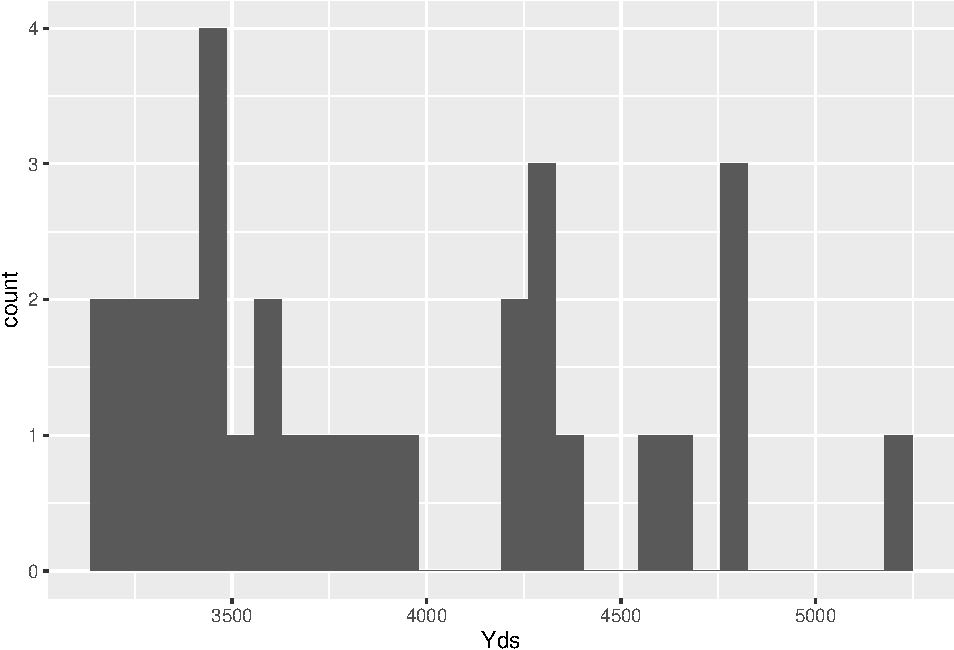
\includegraphics{textbook_files/figure-latex/hist-1.pdf}

Notice how \textbf{\%\textgreater\%} is used to \textbf{pipe} the dataset into ggplot. This is using the pipe function from the \textbf{dplyr} package.

\vfill
\newpage

By default, \textbf{geom\_histogram} uses 30 bins but this is customizable. Let's make the bins have a width of 200.

All good visualizations have good labels. Let's improve the axis labels and give the figure a title.

\begin{Shaded}
\begin{Highlighting}[]
\NormalTok{NFL\_2021\_Team\_Passing }\SpecialCharTok{\%\textgreater{}\%} \FunctionTok{ggplot}\NormalTok{(}\FunctionTok{aes}\NormalTok{(}\AttributeTok{x=}\NormalTok{Yds)) }\SpecialCharTok{+} 
  \FunctionTok{geom\_histogram}\NormalTok{(}\AttributeTok{binwidth =} \DecValTok{200}\NormalTok{) }\SpecialCharTok{+}
  \FunctionTok{labs}\NormalTok{(}\AttributeTok{x=}\StringTok{"Team Passing Yards"}\NormalTok{,}\AttributeTok{y=}\StringTok{"Team Passing Touchdowns"}\NormalTok{,}\AttributeTok{title=}\StringTok{"NFL Team Passing Yards, 2021"}\NormalTok{)}
\end{Highlighting}
\end{Shaded}

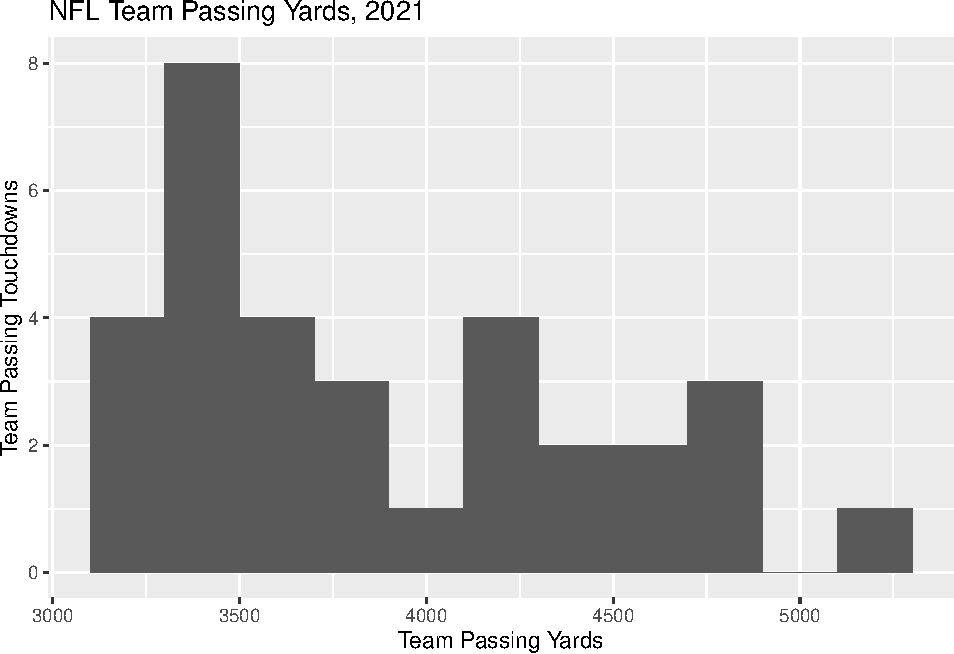
\includegraphics{textbook_files/figure-latex/hist2-1.pdf}

\vfill
\newpage

We also have numerous options to change the appearance of plots when using \textbf{ggplot}. Let's change the bins color to \emph{blue} and change the bin borders to \emph{white}.

\begin{Shaded}
\begin{Highlighting}[]
\NormalTok{NFL\_2021\_Team\_Passing }\SpecialCharTok{\%\textgreater{}\%} \FunctionTok{ggplot}\NormalTok{(}\FunctionTok{aes}\NormalTok{(}\AttributeTok{x=}\NormalTok{Yds)) }\SpecialCharTok{+} 
  \FunctionTok{geom\_histogram}\NormalTok{(}\AttributeTok{color =} \StringTok{"white"}\NormalTok{, }\AttributeTok{fill =} \StringTok{"blue"}\NormalTok{, }\AttributeTok{binwidth =} \DecValTok{200}\NormalTok{) }\SpecialCharTok{+}
  \FunctionTok{labs}\NormalTok{(}\AttributeTok{x=}\StringTok{"Team Passing Yards"}\NormalTok{, }\AttributeTok{y=}\StringTok{"Team Passing Touchdowns"}\NormalTok{, }\AttributeTok{title=}\StringTok{"NFL Team Passing Yards, 2021"}\NormalTok{)}
\end{Highlighting}
\end{Shaded}

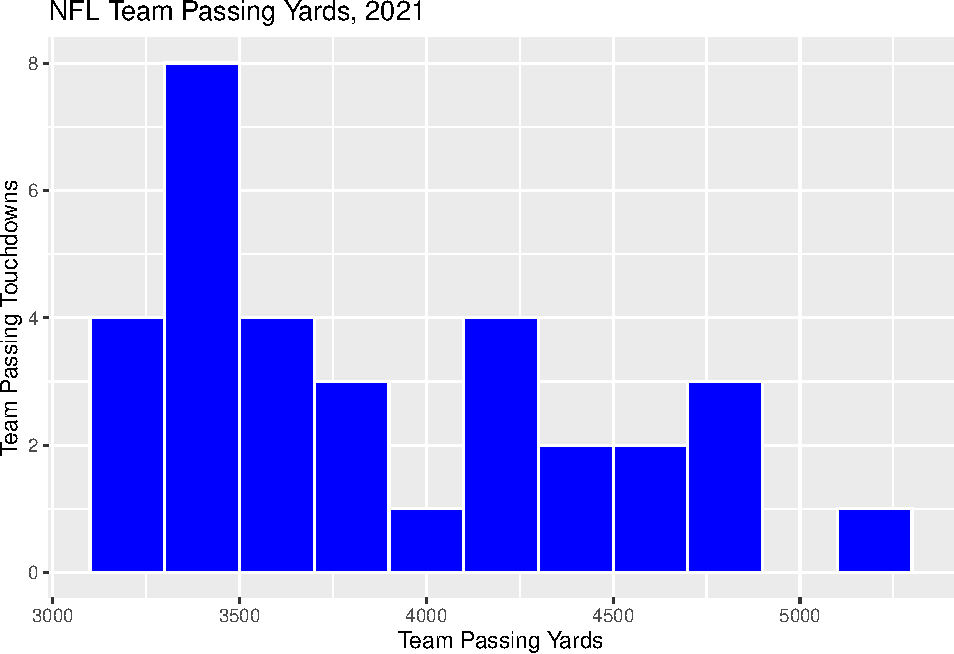
\includegraphics{textbook_files/figure-latex/hist3-1.pdf}
\end{example}

\vfill
\newpage

\hypertarget{bar-plots}{%
\subsection{Bar Plots}\label{bar-plots}}

We can also create bar plots using ggplot using the \textbf{geom\_bar} function.

\begin{example}
Create a bar plot with teams on the horizontal axis and passing touchdowns on the vertical axis.

\begin{Shaded}
\begin{Highlighting}[]
\NormalTok{NFL\_2021\_Team\_Passing }\SpecialCharTok{\%\textgreater{}\%} \FunctionTok{ggplot}\NormalTok{(}\FunctionTok{aes}\NormalTok{(}\AttributeTok{x=}\NormalTok{Tm,}\AttributeTok{y=}\NormalTok{Yds)) }\SpecialCharTok{+}
  \FunctionTok{geom\_bar}\NormalTok{(}\AttributeTok{stat=}\StringTok{"identity"}\NormalTok{)}
\end{Highlighting}
\end{Shaded}

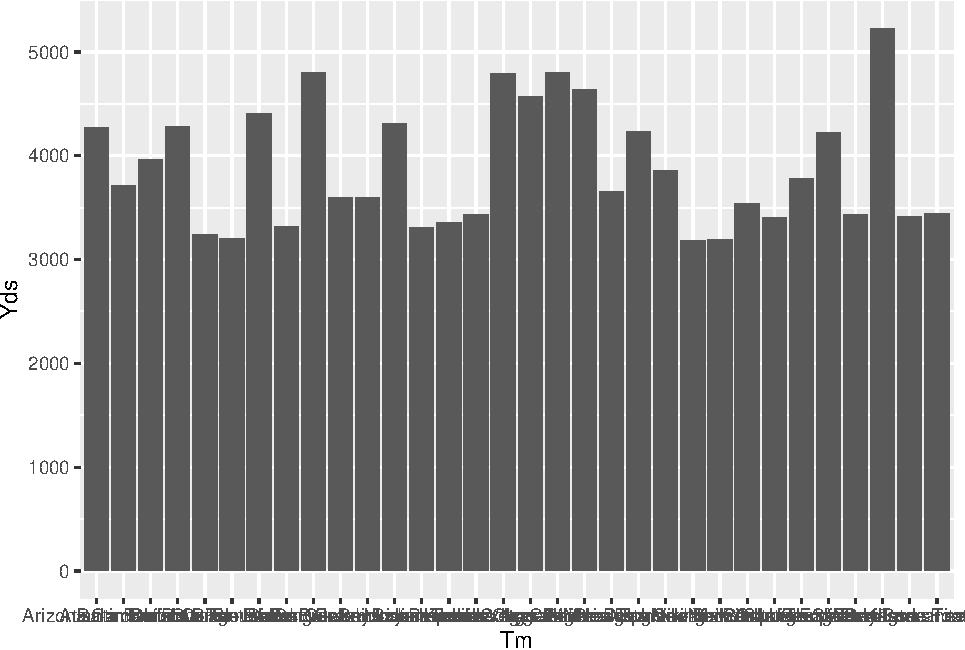
\includegraphics{textbook_files/figure-latex/bar-1.pdf}

\vfill
\newpage

The team labels are a complete mess. Let's fix this and make some adjustments to the axis labels and figure title.

\begin{Shaded}
\begin{Highlighting}[]
\NormalTok{NFL\_2021\_Team\_Passing }\SpecialCharTok{\%\textgreater{}\%} \FunctionTok{ggplot}\NormalTok{(}\FunctionTok{aes}\NormalTok{(}\AttributeTok{x=}\NormalTok{Tm,}\AttributeTok{y=}\NormalTok{Yds)) }\SpecialCharTok{+}
  \FunctionTok{geom\_bar}\NormalTok{(}\AttributeTok{stat=}\StringTok{"identity"}\NormalTok{) }\SpecialCharTok{+} 
  \FunctionTok{labs}\NormalTok{(}\AttributeTok{x=}\StringTok{"Team"}\NormalTok{, }\AttributeTok{y=}\StringTok{"Team Passing Yards"}\NormalTok{, }
       \AttributeTok{title=}\StringTok{"NFL Team Passing Yards, 2021"}\NormalTok{) }\SpecialCharTok{+}
  \FunctionTok{theme}\NormalTok{(}\AttributeTok{axis.text.x =} \FunctionTok{element\_text}\NormalTok{(}\AttributeTok{angle =} \DecValTok{90}\NormalTok{, }\AttributeTok{vjust =} \FloatTok{0.5}\NormalTok{, }\AttributeTok{hjust=}\DecValTok{1}\NormalTok{))}
\end{Highlighting}
\end{Shaded}

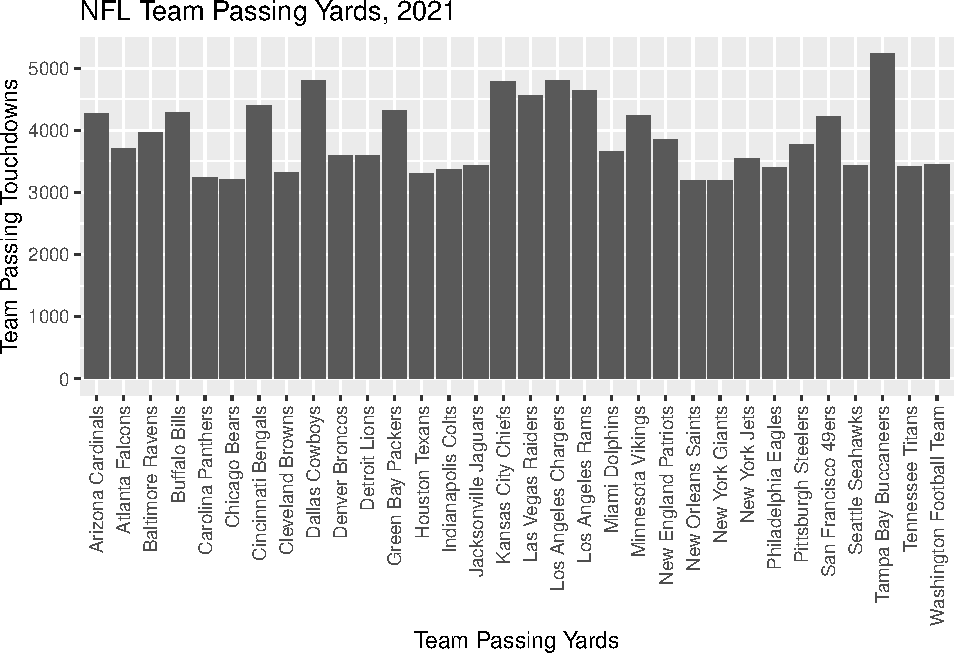
\includegraphics{textbook_files/figure-latex/bar2-1.pdf}

\vfill
\newpage

We can flip this graph if we like as well. Note that when we flip the graph, our labels get in reverse ordering, so this can be fixed using \textbf{fct\_rev()} which is part of the \textbf{forcats} package.

\begin{Shaded}
\begin{Highlighting}[]
\NormalTok{NFL\_2021\_Team\_Passing }\SpecialCharTok{\%\textgreater{}\%} 
  \FunctionTok{ggplot}\NormalTok{(}\FunctionTok{aes}\NormalTok{(}\AttributeTok{x=}\FunctionTok{fct\_rev}\NormalTok{(Tm),}\AttributeTok{y=}\NormalTok{Yds)) }\SpecialCharTok{+}
  \FunctionTok{geom\_bar}\NormalTok{(}\AttributeTok{stat=}\StringTok{"identity"}\NormalTok{) }\SpecialCharTok{+}
  \FunctionTok{labs}\NormalTok{(}\AttributeTok{x=}\StringTok{"Team Passing Yards"}\NormalTok{,}\AttributeTok{y=}\StringTok{"Team"}\NormalTok{,}\AttributeTok{title=}\StringTok{"NFL Team Passing Yards, 2021"}\NormalTok{) }\SpecialCharTok{+}
  \FunctionTok{coord\_flip}\NormalTok{()}
\end{Highlighting}
\end{Shaded}

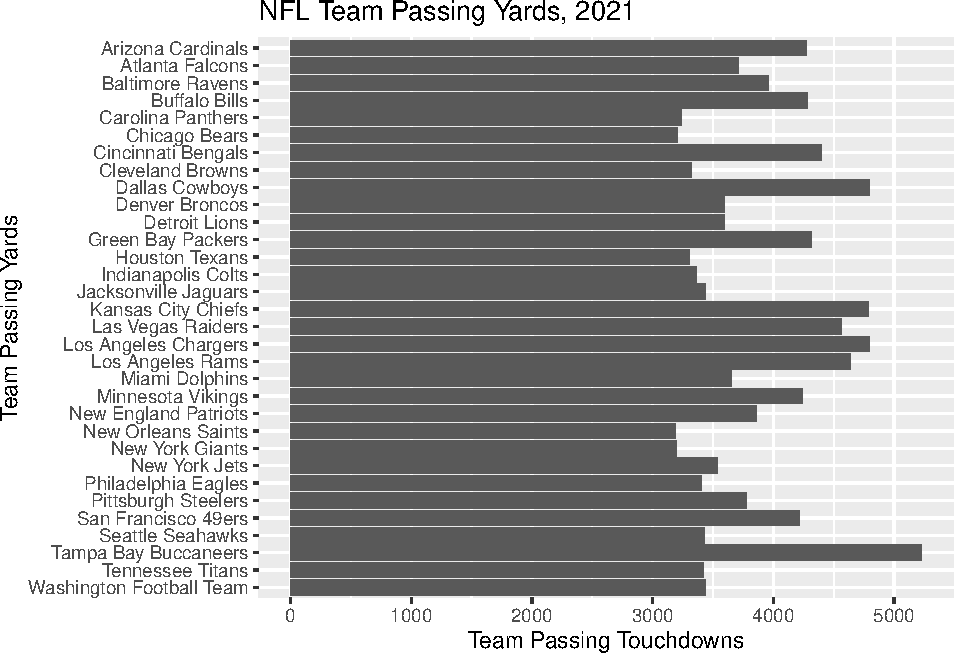
\includegraphics{textbook_files/figure-latex/bar3-1.pdf}
\end{example}

\vfill
\newpage

We can also order the teams from most team passing touchdowns to least using the \texttt{forcats} package.

\begin{Shaded}
\begin{Highlighting}[]
\NormalTok{NFL\_2021\_Team\_Passing }\SpecialCharTok{\%\textgreater{}\%} \FunctionTok{mutate}\NormalTok{(}\AttributeTok{Tm =} \FunctionTok{fct\_reorder}\NormalTok{(Tm,Yds)) }\SpecialCharTok{\%\textgreater{}\%}
  \FunctionTok{ggplot}\NormalTok{(}\FunctionTok{aes}\NormalTok{(}\AttributeTok{x=}\NormalTok{Tm,}\AttributeTok{y=}\NormalTok{Yds)) }\SpecialCharTok{+}
  \FunctionTok{geom\_bar}\NormalTok{(}\AttributeTok{stat=}\StringTok{"identity"}\NormalTok{) }\SpecialCharTok{+}
  \FunctionTok{labs}\NormalTok{(}\AttributeTok{x=}\StringTok{"Team Passing Yards"}\NormalTok{,}\AttributeTok{y=}\StringTok{"Team Passing Yards"}\NormalTok{,}\AttributeTok{title=}\StringTok{"NFL Team Passing Yards, 2021"}\NormalTok{) }\SpecialCharTok{+}
  \FunctionTok{coord\_flip}\NormalTok{()}
\end{Highlighting}
\end{Shaded}

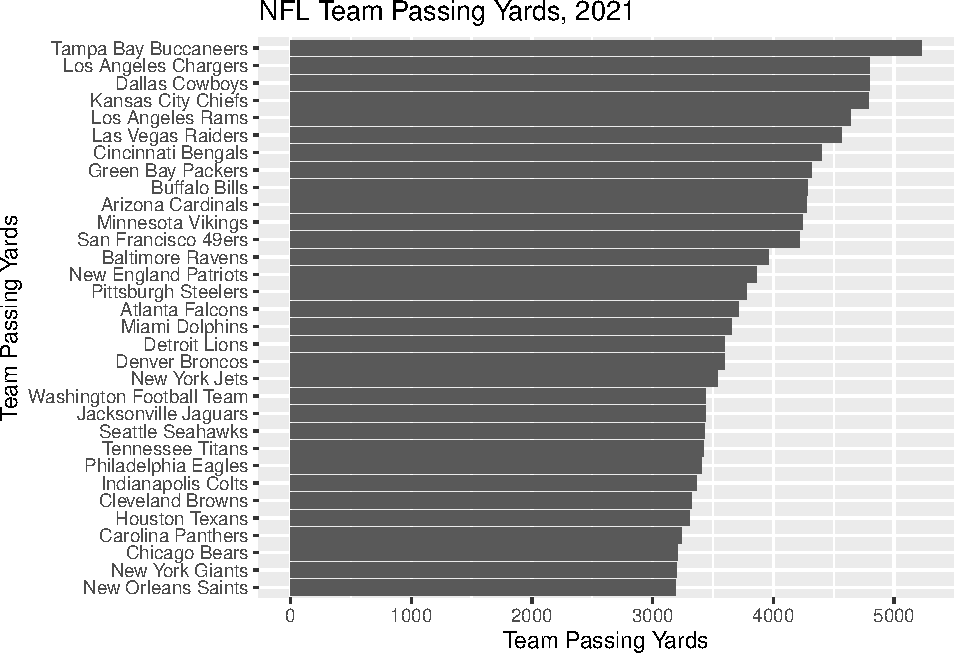
\includegraphics{textbook_files/figure-latex/unnamed-chunk-10-1.pdf}

\vfill
\newpage

\hypertarget{scatter-plots}{%
\subsection{Scatter Plots}\label{scatter-plots}}

Another common and useful visualization is a scatterplot which shows the relationship between two numeric variable. In ggplot, you use \textbf{geom\_point()}.

\begin{example}
Create a scatterplot of Team Passing Yards and Team Passing Touchdowns from the NFL 2021 dataset.

\begin{Shaded}
\begin{Highlighting}[]
\NormalTok{NFL\_2021\_Team\_Passing }\SpecialCharTok{\%\textgreater{}\%}
  \FunctionTok{ggplot}\NormalTok{(}\FunctionTok{aes}\NormalTok{(}\AttributeTok{x=}\NormalTok{Yds,}\AttributeTok{y=}\NormalTok{TD,}\AttributeTok{label=}\NormalTok{Tm)) }\SpecialCharTok{+} 
  \FunctionTok{geom\_point}\NormalTok{() }\SpecialCharTok{+}
  \FunctionTok{labs}\NormalTok{(}\AttributeTok{x=}\StringTok{"Team Passing Yards"}\NormalTok{,}\AttributeTok{y=}\StringTok{"Team Passing Touchdowns"}\NormalTok{,}\AttributeTok{title=}\StringTok{"NFL Team Passing Yards, 2021"}\NormalTok{)}
\end{Highlighting}
\end{Shaded}

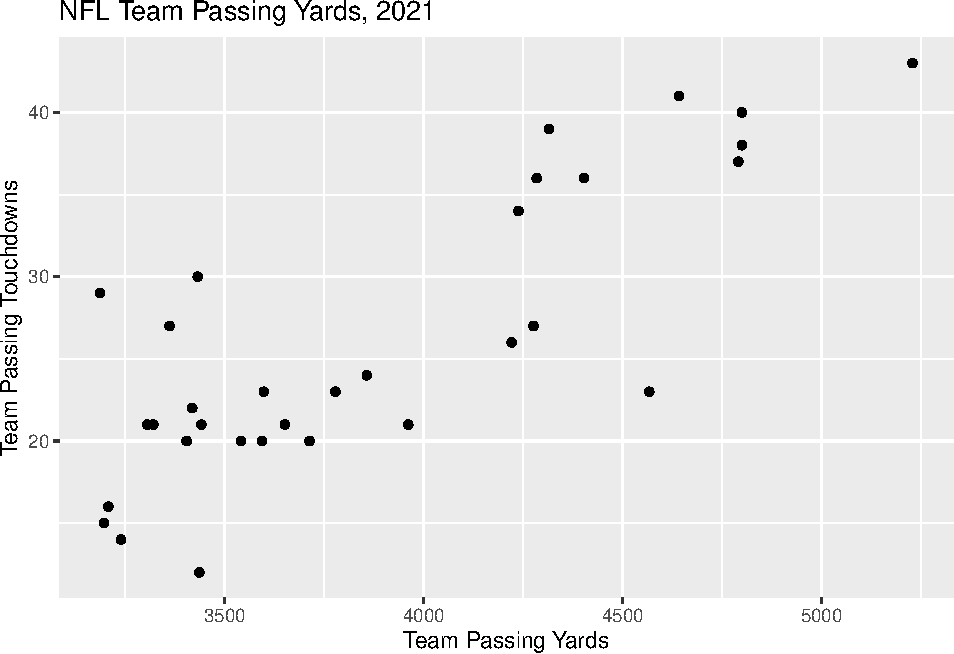
\includegraphics{textbook_files/figure-latex/scatter1-1.pdf}

\vfill
\newpage

We may want to include team labels on this plot, however, it can get messy very quickly with a lot of points.

\begin{Shaded}
\begin{Highlighting}[]
\NormalTok{NFL\_2021\_Team\_Passing }\SpecialCharTok{\%\textgreater{}\%}
  \FunctionTok{ggplot}\NormalTok{(}\FunctionTok{aes}\NormalTok{(}\AttributeTok{x=}\NormalTok{Yds,}\AttributeTok{y=}\NormalTok{TD,}\AttributeTok{label=}\NormalTok{Tm)) }\SpecialCharTok{+} 
  \FunctionTok{geom\_point}\NormalTok{() }\SpecialCharTok{+}
  \FunctionTok{labs}\NormalTok{(}\AttributeTok{x=}\StringTok{"Team Passing Yards"}\NormalTok{,}\AttributeTok{y=}\StringTok{"Team Passing Touchdowns"}\NormalTok{,}\AttributeTok{title=}\StringTok{"NFL Team Passing Yards, 2021"}\NormalTok{) }\SpecialCharTok{+}
  \FunctionTok{geom\_text}\NormalTok{()}
\end{Highlighting}
\end{Shaded}

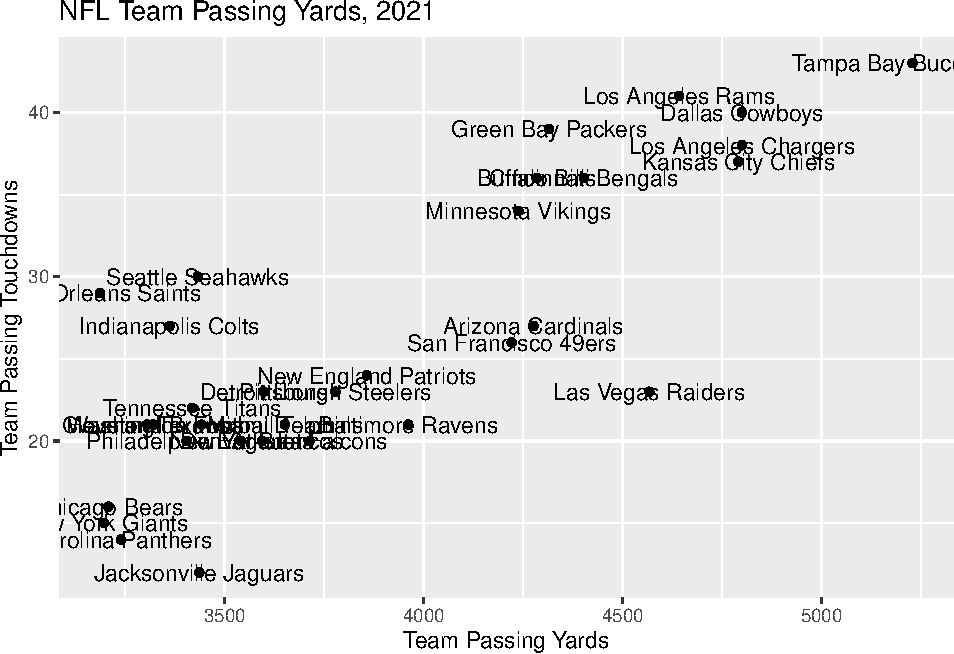
\includegraphics{textbook_files/figure-latex/scatter2-1.pdf}

\vfill
\newpage

Many sports leagues have around 30 teams, so a clean scatterplot with labels can be tricky to make. Here are some options below.

\begin{Shaded}
\begin{Highlighting}[]
\CommentTok{\# install ggrepel package}
\FunctionTok{library}\NormalTok{(ggrepel)}
\NormalTok{NFL\_2021\_Team\_Passing }\SpecialCharTok{\%\textgreater{}\%}
  \FunctionTok{ggplot}\NormalTok{(}\FunctionTok{aes}\NormalTok{(}\AttributeTok{x=}\NormalTok{Yds,}\AttributeTok{y=}\NormalTok{TD,}\AttributeTok{label=}\NormalTok{Tm)) }\SpecialCharTok{+} 
  \FunctionTok{geom\_point}\NormalTok{() }\SpecialCharTok{+}
  \FunctionTok{labs}\NormalTok{(}\AttributeTok{x=}\StringTok{"Team Passing Yards"}\NormalTok{,}\AttributeTok{y=}\StringTok{"Team Passing Touchdowns"}\NormalTok{,}\AttributeTok{title=}\StringTok{"NFL Team Passing Yards, 2021"}\NormalTok{) }\SpecialCharTok{+}
  \FunctionTok{geom\_text\_repel}\NormalTok{()}
\end{Highlighting}
\end{Shaded}

\begin{verbatim}
## Warning: ggrepel: 9 unlabeled data points (too many overlaps). Consider
## increasing max.overlaps
\end{verbatim}

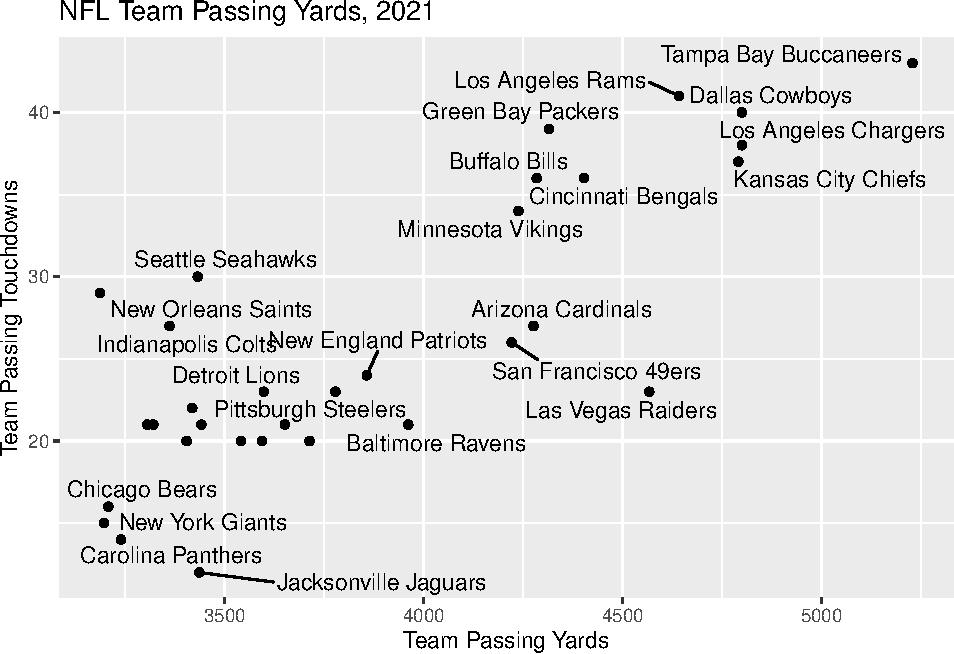
\includegraphics{textbook_files/figure-latex/scatter3-1.pdf}

\begin{Shaded}
\begin{Highlighting}[]
\NormalTok{NFL\_2021\_Team\_Passing}\SpecialCharTok{$}\NormalTok{Abbr }\OtherTok{\textless{}{-}} \FunctionTok{c}\NormalTok{(}\StringTok{"TB"}\NormalTok{,}\StringTok{"LAC"}\NormalTok{,}\StringTok{"DAL"}\NormalTok{,}\StringTok{"KC"}\NormalTok{,}\StringTok{"LAR"}\NormalTok{,}\StringTok{"LV"}\NormalTok{,}\StringTok{"CIN"}\NormalTok{,}\StringTok{"GB"}\NormalTok{,}\StringTok{"BUF"}\NormalTok{,}\StringTok{"AZ"}\NormalTok{,}\StringTok{"MN"}\NormalTok{,}\StringTok{"SF"}\NormalTok{,}
                                \StringTok{"BAL"}\NormalTok{,}\StringTok{"NE"}\NormalTok{,}\StringTok{"PIT"}\NormalTok{,}\StringTok{"ATL"}\NormalTok{,}\StringTok{"MIA"}\NormalTok{,}\StringTok{"DET"}\NormalTok{,}\StringTok{"DEN"}\NormalTok{,}\StringTok{"NYJ"}\NormalTok{,}\StringTok{"WAS"}\NormalTok{,}\StringTok{"JAC"}\NormalTok{,}\StringTok{"SEA"}\NormalTok{,}
                                \StringTok{"TEN"}\NormalTok{,}\StringTok{"PHI"}\NormalTok{,}\StringTok{"IND"}\NormalTok{,}\StringTok{"CLE"}\NormalTok{,}\StringTok{"HOU"}\NormalTok{,}\StringTok{"CAR"}\NormalTok{,}\StringTok{"CHI"}\NormalTok{,}\StringTok{"NYG"}\NormalTok{,}\StringTok{"NO"}\NormalTok{)}
\NormalTok{NFL\_2021\_Team\_Passing }\SpecialCharTok{\%\textgreater{}\%}
  \FunctionTok{ggplot}\NormalTok{(}\FunctionTok{aes}\NormalTok{(}\AttributeTok{x=}\NormalTok{Yds,}\AttributeTok{y=}\NormalTok{TD,}\AttributeTok{label=}\NormalTok{Abbr)) }\SpecialCharTok{+} 
  \FunctionTok{geom\_point}\NormalTok{() }\SpecialCharTok{+}
  \FunctionTok{scale\_x\_continuous}\NormalTok{(}\AttributeTok{limits=}\FunctionTok{c}\NormalTok{(}\DecValTok{2750}\NormalTok{,}\DecValTok{5250}\NormalTok{)) }\SpecialCharTok{+}
  \FunctionTok{labs}\NormalTok{(}\AttributeTok{x=}\StringTok{"Team Passing Yards"}\NormalTok{,}\AttributeTok{y=}\StringTok{"Team Passing Touchdowns"}\NormalTok{,}\AttributeTok{title=}\StringTok{"NFL Team Passing Yards, 2021"}\NormalTok{) }\SpecialCharTok{+}
  \FunctionTok{geom\_text\_repel}\NormalTok{(}\AttributeTok{box.padding =} \FloatTok{0.3}\NormalTok{) }
\end{Highlighting}
\end{Shaded}

\begin{verbatim}
## Warning: ggrepel: 1 unlabeled data points (too many overlaps). Consider
## increasing max.overlaps
\end{verbatim}

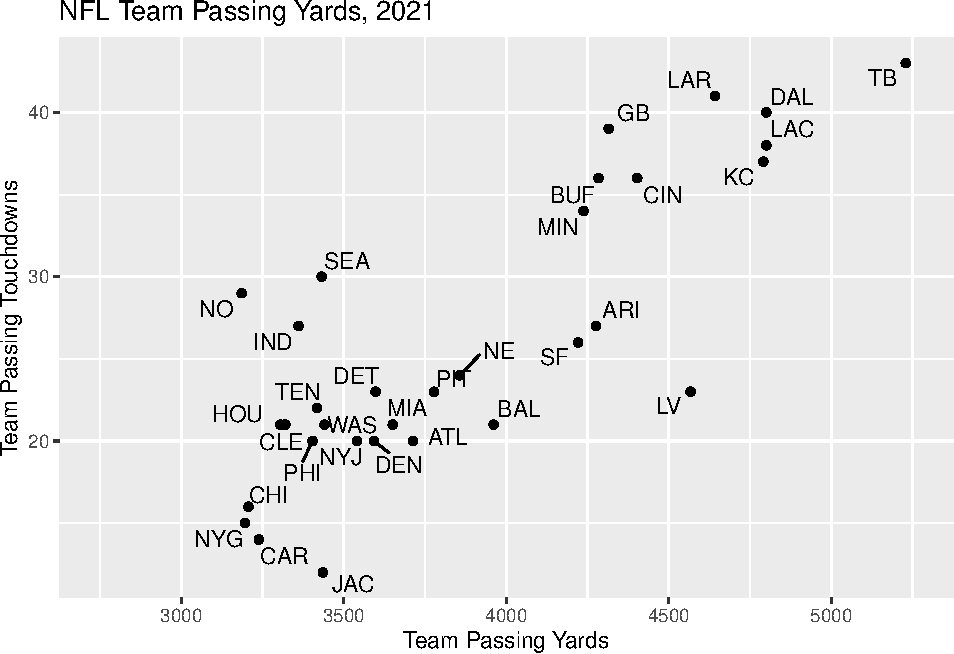
\includegraphics{textbook_files/figure-latex/scatter4-1.pdf}
\end{example}

\newpage

\hypertarget{kable-tables}{%
\subsection{Kable Tables}\label{kable-tables}}

We can build nice tables using \texttt{kableR} and \texttt{kableExtra}. Let's look at a few options.

\begin{Shaded}
\begin{Highlighting}[]
\CommentTok{\# Use a smaller dataset as an example}
\NormalTok{NFL21 }\OtherTok{\textless{}{-}}\NormalTok{ NFL\_2021\_Team\_Passing }\SpecialCharTok{\%\textgreater{}\%} \FunctionTok{select}\NormalTok{(}\DecValTok{2}\SpecialCharTok{:}\DecValTok{8}\NormalTok{) }\SpecialCharTok{\%\textgreater{}\%} \FunctionTok{slice\_head}\NormalTok{(}\AttributeTok{n =} \DecValTok{5}\NormalTok{)}

\CommentTok{\# Default output for tabular data}
\NormalTok{NFL21}
\end{Highlighting}
\end{Shaded}

\begin{verbatim}
## # A tibble: 5 x 7
##   Tm                       G   Cmp   Att `Cmp%`   Yds    TD
##   <chr>                <dbl> <dbl> <dbl>  <dbl> <dbl> <dbl>
## 1 Tampa Bay Buccaneers    17   492   731   67.3  5229    43
## 2 Los Angeles Chargers    17   443   674   65.7  4800    38
## 3 Dallas Cowboys          17   444   647   68.6  4800    40
## 4 Kansas City Chiefs      17   448   675   66.4  4791    37
## 5 Los Angeles Rams        17   406   607   66.9  4642    41
\end{verbatim}

You can find additional details on customizing kable tables at ~\url{https://cran.r-project.org/web/packages/kableExtra/vignettes/awesome_table_in_pdf.pdf}

\begin{Shaded}
\begin{Highlighting}[]
\CommentTok{\# Output using Kable (with no additional options)}
\FunctionTok{library}\NormalTok{(kableExtra)}

\CommentTok{\# Output using Kable and Kable{-}Styling and some additional options}
\NormalTok{NFL21 }\SpecialCharTok{\%\textgreater{}\%} \FunctionTok{kable}\NormalTok{() }\SpecialCharTok{\%\textgreater{}\%} \FunctionTok{kable\_styling}\NormalTok{(}\AttributeTok{latex\_options=}\StringTok{"hold\_position"}\NormalTok{)}
\end{Highlighting}
\end{Shaded}

\begin{table}[!h]
\centering
\begin{tabular}{l|r|r|r|r|r|r}
\hline
Tm & G & Cmp & Att & Cmp\% & Yds & TD\\
\hline
Tampa Bay Buccaneers & 17 & 492 & 731 & 67.3 & 5229 & 43\\
\hline
Los Angeles Chargers & 17 & 443 & 674 & 65.7 & 4800 & 38\\
\hline
Dallas Cowboys & 17 & 444 & 647 & 68.6 & 4800 & 40\\
\hline
Kansas City Chiefs & 17 & 448 & 675 & 66.4 & 4791 & 37\\
\hline
Los Angeles Rams & 17 & 406 & 607 & 66.9 & 4642 & 41\\
\hline
\end{tabular}
\end{table}

\vfill
\newpage

If you are going to use kable tables frequently in a document, you can write a short function to set your default options. After I ran the function below, the function \texttt{kt} will produce a kable table with my options set.

\begin{Shaded}
\begin{Highlighting}[]
\CommentTok{\# kable table global setup}
\NormalTok{kt }\OtherTok{\textless{}{-}} \ControlFlowTok{function}\NormalTok{(data) \{}
\NormalTok{   knitr}\SpecialCharTok{::}\FunctionTok{kable}\NormalTok{(data, }\AttributeTok{digits=}\DecValTok{3}\NormalTok{, }\AttributeTok{align=}\FunctionTok{c}\NormalTok{(}\StringTok{\textquotesingle{}l\textquotesingle{}}\NormalTok{,}\StringTok{\textquotesingle{}c\textquotesingle{}}\NormalTok{,}\StringTok{\textquotesingle{}c\textquotesingle{}}\NormalTok{,}\StringTok{\textquotesingle{}c\textquotesingle{}}\NormalTok{,}\StringTok{\textquotesingle{}c\textquotesingle{}}\NormalTok{,}\StringTok{\textquotesingle{}c\textquotesingle{}}\NormalTok{,}\StringTok{\textquotesingle{}c\textquotesingle{}}\NormalTok{,}\StringTok{\textquotesingle{}c\textquotesingle{}}\NormalTok{,}\StringTok{\textquotesingle{}c\textquotesingle{}}\NormalTok{)) }\SpecialCharTok{\%\textgreater{}\%} \FunctionTok{kable\_styling}\NormalTok{(}\AttributeTok{bootstrap\_options=}\StringTok{\textquotesingle{}striped\textquotesingle{}}\NormalTok{, }\AttributeTok{latex\_options=}\StringTok{\textquotesingle{}HOLD\_position\textquotesingle{}}\NormalTok{, }\AttributeTok{full\_width =}\NormalTok{ F, }\AttributeTok{position =} \StringTok{"center"}\NormalTok{)}
\NormalTok{\}}
\end{Highlighting}
\end{Shaded}

\begin{Shaded}
\begin{Highlighting}[]
\NormalTok{NFL21 }\SpecialCharTok{\%\textgreater{}\%} \FunctionTok{kt}\NormalTok{()}
\end{Highlighting}
\end{Shaded}

\begin{table}[H]
\centering
\begin{tabular}{l|c|c|c|c|c|c}
\hline
Tm & G & Cmp & Att & Cmp\% & Yds & TD\\
\hline
Tampa Bay Buccaneers & 17 & 492 & 731 & 67.3 & 5229 & 43\\
\hline
Los Angeles Chargers & 17 & 443 & 674 & 65.7 & 4800 & 38\\
\hline
Dallas Cowboys & 17 & 444 & 647 & 68.6 & 4800 & 40\\
\hline
Kansas City Chiefs & 17 & 448 & 675 & 66.4 & 4791 & 37\\
\hline
Los Angeles Rams & 17 & 406 & 607 & 66.9 & 4642 & 41\\
\hline
\end{tabular}
\end{table}

\newpage

\hypertarget{baseball}{%
\section{Baseball}\label{baseball}}

Baseball rules YouTube video: \url{https://www.youtube.com/watch?v=skOsApsF0jQ\&t=63s}

\hypertarget{hitting-statistics}{%
\subsection{Hitting Statistics}\label{hitting-statistics}}

\hypertarget{basic-hitting-statistics}{%
\subsubsection{Basic Hitting Statistics}\label{basic-hitting-statistics}}

\begin{itemize}
\item
  \textbf{Plate Appearances} (PA): number of completed batting appearances
\item
  \textbf{At-Bats} (AB): Batting appearances, not including bases on balls, hit by pitch, sacrifices, interference, or obstruction
\item
  \textbf{Hits} (H): Times reached base because of a batted, fair ball without error by the defense
\item
  \textbf{Singles} (1B): Hits on which the batter reached first base safely without the contribution of a fielding error
\item
  \textbf{Doubles} (2B): Hits on which the batter reached second base safely without the contribution of a fielding error
\item
  \textbf{Triples} (3B): Hits on which the batter reached third base safely without the contribution of a fielding error
\item
  \textbf{Home Runs} (HR): Hits on which the batter successfully touched all four bases, without the contribution of a fielding error
\item
  \textbf{Total Bases} (TB): One for each single, two for each double, three for each triple, and four for each home run
\item
  \textbf{Hit by Pitch} (HBP): Times touched by a pitch and awarded first base as a result
\item
  \textbf{Sacrifice Fly} (SF): Number of fly ball outs which allow another runner to advance on the basepaths or score
\item
  \textbf{Base on Balls} (BB or Walk): Times receiving four balls and advancing to first base
\item
  \textbf{Intentional Base on Balls} (IBB or Intentional Walk): Times receiving four balls \emph{intentionally} and advancing to first base
\item
  \textbf{Strikeout} (K): Number of times that strike three is taken or swung at and missed, or bunted foul
\item
  \textbf{Runs} (R): Times reached home base legally and safely
\item
  \textbf{Runs Batted In} (RBI): Number of runners who scored due to a batters's action, except when batter grounded into double play or reached on an error
\item
  \textbf{Batting Average} (AVG or BA): Hits divided by at bats
\item
  \textbf{On Base Percentage/Average} (OBP or OBA): Times reached base (H + BB + HBP) divided by at bats plus walks plus hit by pitch plus sacrifice flies (AB + BB + HBP + SF)
\item
  \textbf{Slugging Percentage/Average} (SLG): Total bases divided by at-bats
\item
  \textbf{On-base Plus Slugging} (OPS): On-base percentage plus slugging average
\end{itemize}

\newpage

\hypertarget{advanced-baseball-hitting-statistics}{%
\subsubsection{Advanced Baseball Hitting Statistics}\label{advanced-baseball-hitting-statistics}}

\begin{itemize}
\item
  \textbf{Isolated Power} (ISO): Slugging percentage minus Batting average
\item
  \textbf{On-base Plus Slugging Plus} (OPS+): OPS normalized for park effects with 100 being league average
\item
  \textbf{Weighted On-Base Average} (wOBA): Hitting rate statistic that attempts to credit the hitter for the value of each outcome. The following formula can be updated each year based on the scoring environment. The following formula was updated for the 2021 season.
\end{itemize}

\[wOBA = \frac{0.69 \cdot (BB - IBB) + 0.719 \cdot HBP + 0.87 \cdot 1B + 1.217 \cdot 2B + 1.529 \cdot 3B + 1.94 \cdot HR}{AB + BB - IBB + SF + HBP}\]

\begin{itemize}
\tightlist
\item
  \textbf{Expected Weighted On-Base Average} (xwOBA): Hitting rate statistic that attempts to credit the hitter for the value of each \emph{expected} outcome based on Statcast data.
\end{itemize}

\hypertarget{pitching-statistics}{%
\subsection{Pitching Statistics}\label{pitching-statistics}}

\hypertarget{basic-pitching-statistics}{%
\subsubsection{Basic Pitching Statistics}\label{basic-pitching-statistics}}

\begin{itemize}
\item
  \textbf{Innings Pitched} (IP): Number of outs recorded while pitching divided by three
\item
  \textbf{Strikeout} (K): Number of batters who received strike three
\item
  \textbf{Base on Balls} (BB or Walk): Times pitching four balls, allowing the batter-runner to advance to first base
\item
  \textbf{Hits Allowed} (H): Total hits allowed
\item
  \textbf{Wins} (W): Number of games where pitcher was pitching while his team took the lead and went on to win
\item
  \textbf{Losses} (L): Number of games where pitcher was pitching while the opposing team took the lead, never lost the lead, and went on to win
\item
  \textbf{Earned Runs} (ER): Number of runs that did not occur as a result of errors or passed balls
\item
  \textbf{Earned Run Average} (ERA): Earned runs times innings in a game (usually nine) divided by innings pitched
\item
  \textbf{Walks and Hits Per Inning Pitched} (WHIP): Walks plus hits allowed divided by innings pitched
\end{itemize}

\hypertarget{advanced-pitching-statistics}{%
\subsubsection{Advanced Pitching Statistics}\label{advanced-pitching-statistics}}

\begin{itemize}
\tightlist
\item
  \textbf{Fielding Independent Pitching} (FIP): Statistic that estimates a pitcher's run prevention independent of the performance of the defense
\end{itemize}

\[FIP = \frac{13 \cdot HR + 3 \cdot (BB + HBP) - 2 \cdot K}{IP} + FIP_{constant}\]

The \(FIP_{constant}\) is generally around 3.10 and is put FIP on a scale similar to ERA.

\begin{itemize}
\tightlist
\item
  \textbf{Expected Fielding Independent Pitching} (xFIP): Statistic that estimates a pitcher's expected run prevention independent of the performance of the defense
\end{itemize}

\[xFIP = \frac{13 \cdot (Fly Balls \cdot LgHR/FB\%)+3 \cdot (BB + HBP) - 2 \cdot K}{IP} + FIP_{constant}\]

\hypertarget{wins-above-replacement}{%
\subsection{Wins Above Replacement}\label{wins-above-replacement}}

\begin{itemize}
\tightlist
\item
  \textbf{Wins Above Replacement} (WAR): Estimated number of wins that a player has outperformed a replacement player by with the same playing time. This is one of the most crucial statistics in Sabermetrics.
\end{itemize}

More about WAR from Fangraphs: \url{https://library.fangraphs.com/misc/war/}

\emph{References:}\\
\url{https://www.baseball-reference.com/bullpen/Baseball_statistics}\strut \\
\url{https://blogs.fangraphs.com/glossary/}\strut \\
\url{https://library.fangraphs.com/fangraphs-library-glossary/}\strut \\

\newpage

\hypertarget{calculating-hitting-statistics}{%
\subsection{Calculating Hitting Statistics}\label{calculating-hitting-statistics}}

\begin{example}
Using the Colorado Rockies 2021 individual hitting statistics, calculate the AVG, OBA, SLG, OPS, ISO, wOBA.
\end{example}

\begin{Shaded}
\begin{Highlighting}[]
\CommentTok{\# load data file and look at the header}
\NormalTok{rox21 }\OtherTok{\textless{}{-}} \FunctionTok{read\_csv}\NormalTok{(}\StringTok{"data/rockies\_hitting2021.csv"}\NormalTok{)}
\NormalTok{rox21 }\SpecialCharTok{\%\textgreater{}\%} \FunctionTok{slice\_head}\NormalTok{(}\AttributeTok{n=}\DecValTok{5}\NormalTok{) }\SpecialCharTok{\%\textgreater{}\%} \FunctionTok{kt}\NormalTok{()}
\end{Highlighting}
\end{Shaded}

\begin{table}[H]
\centering
\begin{tabular}{l|c|c|c|c|c|c|c|c|l|c|c|c|c|c}
\hline
Name & PA & AB & R & H & 2B & 3B & HR & RBI & BB & IBB & SO & HBP & SF & oWAR\\
\hline
Elias Diaz & 371 & 338 & 52 & 83 & 18 & 1 & 18 & 44 & 30 & 1 & 60 & 2 & 1 & 1.1\\
\hline
C.J. Cron & 547 & 470 & 70 & 132 & 31 & 1 & 28 & 92 & 60 & 3 & 117 & 13 & 4 & 3.1\\
\hline
Brendan Rodgers & 415 & 387 & 49 & 110 & 21 & 3 & 15 & 51 & 19 & 0 & 84 & 7 & 2 & 1.9\\
\hline
Trevor Story & 595 & 526 & 88 & 132 & 34 & 5 & 24 & 75 & 53 & 2 & 139 & 11 & 5 & 3.4\\
\hline
Ryan McMahon* & 596 & 528 & 80 & 134 & 32 & 1 & 23 & 86 & 59 & 2 & 147 & 4 & 5 & 1.7\\
\hline
\end{tabular}
\end{table}

\begin{Shaded}
\begin{Highlighting}[]
\CommentTok{\# Create new variables using the mutate function}
\NormalTok{rox21 }\OtherTok{\textless{}{-}}\NormalTok{ rox21 }\SpecialCharTok{\%\textgreater{}\%} 
  \FunctionTok{mutate}\NormalTok{(}\AttributeTok{AVG =}\NormalTok{ H}\SpecialCharTok{/}\NormalTok{AB,}\DecValTok{3}\NormalTok{) }\SpecialCharTok{\%\textgreater{}\%}
  \FunctionTok{mutate}\NormalTok{(}\AttributeTok{OBA =}\NormalTok{ (H }\SpecialCharTok{+}\NormalTok{ BB }\SpecialCharTok{+}\NormalTok{ HBP)}\SpecialCharTok{/}\NormalTok{(AB }\SpecialCharTok{+}\NormalTok{ BB }\SpecialCharTok{+}\NormalTok{ HBP }\SpecialCharTok{+}\NormalTok{ SF)) }\SpecialCharTok{\%\textgreater{}\%}
  \FunctionTok{mutate}\NormalTok{(}\AttributeTok{SLG =}\NormalTok{ ((H}\SpecialCharTok{{-}}\StringTok{\textasciigrave{}}\AttributeTok{2B}\StringTok{\textasciigrave{}}\SpecialCharTok{{-}}\StringTok{\textasciigrave{}}\AttributeTok{3B}\StringTok{\textasciigrave{}}\SpecialCharTok{{-}}\NormalTok{HR) }\SpecialCharTok{+} \DecValTok{2}\SpecialCharTok{*}\StringTok{\textasciigrave{}}\AttributeTok{2B}\StringTok{\textasciigrave{}} \SpecialCharTok{+} \DecValTok{3}\SpecialCharTok{*}\StringTok{\textasciigrave{}}\AttributeTok{3B}\StringTok{\textasciigrave{}} \SpecialCharTok{+} \DecValTok{4}\SpecialCharTok{*}\NormalTok{HR)}\SpecialCharTok{/}\NormalTok{AB) }\SpecialCharTok{\%\textgreater{}\%}
  \FunctionTok{mutate}\NormalTok{(}\AttributeTok{OPS =}\NormalTok{ SLG }\SpecialCharTok{+}\NormalTok{ OBA) }\SpecialCharTok{\%\textgreater{}\%}
  \FunctionTok{mutate}\NormalTok{(}\AttributeTok{wOBA =}\NormalTok{ (}\FloatTok{0.692} \SpecialCharTok{*}\NormalTok{ (BB }\SpecialCharTok{{-}}\NormalTok{ IBB) }\SpecialCharTok{+} \FloatTok{0.722} \SpecialCharTok{*}\NormalTok{ HBP }\SpecialCharTok{+} \FloatTok{0.879} \SpecialCharTok{*}\NormalTok{ (H}\SpecialCharTok{{-}}\StringTok{\textasciigrave{}}\AttributeTok{2B}\StringTok{\textasciigrave{}}\SpecialCharTok{{-}}\StringTok{\textasciigrave{}}\AttributeTok{3B}\StringTok{\textasciigrave{}}\SpecialCharTok{{-}}\NormalTok{HR) }\SpecialCharTok{+} \FloatTok{1.242} \SpecialCharTok{*} \StringTok{\textasciigrave{}}\AttributeTok{2B}\StringTok{\textasciigrave{}} \SpecialCharTok{+} \FloatTok{1.568} \SpecialCharTok{*} \StringTok{\textasciigrave{}}\AttributeTok{3B}\StringTok{\textasciigrave{}} \SpecialCharTok{+} \FloatTok{2.007} \SpecialCharTok{*}\NormalTok{ HR)}\SpecialCharTok{/}\NormalTok{(AB }\SpecialCharTok{+}\NormalTok{ BB }\SpecialCharTok{{-}}\NormalTok{ IBB }\SpecialCharTok{+}\NormalTok{ SF }\SpecialCharTok{+}\NormalTok{ HBP)) }\SpecialCharTok{\%\textgreater{}\%}
  \FunctionTok{mutate}\NormalTok{(}\AttributeTok{ISO =}\NormalTok{ SLG}\SpecialCharTok{{-}}\NormalTok{AVG)}
\NormalTok{rox21 }\SpecialCharTok{\%\textgreater{}\%} \FunctionTok{slice\_head}\NormalTok{(}\AttributeTok{n=}\DecValTok{5}\NormalTok{) }\SpecialCharTok{\%\textgreater{}\%} \FunctionTok{select}\NormalTok{(Name,PA,AVG,OBA,SLG,OPS,wOBA,ISO) }\SpecialCharTok{\%\textgreater{}\%} \FunctionTok{kt}\NormalTok{()}
\end{Highlighting}
\end{Shaded}

\begin{table}[H]
\centering
\begin{tabular}{l|c|c|c|c|c|c|c}
\hline
Name & PA & AVG & OBA & SLG & OPS & wOBA & ISO\\
\hline
Elias Diaz & 371 & 0.246 & 0.310 & 0.464 & 0.774 & 0.330 & 0.219\\
\hline
C.J. Cron & 547 & 0.281 & 0.375 & 0.530 & 0.905 & 0.383 & 0.249\\
\hline
Brendan Rodgers & 415 & 0.284 & 0.328 & 0.470 & 0.798 & 0.341 & 0.186\\
\hline
Trevor Story & 595 & 0.251 & 0.329 & 0.471 & 0.801 & 0.341 & 0.221\\
\hline
Ryan McMahon* & 596 & 0.254 & 0.331 & 0.449 & 0.779 & 0.334 & 0.195\\
\hline
\end{tabular}
\end{table}

\vfill
\newpage

\begin{example}
oWAR is Baseball Reference's offensive WAR statistic. Note that Baseball Reference and Fangraphs use different formulas when calculating WAR though their results are typically similar. For Rockies players with at least 100 at-bats in 2021, what hitting statistics are most and least correlated to oWAR?
\end{example}

\begin{Shaded}
\begin{Highlighting}[]
\CommentTok{\# Let\textquotesingle{}s remove players with less than 100 ABs}
\NormalTok{rox21\_100 }\OtherTok{\textless{}{-}}\NormalTok{ rox21 }\SpecialCharTok{\%\textgreater{}\%} \FunctionTok{filter}\NormalTok{(AB }\SpecialCharTok{\textgreater{}=} \DecValTok{100}\NormalTok{)}

\CommentTok{\# GGally package has a nice pairs plotting function}
\FunctionTok{library}\NormalTok{(}\StringTok{"GGally"}\NormalTok{)}

\CommentTok{\# Standard hitting statistics}
\NormalTok{rox21\_100 }\SpecialCharTok{\%\textgreater{}\%} \FunctionTok{select}\NormalTok{(oWAR,H,}\StringTok{\textasciigrave{}}\AttributeTok{2B}\StringTok{\textasciigrave{}}\NormalTok{,}\StringTok{\textasciigrave{}}\AttributeTok{3B}\StringTok{\textasciigrave{}}\NormalTok{,HR,R,RBI) }\SpecialCharTok{\%\textgreater{}\%} \FunctionTok{ggpairs}\NormalTok{() }\SpecialCharTok{+}
  \FunctionTok{theme}\NormalTok{(}\AttributeTok{axis.text.x =} \FunctionTok{element\_text}\NormalTok{(}\AttributeTok{angle =} \DecValTok{90}\NormalTok{, }\AttributeTok{hjust =} \DecValTok{1}\NormalTok{))}
\end{Highlighting}
\end{Shaded}

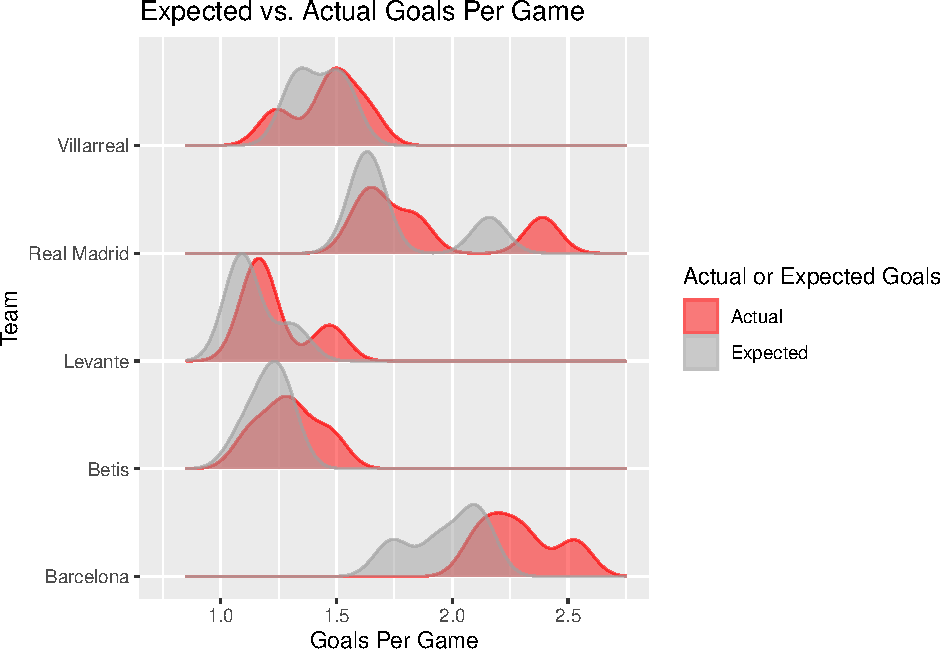
\includegraphics{textbook_files/figure-latex/unnamed-chunk-17-1.pdf}

\begin{Shaded}
\begin{Highlighting}[]
\CommentTok{\# Rate statistics}
\NormalTok{rox21\_100 }\SpecialCharTok{\%\textgreater{}\%} \FunctionTok{select}\NormalTok{(oWAR,AVG,OBA,SLG,OPS,wOBA) }\SpecialCharTok{\%\textgreater{}\%} \FunctionTok{ggpairs}\NormalTok{()}
\end{Highlighting}
\end{Shaded}

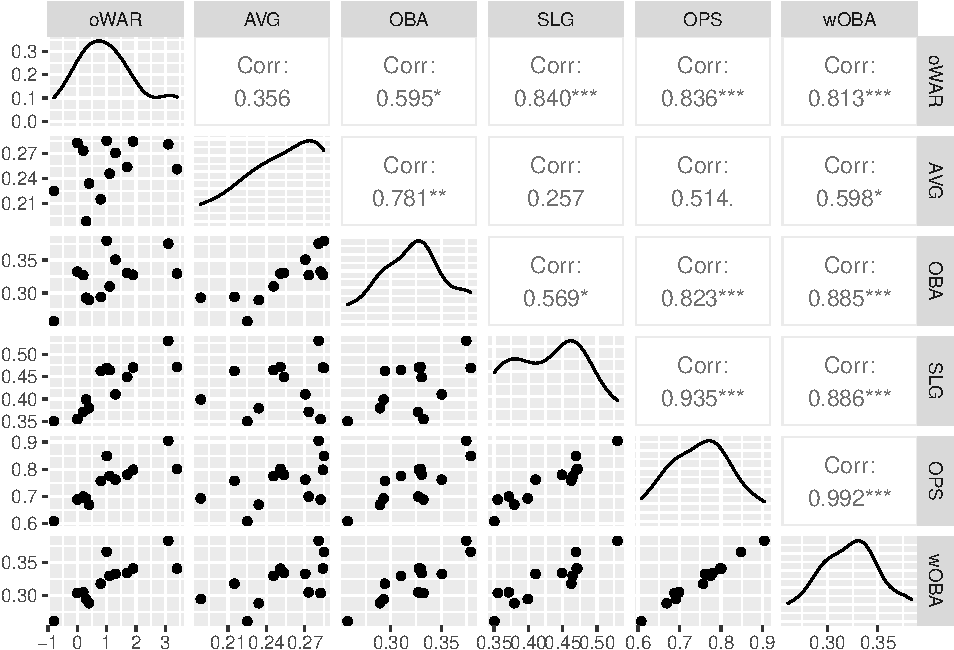
\includegraphics{textbook_files/figure-latex/unnamed-chunk-17-2.pdf}

\newpage

\hypertarget{evaluating-pitching-statistics}{%
\subsection{Evaluating Pitching Statistics}\label{evaluating-pitching-statistics}}

Earned run average (ERA) has been traditionally used to evaluate a pitcher, however, it has some flaws. First of all, it is highly dependent on the fielders playing behind the pitcher. If a pitcher's shortstop has poor range, he won't convert as many groundballs into outs as a shortstop with good range. ERA is also a noisy measurement in that can be affected easily by random luck.

To overcome some of the downsides of ERA, FIP and xFIP were developed to help reduce the variance (noise) of the measurement and to remove factors, like defense, that are not a function of the pitcher's ability.

Let's look at the twenty starting pitchers that had the most innings pitched in MLB for the total of the 2020 and 2021 seasons. We want to examine the year-to-year correlation between ERA, FIP, and xFIP.

\begin{Shaded}
\begin{Highlighting}[]
\NormalTok{pitchers2021 }\OtherTok{\textless{}{-}} \FunctionTok{read\_csv}\NormalTok{(}\StringTok{"data/MLBpitchers20{-}21.csv"}\NormalTok{)}
\NormalTok{pitchers2021 }\SpecialCharTok{\%\textgreater{}\%} \FunctionTok{slice\_head}\NormalTok{(}\AttributeTok{n=}\DecValTok{5}\NormalTok{) }\SpecialCharTok{\%\textgreater{}\%} \FunctionTok{kt}\NormalTok{()}
\end{Highlighting}
\end{Shaded}

\begin{table}[H]
\centering
\begin{tabular}{l|c|c|c|c|c|c}
\hline
Player & ERA20 & FIP20 & xFIP20 & ERA21 & FIP21 & xFIP21\\
\hline
Zack Wheeler & 2.92 & 3.22 & 3.76 & 2.78 & 2.59 & 2.84\\
\hline
Adam Wainwright & 3.15 & 4.11 & 4.23 & 3.05 & 3.66 & 3.87\\
\hline
Kyle Hendricks & 2.88 & 3.55 & 3.78 & 0.77 & 4.89 & 4.61\\
\hline
German Marquez & 3.75 & 3.28 & 3.83 & 4.40 & 3.86 & 3.64\\
\hline
Luis Castillo & 3.21 & 2.65 & 2.82 & 3.98 & 3.75 & 3.63\\
\hline
\end{tabular}
\end{table}

\vfill
\newpage

Let's look at the correlations between these variables, paying close attention to what variables are most correlated with ERA20, a pitcher's ERA in 2020.

\begin{Shaded}
\begin{Highlighting}[]
\NormalTok{pitchers2021 }\SpecialCharTok{\%\textgreater{}\%}
  \FunctionTok{select}\NormalTok{(}\SpecialCharTok{{-}}\NormalTok{Player) }\SpecialCharTok{\%\textgreater{}\%}
  \FunctionTok{ggpairs}\NormalTok{(}\AttributeTok{title=}\StringTok{"Correlation plot of pitching statistics, MLB 2020{-}2021"}\NormalTok{)}
\end{Highlighting}
\end{Shaded}

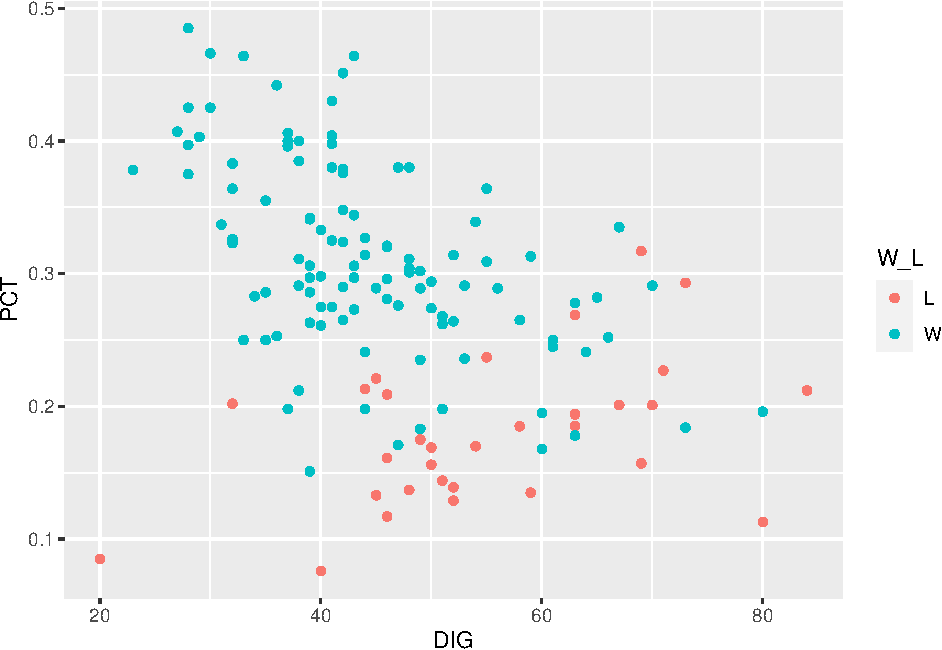
\includegraphics{textbook_files/figure-latex/unnamed-chunk-19-1.pdf}

This is a small dataset that only contains twenty pitchers (samples), but you will notice that ERA20 is more highly correlated with FIP21 and xFIP21 than ERA21. In other words, FIP and xFIP are likely better predictors of ERA success in the future rather than ERA success in the past.

\vfill
\newpage

\hypertarget{football}{%
\section{Football}\label{football}}

\href{https://www.youtube.com/watch?v=Ddwp1HyEFRE}{Link to YouTube video describing football rules}

\hypertarget{basic-football-statistics}{%
\subsection{Basic Football Statistics}\label{basic-football-statistics}}

\begin{itemize}
\item
  \textbf{Yards} (Yd): Number of yards gained from the line of scrimmage (can be broken down into Offense: Rushing and Passing Yards, Defense: Rushing and Passing Yards Allowed, and Special Teams: Kick and Punt Return Yards)
\item
  \textbf{Touchdowns} (TD): Number of times the offense carries or passes the ball successfully into the end zone of the opposing side (can be broken down into: Offensive TDs: Rushing and Passing TDs, Defensive TDs: interception or fumble recovery for a touchdown, and Special Teams TDs: kick or punt return touchdowns)
\item
  \textbf{Sacks} (Sk): Number of times a player or a team tackles the quarterback behind the line of scrimmage before he can throw a pass
\item
  \textbf{Interceptions} (INT): Number of times a player or a team catches an opponent's pass
\end{itemize}

\hypertarget{advanced-football-statistics}{%
\subsection{Advanced Football Statistics}\label{advanced-football-statistics}}

\begin{itemize}
\tightlist
\item
  \textbf{Passer Rating (or Passing Efficiency)}: Measure of performance of a quarterback
\end{itemize}

For NFL, the formula is as follows:\\

\[Passer Rating_{NFL} = \left(\frac{a+b+c+d}{6}\right) \cdot 100\]

where:
\[a = \left(\frac{COMP}{ATT}-0.3\right) \cdot 5\]
\[b = \left(\frac{YDS}{ATT} - 3\right) \cdot 0.25\]
\[c = \left(\frac{TD}{ATT}\right) \cdot 20\]
\[d = 2.375 - \left(\frac{INT}{ATT} \cdot 25\right)\]

ATT = Number of passing attempts, COMP = Number of completions, YDS = Passing yards, TD = Touchdown passes, INT = Interceptions\\

\emph{Note:} If the result of any calculation is greater than 2.375, it is set to 2.375. If the result is a negative number, it is set to zero.\\

For College Football, the formula is as follows:\\

\[Passer Rating_{NCAAF} = \frac{(8.4 \cdot YDS) + (330 \cdot TD) + (100 \cdot COMP) - (200 \cdot INT)}{ATT}\]

\begin{itemize}
\item
  \textbf{Total Quarterback Rating} (QBR): Proprietary measure of performance of a quarterback developed by ESPN in 2011. This is a more comprehensive measurement of quarterback performance that accounts for the quarterback's impact on his team's passes, rushes, turnovers, and penalties in terms of \textbf{expected points added}.
\item
  \textbf{Expected Points Added} (EPA): Measure of how many points a player or a play is worth to a team.
\end{itemize}

\emph{References:}\\
\url{https://www.pro-football-reference.com/about/glossary.htm}\strut \\
\url{https://en.wikipedia.org/wiki/Passer_rating}

\newpage

\begin{example}
Individual NFL quarterback passing statistics for the 2021 season are provided in \texttt{NFL\_Ind\_Passing\_2021.csv}. Note that this dataset only includes quarterbacks with at least 100 passing yards in 2021. Passer efficiency is given in the \texttt{RTG} column.
\end{example}

\begin{Shaded}
\begin{Highlighting}[]
\CommentTok{\# Data: https://www.espn.com/nfl/stats/player}
\NormalTok{QB\_21 }\OtherTok{\textless{}{-}} \FunctionTok{read\_csv}\NormalTok{(}\StringTok{"data/NFL\_Ind\_Passing\_2021.csv"}\NormalTok{)}
\NormalTok{QB\_21 }\SpecialCharTok{\%\textgreater{}\%} \FunctionTok{select}\NormalTok{(}\DecValTok{1}\NormalTok{,}\DecValTok{3}\SpecialCharTok{:}\DecValTok{8}\NormalTok{,}\DecValTok{11}\SpecialCharTok{:}\DecValTok{12}\NormalTok{,}\DecValTok{15}\SpecialCharTok{:}\DecValTok{16}\NormalTok{) }\SpecialCharTok{\%\textgreater{}\%} \FunctionTok{slice\_head}\NormalTok{(}\AttributeTok{n=}\DecValTok{10}\NormalTok{) }\SpecialCharTok{\%\textgreater{}\%} \FunctionTok{kt}\NormalTok{()}
\end{Highlighting}
\end{Shaded}

\begin{table}[H]
\centering
\begin{tabular}{l|c|c|c|c|c|c|c|c|l|c}
\hline
Name & GP & CMP & ATT & CMP\% & YDS & AVG & TD & INT & QBR & RTG\\
\hline
Tom Brady & 17 & 485 & 719 & 67.5 & 5316 & 7.4 & 43 & 12 & 68.1 & 102.1\\
\hline
Justin Herbert & 17 & 443 & 672 & 65.9 & 5014 & 7.5 & 38 & 15 & 65.6 & 97.7\\
\hline
Patrick Mahomes & 17 & 436 & 658 & 66.3 & 4839 & 7.4 & 37 & 13 & 62.2 & 98.5\\
\hline
Josh Allen & 17 & 409 & 646 & 63.3 & 4407 & 6.8 & 36 & 15 & 60.7 & 92.2\\
\hline
Derek Carr & 17 & 428 & 626 & 68.4 & 4804 & 7.7 & 23 & 14 & 52.4 & 94.0\\
\hline
Ben Roethlisberger & 16 & 390 & 605 & 64.5 & 3740 & 6.2 & 22 & 10 & 35.6 & 86.8\\
\hline
Trevor Lawrence & 17 & 359 & 602 & 59.6 & 3641 & 6.0 & 12 & 17 & 33.5 & 71.9\\
\hline
Matthew Stafford & 17 & 404 & 601 & 67.2 & 4886 & 8.1 & 41 & 17 & 63.8 & 102.9\\
\hline
Dak Prescott & 16 & 410 & 596 & 68.8 & 4449 & 7.5 & 37 & 10 & 54.6 & 104.2\\
\hline
Kirk Cousins & 16 & 372 & 561 & 66.3 & 4221 & 7.5 & 33 & 7 & 52.3 & 103.1\\
\hline
\end{tabular}
\end{table}

\begin{Shaded}
\begin{Highlighting}[]
\FunctionTok{names}\NormalTok{(QB\_21)}
\end{Highlighting}
\end{Shaded}

\begin{verbatim}
##  [1] "Name"  "Team"  "GP"    "CMP"   "ATT"   "CMP%"  "YDS"   "AVG"   "YDS/G"
## [10] "LNG"   "TD"    "INT"   "SACK"  "SYL"   "QBR"   "RTG"
\end{verbatim}

\begin{enumerate}
\def\labelenumi{(\alph{enumi})}
\tightlist
\item
  Confirm this is passer rating by creating a new variable to calculate passer rating using the provided statistics.
\end{enumerate}

\begin{Shaded}
\begin{Highlighting}[]
\CommentTok{\# Create intermediate variables}
\NormalTok{QB\_21 }\OtherTok{\textless{}{-}}\NormalTok{ QB\_21 }\SpecialCharTok{\%\textgreater{}\%} 
  \FunctionTok{mutate}\NormalTok{(}\AttributeTok{a =}\NormalTok{ (CMP}\SpecialCharTok{/}\NormalTok{ATT}\FloatTok{{-}0.3}\NormalTok{)}\SpecialCharTok{*}\DecValTok{5}\NormalTok{) }\SpecialCharTok{\%\textgreater{}\%}
  \FunctionTok{mutate}\NormalTok{(}\AttributeTok{b =}\NormalTok{ (YDS}\SpecialCharTok{/}\NormalTok{ATT}\DecValTok{{-}3}\NormalTok{)}\SpecialCharTok{*}\FloatTok{0.25}\NormalTok{) }\SpecialCharTok{\%\textgreater{}\%}
  \FunctionTok{mutate}\NormalTok{(}\AttributeTok{c =}\NormalTok{ (TD}\SpecialCharTok{/}\NormalTok{ATT)}\SpecialCharTok{*}\DecValTok{20}\NormalTok{) }\SpecialCharTok{\%\textgreater{}\%}
  \FunctionTok{mutate}\NormalTok{(}\AttributeTok{d =} \FloatTok{2.375} \SpecialCharTok{{-}}\NormalTok{(INT}\SpecialCharTok{/}\NormalTok{ATT}\SpecialCharTok{*}\DecValTok{25}\NormalTok{))}

\CommentTok{\# Check to see if a,b,c,d are less than 0 or greater than 2.375}
\NormalTok{QB\_21 }\SpecialCharTok{\%\textgreater{}\%} \FunctionTok{summarize}\NormalTok{(}\FunctionTok{min}\NormalTok{(a),}\FunctionTok{max}\NormalTok{(a),}\FunctionTok{min}\NormalTok{(b),}\FunctionTok{max}\NormalTok{(b),}\FunctionTok{min}\NormalTok{(c),}\FunctionTok{max}\NormalTok{(c),}\FunctionTok{min}\NormalTok{(d),}\FunctionTok{max}\NormalTok{(d))}
\end{Highlighting}
\end{Shaded}

\begin{verbatim}
## # A tibble: 1 x 8
##   `min(a)` `max(a)` `min(b)` `max(b)` `min(c)` `max(c)` `min(d)` `max(d)`
##      <dbl>    <dbl>    <dbl>    <dbl>    <dbl>    <dbl>    <dbl>    <dbl>
## 1     1.19     2.02    0.433     1.47    0.319     1.74    0.860     2.19
\end{verbatim}

\begin{Shaded}
\begin{Highlighting}[]
\NormalTok{QB\_21 }\OtherTok{\textless{}{-}}\NormalTok{ QB\_21 }\SpecialCharTok{\%\textgreater{}\%}
  \FunctionTok{mutate}\NormalTok{(}\AttributeTok{PR =}\NormalTok{ (a}\SpecialCharTok{+}\NormalTok{b}\SpecialCharTok{+}\NormalTok{c}\SpecialCharTok{+}\NormalTok{d)}\SpecialCharTok{/}\DecValTok{6}\SpecialCharTok{*}\DecValTok{100}\NormalTok{)}

\NormalTok{QB\_21 }\SpecialCharTok{\%\textgreater{}\%} \FunctionTok{select}\NormalTok{(Name,RTG,PR) }\SpecialCharTok{\%\textgreater{}\%} \FunctionTok{slice\_head}\NormalTok{(}\AttributeTok{n=}\DecValTok{5}\NormalTok{) }\SpecialCharTok{\%\textgreater{}\%} \FunctionTok{kt}\NormalTok{()}
\end{Highlighting}
\end{Shaded}

\begin{table}[H]
\centering
\begin{tabular}{l|c|c}
\hline
Name & RTG & PR\\
\hline
Tom Brady & 102.1 & 102.083\\
\hline
Justin Herbert & 97.7 & 97.656\\
\hline
Patrick Mahomes & 98.5 & 98.455\\
\hline
Josh Allen & 92.2 & 92.170\\
\hline
Derek Carr & 94.0 & 93.963\\
\hline
\end{tabular}
\end{table}

\begin{enumerate}
\def\labelenumi{(\alph{enumi})}
\setcounter{enumi}{1}
\tightlist
\item
  What counting statistics are most correlated with passer rating and with QBR?
\end{enumerate}

\begin{Shaded}
\begin{Highlighting}[]
\CommentTok{\# Grab the counting statistics and create a correlation plot with PR and QBR}
\NormalTok{QB\_21 }\SpecialCharTok{\%\textgreater{}\%} \FunctionTok{select}\NormalTok{(PR,QBR,CMP,ATT,YDS,TD,INT,SACK,SYL) }\SpecialCharTok{\%\textgreater{}\%} \FunctionTok{ggpairs}\NormalTok{()}
\end{Highlighting}
\end{Shaded}

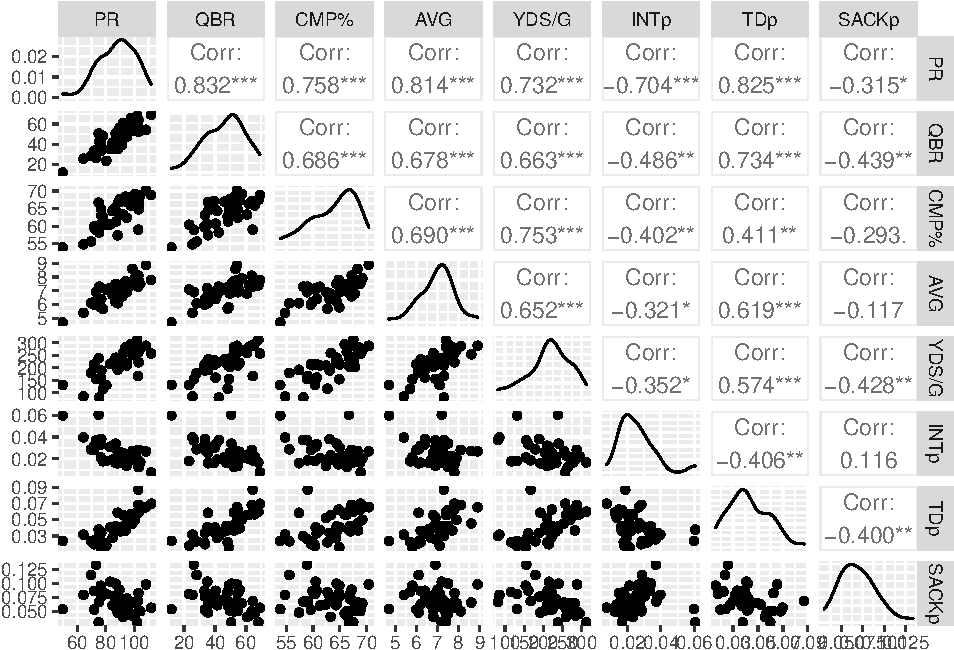
\includegraphics{textbook_files/figure-latex/unnamed-chunk-22-1.pdf}

\begin{enumerate}
\def\labelenumi{(\alph{enumi})}
\setcounter{enumi}{2}
\tightlist
\item
  What rate statistics are most correlated with passer efficiency and with QBR? Use CMP\% (completion percentage, completions per attempt), AVG (average yards per attempt), YDS/G (yards per game), and create new variables for interceptions per attempt, touchdowns per attempt, and sacks per attempt.
\end{enumerate}

\begin{Shaded}
\begin{Highlighting}[]
\CommentTok{\# Grab the counting statistics and create a correlation plot with PR and QBR}
\NormalTok{QB\_21 }\OtherTok{\textless{}{-}}\NormalTok{ QB\_21 }\SpecialCharTok{\%\textgreater{}\%} 
  \FunctionTok{mutate}\NormalTok{(}\AttributeTok{INTp =}\NormalTok{ INT}\SpecialCharTok{/}\NormalTok{ATT) }\SpecialCharTok{\%\textgreater{}\%}
  \FunctionTok{mutate}\NormalTok{(}\AttributeTok{TDp =}\NormalTok{ TD}\SpecialCharTok{/}\NormalTok{ATT) }\SpecialCharTok{\%\textgreater{}\%}
  \FunctionTok{mutate}\NormalTok{(}\AttributeTok{SACKp =}\NormalTok{ SACK}\SpecialCharTok{/}\NormalTok{ATT)}

\NormalTok{QB\_21 }\SpecialCharTok{\%\textgreater{}\%} \FunctionTok{select}\NormalTok{(PR,QBR,}\StringTok{\textasciigrave{}}\AttributeTok{CMP\%}\StringTok{\textasciigrave{}}\NormalTok{,AVG,}\StringTok{\textasciigrave{}}\AttributeTok{YDS/G}\StringTok{\textasciigrave{}}\NormalTok{,INTp,TDp,SACKp) }\SpecialCharTok{\%\textgreater{}\%} \FunctionTok{ggpairs}\NormalTok{()}
\end{Highlighting}
\end{Shaded}

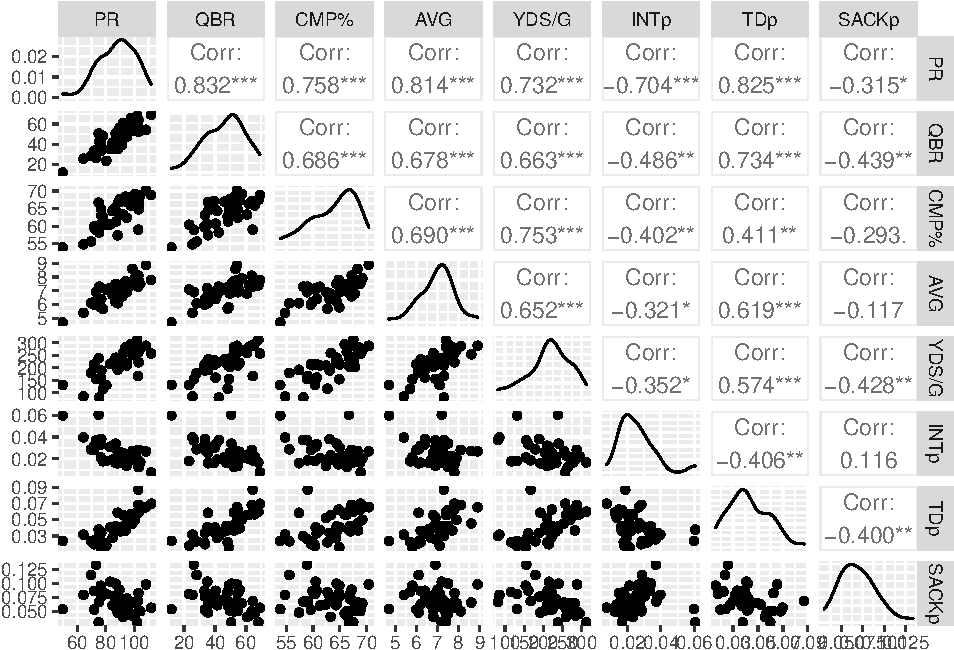
\includegraphics{textbook_files/figure-latex/unnamed-chunk-23-1.pdf}

\newpage

\hypertarget{basketball}{%
\section{Basketball}\label{basketball}}

\href{https://www.youtube.com/watch?v=wYjp2zoqQrs}{Link to YouTube video describing basketball rules}

\hypertarget{basic-basketball-statistics}{%
\subsection{Basic Basketball Statistics}\label{basic-basketball-statistics}}

\begin{itemize}
\item
  \textbf{Field Goal (FG)}: A made shot from either 2- or 3-point range. Free throws, worth 1 point, are not considered field goals. Field goal statistics often include attempts, makes, and percentage.
\item
  \textbf{Free Throw (FT)}: After certain fouls, the clock stops and a player shoots an uncontested shot from the foul line. These free throws are worth 1 point each; like with field goals, FT statistics often include attempts, makes, and percentage.
\item
  \textbf{Assists (AST)}: A player is credited with an assist if they pass the ball to a teammate and the teammate scores a field goal after zero or one dribbles. No more than one assist can be recorded per field goal.
\item
  \textbf{Turnover (TO)}: A player or team can be charged with a turnover for an action or violation that ends their offensive possession before being able to attempt a field goal. For a player (especially a guard), TOs can be compared to assists using Assist:Turnover ratio.
\item
  \textbf{Rebound (REB)}: The first player to gain control of the ball following a missed field goal is credited with a rebound. If the player is on the same team as the field goal shooter, it is an offensive rebound; otherwise, a defensive rebound.
\item
  \textbf{Points per Possession (PPP)}: Divides a team's points by number of possessions to account for a team's pace.
\end{itemize}

\hypertarget{advanced-basketball-statistics}{%
\subsection{Advanced Basketball Statistics}\label{advanced-basketball-statistics}}

\begin{itemize}
\item
  \textbf{True Shooting Percentage (TS\%)}: Unlike traditional shooting percentage, this statistic considers both field goals and free throws. It also gives more weight to shots that are worth more points.
\item
  \textbf{Win Shares}: Win shares give each player points for actions that contribute to a team's success. Win shares take into account a variety of offensive and defensive statistics, but can be calculated using different methods on different platforms.
\item
  \textbf{Value Over Replacement Player (VORP)}: This is basketball's response to baseball's WAR. VORP is a rate statistic that estimates a player's offensive output as compared to an ``average'' player.
\item
  \textbf{Player Efficiency Rating (PER)}: According to its creator John Hollinger,
  ``The PER sums up all a player's positive accomplishments, subtracts the negative accomplishments, and returns a per-minute rating of a player's performance.'' This statistic rewards great offensive performance more than great defensive plays.
\end{itemize}

\emph{References:}\\
\url{https://www.basketball-reference.com/about/per.html}\strut \\
\url{https://www.basketball-reference.com/about/ws.html}\strut \\
\url{https://www.basketball-reference.com/about/glossary.html}

\hypertarget{four-factors}{%
\subsection{Four Factors}\label{four-factors}}

Tibbles are a type of data frame supported by the \texttt{tidyverse} package. The following tibble contains data from a Mountain West tournament game played between the CSU and Wyoming women's basketball teams during the 2021-2022 season, which CSU won 51-38. \href{https://csurams.com/sports/womens-basketball/stats/2021-22/wyoming/boxscore/16095}{(Here's the link to the box score on the CSU athletics website.)}

\begin{Shaded}
\begin{Highlighting}[]
\NormalTok{basketball\_data }\OtherTok{\textless{}{-}} \FunctionTok{tibble}\NormalTok{(}\AttributeTok{team =} \FunctionTok{c}\NormalTok{(}\StringTok{"CSU"}\NormalTok{,}\StringTok{"WYO"}\NormalTok{), }\AttributeTok{FG =} \FunctionTok{c}\NormalTok{(}\DecValTok{14}\NormalTok{,}\DecValTok{15}\NormalTok{), }\AttributeTok{FGA =} \FunctionTok{c}\NormalTok{(}\DecValTok{48}\NormalTok{,}\DecValTok{60}\NormalTok{), }\AttributeTok{THREEP =} \FunctionTok{c}\NormalTok{(}\DecValTok{5}\NormalTok{,}\DecValTok{4}\NormalTok{), }\AttributeTok{FT =} \FunctionTok{c}\NormalTok{(}\DecValTok{10}\NormalTok{,}\DecValTok{4}\NormalTok{), }\AttributeTok{FTA =} \FunctionTok{c}\NormalTok{(}\DecValTok{14}\NormalTok{,}\DecValTok{4}\NormalTok{), }\AttributeTok{ORB =} \FunctionTok{c}\NormalTok{(}\DecValTok{2}\NormalTok{,}\DecValTok{14}\NormalTok{), }\AttributeTok{DRB =} \FunctionTok{c}\NormalTok{(}\DecValTok{31}\NormalTok{,}\DecValTok{30}\NormalTok{), }\AttributeTok{TOV =} \FunctionTok{c}\NormalTok{(}\DecValTok{5}\NormalTok{,}\DecValTok{12}\NormalTok{))}
\NormalTok{basketball\_data }\SpecialCharTok{\%\textgreater{}\%} \FunctionTok{kt}\NormalTok{()}
\end{Highlighting}
\end{Shaded}

\begin{table}[H]
\centering
\begin{tabular}{l|c|c|c|c|c|c|c|c}
\hline
team & FG & FGA & THREEP & FT & FTA & ORB & DRB & TOV\\
\hline
CSU & 14 & 48 & 5 & 10 & 14 & 2 & 31 & 5\\
\hline
WYO & 15 & 60 & 4 & 4 & 4 & 14 & 30 & 12\\
\hline
\end{tabular}
\end{table}

This tibble contains all the data needed to calculate the \emph{Four Factors}. The Four Factors of a basketball game are statistics formulated by Dean Oliver, former Director of Quantitative Analysis for the Denver Nuggets (among other roles). These statistics are also promoted by sports data platforms like Hudl.com.

The Four Factors each have offensive and defensive versions; for this example, we'll focus on the offensive perspective.

\begin{enumerate}
\def\labelenumi{\arabic{enumi}.}
\tightlist
\item
  \textbf{\emph{Scoring}}: \textbf{Effective Field Goal Percentage} (eFG\%)
\end{enumerate}

\(eFG\% = \frac{FG\ +\ 0.5(3P)}{FGA}\)

\begin{enumerate}
\def\labelenumi{\arabic{enumi}.}
\setcounter{enumi}{1}
\tightlist
\item
  \textbf{\emph{Crashing}}: \textbf{Turnover Percentage} (TOV\%)
\end{enumerate}

\(TOV\% = \frac{TOV}{FGA\ +\ 0.44(FTA)\ +\ TOV}\)

\begin{enumerate}
\def\labelenumi{\arabic{enumi}.}
\setcounter{enumi}{2}
\tightlist
\item
  \textbf{\emph{Protecting}}: \textbf{Rebounding Percentage} (ORB\%)
\end{enumerate}

\(ORB\% = \frac{ORB}{ORB\ +\ Opponent\ DRB}\)

\begin{enumerate}
\def\labelenumi{\arabic{enumi}.}
\setcounter{enumi}{3}
\tightlist
\item
  \textbf{\emph{Attacking}}: \textbf{Free Throw Factor} (FT Factor)
\end{enumerate}

\(FT\ factor = \frac{FT}{FGA}\)

Let's calculate the values of eFG\%, TOV\%, ORB\%, and Free Throw Factor for both CSU and Wyoming and add them as new columns in the tibble using the \texttt{add\_column} function.

\begin{Shaded}
\begin{Highlighting}[]
\NormalTok{basketball\_data }\OtherTok{\textless{}{-}}\NormalTok{ basketball\_data }\SpecialCharTok{\%\textgreater{}\%} 
  \FunctionTok{mutate}\NormalTok{(}\AttributeTok{eFG =} \DecValTok{100}\SpecialCharTok{*}\NormalTok{(FG }\SpecialCharTok{+}\NormalTok{ .}\DecValTok{5} \SpecialCharTok{*}\NormalTok{ THREEP)}\SpecialCharTok{/}\NormalTok{FGA) }\SpecialCharTok{\%\textgreater{}\%}
  \FunctionTok{mutate}\NormalTok{(}\AttributeTok{TOVPCT =} \DecValTok{100}\SpecialCharTok{*}\NormalTok{(FG }\SpecialCharTok{+}\NormalTok{ .}\DecValTok{5} \SpecialCharTok{*}\NormalTok{ THREEP)}\SpecialCharTok{/}\NormalTok{FGA) }\SpecialCharTok{\%\textgreater{}\%}
  \FunctionTok{mutate}\NormalTok{(}\AttributeTok{ORBPCT =} \DecValTok{100}\SpecialCharTok{*}\FunctionTok{c}\NormalTok{(ORB[}\DecValTok{1}\NormalTok{]}\SpecialCharTok{/}\NormalTok{(ORB[}\DecValTok{1}\NormalTok{]}\SpecialCharTok{+}\NormalTok{DRB[}\DecValTok{2}\NormalTok{]), ORB[}\DecValTok{2}\NormalTok{]}\SpecialCharTok{/}\NormalTok{(ORB[}\DecValTok{2}\NormalTok{]}\SpecialCharTok{+}\NormalTok{DRB[}\DecValTok{1}\NormalTok{]))) }\SpecialCharTok{\%\textgreater{}\%}
  \FunctionTok{mutate}\NormalTok{(}\AttributeTok{FTFACTOR =} \DecValTok{100}\SpecialCharTok{*}\NormalTok{FT}\SpecialCharTok{/}\NormalTok{FGA)}

\NormalTok{basketball\_data }\SpecialCharTok{\%\textgreater{}\%} \FunctionTok{select}\NormalTok{(team,eFG, TOVPCT, ORBPCT, FTFACTOR) }\SpecialCharTok{\%\textgreater{}\%} \FunctionTok{kt}\NormalTok{()}
\end{Highlighting}
\end{Shaded}

\begin{table}[H]
\centering
\begin{tabular}{l|c|c|c|c}
\hline
team & eFG & TOVPCT & ORBPCT & FTFACTOR\\
\hline
CSU & 34.375 & 34.375 & 6.250 & 20.833\\
\hline
WYO & 28.333 & 28.333 & 31.111 & 6.667\\
\hline
\end{tabular}
\end{table}

While this method does produce Four Factors data, it could be difficult to scale for calculating the same statistics for a sample of several games. In the next section, we will introduce an \texttt{R} package that aids in the calculation of Four Factors.

\hypertarget{basketballanalyzer-four-factors}{%
\subsubsection{BasketballAnalyzeR Four Factors}\label{basketballanalyzer-four-factors}}

The authors of ``Basketball Data Science With Applications in R'' developed the \texttt{BasketballAnalyzeR} package to be used in conjunction with the book. \texttt{BasketballAnalyzeR} includes built-in datasets from the 2017-18 NBA season and provides many functions for analyzing and plotting basketball data. One such function is \texttt{fourfactors}, which offers a simpler way to perform a four factors analysis.

\begin{Shaded}
\begin{Highlighting}[]
\FunctionTok{library}\NormalTok{(}\StringTok{"BasketballAnalyzeR"}\NormalTok{)}

\NormalTok{teams }\OtherTok{\textless{}{-}} \FunctionTok{c}\NormalTok{(}\StringTok{"DEN"}\NormalTok{, }\StringTok{"CLE"}\NormalTok{, }\StringTok{"GSW"}\NormalTok{) }\CommentTok{\#Nuggets, Cavaliers, Warriors}
\NormalTok{team\_data }\OtherTok{\textless{}{-}} \FunctionTok{which}\NormalTok{(Tadd}\SpecialCharTok{$}\NormalTok{team }\SpecialCharTok{\%in\%}\NormalTok{ teams)}
\NormalTok{four\_factors\_teams }\OtherTok{\textless{}{-}} \FunctionTok{fourfactors}\NormalTok{(Tbox[team\_data, ], Obox[team\_data, ])}
\NormalTok{four\_factors\_teams }\SpecialCharTok{\%\textgreater{}\%} \FunctionTok{select}\NormalTok{(}\DecValTok{1}\NormalTok{,}\DecValTok{8}\SpecialCharTok{:}\DecValTok{15}\NormalTok{) }\SpecialCharTok{\%\textgreater{}\%} \FunctionTok{kt}\NormalTok{()}
\end{Highlighting}
\end{Shaded}

\begin{table}[H]
\centering
\begin{tabular}{l|c|c|c|c|c|c|c|c}
\hline
Team & F1.Off & F2.Off & F3.Off & F4.Off & F1.Def & F2.Def & F3.Def & F4.Def\\
\hline
Cleveland Cavaliers & 54.70 & 13.70 & 20.06 & 21.41 & 53.98 & 13.43 & 77.27 & 16.58\\
\hline
Denver Nuggets & 53.62 & 14.90 & 25.66 & 19.77 & 53.88 & 13.83 & 77.45 & 17.35\\
\hline
Golden State Warriors & 56.91 & 15.26 & 21.05 & 19.48 & 50.44 & 13.89 & 76.31 & 18.55\\
\hline
\end{tabular}
\end{table}

This is a much simpler and neater way to calculate Four Factors.

In the 2017-18 season, the Warriors and Cavaliers met in the NBA Finals, while the Nuggets just missed the playoffs. It would be expected that the two Finals teams would have higher values for the Four Factors. While this is mostly true, for which of the Four Factors did the Nuggets have the highest value?

A: Factor 3 (rebounding percentage), both offensive and defensive.

\hypertarget{shot-charts}{%
\subsection{Shot Charts}\label{shot-charts}}

The \texttt{BasketballAnalyzeR} package includes shot location data for all players for the 2017-18 NBA season and has a function called \texttt{shotchart} that allows for the plotting of shot data.

Let's plot shot location data for Nikola Jokic. First, the coordinates must be transformed so that the point (0,0) is located at the corner of the court; the original coordinates place the origin at the center of the hoop.

\begin{Shaded}
\begin{Highlighting}[]
\NormalTok{PbP }\OtherTok{\textless{}{-}} \FunctionTok{PbPmanipulation}\NormalTok{(PbP.BDB)}

\NormalTok{jokic\_data }\OtherTok{\textless{}{-}} \FunctionTok{subset}\NormalTok{(PbP, player }\SpecialCharTok{==} \StringTok{"Nikola Jokic"}\NormalTok{)}
\NormalTok{jokic\_data}\SpecialCharTok{$}\NormalTok{xx }\OtherTok{\textless{}{-}}\NormalTok{ jokic\_data}\SpecialCharTok{$}\NormalTok{original\_x}\SpecialCharTok{/}\DecValTok{10} \CommentTok{\#transformation}
\NormalTok{jokic\_data}\SpecialCharTok{$}\NormalTok{yy }\OtherTok{\textless{}{-}}\NormalTok{ jokic\_data}\SpecialCharTok{$}\NormalTok{original\_y}\SpecialCharTok{/}\DecValTok{10} \SpecialCharTok{{-}} \FloatTok{41.75} \CommentTok{\#transformation}
\end{Highlighting}
\end{Shaded}

\texttt{BasketballAnalyzeR} supports three types of density visualizations within \texttt{shotchart}, one being \texttt{density-polygons}. Since \texttt{shotchart} is a \texttt{ggplot} object, a chart title can be added using \texttt{ggtitle}.

\begin{Shaded}
\begin{Highlighting}[]
\FunctionTok{shotchart}\NormalTok{(}\AttributeTok{data =}\NormalTok{ jokic\_data, }\AttributeTok{x=}\StringTok{"xx"}\NormalTok{, }\AttributeTok{y=}\StringTok{"yy"}\NormalTok{, }\AttributeTok{type=}\StringTok{"density{-}polygons"}\NormalTok{) }\SpecialCharTok{+} \FunctionTok{ggtitle}\NormalTok{(}\StringTok{"Nikola Jokic Shot Data, 2017{-}18"}\NormalTok{)}
\end{Highlighting}
\end{Shaded}

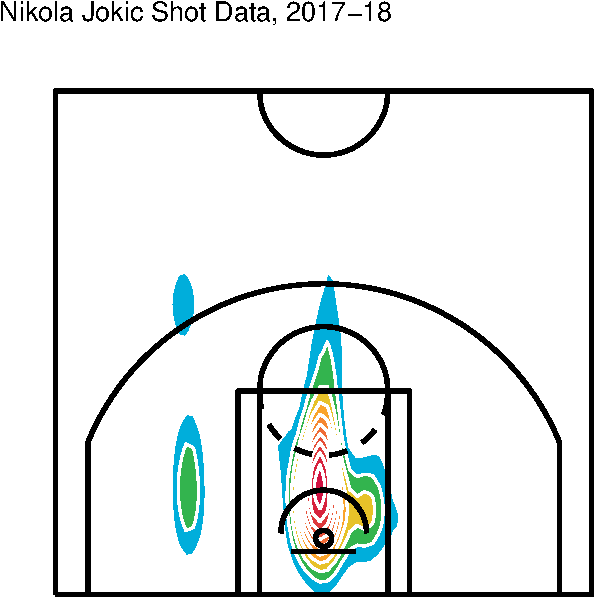
\includegraphics{textbook_files/figure-latex/basketballanalyzer 3-1.pdf}

It seems most shots attempts from Jokic were in the paint; this is hardly surprising, since he plays the center position. Here's the same chart with \texttt{density-hexbin}:

\begin{Shaded}
\begin{Highlighting}[]
\FunctionTok{shotchart}\NormalTok{(}\AttributeTok{data =}\NormalTok{ jokic\_data, }\AttributeTok{x=}\StringTok{"xx"}\NormalTok{, }\AttributeTok{y=}\StringTok{"yy"}\NormalTok{, }\AttributeTok{type=}\StringTok{"density{-}hexbin"}\NormalTok{) }\SpecialCharTok{+} \FunctionTok{ggtitle}\NormalTok{(}\StringTok{"Nikola Jokic Shot Data, 2017{-}18"}\NormalTok{)}
\end{Highlighting}
\end{Shaded}

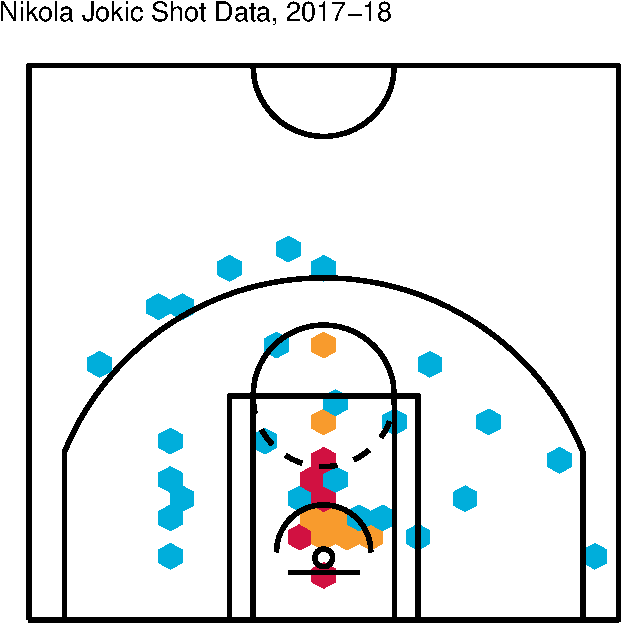
\includegraphics{textbook_files/figure-latex/basketballanalyzer 4-1.pdf}

The same chart with \texttt{density-raster}:

\begin{Shaded}
\begin{Highlighting}[]
\FunctionTok{shotchart}\NormalTok{(}\AttributeTok{data =}\NormalTok{ jokic\_data, }\AttributeTok{x=}\StringTok{"xx"}\NormalTok{, }\AttributeTok{y=}\StringTok{"yy"}\NormalTok{, }\AttributeTok{type=}\StringTok{"density{-}raster"}\NormalTok{) }\SpecialCharTok{+} \FunctionTok{ggtitle}\NormalTok{(}\StringTok{"Nikola Jokic Shot Data, 2017{-}18"}\NormalTok{)}
\end{Highlighting}
\end{Shaded}

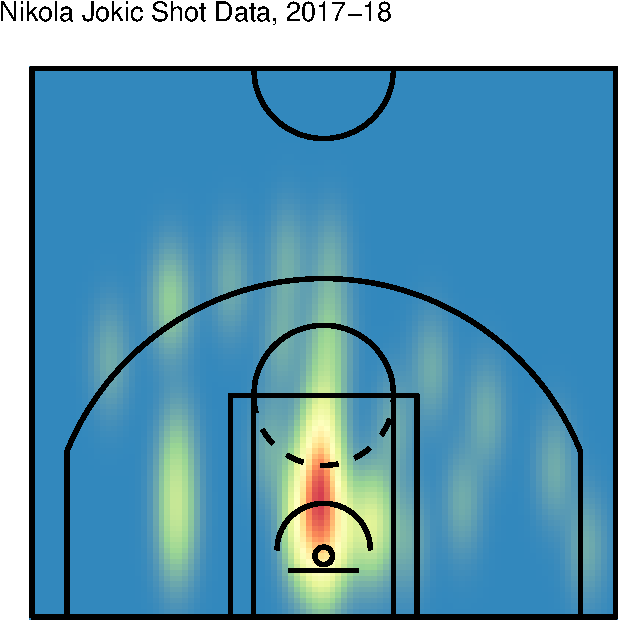
\includegraphics{textbook_files/figure-latex/basketballanalyzer 5-1.pdf}

Within the \texttt{shotchart} function, setting \texttt{scatter=TRUE} overlays the shots on the chart. Point size and transparency can also be customized.

\begin{Shaded}
\begin{Highlighting}[]
\FunctionTok{shotchart}\NormalTok{(}\AttributeTok{data =}\NormalTok{ jokic\_data, }\AttributeTok{x=}\StringTok{"xx"}\NormalTok{, }\AttributeTok{y=}\StringTok{"yy"}\NormalTok{, }\AttributeTok{type=}\StringTok{"density{-}raster"}\NormalTok{, }\AttributeTok{scatter=}\ConstantTok{TRUE}\NormalTok{) }\SpecialCharTok{+} \FunctionTok{ggtitle}\NormalTok{(}\StringTok{"Nikola Jokic Shot Data, 2017{-}18"}\NormalTok{)}
\end{Highlighting}
\end{Shaded}

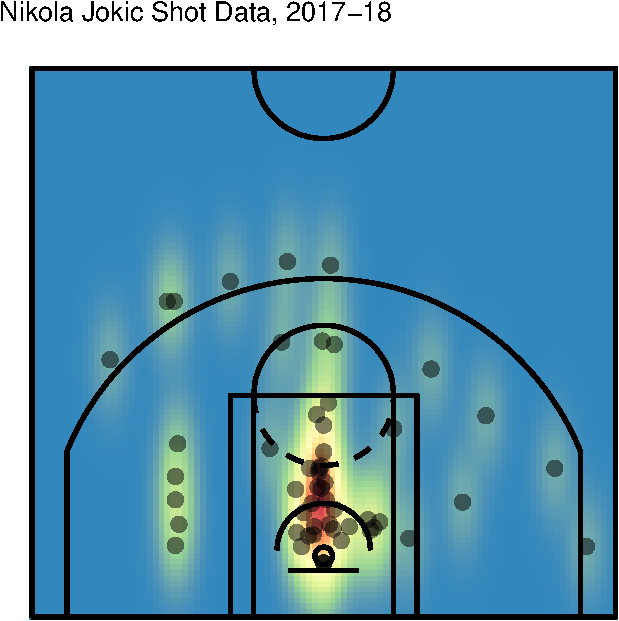
\includegraphics{textbook_files/figure-latex/basketballanalyzer 6-1.pdf}

Let's now compare shot charts of Nikola Jokic, Steph Curry, and Lebron James. This group of players includes one member of each team for which we calculated Four Factors.

\begin{Shaded}
\begin{Highlighting}[]
\NormalTok{curry\_data }\OtherTok{\textless{}{-}} \FunctionTok{subset}\NormalTok{(PbP, player }\SpecialCharTok{==} \StringTok{"Stephen Curry"}\NormalTok{)}
\NormalTok{curry\_data}\SpecialCharTok{$}\NormalTok{xx }\OtherTok{\textless{}{-}}\NormalTok{ curry\_data}\SpecialCharTok{$}\NormalTok{original\_x}\SpecialCharTok{/}\DecValTok{10} \CommentTok{\#transformation}
\NormalTok{curry\_data}\SpecialCharTok{$}\NormalTok{yy }\OtherTok{\textless{}{-}}\NormalTok{ curry\_data}\SpecialCharTok{$}\NormalTok{original\_y}\SpecialCharTok{/}\DecValTok{10} \SpecialCharTok{{-}} \FloatTok{41.75} \CommentTok{\#transformation}

\NormalTok{james\_data }\OtherTok{\textless{}{-}} \FunctionTok{subset}\NormalTok{(PbP, player }\SpecialCharTok{==} \StringTok{"LeBron James"}\NormalTok{)}
\NormalTok{james\_data}\SpecialCharTok{$}\NormalTok{xx }\OtherTok{\textless{}{-}}\NormalTok{ james\_data}\SpecialCharTok{$}\NormalTok{original\_x}\SpecialCharTok{/}\DecValTok{10} \CommentTok{\#transformation}
\NormalTok{james\_data}\SpecialCharTok{$}\NormalTok{yy }\OtherTok{\textless{}{-}}\NormalTok{ james\_data}\SpecialCharTok{$}\NormalTok{original\_y}\SpecialCharTok{/}\DecValTok{10} \SpecialCharTok{{-}} \FloatTok{41.75} \CommentTok{\#transformation}

\FunctionTok{shotchart}\NormalTok{(}\AttributeTok{data =}\NormalTok{ jokic\_data, }\AttributeTok{x=}\StringTok{"xx"}\NormalTok{, }\AttributeTok{y=}\StringTok{"yy"}\NormalTok{, }\AttributeTok{type=}\StringTok{"density{-}raster"}\NormalTok{) }\SpecialCharTok{+} \FunctionTok{ggtitle}\NormalTok{(}\StringTok{"Nikola Jokic Shot Data, 2017{-}18"}\NormalTok{)}
\end{Highlighting}
\end{Shaded}

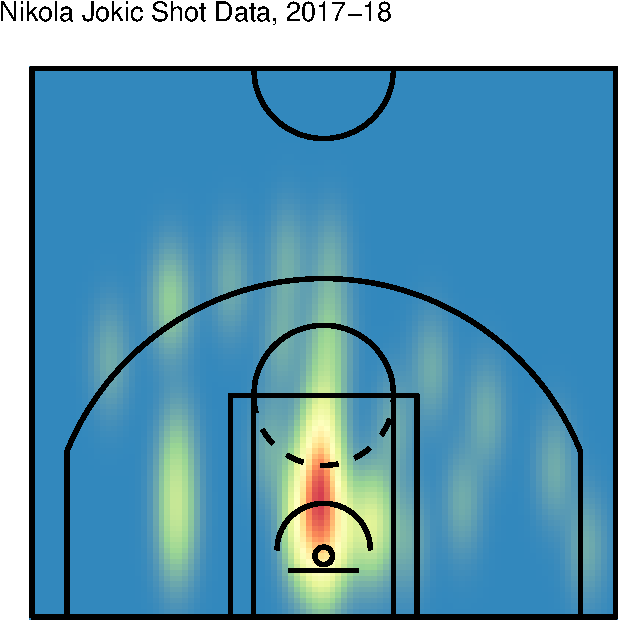
\includegraphics{textbook_files/figure-latex/basketballanalyzer 7-1.pdf}

\begin{Shaded}
\begin{Highlighting}[]
\FunctionTok{shotchart}\NormalTok{(}\AttributeTok{data =}\NormalTok{ curry\_data, }\AttributeTok{x=}\StringTok{"xx"}\NormalTok{, }\AttributeTok{y=}\StringTok{"yy"}\NormalTok{, }\AttributeTok{type=}\StringTok{"density{-}raster"}\NormalTok{) }\SpecialCharTok{+} \FunctionTok{ggtitle}\NormalTok{(}\StringTok{"Steph Curry Shot Data, 2017{-}18"}\NormalTok{)}
\end{Highlighting}
\end{Shaded}

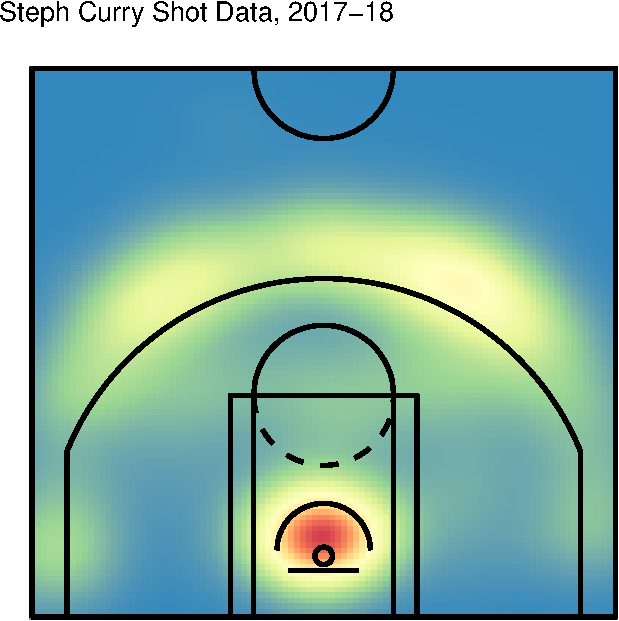
\includegraphics{textbook_files/figure-latex/basketballanalyzer 7-2.pdf}

\begin{Shaded}
\begin{Highlighting}[]
\FunctionTok{shotchart}\NormalTok{(}\AttributeTok{data =}\NormalTok{ james\_data, }\AttributeTok{x=}\StringTok{"xx"}\NormalTok{, }\AttributeTok{y=}\StringTok{"yy"}\NormalTok{, }\AttributeTok{type=}\StringTok{"density{-}raster"}\NormalTok{) }\SpecialCharTok{+} \FunctionTok{ggtitle}\NormalTok{(}\StringTok{"Lebron James Shot Data, 2017{-}18"}\NormalTok{)}
\end{Highlighting}
\end{Shaded}

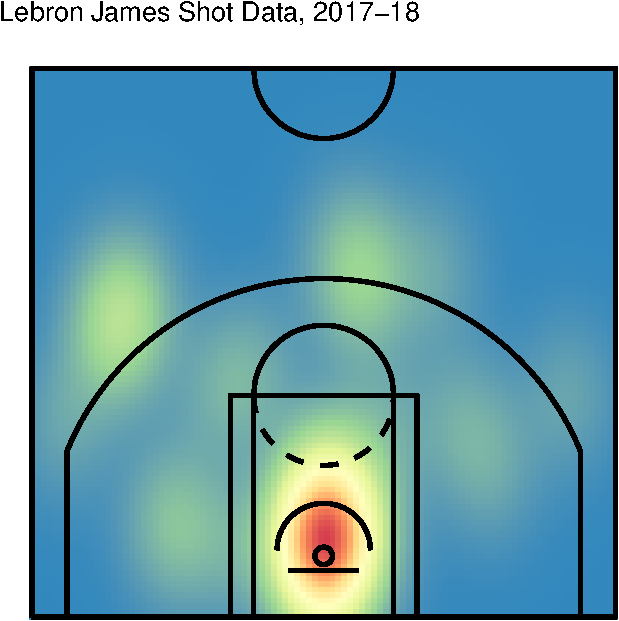
\includegraphics{textbook_files/figure-latex/basketballanalyzer 7-3.pdf}

Q: Of the three players (Jokic, Curry, James), which took the highest percentage of their three-point shots from the right side of the court (when facing the basket)?

A: Nikola Jokic shot almost all of his attempts from the right side. Steph Curry took many shots from beyond the arc and tended toward the left side, while James was split between the right side and the center.

Now, let's focus on Steph Curry's shooting. The following chart splits the court into zones based on angle and distance from the basket. The color in each zone represents the average length of the play leading up to that shot among shots taken in that zone.

\begin{Shaded}
\begin{Highlighting}[]
\FunctionTok{shotchart}\NormalTok{(}\AttributeTok{data =}\NormalTok{ curry\_data, }\AttributeTok{x=}\StringTok{"xx"}\NormalTok{, }\AttributeTok{y=}\StringTok{"yy"}\NormalTok{, }\AttributeTok{z=}\StringTok{"playlength"}\NormalTok{, }\AttributeTok{type=}\StringTok{"sectors"}\NormalTok{, }\AttributeTok{num.sect =} \DecValTok{7}\NormalTok{, }\AttributeTok{scatter=}\ConstantTok{TRUE}\NormalTok{, }\AttributeTok{pt.alpha=}\NormalTok{.}\DecValTok{3}\NormalTok{) }\SpecialCharTok{+} \FunctionTok{ggtitle}\NormalTok{(}\StringTok{"Steph Curry Shot Data, 2017{-}18"}\NormalTok{)}
\end{Highlighting}
\end{Shaded}

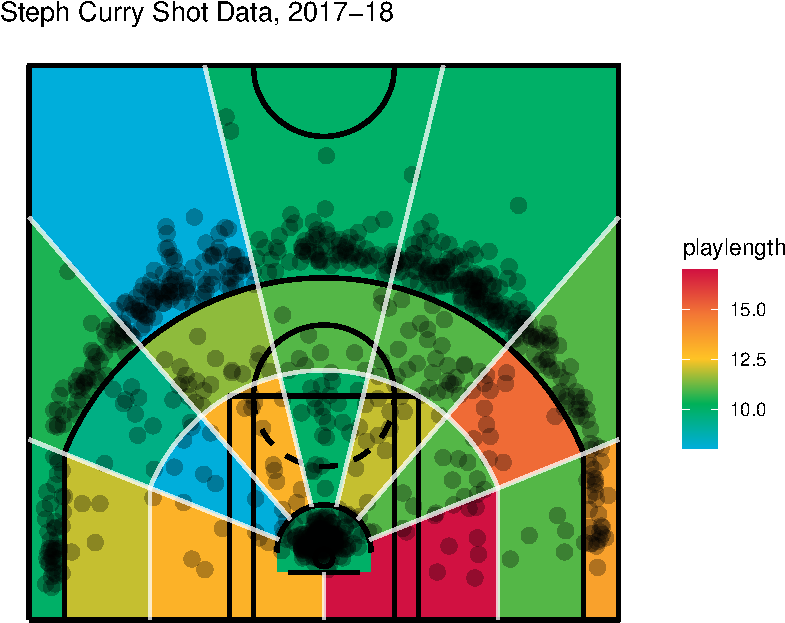
\includegraphics{textbook_files/figure-latex/basketballanalyzer 8-1.pdf}

Q: In general, did Steph Curry tend to shoot closer to the basket during plays of a longer duration or a shorter duration?

A: There is not a perfect correlation, but it seems that two-point field goals were attempted more often during longer plays, while shots taken outside the three-point arc were taken during plays of a shorter duration.

\emph{References:}
\url{https://rdrr.io/cran/BasketballAnalyzeR/}\\
Basketball Data Science (Zuccolotto and Manisera, 2020)

\newpage

\hypertarget{hockey}{%
\section{Hockey}\label{hockey}}

\href{https://www.youtube.com/watch?v=nv2FUnHceqU}{Link to YouTube video describing hockey rules}

\hypertarget{basic-hockey-statistics}{%
\subsection{Basic Hockey Statistics}\label{basic-hockey-statistics}}

Here are some basic statistics that are used often to describe hockey games.

\begin{itemize}
\item
  \textbf{Goals (G)}: If a team scores, the skater on the scoring team who last touched the puck is credited with a goal.
\item
  \textbf{Assists (A)}: The players (up to two) on the scoring team who last touch the puck before the goalscorer are credited with assists, unless the opposing team has possession of the puck in between.
\item
  \textbf{Points (PTS)}: Goals plus assists. {[}Not to be confused with team points awarded in the regular season standings by the many hockey leagues, including the NHL (two points for a win, one point for an overtime/shootout loss, zero points for a regulation loss){]}.
\item
  \textbf{Shots On Goal (SOG)}: Shot attempts in which the puck has been shot directly on goal. Shot attempts which are blocked or miss the goal are not considered SOGs. A team's shots on goal should equal the opposing goaltender's saves plus the team's goals scored.
\item
  \textbf{Goals Against Average (GAA)}: Of a goaltender, the number of goals allowed by that goaltender adjusted to a per-60 minute rate.
\item
  \textbf{Penalty Minutes (PIM)}: The amount of penalty time an individual player is assigned for their infractions. PIM may be different than the amount of time the player actually spends in the penalty box.
\end{itemize}

\emph{Reference:}\\
\url{https://www.milehighhockey.com/pages/stats}

\hypertarget{advanced-hockey-statistics}{%
\subsection{Advanced Hockey Statistics}\label{advanced-hockey-statistics}}

\begin{itemize}
\item
  \textbf{CORSI}: CORSI only applies to 5 on 5 (``even-strength'') situations. It is calculated as the difference between shot attempts on offense (shots on goal + blocked shots + missed shots) minus shot attempts allowed on defense. CORSI can also be expressed as a percentage, with percentages over 50\% indicating that the player is on ice for more offensive shots than defensive shots.
\item
  \textbf{Expected Goals (xG)}: Expected Goals statistics give each shot an estimated probability of scoring a goal based on factors such as shot location and game situation. xG cannot be less than 0 or greater than 1 for any particular shot, and different platforms may have different methods of calculating expected goals.
\item
  \textbf{Fenwick/Unblocked Shot Attempts (USAT)}: Similar to CORSI, but omits blocked shots from the calculation. This statistic is used in many Expected Goals calculations.
\end{itemize}

Because the flow of a hockey game is usually quite different in situations other than the normal 5 on 5, such as a power play (5 on 4) or concurrent penalties (4 on 4), many hockey databases separate data by the type of game situation. We will see this below with a dataset from \href{www.moneypuck.com}{MoneyPuck}, but it is also present on \href{https://www.naturalstattrick.com/}{Natural Stat Trick}, \href{www.quanthockey.com}{QuantHockey}, and \href{www.hockey-reference.com}{hockey-reference}.

\emph{References:}\\
\url{https://www.nhl.com/lightning/news/hockey-analytics-101-understanding-advanced-stats-and-how-theyre-measured/c-735819}\strut \\
\url{https://theathletic.com/121980/2017/10/09/an-advanced-stat-primer-understanding-basic-hockey-metrics/}

\hypertarget{actual-vs.-expected-goals}{%
\subsection{Actual vs.~Expected Goals}\label{actual-vs.-expected-goals}}

\begin{example}
For this example, we'll use a set of NHL data from moneypuck.com. First, let's load the data into \texttt{R} and open the data frame.
\end{example}

\begin{Shaded}
\begin{Highlighting}[]
\NormalTok{nhl\_2022\_data }\OtherTok{\textless{}{-}} \FunctionTok{read\_csv}\NormalTok{(}\StringTok{"https://moneypuck.com/moneypuck/playerData/seasonSummary/2021/regular/teams.csv"}\NormalTok{)}

\NormalTok{nhl\_2022\_data }\SpecialCharTok{\%\textgreater{}\%} \FunctionTok{slice\_head}\NormalTok{(}\AttributeTok{n=}\DecValTok{10}\NormalTok{) }\SpecialCharTok{\%\textgreater{}\%} \FunctionTok{select}\NormalTok{(}\DecValTok{3}\NormalTok{,}\DecValTok{6}\NormalTok{,}\DecValTok{8}\NormalTok{,}\DecValTok{9}\NormalTok{,}\DecValTok{10}\NormalTok{) }\SpecialCharTok{\%\textgreater{}\%} \FunctionTok{kt}\NormalTok{()}
\end{Highlighting}
\end{Shaded}

\begin{table}[H]
\centering
\begin{tabular}{l|c|c|c|c}
\hline
name & situation & xGoalsPercentage & corsiPercentage & fenwickPercentage\\
\hline
WPG & other & 0.49 & 0.50 & 0.47\\
\hline
WPG & all & 0.49 & 0.50 & 0.50\\
\hline
WPG & 5on5 & 0.49 & 0.49 & 0.50\\
\hline
WPG & 4on5 & 0.16 & 0.14 & 0.15\\
\hline
WPG & 5on4 & 0.86 & 0.86 & 0.85\\
\hline
CBJ & other & 0.52 & 0.49 & 0.49\\
\hline
CBJ & all & 0.45 & 0.48 & 0.47\\
\hline
CBJ & 5on5 & 0.45 & 0.48 & 0.47\\
\hline
CBJ & 4on5 & 0.14 & 0.18 & 0.21\\
\hline
CBJ & 5on4 & 0.81 & 0.84 & 0.82\\
\hline
\end{tabular}
\end{table}

We can create nice looking tables using the ``kableExtra'\,' package. Let's look at the first eight rows and a small selection of columns of the data frame and format the table output using a kable table.

\begin{Shaded}
\begin{Highlighting}[]
\FunctionTok{library}\NormalTok{(}\StringTok{"kableExtra"}\NormalTok{)}

\NormalTok{nhl\_2022\_data[}\DecValTok{1}\SpecialCharTok{:}\DecValTok{8}\NormalTok{, }\FunctionTok{c}\NormalTok{(}\DecValTok{3}\NormalTok{,}\DecValTok{6}\SpecialCharTok{:}\DecValTok{9}\NormalTok{)] }\SpecialCharTok{\%\textgreater{}\%} \FunctionTok{kt}\NormalTok{()}
\end{Highlighting}
\end{Shaded}

\begin{table}[H]
\centering
\begin{tabular}{l|c|c|c|c}
\hline
name & situation & games\_played & xGoalsPercentage & corsiPercentage\\
\hline
WPG & other & 82 & 0.49 & 0.50\\
\hline
WPG & all & 82 & 0.49 & 0.50\\
\hline
WPG & 5on5 & 82 & 0.49 & 0.49\\
\hline
WPG & 4on5 & 82 & 0.16 & 0.14\\
\hline
WPG & 5on4 & 82 & 0.86 & 0.86\\
\hline
CBJ & other & 82 & 0.52 & 0.49\\
\hline
CBJ & all & 82 & 0.45 & 0.48\\
\hline
CBJ & 5on5 & 82 & 0.45 & 0.48\\
\hline
\end{tabular}
\end{table}

This dataset includes a \emph{lot} of covariates. It also splits these data by different game situations: even-strength (5 on 5), power play (5 on 4), etc. Let's subset the data to include all game situations.

Use the \texttt{nrow} command to check the number of columns in the new data frame. Check: Is it the same as the number of teams in the league for the 2021-2022 season?

\begin{Shaded}
\begin{Highlighting}[]
\NormalTok{nhl\_data\_all }\OtherTok{\textless{}{-}} \FunctionTok{filter}\NormalTok{(nhl\_2022\_data, situation }\SpecialCharTok{==} \StringTok{"all"}\NormalTok{)}

\FunctionTok{nrow}\NormalTok{(nhl\_data\_all)}
\end{Highlighting}
\end{Shaded}

\begin{verbatim}
## [1] 32
\end{verbatim}

The dataset includes an Expected Goals statistic for each team in the \texttt{xGoalsFor} column. Let's plot this quantity against the team's actual number of goals scored; this is given by the \texttt{goalsFor} column.

(Remember to always have a good title and axis labels!)

\begin{Shaded}
\begin{Highlighting}[]
\FunctionTok{ggplot}\NormalTok{(}\AttributeTok{data=}\NormalTok{nhl\_data\_all, }\FunctionTok{aes}\NormalTok{(}\AttributeTok{x=}\NormalTok{xGoalsFor, }\AttributeTok{y=}\NormalTok{goalsFor)) }\SpecialCharTok{+} \FunctionTok{labs}\NormalTok{(}\AttributeTok{x=}\StringTok{"Expected Goals Scored"}\NormalTok{, }\AttributeTok{y=}\StringTok{"Actual Goals Scored"}\NormalTok{, }\AttributeTok{title=}\StringTok{"NHL Teams: Expected vs. Actual Goals, 2021{-}22"}\NormalTok{) }\SpecialCharTok{+} \FunctionTok{geom\_point}\NormalTok{()}
\end{Highlighting}
\end{Shaded}

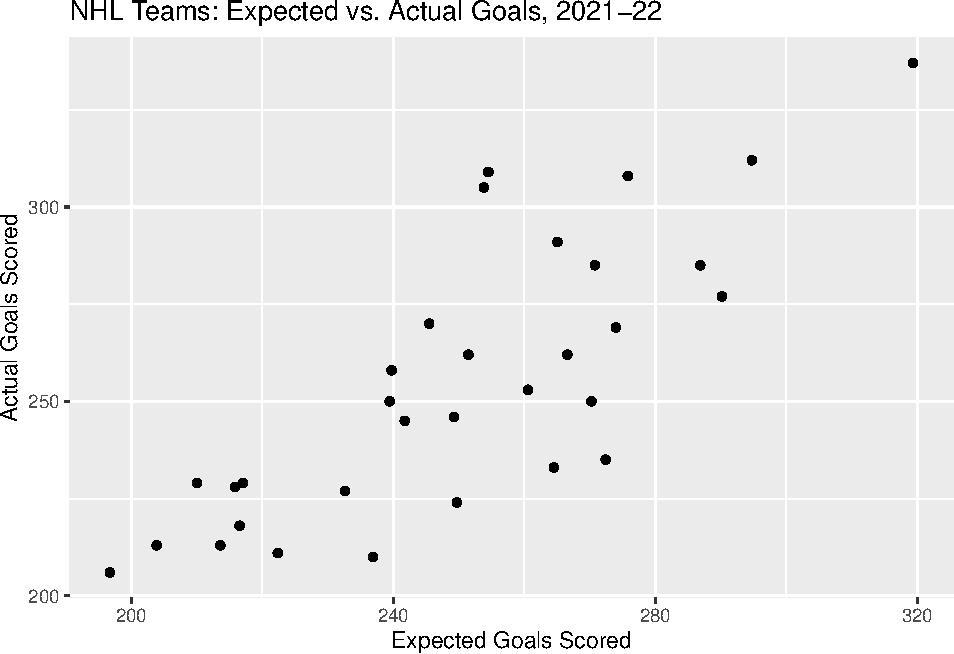
\includegraphics{textbook_files/figure-latex/unnamed-chunk-26-1.pdf}

As expected, there is a general positive correlation between expected and actual goals (\(r \approx 0.8\)). However, there is some variability - for example, the Kings only scored 7 more actual goals than the Ducks, despite having 56.6 more expected goals.

Let's add a line to the graph using the \texttt{geom\_abline} function corresponding to the line \(y=x\), the line on which data points would fall if expected goals were equal to actual goals. We can also customize the line's color and type.

\begin{Shaded}
\begin{Highlighting}[]
\FunctionTok{ggplot}\NormalTok{(}\AttributeTok{data=}\NormalTok{nhl\_data\_all, }\FunctionTok{aes}\NormalTok{(}\AttributeTok{x=}\NormalTok{xGoalsFor, }\AttributeTok{y=}\NormalTok{goalsFor)) }\SpecialCharTok{+} \FunctionTok{labs}\NormalTok{(}\AttributeTok{x=}\StringTok{"Expected Goals Scored"}\NormalTok{, }\AttributeTok{y=}\StringTok{"Actual Goals Scored"}\NormalTok{,}\AttributeTok{title=}\StringTok{"NHL Teams: Expected vs. Actual Goals, 2021{-}22"}\NormalTok{) }\SpecialCharTok{+} \FunctionTok{geom\_point}\NormalTok{() }\SpecialCharTok{+} \FunctionTok{geom\_abline}\NormalTok{(}\AttributeTok{intercept=}\DecValTok{0}\NormalTok{, }\AttributeTok{slope=}\DecValTok{1}\NormalTok{, }\AttributeTok{color=}\StringTok{"red"}\NormalTok{, }\AttributeTok{linetype=}\StringTok{"dashed"}\NormalTok{)}
\end{Highlighting}
\end{Shaded}

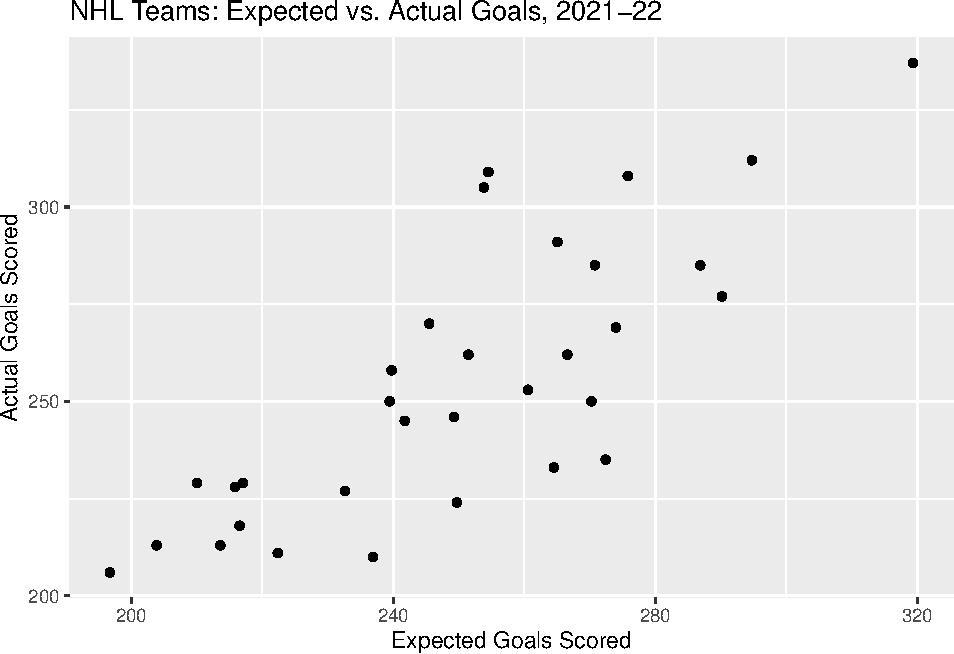
\includegraphics{textbook_files/figure-latex/unnamed-chunk-27-1.pdf}

\emph{Note: A slope of 0 and an intercept of 1 are actually the default parameters for the function.}

Q: What does it mean for a team's data point to fall below this line? Above it?

A: If the data point is below the line, it means the expected goals were greater than the actual goals; if the data point is above the line, it means the actual goals were greater than the expected goals.

Q: Do you think that a team's expected goals would be more likely to be closer to its actual goals for a ten-game stretch, an entire season, or five consecutive seasons? Why?

A: We would expect that as sample size increases, the result would become closer to expectation. So, actual goals would be most likely closer to expected goals over a span of five seasons.

\hypertarget{goalie-statistics}{%
\subsection{Goalie Statistics}\label{goalie-statistics}}

\begin{example}
For this next example, let's use goalie data from the 2021-2022 season from \href{https://www.naturalstattrick.com/}{Natural Stat Trick}.
\end{example}

\begin{Shaded}
\begin{Highlighting}[]
\NormalTok{goalie\_data }\OtherTok{\textless{}{-}} \FunctionTok{read.csv}\NormalTok{(}\StringTok{"data/GoalieTotals\_NaturalStatTrick.csv"}\NormalTok{)}
\NormalTok{goalie\_data }\SpecialCharTok{\%\textgreater{}\%} \FunctionTok{select}\NormalTok{(}\DecValTok{2}\NormalTok{,}\DecValTok{3}\NormalTok{,}\DecValTok{4}\NormalTok{,}\DecValTok{5}\NormalTok{,}\DecValTok{6}\NormalTok{,}\DecValTok{7}\NormalTok{,}\DecValTok{8}\NormalTok{,}\DecValTok{12}\NormalTok{) }\SpecialCharTok{\%\textgreater{}\%} \FunctionTok{arrange}\NormalTok{(}\SpecialCharTok{{-}}\NormalTok{TOI) }\SpecialCharTok{\%\textgreater{}\%} \FunctionTok{slice\_head}\NormalTok{(}\AttributeTok{n=}\DecValTok{10}\NormalTok{) }\SpecialCharTok{\%\textgreater{}\%} \FunctionTok{kt}\NormalTok{()}
\end{Highlighting}
\end{Shaded}

\begin{table}[H]
\centering
\begin{tabular}{l|c|c|c|c|c|c|c}
\hline
Player & Team & GP & TOI & Shots.Against & Saves & Goals.Against & xG.Against\\
\hline
Juuse Saros & NSH & 67 & 3931.383 & 2107 & 1934 & 173 & 180.69\\
\hline
Connor Hellebuyck & WPG & 66 & 3903.500 & 2155 & 1962 & 193 & 199.26\\
\hline
Andrei Vasilevskiy & T.B & 63 & 3760.750 & 1869 & 1713 & 156 & 165.89\\
\hline
Thatcher Demko & VAN & 64 & 3699.550 & 1967 & 1799 & 168 & 173.26\\
\hline
Jacob Markstrom & CGY & 63 & 3695.833 & 1754 & 1617 & 137 & 152.26\\
\hline
Tristan Jarry & PIT & 58 & 3414.717 & 1711 & 1573 & 138 & 143.92\\
\hline
Elvis Merzlikins & CBJ & 59 & 3320.400 & 1922 & 1744 & 178 & 164.94\\
\hline
Marc-Andre Fleury & CHI, MIN & 56 & 3284.867 & 1732 & 1573 & 159 & 148.00\\
\hline
Darcy Kuemper & COL & 57 & 3258.117 & 1755 & 1617 & 138 & 154.23\\
\hline
John Gibson & ANA & 56 & 3235.583 & 1789 & 1617 & 172 & 163.53\\
\hline
\end{tabular}
\end{table}

The dataset includes 119 goalies, but many of them didn't play very much. We can subset the data to include only goaltenders that faced at least 500 shots.

Which player among qualified goalies had the best goals against average? On which team did he play, and what was his GAA?

Which goalie had the most playing time? What was his team, and how much time did he spend on the ice?

\begin{Shaded}
\begin{Highlighting}[]
\NormalTok{filtered\_goalie\_data }\OtherTok{\textless{}{-}} \FunctionTok{filter}\NormalTok{(goalie\_data, Shots.Against }\SpecialCharTok{\textgreater{}=} \DecValTok{500}\NormalTok{)}

\NormalTok{filtered\_goalie\_data }\SpecialCharTok{\%\textgreater{}\%} \FunctionTok{filter}\NormalTok{(GAA }\SpecialCharTok{==} \FunctionTok{min}\NormalTok{(GAA)) }\SpecialCharTok{\%\textgreater{}\%} \FunctionTok{select}\NormalTok{(Player, Team, GAA) }\SpecialCharTok{\%\textgreater{}\%} \FunctionTok{kt}\NormalTok{()}
\end{Highlighting}
\end{Shaded}

\begin{table}[H]
\centering
\begin{tabular}{l|c|c}
\hline
Player & Team & GAA\\
\hline
Igor Shesterkin & NYR & 2.07\\
\hline
\end{tabular}
\end{table}

\begin{Shaded}
\begin{Highlighting}[]
\NormalTok{filtered\_goalie\_data }\SpecialCharTok{\%\textgreater{}\%} \FunctionTok{filter}\NormalTok{(TOI }\SpecialCharTok{==} \FunctionTok{max}\NormalTok{(TOI)) }\SpecialCharTok{\%\textgreater{}\%} \FunctionTok{select}\NormalTok{(Player, Team, TOI) }\SpecialCharTok{\%\textgreater{}\%} \FunctionTok{kt}\NormalTok{()}
\end{Highlighting}
\end{Shaded}

\begin{table}[H]
\centering
\begin{tabular}{l|c|c}
\hline
Player & Team & TOI\\
\hline
Juuse Saros & NSH & 3931.383\\
\hline
\end{tabular}
\end{table}

The following plot compares save percentage to the number of shots on goal faced for the qualified goalies. The dashed horizontal line is placed at the average shots on goal faced among qualified players, and the dashed vertical line is placed at the average save percentage among qualified players.

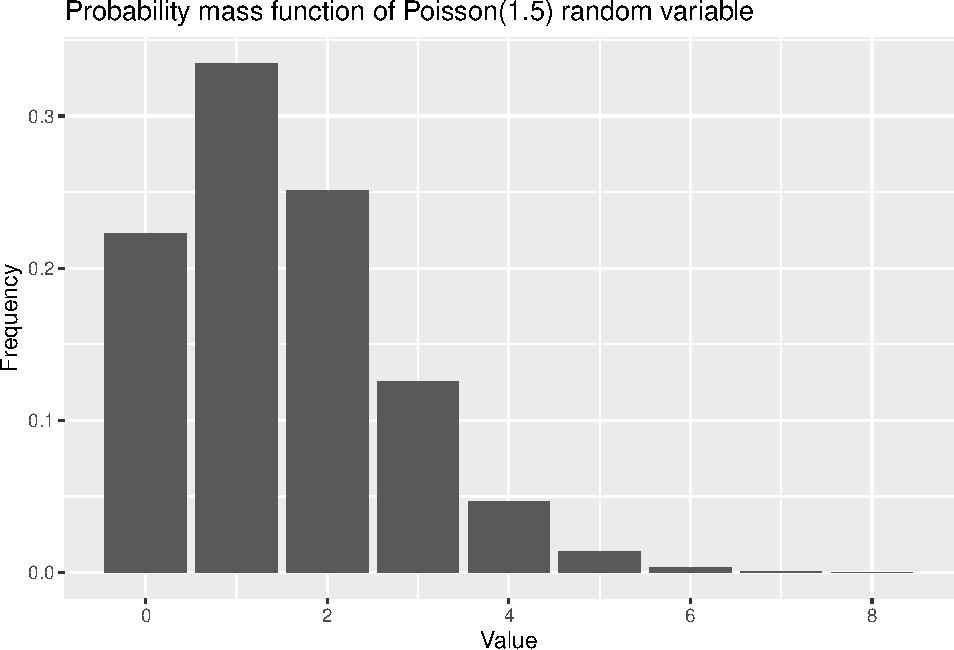
\includegraphics{textbook_files/figure-latex/unnamed-chunk-29-1.pdf}

Q: Which quadrant of the graph represents goalies that faced a higher than average number of shots, but had a below-average save percentage?

A: The second (upper left) quadrant.

Q: Which quadrant represents goalies that had a high save percentage and faced a high volume of shots?

A: The first (upper right) quadrant.

\hypertarget{correlation-plots}{%
\subsection{Correlation Plots}\label{correlation-plots}}

When analyzing sports data, there may be many circumstances where statisticians consider which of several variables are most highly correlated to an outcome variable of interest. In this case, it can be useful to use a correlation plot (also known as a correlation matrix or correlogram). Tidyverse and related packages provide many options for creating correlation plots.

Suppose a statistician has recently learned about some advanced hockey statistics and is interested in researching which stat has the highest correlation with goals scored. The statistician wants to compare team shots on goal, CORSI, and Fenwick to observe the association with goals scored for NHL teams.

\begin{example}
The following plot uses the same 2021-2022 data from Moneypuck.com; it gives the pairwise scatterplots and correlation values for each of the variables, as well as smoothed plots of each individual variable along the diagonals.
\end{example}

\begin{Shaded}
\begin{Highlighting}[]
\NormalTok{goal\_stats }\OtherTok{\textless{}{-}}\NormalTok{ nhl\_data\_all }\SpecialCharTok{\%\textgreater{}\%} \FunctionTok{select}\NormalTok{(shotsOnGoalFor, corsiPercentage, fenwickPercentage, goalsFor)}
\FunctionTok{ggpairs}\NormalTok{(goal\_stats, }\AttributeTok{title=}\StringTok{"Correlation plot of goals and relevant predictors, NHL 2021{-}22"}\NormalTok{)}
\end{Highlighting}
\end{Shaded}

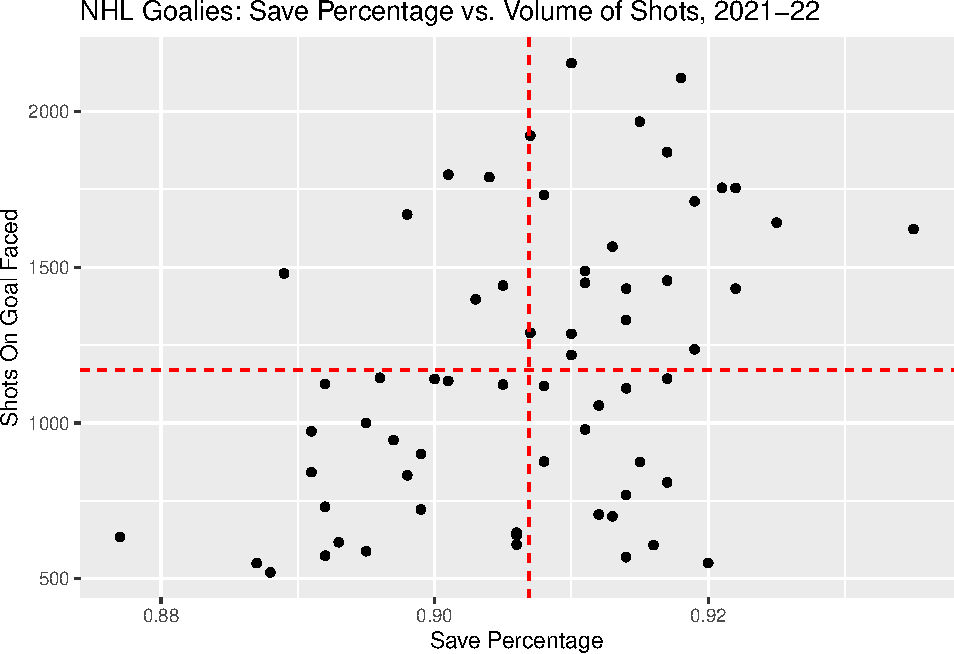
\includegraphics{textbook_files/figure-latex/unnamed-chunk-30-1.pdf}

Q: Which of the variables has the strongest correlation with goals scored?

A: CORSI percentage, r = .702.

In the article \href{https://theathletic.com/121980/2017/10/09/an-advanced-stat-primer-understanding-basic-hockey-metrics/}{``An advanced stat primer: Understanding basic hockey metrics''}, Charlie O'Connor states, ``Generally speaking, Corsi is more predictive of future goal differential than Fenwick\ldots{} however, Fenwick forms the basis for the most widely-used Expected Goals models.'' Let's use the same predictors in a correlation plot with Expected Goals percentage. Does Fenwick have the strongest correlation with xGoal percentage?

\begin{Shaded}
\begin{Highlighting}[]
\NormalTok{xGoal\_stats }\OtherTok{\textless{}{-}}\NormalTok{ nhl\_data\_all }\SpecialCharTok{\%\textgreater{}\%} 
  \FunctionTok{select}\NormalTok{(shotsOnGoalFor, corsiPercentage, fenwickPercentage, xGoalsPercentage)}
\FunctionTok{ggpairs}\NormalTok{(xGoal\_stats,}
        \AttributeTok{title=}\StringTok{"Correlation plot of expected goals and relevant predictors, NHL 2021{-}22"}\NormalTok{)}
\end{Highlighting}
\end{Shaded}

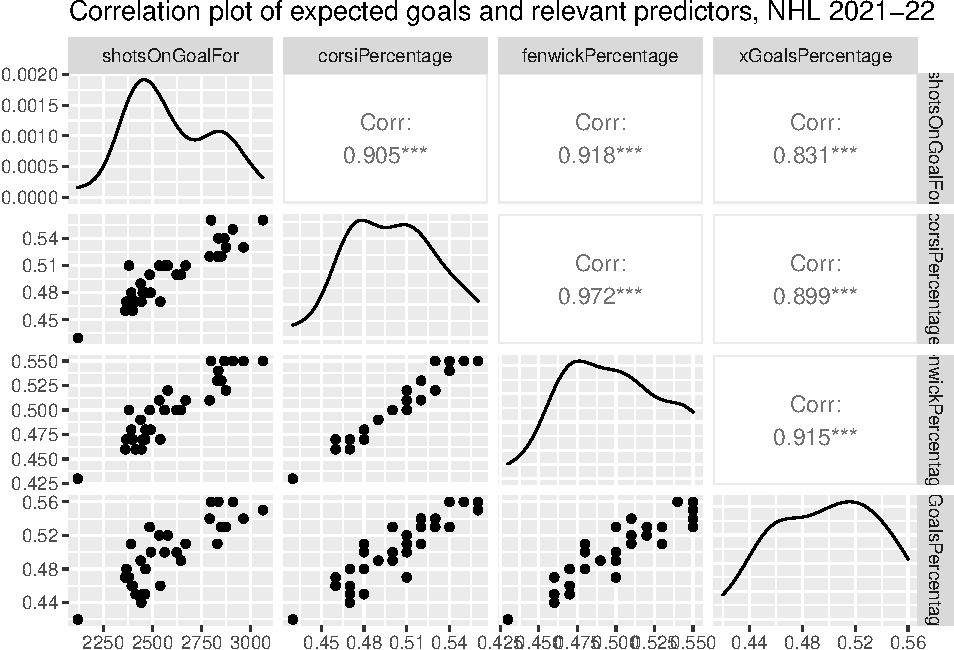
\includegraphics{textbook_files/figure-latex/hockey ggplot 6-1.pdf}

\newpage

\hypertarget{volleyball}{%
\section{Volleyball}\label{volleyball}}

Volleyball rules Youtube video: \url{https://www.youtube.com/watch?v=9g7nYQv-kPM}

\hypertarget{basic-volleyball-statistics}{%
\subsection{Basic Volleyball Statistics}\label{basic-volleyball-statistics}}

\begin{itemize}
\tightlist
\item
  A \textbf{Service Ace (SA)} occurs when a player's serve touches the ground on the other team's side without being touched by a player on that side.
\item
  A \textbf{Kill (K)} occurs when a player gets the ball over the net without it being returned by the opponent.
\item
  An \textbf{Assist (AST)} is a pass made directly before a player makes a kill.
\item
  \textbf{Hitting Percentage (PCT)} is the number of attempted kills (minus errors) divided by the total number of kill attempts. This helps determine how well a player or team is succeeding at their kill attempts.
\end{itemize}

\emph{Reference:}\\
www.rookieroad.com

For Volleyball EDA, we will be using CSU Women's Volleyball data from the last five seasons.

\begin{Shaded}
\begin{Highlighting}[]
\CommentTok{\# Load CSU Women\textquotesingle{}s Volleyball Data}
\NormalTok{csu\_vb }\OtherTok{\textless{}{-}} \FunctionTok{read\_csv}\NormalTok{(}\StringTok{"data/csu\_volleyball.csv"}\NormalTok{)}
\FunctionTok{colnames}\NormalTok{(csu\_vb)[}\DecValTok{3}\NormalTok{] }\OtherTok{\textless{}{-}} \StringTok{"W\_L"}
\NormalTok{csu\_vb }\SpecialCharTok{\%\textgreater{}\%} \FunctionTok{slice\_head}\NormalTok{(}\AttributeTok{n=}\DecValTok{10}\NormalTok{) }\SpecialCharTok{\%\textgreater{}\%} \FunctionTok{select}\NormalTok{(}\DecValTok{1}\SpecialCharTok{:}\DecValTok{13}\NormalTok{) }\SpecialCharTok{\%\textgreater{}\%} \FunctionTok{kt}\NormalTok{()}
\end{Highlighting}
\end{Shaded}

\begin{table}[H]
\centering
\begin{tabular}{l|c|c|c|c|c|c|c|c|l|c|c|c}
\hline
Date & Opponent & W\_L & SP & K & E & TA & PCT & AST & SA & SE & RE & DIG\\
\hline
8/25/17 & Duke & L & 5 & 66 & 28 & 179 & 0.212 & 64 & 5 & 13 & 6 & 84\\
\hline
8/26/17 & Central Florida & W & 4 & 56 & 18 & 126 & 0.302 & 52 & 7 & 10 & 7 & 49\\
\hline
8/29/17 & Northern Colorado & W & 3 & 39 & 8 & 77 & 0.403 & 38 & 5 & 12 & 4 & 29\\
\hline
9/1/17 & vs TCU & W & 5 & 62 & 20 & 149 & 0.282 & 59 & 6 & 10 & 7 & 65\\
\hline
9/1/17 & vs UNC Asheville & W & 3 & 41 & 7 & 80 & 0.425 & 39 & 8 & 8 & 5 & 28\\
\hline
9/2/17 & at Florida State & W & 3 & 48 & 12 & 95 & 0.379 & 45 & 6 & 4 & 1 & 42\\
\hline
9/8/17 & Ball State & W & 4 & 59 & 24 & 145 & 0.241 & 56 & 6 & 8 & 3 & 44\\
\hline
9/8/17 & Michigan & W & 3 & 48 & 8 & 101 & 0.396 & 46 & 3 & 6 & 4 & 37\\
\hline
9/10/17 & Idaho State & W & 3 & 46 & 11 & 92 & 0.380 & 46 & 4 & 3 & 4 & 48\\
\hline
9/15/17 & UAlbany & W & 3 & 41 & 7 & 73 & 0.466 & 36 & 5 & 5 & 1 & 30\\
\hline
\end{tabular}
\end{table}

Let's look at a scatter plot of hitting percentage and the number of digs. While no conclusions can be drawn from such a plot, it can give us some insight into relationships worthy of further analysis. Before creating the plot using the code below, think about what you might expect the outcome to be.

\hypertarget{scatter-plot}{%
\subsection{Scatter Plot}\label{scatter-plot}}

\begin{Shaded}
\begin{Highlighting}[]
\CommentTok{\# Digs, Hitting Percentage, Win/Lose}
\NormalTok{dig\_pct\_viz }\OtherTok{\textless{}{-}} \FunctionTok{ggplot}\NormalTok{(}\AttributeTok{data =}\NormalTok{ csu\_vb, }\FunctionTok{aes}\NormalTok{(}\AttributeTok{x =}\NormalTok{ DIG, }\AttributeTok{y =}\NormalTok{ PCT, }\AttributeTok{color =}\NormalTok{ W\_L)) }\SpecialCharTok{+}
  \FunctionTok{geom\_point}\NormalTok{()}
\NormalTok{dig\_pct\_viz}
\end{Highlighting}
\end{Shaded}

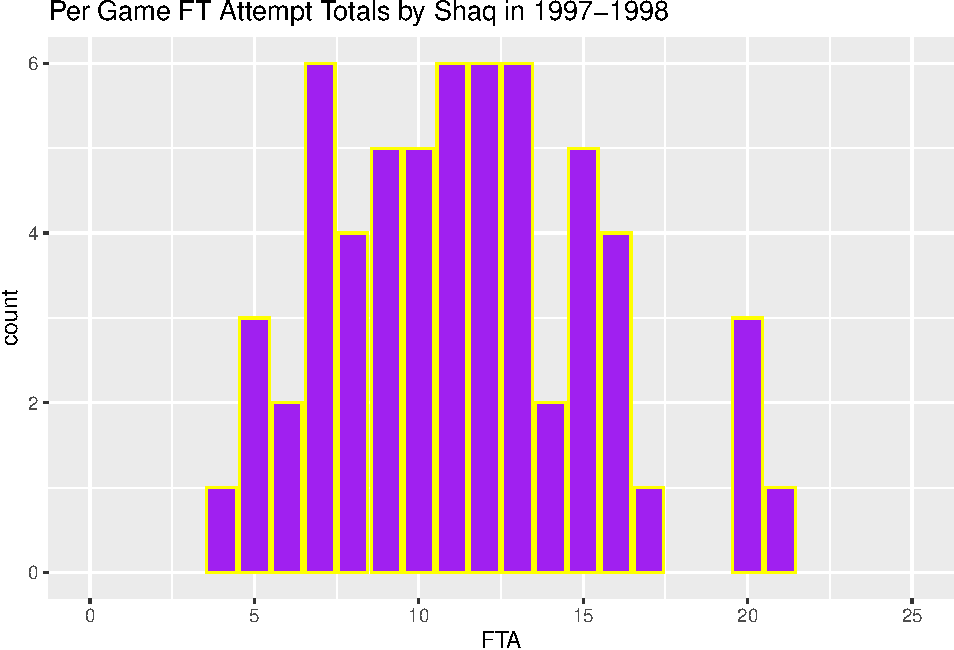
\includegraphics{textbook_files/figure-latex/unnamed-chunk-32-1.pdf}

Let's change the axis titles, legend title, and add a main title.

\begin{Shaded}
\begin{Highlighting}[]
\NormalTok{dig\_pct\_viz }\SpecialCharTok{+}
  \FunctionTok{labs}\NormalTok{(}\AttributeTok{title =} \StringTok{"Wins and Losses by Number of Digs and Hitting Percentage"}\NormalTok{,}
       \AttributeTok{x =} \StringTok{"Number of Digs (DIG)"}\NormalTok{, }\AttributeTok{y =} \StringTok{"Hitting Percentage (PCT)"}\NormalTok{,}
       \AttributeTok{color =} \StringTok{"Win or Loss"}\NormalTok{)}
\end{Highlighting}
\end{Shaded}

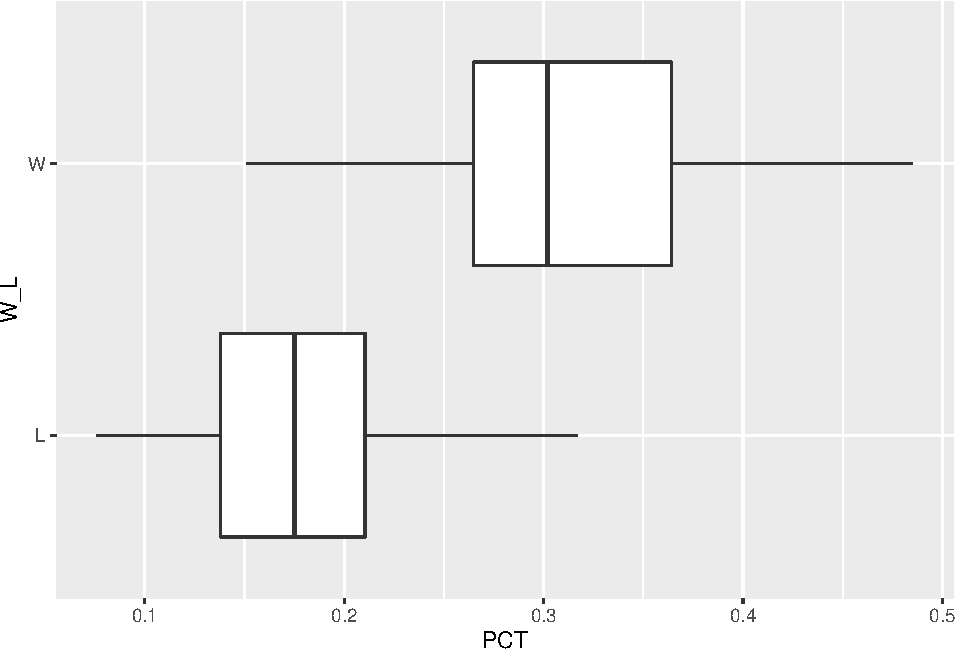
\includegraphics{textbook_files/figure-latex/unnamed-chunk-33-1.pdf}

What can we learn from this visual? Well, we can see that there is a weak linear relationship between the number of digs and hitting percentage. To an extent, hitting percentage decreases as the number of digs increases. Why is this the case? Maybe if a team has a really high hitting percentage, this means that the opposing team does not have as many opportunities to attack the other team offensively, reducing the number of opportunities for digs. It also seems that while wins and losses are somewhat evenly spread across the number of digs, there is a more clear cutoff for hitting percentage. It seems that the majority of wins are associated with a hitting percentage of at least 0.2, while the majority of losses are associated with a hitting percentage of less than 0.3.

\hypertarget{box-plot}{%
\subsection{Box Plot}\label{box-plot}}

Now let's take a closer look at the distribution of hitting percentage and digs for wins and losses. To do this, we will create box plots for each statistic.

\begin{Shaded}
\begin{Highlighting}[]
\NormalTok{pct\_viz }\OtherTok{\textless{}{-}} \FunctionTok{ggplot}\NormalTok{(}\AttributeTok{data =}\NormalTok{ csu\_vb, }\FunctionTok{aes}\NormalTok{(}\AttributeTok{x =}\NormalTok{ PCT, }\AttributeTok{y =}\NormalTok{ W\_L)) }\SpecialCharTok{+}
  \FunctionTok{geom\_boxplot}\NormalTok{()}
\NormalTok{pct\_viz}
\end{Highlighting}
\end{Shaded}

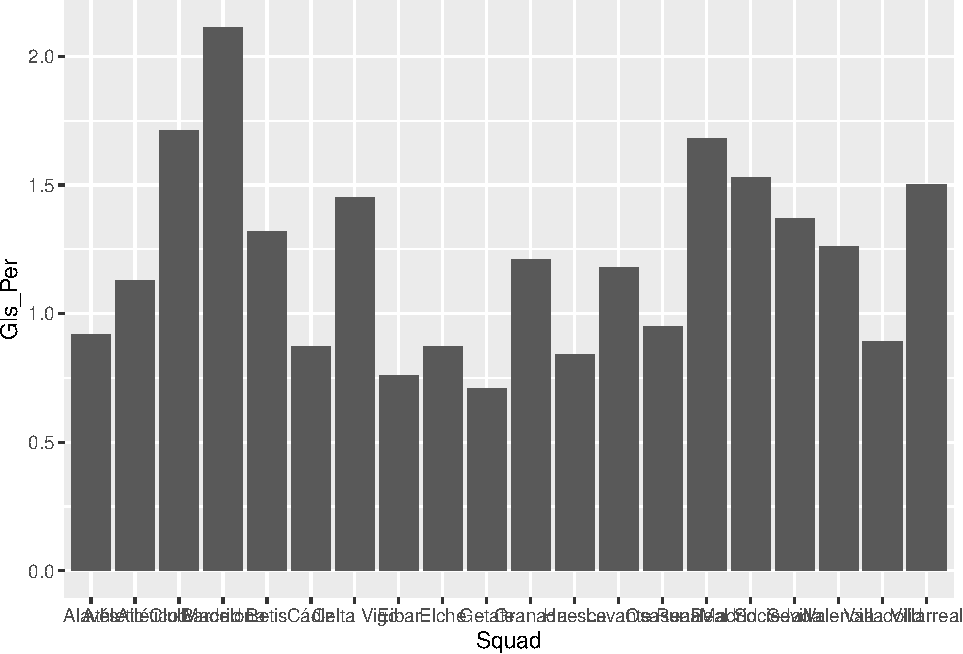
\includegraphics{textbook_files/figure-latex/unnamed-chunk-34-1.pdf}

\begin{Shaded}
\begin{Highlighting}[]
\NormalTok{dig\_viz }\OtherTok{\textless{}{-}} \FunctionTok{ggplot}\NormalTok{(}\AttributeTok{data =}\NormalTok{ csu\_vb, }\FunctionTok{aes}\NormalTok{(}\AttributeTok{x =}\NormalTok{ DIG, }\AttributeTok{y =}\NormalTok{ W\_L)) }\SpecialCharTok{+}
  \FunctionTok{geom\_boxplot}\NormalTok{()}
\NormalTok{dig\_viz}
\end{Highlighting}
\end{Shaded}

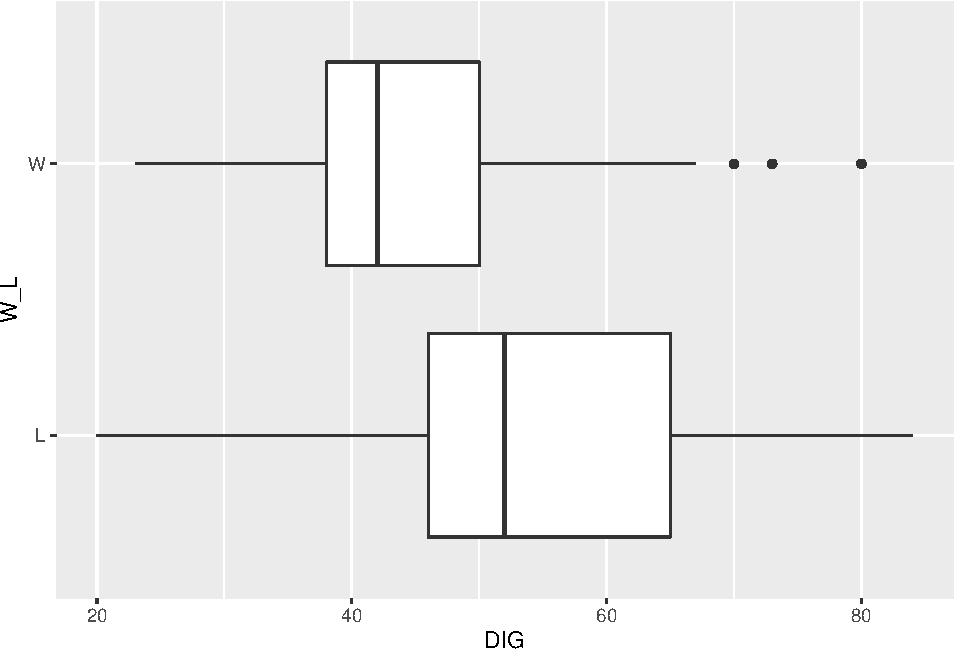
\includegraphics{textbook_files/figure-latex/unnamed-chunk-34-2.pdf}

Let's modify these plots to make them more complete and visually appealing.

\begin{Shaded}
\begin{Highlighting}[]
\NormalTok{pct\_viz }\SpecialCharTok{+}
  \FunctionTok{labs}\NormalTok{(}\AttributeTok{title =} \StringTok{"Hitting Percentage for Wins and Losses"}\NormalTok{,}
       \AttributeTok{x =} \StringTok{"Hitting Percentage (PCT)"}\NormalTok{,}
       \AttributeTok{y =} \StringTok{"Win or Loss"}\NormalTok{) }\SpecialCharTok{+}
  \FunctionTok{geom\_boxplot}\NormalTok{(}\AttributeTok{fill =} \StringTok{"slateblue"}\NormalTok{, }\AttributeTok{alpha =} \FloatTok{0.2}\NormalTok{)}
\end{Highlighting}
\end{Shaded}

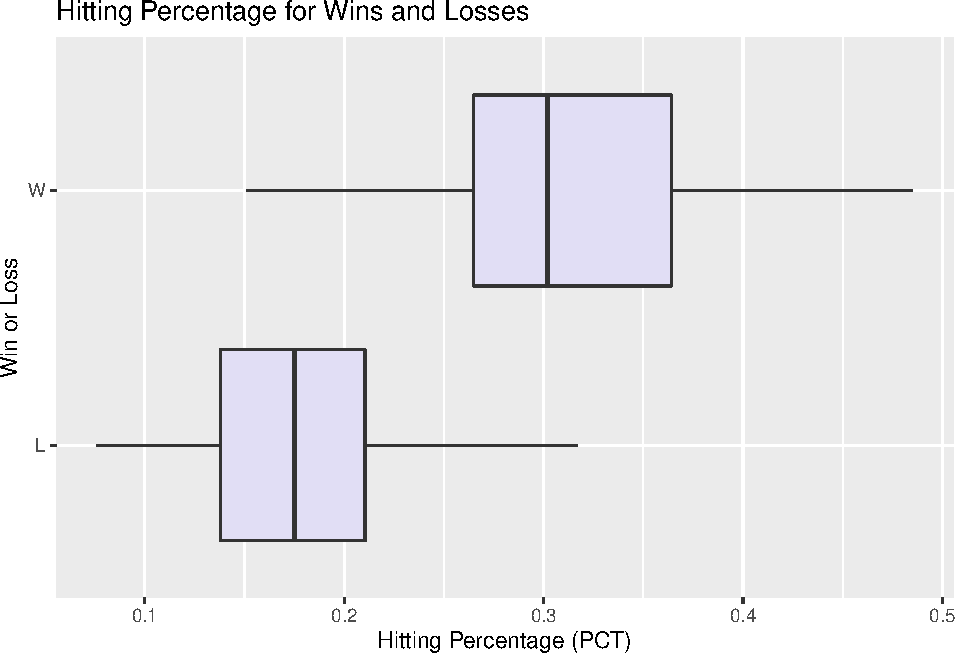
\includegraphics{textbook_files/figure-latex/unnamed-chunk-35-1.pdf}

\begin{Shaded}
\begin{Highlighting}[]
\NormalTok{dig\_viz }\SpecialCharTok{+}
  \FunctionTok{labs}\NormalTok{(}\AttributeTok{title =} \StringTok{"Number of Digs for Wins and Losses"}\NormalTok{,}
       \AttributeTok{x =} \StringTok{"Number of Digs (DIG)"}\NormalTok{,}
       \AttributeTok{y =} \StringTok{"Win or Loss"}\NormalTok{) }\SpecialCharTok{+}
  \FunctionTok{geom\_boxplot}\NormalTok{(}\AttributeTok{fill =} \StringTok{"slateblue"}\NormalTok{, }\AttributeTok{alpha =} \FloatTok{0.2}\NormalTok{)}
\end{Highlighting}
\end{Shaded}

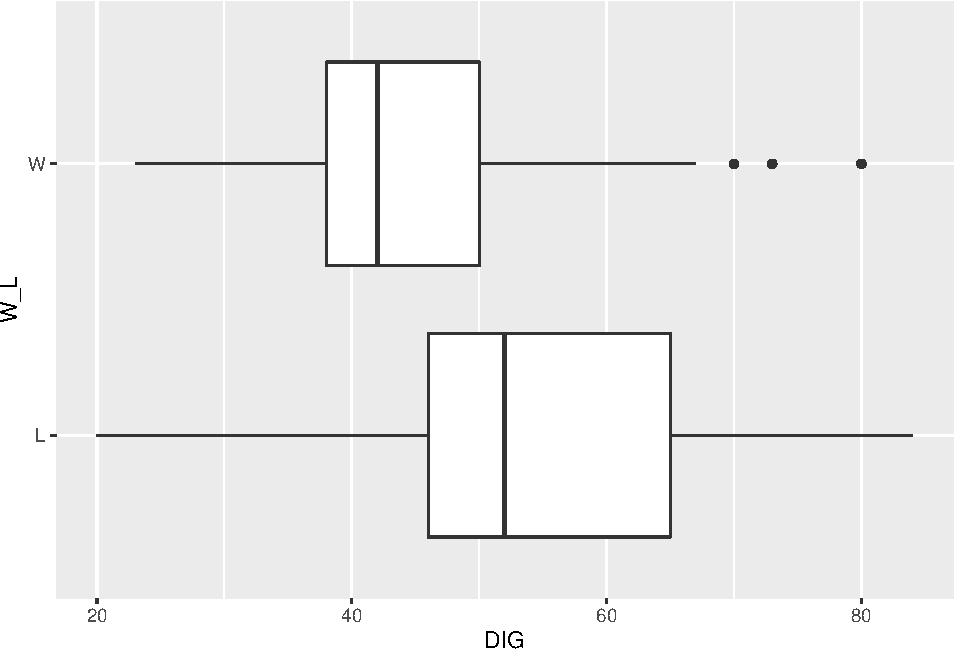
\includegraphics{textbook_files/figure-latex/unnamed-chunk-35-2.pdf}

Box plots allow us to isolate each statistic (number of kills and hitting percentage) so we can more clearly determine the center and spread of each between wins and losses.

\newpage

\hypertarget{soccer}{%
\section{Soccer}\label{soccer}}

Rules of Soccer YouTube video: \url{https://www.youtube.com/watch?v=dFLaabgXhpc}

\hypertarget{basic-soccer-statistics}{%
\subsection{Basic Soccer Statistics}\label{basic-soccer-statistics}}

\begin{itemize}
\item
  \textbf{Shots (SH)} represent all shots taken by a team throughout the game. This is simply an attempt by a player to shoot the ball toward the net, even if they miss or the shot is saved (Rookie Road).
\item
  \textbf{Shots on Goal (SOG)} represent all shots that would have gone into the goal if not saved by a defender or goalkeeper (Rookie Road).
\item
  \textbf{Assist (A)} occur when a player passes the ball to someone, and the next shot results in a goal.
\item
  \textbf{Possession} refers to the percentage of time a team had control of the ball during a game.
\end{itemize}

\hypertarget{advanced-soccer-statistics}{%
\subsection{Advanced Soccer Statistics}\label{advanced-soccer-statistics}}

\begin{itemize}
\tightlist
\item
  \textbf{Expected Goals (xG)} ``indicates how many goals a team could have expected to score based on the quantity and quality of chances that they created in a match'' (Tippett 2019, 4).
\end{itemize}

These definitions come from www.rookieroad.com and ``The Expected Goals Philosophy'' by James Tippett.

To learn more about expected goals, check out \href{https://www.youtube.com/watch?v=w7zPZsLGK18\&list=PL9Az6mi38hv__afKnHR1AKjpcDIw_0qqT}{this YouTube video}.

\hypertarget{bar-plot}{%
\subsection{Bar Plot}\label{bar-plot}}

Now that we have an understanding of some basic shooting statistics, let us go through some EDA examples. For this first example, we will need to install the ``worldfootballR'' package.

\begin{Shaded}
\begin{Highlighting}[]
\FunctionTok{library}\NormalTok{(worldfootballR)}
\end{Highlighting}
\end{Shaded}

Next we will look at some data specific to LaLiga, which is a soccer league in the men's top professional soccer division.

\begin{Shaded}
\begin{Highlighting}[]
\CommentTok{\# Get "Squad Standard Stats" Data}
\NormalTok{big5\_2021\_stats }\OtherTok{\textless{}{-}} \FunctionTok{fb\_big5\_advanced\_season\_stats}\NormalTok{(}\AttributeTok{season\_end\_year =} \DecValTok{2021}\NormalTok{, }\AttributeTok{stat\_type =} \StringTok{"standard"}\NormalTok{, }\AttributeTok{team\_or\_player =} \StringTok{"team"}\NormalTok{)}
\NormalTok{liga\_2021\_stats }\OtherTok{\textless{}{-}}\NormalTok{ big5\_2021\_stats[}\FunctionTok{which}\NormalTok{((big5\_2021\_stats}\SpecialCharTok{$}\NormalTok{Comp }\SpecialCharTok{==} \StringTok{"La Liga"}\NormalTok{)),]}

\CommentTok{\# look at the first ten entries and a selection of columns}
\NormalTok{liga\_2021\_stats }\SpecialCharTok{\%\textgreater{}\%} \FunctionTok{select}\NormalTok{(Squad,Team\_or\_Opponent,Poss,Gls,Ast,xG\_Expected,xA\_Expected) }\SpecialCharTok{\%\textgreater{}\%} \FunctionTok{slice\_head}\NormalTok{(}\AttributeTok{n=}\DecValTok{10}\NormalTok{) }\SpecialCharTok{\%\textgreater{}\%} \FunctionTok{kt}\NormalTok{()}
\end{Highlighting}
\end{Shaded}

\begin{Shaded}
\begin{Highlighting}[]
\CommentTok{\# Create visual for each team\textquotesingle{}s goals per game}
\NormalTok{team\_goals\_viz }\OtherTok{\textless{}{-}} 
  \FunctionTok{ggplot}\NormalTok{(}\AttributeTok{data =}\NormalTok{ liga\_2021\_stats[}\FunctionTok{which}\NormalTok{(liga\_2021\_stats}\SpecialCharTok{$}\NormalTok{Team\_or\_Opponent }\SpecialCharTok{==} \StringTok{"team"}\NormalTok{),], }
                         \FunctionTok{aes}\NormalTok{(}\AttributeTok{x =}\NormalTok{ Squad, }\AttributeTok{y =}\NormalTok{ Gls\_Per)) }\SpecialCharTok{+}
  \FunctionTok{geom\_bar}\NormalTok{(}\AttributeTok{stat =} \StringTok{"identity"}\NormalTok{)}
\NormalTok{team\_goals\_viz}
\end{Highlighting}
\end{Shaded}

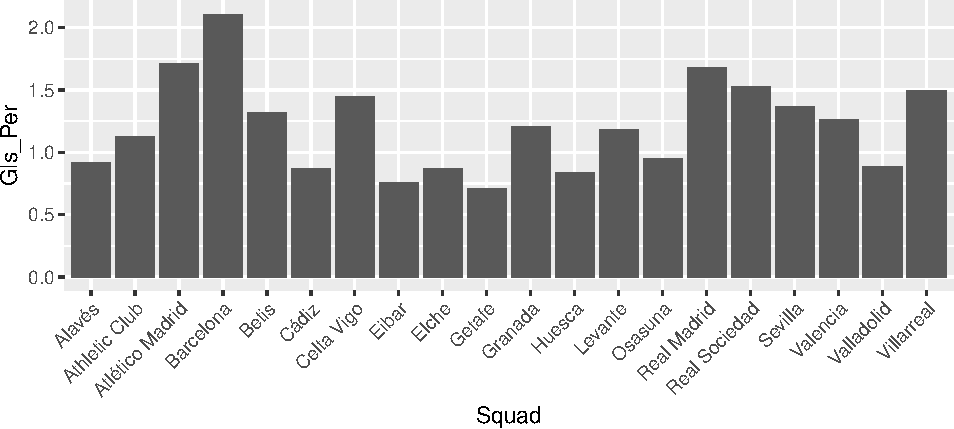
\includegraphics{textbook_files/figure-latex/unnamed-chunk-39-1.pdf}

This plot is a good starting point, but still looks pretty messy. Let's add a title, change the axis titles, and rotate the axis labels so they are not overlapping over one another.

\begin{Shaded}
\begin{Highlighting}[]
\NormalTok{team\_goals\_viz }\OtherTok{\textless{}{-}}\NormalTok{ team\_goals\_viz }\SpecialCharTok{+}
  \FunctionTok{xlab}\NormalTok{(}\StringTok{"Team"}\NormalTok{) }\SpecialCharTok{+}
  \FunctionTok{ylab}\NormalTok{(}\StringTok{"Goals Per Game"}\NormalTok{) }\SpecialCharTok{+}
  \FunctionTok{theme}\NormalTok{(}\AttributeTok{axis.text.x =} \FunctionTok{element\_text}\NormalTok{(}\AttributeTok{angle =} \DecValTok{45}\NormalTok{, }\AttributeTok{hjust =} \DecValTok{1}\NormalTok{)) }\SpecialCharTok{+}
  \FunctionTok{ggtitle}\NormalTok{(}\StringTok{"Goals Per Game by Team"}\NormalTok{)}
\NormalTok{team\_goals\_viz}
\end{Highlighting}
\end{Shaded}

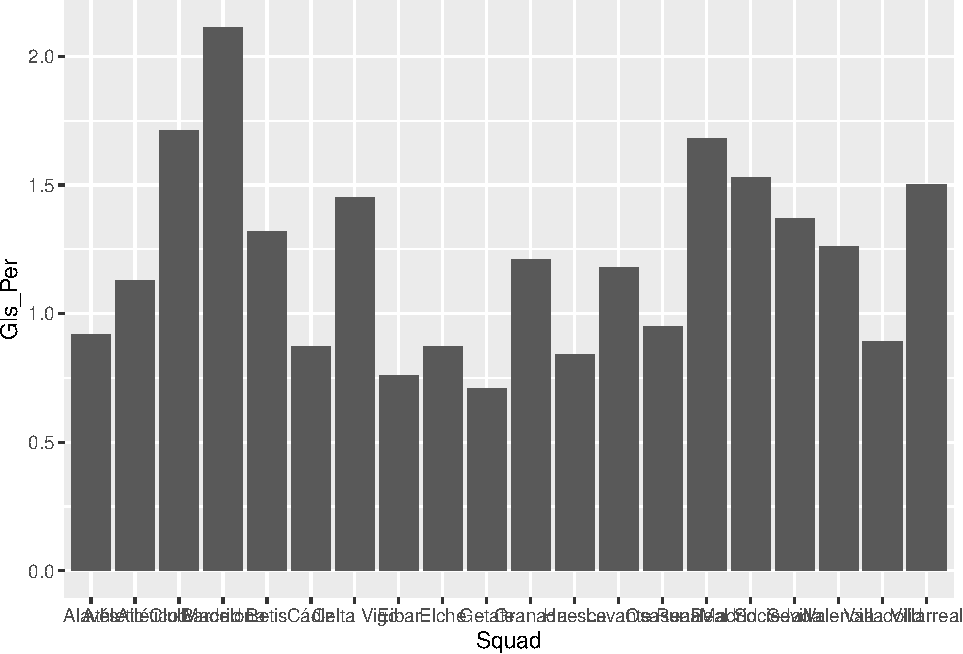
\includegraphics{textbook_files/figure-latex/unnamed-chunk-40-1.pdf}

This is already looking a lot better. Now, we will add the goals scored per game \emph{against} each team. Why is this of interest? Well, at first glance, Barcelona seems like a pretty impressive team, as they score more goals per game than any other team in the league. However, what if they also have more goals scored against them than any other team in the league? This could be important context, so we will include it in the graph below.

\begin{Shaded}
\begin{Highlighting}[]
\NormalTok{all\_goals\_viz }\OtherTok{\textless{}{-}} \FunctionTok{ggplot}\NormalTok{(}\AttributeTok{data =}\NormalTok{ liga\_2021\_stats, }\FunctionTok{aes}\NormalTok{(}\AttributeTok{x =}\NormalTok{ Squad, }\AttributeTok{y =}\NormalTok{ Gls\_Per)) }\SpecialCharTok{+}
  \FunctionTok{geom\_bar}\NormalTok{(}\AttributeTok{stat =} \StringTok{"identity"}\NormalTok{, }\FunctionTok{aes}\NormalTok{(}\AttributeTok{fill =}\NormalTok{ Team\_or\_Opponent), }\AttributeTok{position =} \StringTok{"stack"}\NormalTok{) }\SpecialCharTok{+}
  \FunctionTok{xlab}\NormalTok{(}\StringTok{"Team"}\NormalTok{) }\SpecialCharTok{+}
  \FunctionTok{ylab}\NormalTok{(}\StringTok{"Goals Per 90 Minutes"}\NormalTok{) }\SpecialCharTok{+}
  \FunctionTok{theme}\NormalTok{(}\AttributeTok{axis.text.x =} \FunctionTok{element\_text}\NormalTok{(}\AttributeTok{angle =} \DecValTok{45}\NormalTok{, }\AttributeTok{hjust =} \DecValTok{1}\NormalTok{)) }\SpecialCharTok{+}
  \FunctionTok{ggtitle}\NormalTok{(}\StringTok{"Goals Per Game by Team"}\NormalTok{)}
\NormalTok{all\_goals\_viz}
\end{Highlighting}
\end{Shaded}

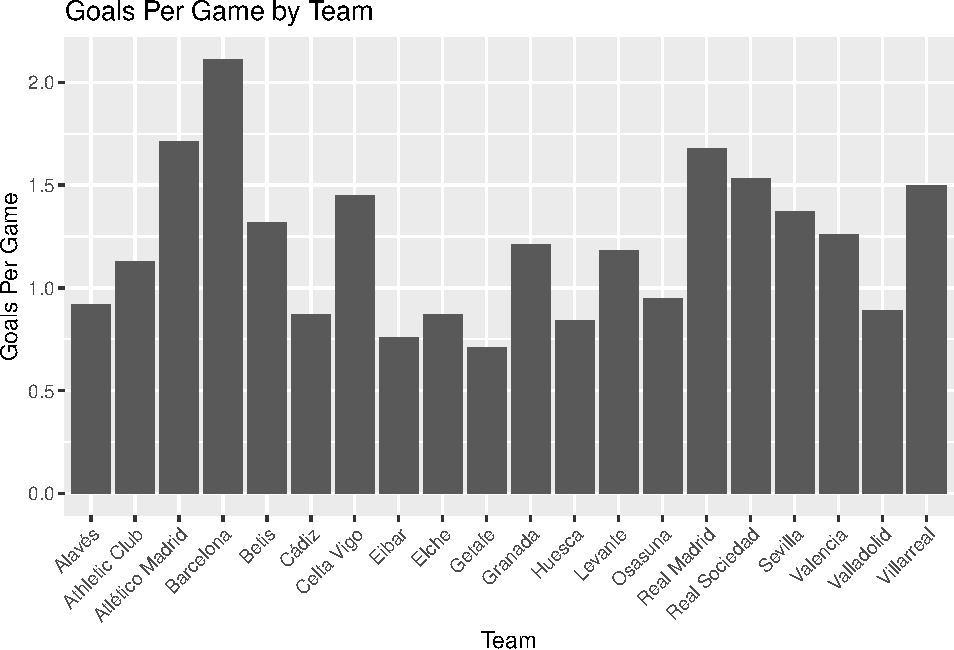
\includegraphics{textbook_files/figure-latex/unnamed-chunk-41-1.pdf}

This is looking pretty good, but let's clean it up just a bit by changing the legend title and labels.

\begin{Shaded}
\begin{Highlighting}[]
\NormalTok{all\_goals\_viz }\SpecialCharTok{+}
  \FunctionTok{scale\_fill\_discrete}\NormalTok{(}\AttributeTok{name =} \StringTok{"Team or Opponent"}\NormalTok{, }\AttributeTok{labels =} \FunctionTok{c}\NormalTok{(}\StringTok{"Opponent"}\NormalTok{,}\StringTok{"Team"}\NormalTok{))}
\end{Highlighting}
\end{Shaded}

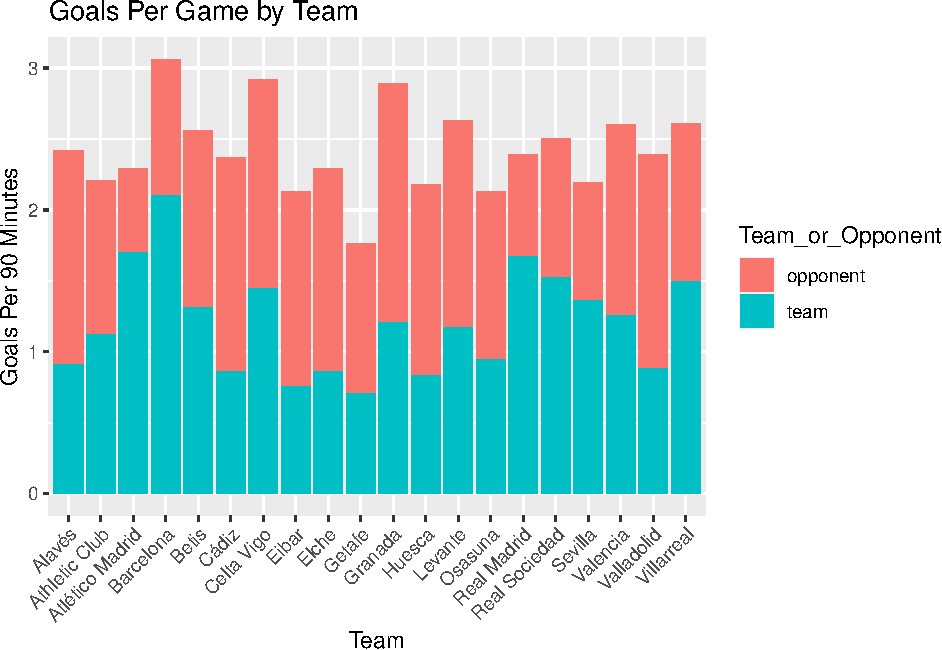
\includegraphics{textbook_files/figure-latex/unnamed-chunk-42-1.pdf}

What does this graph show us? Well, we are able to see the average number of goals scored for and against each team per game. It looks like Barcelona is scoring a lot more goals than they are letting be scored against them, while other teams like Valladolid tend to have a higher proportion of goals scored for the opposing team.

\hypertarget{scatter-plot-1}{%
\subsection{Scatter Plot}\label{scatter-plot-1}}

In addition to simply knowing the average actual number of goals scored for and against each team per game, we may be interested in how this compares to the expected number of goals scored per game, as well.

\begin{Shaded}
\begin{Highlighting}[]
\FunctionTok{library}\NormalTok{(ggExtra)}
\NormalTok{act\_exp\_viz }\OtherTok{\textless{}{-}} \FunctionTok{ggplot}\NormalTok{(}\AttributeTok{data =}\NormalTok{ liga\_2021\_stats, }\FunctionTok{aes}\NormalTok{(}\AttributeTok{x =}\NormalTok{ xG\_Per, }\AttributeTok{y =}\NormalTok{ Gls\_Per, }\AttributeTok{label =}\NormalTok{ Squad)) }\SpecialCharTok{+}
  \FunctionTok{geom\_point}\NormalTok{() }\SpecialCharTok{+}
  \FunctionTok{scale\_x\_continuous}\NormalTok{(}\AttributeTok{limits =} \FunctionTok{c}\NormalTok{(}\FloatTok{0.75}\NormalTok{,}\FloatTok{2.25}\NormalTok{)) }\SpecialCharTok{+}
  \FunctionTok{scale\_y\_continuous}\NormalTok{(}\AttributeTok{limits =} \FunctionTok{c}\NormalTok{(}\FloatTok{0.75}\NormalTok{,}\FloatTok{2.25}\NormalTok{)) }\SpecialCharTok{+}
  \FunctionTok{ggtitle}\NormalTok{(}\StringTok{"Expected vs. Actual Goals Per Game"}\NormalTok{) }\SpecialCharTok{+}
  \FunctionTok{xlab}\NormalTok{(}\StringTok{"Expected Goals Per Game"}\NormalTok{) }\SpecialCharTok{+}
  \FunctionTok{ylab}\NormalTok{(}\StringTok{"Actual Goals Per Game"}\NormalTok{) }\SpecialCharTok{+}
  \FunctionTok{geom\_smooth}\NormalTok{(}\AttributeTok{method =} \StringTok{"lm"}\NormalTok{, }\AttributeTok{se =} \ConstantTok{FALSE}\NormalTok{) }\SpecialCharTok{+}
  \FunctionTok{theme}\NormalTok{(}\AttributeTok{aspect.ratio =} \DecValTok{2}\SpecialCharTok{/}\DecValTok{2}\NormalTok{)}
\FunctionTok{ggMarginal}\NormalTok{(act\_exp\_viz, }\AttributeTok{type =} \StringTok{"density"}\NormalTok{)}
\end{Highlighting}
\end{Shaded}

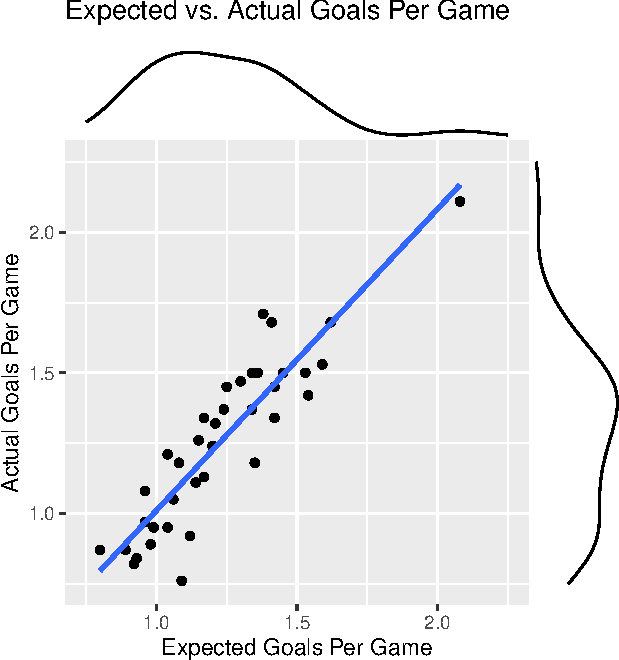
\includegraphics{textbook_files/figure-latex/unnamed-chunk-43-1.pdf}

As you can see, we fit a line to the data. At first glance, it seems to have a positive slope slightly greater than 1. What does this mean in the scenario of actual and expected goals per game?

\begin{example}
Use the \texttt{worldfootballR} package to collect team shooting data from the Women's 1st Tier League (Women's Super League) in England for 2020-2021. Plot goals vs.~shots, shots on target, and expected goals. Comment on the relationships.
\end{example}

\begin{Shaded}
\begin{Highlighting}[]
\NormalTok{wsl\_2021\_shooting }\OtherTok{\textless{}{-}} \FunctionTok{get\_season\_team\_stats}\NormalTok{(}
  \AttributeTok{country =} \StringTok{"ENG"}\NormalTok{, }\AttributeTok{gender =} \StringTok{"F"}\NormalTok{, }\AttributeTok{season\_end\_year =} \StringTok{"2021"}\NormalTok{, }\AttributeTok{tier =} \StringTok{"1st"}\NormalTok{, }\AttributeTok{stat\_type =} \StringTok{"shooting"}\NormalTok{)}
\NormalTok{wsl\_2021\_shooting }\OtherTok{\textless{}{-}}\NormalTok{wsl\_2021\_shooting }\SpecialCharTok{\%\textgreater{}\%} 
  \FunctionTok{select}\NormalTok{(Squad,Gls\_Standard,Sh\_Standard,SoT\_Standard,xG\_Expected) }\SpecialCharTok{\%\textgreater{}\%} 
  \FunctionTok{rename}\NormalTok{(}\AttributeTok{Goals=}\NormalTok{Gls\_Standard,}\AttributeTok{Shots=}\NormalTok{Sh\_Standard,}
         \StringTok{\textasciigrave{}}\AttributeTok{Shots on Target}\StringTok{\textasciigrave{}}\OtherTok{=}\NormalTok{SoT\_Standard,}\StringTok{\textasciigrave{}}\AttributeTok{Expected Goals}\StringTok{\textasciigrave{}} \OtherTok{=}\NormalTok{ xG\_Expected)}
\NormalTok{wsl\_2021\_shooting }\SpecialCharTok{\%\textgreater{}\%} \FunctionTok{kt}\NormalTok{()}
\end{Highlighting}
\end{Shaded}

\begin{table}[H]
\centering
\begin{tabular}{l|c|c|c|c}
\hline
Squad & Goals & Shots & Shots on Target & Expected Goals\\
\hline
Arsenal & 62 & 366 & 152 & 52.7\\
\hline
Aston Villa LFC & 14 & 159 & 45 & 15.3\\
\hline
Birmingham City & 14 & 116 & 35 & 10.8\\
\hline
Brighton & 20 & 207 & 68 & 20.8\\
\hline
Bristol City & 17 & 186 & 61 & 17.2\\
\hline
Chelsea & 67 & 425 & 150 & 57.4\\
\hline
Everton & 39 & 248 & 82 & 31.0\\
\hline
Manchester City & 62 & 420 & 143 & 55.5\\
\hline
Manchester Utd & 43 & 380 & 132 & 42.1\\
\hline
Reading & 24 & 281 & 93 & 28.5\\
\hline
Tottenham & 16 & 196 & 64 & 19.5\\
\hline
West Ham & 18 & 228 & 80 & 22.8\\
\hline
vs Arsenal & 14 & 169 & 51 & 15.3\\
\hline
vs Aston Villa LFC & 45 & 355 & 121 & 39.8\\
\hline
vs Birmingham City & 43 & 370 & 126 & 39.9\\
\hline
vs Brighton & 41 & 316 & 93 & 39.2\\
\hline
vs Bristol City & 68 & 426 & 165 & 51.7\\
\hline
vs Chelsea & 9 & 143 & 35 & 12.7\\
\hline
vs Everton & 29 & 243 & 86 & 30.4\\
\hline
vs Manchester City & 13 & 122 & 40 & 13.1\\
\hline
vs Manchester Utd & 17 & 202 & 67 & 20.2\\
\hline
vs Reading & 41 & 296 & 103 & 38.9\\
\hline
vs Tottenham & 39 & 276 & 102 & 35.2\\
\hline
vs West Ham & 37 & 294 & 116 & 37.1\\
\hline
\end{tabular}
\end{table}

\begin{Shaded}
\begin{Highlighting}[]
\NormalTok{wsl\_2021\_shooting }\OtherTok{\textless{}{-}}\NormalTok{ wsl\_2021\_shooting }\SpecialCharTok{\%\textgreater{}\%}
  \FunctionTok{slice\_head}\NormalTok{(}\AttributeTok{n=}\DecValTok{12}\NormalTok{)}
\NormalTok{wsl\_2021\_shooting }\SpecialCharTok{\%\textgreater{}\%} 
  \FunctionTok{select}\NormalTok{(Goals,Shots,}\StringTok{\textasciigrave{}}\AttributeTok{Shots on Target}\StringTok{\textasciigrave{}}\NormalTok{,}\StringTok{\textasciigrave{}}\AttributeTok{Expected Goals}\StringTok{\textasciigrave{}}\NormalTok{) }\SpecialCharTok{\%\textgreater{}\%} 
  \FunctionTok{ggpairs}\NormalTok{()}
\end{Highlighting}
\end{Shaded}

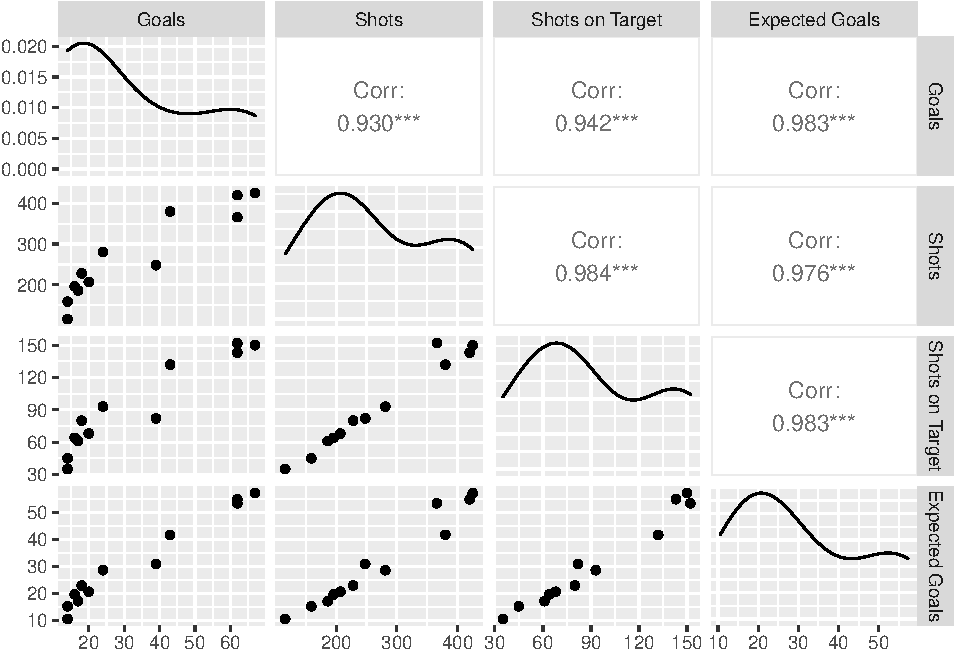
\includegraphics{textbook_files/figure-latex/unnamed-chunk-45-1.pdf}

\hypertarget{probability}{%
\chapter{Probability}\label{probability}}

\hypertarget{chapter-preview}{%
\section*{Chapter Preview}\label{chapter-preview}}
\addcontentsline{toc}{section}{Chapter Preview}

Probability is the study of randomness. In this chapter, we will define probability, learn rules of probability, and apply these rules to sports data.

\hypertarget{definitions-1}{%
\section{Definitions}\label{definitions-1}}

\begin{definition}
An \textbf{\emph{experiment}} is any activity or process whose outcome is subject to uncertainty.
\end{definition}

\begin{definition}
The \textbf{\emph{sample space}} of an experiment, denoted by \(\Omega\) or \(\mathcal{S}\), is the set of all possible outcomes of that experiment.
\end{definition}

\begin{definition}
An \textbf{\emph{event}} is any collection (subset) of outcomes contained in the sample space, \(\Omega\).
\end{definition}

\begin{example}
Give an example of a discrete random variable in a sports context.
\end{example}

\hfill\break
\hfill\break
\hfill\break
\hfill\break
\hfill\break

\begin{example}
Give an example of a continuous random variable in a sports context.
\end{example}

~\\
\strut \\
\strut \\
\strut \\

\newpage

\hypertarget{set-theory}{%
\section{Set Theory}\label{set-theory}}

For the following examples, suppose that we are interested in the batting outcomes of a plate appearance in softball.

Let \(A\) be the event that the batter gets walked, let \(B\) be the event that the batter gets a hit, let \(C\) be the event that the batter strikes out, and let \(D\) be the event that the batter makes it to first base at the end of their at bat.

We will define a handful of set operations to help us when we begin calculating the probability of different events occurring.

\begin{definition}
The \textbf{\emph{compliment}} of an event \(A\), denoted by \(A^c\) or \(A'\), is the set of all outcomes in \(\Omega\) that are not contained in \(A\).
\end{definition}

\begin{example}
Draw a Venn diagram illustrating \(A^c\) and describe the event.
\end{example}

\hfill\break
\hfill\break
\hfill\break
\hfill\break
\hfill\break

\begin{definition}
The \textbf{\emph{union}} of two events \(A\) and \(B\), denoted by \(A \cup B\) and read ``\(A\) or \(B\)'', is the event consisting of all outcomes that are either in \(A\) or \(B\) or in both.
\end{definition}

\begin{example}
Draw a Venn diagram illustrating \(A \cup D\) and describe the event.
\end{example}

\hfill\break
\hfill\break
\hfill\break
\hfill\break
\hfill\break

\begin{definition}
The \textbf{\emph{intersection}} of two events \(A\) and \(B\), denoted by \(A \cap B\) and read ``\(A\) and \(B\)'', is the event consisting of all outcomes that are in both \(A\) and \(B\).
\end{definition}

\begin{example}
Draw a Venn diagram illustrating \(A \cap D\) and describe the event.
\end{example}

\hfill\break
\hfill\break
\hfill\break
\hfill\break
\hfill\break

\begin{definition}
The \textbf{\emph{difference}} of two events \(A\) and \(B\), denoted by \(A \mathbin{/} B\) and read ``difference of \(A\) and \(B\)'', is
the event consisting of all outcomes that are in \(A\) but not in \(B\).
\end{definition}

\begin{example}
Draw a Venn diagram illustrating \(D \mathbin{/} A\) and describe the event.
\end{example}

\hfill\break
\hfill\break
\hfill\break
\hfill\break
\hfill\break

\begin{definition}
Two events \(A\) and \(B\) are said to be \textbf{\emph{disjoint}} (or \textbf{\emph{mutually exclusive}}) if \(A \cap B = \emptyset\)
\end{definition}

\begin{example}
Are the events \(A\) and \(B\) disjoint? How about \(A\) and \(D\)?
\end{example}

\hfill\break
\hfill\break
\hfill\break
\hfill\break
\hfill\break

\newpage

\hypertarget{axioms-properties-and-laws}{%
\section{Axioms, Properties, and Laws}\label{axioms-properties-and-laws}}

There are some basic assumptions of ``axioms'' which are the foundation of the theory of probability. Andrey Kolmogorov first described these axioms in 1933.

\hypertarget{axioms-of-probability}{%
\subsection{Axioms of Probability}\label{axioms-of-probability}}

\begin{enumerate}
\def\labelenumi{\arabic{enumi}.}
\tightlist
\item
  \(P(A) \geq 0\), for any event \(A\)\\
\item
  \(P(\Omega) = 1\)\\
\item
  If \(A_1, A_2, A_3, \ldots\) is a collection of disjoint events, then:\\
  \(P(\cup_{i=1}^{\infty} A_i) = P(A_1 \cup A_2 \cup \ldots ) = \sum_{i=1}^{\infty} P(A_i)\)
\end{enumerate}

Note that all probabilities are between 0 and 1, that is, for any event \(A\), \(0 \leq P(A) \leq 1\).

We can convert to percentages by multiplying probabilities by 100, however, this is a set that is only done after all calculations have been completed.

\hypertarget{properties-of-probability}{%
\subsection{Properties of Probability}\label{properties-of-probability}}

\begin{itemize}
\item
  \(P(\emptyset) = 0\)\\
\item
  \(P(A^c) = 1 - P(A)\)
\item
  \(P(A \cup B) = P(A) + P(B) - P(A \cap B)\)
\item
  \(P(A \cup B \cup C) = \\ P(A) + P(B) + P(C) - P(A \cap B) - P(A \cap C) - P(B \cap C) + P(A \cap B \cap C)\)
\item
  \(P([A \cup B]^c) = P(A^c \cap B^c)\)
\item
  \(P([A \cap B]^c) = P(A^c \cup B^c)\)
\end{itemize}

\newpage

\begin{example}
In 2001, Barry Bonds broke the single season home run record with 73 home runs. In this season, he had 664 plate appearances (476 at-bats), 156 hits, 177 walks, 9 hit by pitches, and 2 sacrifice flies. Use this information to answer the following questions.
\end{example}

\begin{enumerate}
\def\labelenumi{(\alph{enumi})}
\item
  Plate appearances that result in a walk, hit by pitch, or sacrifice fly are not counted towards a player's at-bats. Confirm that Bonds had 476 official at-bats.\\
  \strut \\
  \strut \\
  \strut \\
  \vfill
\item
  Suppose an at-bat is chosen at random. What is the probability that Bonds got a hit? (This is his batting average.)\\
  \strut \\
  \strut \\
  \strut \\
  \vfill
\end{enumerate}

\emph{For the following examples, assume that one of Bonds' plate appearances is chosen at random.}\\

\begin{enumerate}
\def\labelenumi{(\alph{enumi})}
\setcounter{enumi}{2}
\item
  What is the probability that Bonds reached base via a hit, walk, or hit by pitch? (This is his on-base average/percentage.)\\
  \strut \\
  \strut \\
  \strut \\
  \vfill
\item
  What is the probability that Bonds did not reach base?\\
  \strut \\
  \strut \\
  \strut \\
  \vfill
\item
  Calculate \(P\left(HBP \cup Walk\right)\)\\
  \strut \\
  \strut \\
  \strut \\
  \vfill
\item
  Calculate \(P\left(HBP^c \cap Walk^c\right)\)\\
  \strut \\
  \strut \\
  \strut \\
  \vfill
\end{enumerate}

\newpage

\hypertarget{laws-of-probability}{%
\subsection{Laws of Probability}\label{laws-of-probability}}

\begin{definition}
Let \(A\) and \(B\) be two events such that \(P(B)>0\). Then the \textbf{\emph{conditional probability}} of \(A\) given \(B\), written \(P(A|B)\), is given by:
\(P(A|B) = \frac{P(A \cap B)}{P(B)}\)
\end{definition}

\begin{example}
In 1998, Sammy Sosa hit 66 home runs in 722 plate appearances, the third highest single season homework total ever. During June 1998, Sosa 20 home runs in 121 plate appearances. Suppose a randomly selected plate appearance is selected. Calculate the following probabilities.
\end{example}

\begin{enumerate}
\def\labelenumi{(\alph{enumi})}
\item
  \(P(HR)\)\\
  \strut \\
  \strut \\
  \strut \\
  \vfill
\item
  \(P(HR \cap June)\)\\
  \strut \\
  \strut \\
  \strut \\
  \vfill
\item
  \(P(June)\)\\
  \strut \\
  \strut \\
  \strut \\
  \vfill
\item
  \(P(HR|June)\)\\
  \strut \\
  \strut \\
  \strut \\
  \vfill
\item
  \(P(June|HR)\)\\
  \strut \\
  \strut \\
  \strut \\
  \vfill
\item
  \(P(HR|June^c)\)\\
  \strut \\
  \strut \\
  \strut \\
  \vfill
\end{enumerate}

\begin{theorem}[Multiplication Rule]
For any two events \(A\) and \(B\), \(P(A \cap B) = P(B|A) \cdot P(A)\).
\end{theorem}

\begin{example}
Calculate the probability that a randomly selected plate appearance from Sosa's 1998 season is a home run in June.
\end{example}

\hfill\break
\hfill\break
\hfill\break
\vfill

\newpage

\begin{definition}
Events \(A_1, A_2, \ldots, A_n\) are said to form a \textbf{\emph{partition}} of a sample space \(\Omega\) if both:\\
(i) \(A_i \cap A_j = \emptyset\) (\(i \neq j\))\\
(ii) \(\cup_{i=1}^n A_i = \Omega\)\\

\end{definition}

\begin{theorem}[Law of Total Probability]
Suppose events \(A_1, A_2, \ldots, A_n\) form a partition of \(\Omega\), then:
\(P(B) = P(B|A_1)P(A_1) + P(B|A_2)P(A_2) + \ldots P(B|A_n)P(A_n)\)
\end{theorem}

\begin{example}
What is one possible way to partition Sosa's plate appearances in 1998?
\end{example}

\hfill\break
\hfill\break
\hfill\break

\begin{theorem}[Bayes Theorem: simple version]
Suppose events \(B\) and \(C\) form a partition of \(\Omega\), then:
\(P(B|A) = \frac{P(B \cap A)}{P(A)} = \frac{P(A|B)P(B)}{P(A|B)P(B)+P(A|C)P(C)}\)
\end{theorem}

\begin{theorem}[Bayes Theorem]
Suppose events \(B_1, B_2, \ldots, B_n\) form a partition of \(\Omega\), then:
\(P(B_k|A) = \frac{P(B_k \cap A)}{P(A)} = \frac{P(A|B_k)P(B_k)}{P(A|B_1)P(B_1)+P(A|B_2)P(B_2) + \ldots + P(A|B_n)P(B_n)}\)
\end{theorem}

\begin{example}
Given that Sosa hit a home run in 1998, what is the probability that he hit it in June?
\end{example}

\hfill\break
\hfill\break
\hfill\break

\begin{example}
Over the course of a season, a hockey player scored a goal 30\% of the time during a home game, and 18\%. Assume all games are either home or away. Use this information to answer the following questions.
\end{example}

\begin{enumerate}
\def\labelenumi{(\alph{enumi})}
\item
  What is the probability the player scored a goal in any game if there were an equal number of home and away games?\\
  \strut \\
  \strut \\
  \strut \\
\item
  What is the probability the player scored a goal in any game if there were twice as many home games as away games?\\
  \strut \\
  \strut \\
  \strut \\
\item
  What is the probability the player scored a goal in any game if the ratio of home games to away games is 2:3?\\
  \strut \\
  \strut \\
  \strut \\
\end{enumerate}

\newpage

\hypertarget{combinatorics}{%
\section{Combinatorics}\label{combinatorics}}

Combinatorics is the mathematical study of counting, particularly with respect to permutations and combinations.

\begin{definition}
The \textbf{\emph{factorial function (\(n!\))}} is defined for all positive integers by: \(n! = n \cdot (n-1) \cdot \ldots 2 \cdot 1\)
\end{definition}

Note that \(0! \equiv 1\) and \(1! \equiv 1\).

\begin{example}
A baseball/softball batting lineup has nine ordered players. Suppose the manager has selected the nine players to bat. How many different batting orders are there possible?
\end{example}

\hfill\break
\hfill\break
\hfill\break

\begin{definition}
An ordered subset is called a \textbf{\emph{permutation}}. The number of permutations of size \(k\) that can be formed from the \(n\) elements in a set is given by: \(P_{n,k} = \frac{n!}{(n-k)!}\)
\end{definition}

\begin{example}
In MLB, each team has a 26-person roster, of which about 13 are hitters. Assuming one of the batters is the designated hitter, how many different batting lineups of 9 players can a manager create?
\end{example}

\hfill\break
\hfill\break
\hfill\break

\begin{definition}
An unordered subset is called a \textbf{\emph{combination}}. The number of combinations of size \(k\) that can be formed from the \(n\) elements in a set is given by: \(C_{n,k} = {n \choose k} = \frac{n!}{k! \cdot (n-k)!}\)
\end{definition}

\begin{example}
Suppose a manager has 13 hitters to choose from to fill out a starting lineup of 9 players. Ignoring positions, how many different ways can the manager pick a 9-person lineup from 13 possible hitters?
\end{example}

\begin{theorem}[Product Rule for Ordered Pairs]
If the first element of an ordered pair can be selected in \(n_1\) ways and for each of the these \(n_1\) ways the second element of the pair can be selected in \(n_2\) ways, then the number of pairs is \(n_1 \cdot n_2\).
\end{theorem}

\hfill\break
\hfill\break
\hfill\break
\hfill\break

\begin{theorem}[Generalized Product Rule]
Suppose a set consists of \(k\) elements (k-tuples) and that there are \(n_1\) possible choices for the first element, \(n_2\) possible choices for the second element, \ldots{} , and \(n_k\) possible choices for the \(k^\text{th}\) element, then there are \(n_1 \cdot n_2 \cdot \ldots \cdot n_k\) possible k-tuples.
\end{theorem}

\begin{example}
A baseball manager selects nine hitters and one pitcher for a starting lineup. Suppose they can choose from 13 hitters and 13 hitters. How many different possible lineups can the manager choose from?
\end{example}

\hfill\break
\hfill\break
\hfill\break

\begin{example}
In softball, rules sometimes allow for a ``designated player''. This player hits for any position player or pitcher but isn't required to play defense. There is some flexibility to allow the designated player to temporarily play a position during the game however. For more on the designated player rule in softball, visit: \url{https://cdn2.sportngin.com/attachments/document/c780-2407390/DPFlexRuleExplained.pdf}

In 2022, the CSU softball team had 24 players. Three of these players were only pitchers and two of these players were both pitchers and fielders. How many different lineups of 10 (8 non-pitching position players, 1 pitcher, 1 designated player) are possible for CSU?
\end{example}

\hfill\break
\hfill\break
\hfill\break
\hfill\break

\newpage

\hypertarget{odds-and-gambling}{%
\section{Odds and Gambling}\label{odds-and-gambling}}

\hypertarget{sports-betting-in-usa}{%
\subsection{Sports Betting in USA}\label{sports-betting-in-usa}}

In 2018, the United States Supreme Court overturned a 1992 federal law that banned commercial sports betting in most states. For more about this ruling, see this New York Times article: \url{https://www.nytimes.com/2018/05/14/us/politics/supreme-court-sports-betting-new-jersey.html}

In Colorado, you must be at least 21 years old to gamble including betting on sports games.

\hypertarget{gambling-addiction}{%
\subsection{Gambling Addiction}\label{gambling-addiction}}

Gambling addiction, compulsive gambling, or gambling disorder is a serious impulse-control disorder. Here is a link to the Mayo Clinic's discussion of compulsive gambling: \url{https://www.mayoclinic.org/diseases-conditions/compulsive-gambling/symptoms-causes/syc-20355178}

Gambling is \textbf{\emph{not}} encouraged and can lead to numerous problems. If you choose to gamble on sports, don't bet beyond your means and seek help if you worry that you may be suffering from gambling addiction.

\hypertarget{odds-definition}{%
\subsection{Odds Definition}\label{odds-definition}}

In this chapter so far, we have quantified uncertainty using probabilities (numbers between 0 and 1) and percentages (numbers between 0 and 100). We can also quantify uncertainty using \textbf{odds}.

\begin{definition}
The \textbf{\emph{odds}} (in favor) of an outcome \(A\) is the probability of \(A\) divided by the probability of \(A^C\).

\[Odds = \frac{p}{1-p}\]
\end{definition}

\textbf{Note:} We may also be given the \textbf{odds against} a particular outcome. In this case, we have \(Odds Against = \frac{1-p}{p}\).\\

\textbf{Some Common Odds:}

\begin{table}[H]
\centering
\begin{tabular}{c|c|c|c|c|c}
\hline
Odds & p & q & Odds & p & q\\
\hline
0:1 & 0.000 & 1.000 & 1:0 & 1.000 & 0.000\\
\hline
1:1 & 0.500 & 0.500 & 1:1 & 0.500 & 0.500\\
\hline
2:1 & 0.667 & 0.333 & 1:2 & 0.333 & 0.667\\
\hline
3:1 & 0.750 & 0.250 & 1:3 & 0.250 & 0.750\\
\hline
4:1 & 0.800 & 0.200 & 1:4 & 0.200 & 0.800\\
\hline
5:1 & 0.833 & 0.167 & 1:5 & 0.167 & 0.833\\
\hline
10:1 & 0.909 & 0.091 & 1:10 & 0.091 & 0.909\\
\hline
100:1 & 0.990 & 0.010 & 1:100 & 0.010 & 0.990\\
\hline
\end{tabular}
\end{table}

In the following table, the odds of an outcome along with the probability of the outcome, \emph{p}, and the probability of the outcome's complement, \emph{q=1-p} are given.

\begin{example}
For the following examples, convert between probability and odds.
\end{example}

\begin{enumerate}
\def\labelenumi{(\alph{enumi})}
\tightlist
\item
  Suppose that the probability that the Cubs win the 2025 World Series is 0.03. What are the odds in favor?\\
\end{enumerate}

\hfill\break
\hfill\break
\hfill\break

\begin{enumerate}
\def\labelenumi{(\alph{enumi})}
\setcounter{enumi}{1}
\tightlist
\item
  Suppose that the odds that the Rockies win the World Series in 2025 is 100:1. What is the probability in favor?\\
\end{enumerate}

\hfill\break
\hfill\break
\hfill\break

\begin{enumerate}
\def\labelenumi{(\alph{enumi})}
\setcounter{enumi}{2}
\tightlist
\item
  Suppose there is a 1\% chance that CSU wins a national championship in any sport in the next decade. What are the probability and the odds against CSU winning a national championship in the next decade?\\
\end{enumerate}

\hfill\break
\hfill\break
\hfill\break

\begin{example}
Suppose that there are three finalists in an Olympic competition. It is estimated that Athlete A has a 50\% chance of winning, Athlete B has a 40\% chance of winning, and Player C has a 10\% chance of winning. Calculate the odds against each of the athletes winning the competition.
\end{example}

\hfill\break
\hfill\break
\hfill\break
\hfill\break
\hfill\break

\hypertarget{gambling-odds}{%
\subsection{Gambling Odds}\label{gambling-odds}}

Here's a helpful resource on calculating gambling odds:
\url{https://www.actionnetwork.com/education/decimal-odds}

Gambling odds are a bit different that odds in a probability context. Gambling odds tell the amount that the bookmaker will pay out for a winning bet. For example, if a bookmaker is offering ``10:1'' that the Rockies win the next World Series, the bookmaker will pay out 10x the original wager plus the original wager if the Rockies win the World Series and the bookmaker will keep the original bet if the Rockies fail to win the World Series.

\begin{definition}
\textbf{\emph{Fractional odds}} are common in horse racing and quote the net total that will be paid out to the bettor, should he or she win, relative to the stake. The numerator and denominator of fractional odds are always positive integers. For example, a \$100 wager on a ``5:1'' bet would result in a payout of \(5 \cdot \$100 + \$100 = \$600\) if the wager is correct and a payout of \$0 if the wager is incorrect.
\end{definition}

\begin{definition}
\textbf{\emph{Decimal Odds}} represent the multiplier of a winning bet and is calculated by taking the inverse of the implied probability. For instance, if you bet \$100 with decimal odds of 1.8, your payout is \$180 (\$100 wager + \$80 winnings).

\[Decimal \, Odds = [\tilde{p}]^{-1}\]
\end{definition}

\begin{definition}
A \textbf{\emph{moneyline bet}} are common bets in American sports. When the moneyline is positive, the figure tells what the winning payout would be on a \$100 bet. When the moneyline is negative, the figure tells what wager is required for a winning payout of \$100.
\end{definition}

\begin{example}
For the following scenarios, assume a wager of \$100. Calculate the payout for a winning bet.
\end{example}

\begin{enumerate}
\def\labelenumi{(\alph{enumi})}
\item
  Fractional odds of 4/1\\
  \strut \\
  \strut \\
  \strut \\
\item
  Moneyline +400\\
  \strut \\
  \strut \\
  \strut \\
\item
  Moneyline -300\\
  \strut \\
  \strut \\
  \strut \\
\item
  Decimal Odds of 1.5\\
  \strut \\
  \strut \\
  \strut \\
\end{enumerate}

\textbf{Note:} A \emph{moneyline wager} refers to the odds of a straight-up outcome on a game without consideration of a point spread. Typically, favorites will have negative moneyline odds and underdogs will have a positive moneyline odds.

\begin{definition}
The \textbf{\emph{implied probability}}, \(\tilde{p}\), of a wager is the probability that corresponds to the odds of the wager.

\[\tilde{p} = \frac{Odds}{Odds+1}\]

If we are dealing with moneyline bets, we have the following:

If ML is negative:
\[\tilde{p} = \frac{-ML_{NEG}}{-ML_{NEG}+100}\]

If ML is positive:
\[\tilde{p} = \frac{100}{ML_{POS}+100}\]
\end{definition}

\begin{example}
Calculate the implied probabilities for the following examples.
\end{example}

\begin{enumerate}
\def\labelenumi{(\alph{enumi})}
\item
  Fractional odds of 4/1\\
  \strut \\
  \strut \\
  \strut \\
\item
  Moneyline -125\\
  \strut \\
  \strut \\
  \strut \\
\item
  Moneyline +125\\
  \strut \\
  \strut \\
  \strut \\
\item
  Decimal Odds of 1.5\\
  \strut \\
  \strut \\
  \strut \\
\end{enumerate}

\begin{example}
Suppose that for an upcoming NFL game, a moneyline wager on the Broncos is -105 and a moneyline wager on the Raiders is -120.
\end{example}

\begin{enumerate}
\def\labelenumi{(\alph{enumi})}
\item
  Calculate the implied probabilities of the two possible outcomes. (Note that sometime ties are an optional wager. Other times, ties will result in a push, that is, no winner.)\\
  \strut \\
  \strut \\
  \strut \\
\item
  What is the sum of the implied probabilities?\\
  \strut \\
  \strut \\
  \strut \\
\item
  Does the result from (b) violate the axioms of probability? If so, why?\\
  \strut \\
  \strut \\
  \strut \\
\end{enumerate}

\textbf{Note:} The goal of bookmaking is to make money, so there will be almost certainly be a house advantage. This means that the sum of the implied probabilities will be greater than 1.

\begin{definition}
The \textbf{\emph{house advantage}} (or \textbf{\emph{hold percentage}}) is the percentage of money that sportsbooks keep for every dollar earned.

\[House \, Advantage = 100 \cdot \sum_{i=1}^n \tilde{p}_i - 100\]
\end{definition}

\begin{example}
Suppose that a bookmaker is offering a moneyline wager on the Broncos at -105 and a moneyline wager on the Raiders at -120. Calculate the bookmakers expected winnings based on the following amounts of total bets.
\end{example}

\begin{enumerate}
\def\labelenumi{(\alph{enumi})}
\item
  \$500 wagered on the Broncos, \$500 wagered on the Raiders\\
  \strut \\
  \strut \\
  \strut \\
\item
  \$250 wagered on the Broncos, \$750 wagered on the Raiders\\
  \strut \\
  \strut \\
  \strut \\
\item
  \$750 wagered on the Broncos, \$250 wagered on the Raiders\\
  \strut \\
  \strut \\
  \strut \\
\item
  \$0 wagered on the Broncos, \$1000 wagered on the Raiders\\
  \strut \\
  \strut \\
  \strut \\
\item
  \$1000 wagered on the Broncos, \$0 wagered on the Raiders\\
  \strut \\
  \strut \\
  \strut \\
\item
  What is the house advantage?\\
  \strut \\
  \strut \\
  \strut \\
\end{enumerate}

\newpage

\begin{example}
A \textbf{\emph{point spread bet}} is a bet based on the projected margin of victory that can result in a win, loss, or push.

For example, if a sportsbook offers Rockies -1.5 against the Cubs and you bet on the Rockies, if the Rockies win by 2 or more runs, you win and if the Rockies win by 1 run or lose, then you lose.
\end{example}

\begin{example}
Suppose a sportsbook offers Broncos +14 against the Raiders at -110 (they also offer Raiders -14 at -110) and you have \$20 to wager. Calculate the payout for the following scenarios.
\end{example}

\begin{enumerate}
\def\labelenumi{(\alph{enumi})}
\item
  You bet \$20 on the Broncos and the final score is Broncos 21 Raiders 20. What is your payout?\\
  \strut \\
  \strut \\
  \strut \\
\item
  You bet \$20 on the Raiders and the final score is Broncos 21 Raiders 20. What is your payout?\\
  \strut \\
  \strut \\
  \strut \\
\item
  You bet \$10 on the Broncos and \$10 on the Raiders and the final score is Broncos 21 Raiders 20. What is your payout?\\
  \strut \\
  \strut \\
  \strut \\
\end{enumerate}

\begin{example}
A \textbf{\emph{parlay bet}} is a combination of multiple bets where the winnings from a winning bet are placed on other bets. All bets must be win for the parlay bet to pay out.
\end{example}

\begin{example}
Suppose that CSU is a three point favorite (-3) against CU in a women's basketball game and the over/under on total number of points is 97. Assume that the price of bets is -110.
\end{example}

\begin{enumerate}
\def\labelenumi{(\alph{enumi})}
\item
  Suppose you place two bets, CSU -3 and Over 97, and the outcome of the game is CSU 60 CU 40. What is your payout?\\
  \strut \\
  \strut \\
  \strut \\
\item
  Suppose you place a parlay bet on CSU -3 and Over 97 and the outcome of the game is CSU 60 CU 40. What is your payout?\\
  \strut \\
  \strut \\
  \strut \\
\item
  Suppose you place two bets, CSU -3 and Over 97, and the outcome of the game is CSU 44 CU 40. What is your payout?\\
  \strut \\
  \strut \\
  \strut \\
\item
  Suppose you place a parlay bet on CSU -3 and Over 97 and the outcome of the game is CSU 44 CU 40. What is your payout?\\
  \strut \\
  \strut \\
  \strut \\
\end{enumerate}

\emph{Reference:}\\
\url{https://www.wikihow.com/Calculate-Odds}

\newpage

\hypertarget{random-variables}{%
\section{Random Variables}\label{random-variables}}

\begin{definition}
Let \(\Omega\) be the sample space of an experiment. A \textbf{\emph{random variable}} is a rule that associates a number with each outcome in \(\Omega\). In other words, a random variable is a function whose domain is \(\Omega\) and whose range is the set of real numbers.
\end{definition}

Random variables are be broken down into subcategories:\\
1. \textbf{\emph{Discrete random variables}} - random variables which have a sample space that is finite or countably infinite.\\
2. \textbf{\emph{Continuous random variables}} - random variables which have a sample space that is uncountably infinite (such as an interval of real numbers)

\textbf{\emph{Discrete}} and \textbf{\emph{Continuous}} random variables use similar yet slightly different mathematical tools. Discrete random variables involve working with ``sums'' and continuous random variables involve working with ``integrals''.

\begin{example}
\[ \]
\end{example}

\hfill\break
\hfill\break
\hfill\break

\begin{example}
\[ \]
\end{example}

\hfill\break
\hfill\break
\hfill\break

\begin{definition}
A \textbf{\emph{probability distribution}} is a function that gives probabilities of different possible outcomes for a given experiment.
\end{definition}

The probability distribution for a discrete random variable, \(p(x)\), is called a \textbf{\emph{probability mass function (pmf)}}.

The probability distribution for a continuous random variable, \(f(x)\), is called a \textbf{\emph{probability density function (pdf)}}.

\begin{example}
Suppose the Colorado Rockies are playing a four game series against the Chicago Cubs and that the Rockies have a 65\% chance of winning an individual game. Further, assume that the games are independent. The following PMF describes the outcomes (number of Rockies wins) and their probabilities.

\begin{table}[H]
\centering
\begin{tabular}{l|c|c|c|c|c}
\hline
Rockies wins, X & 0.000 & 1.000 & 2.000 & 3.000 & 4.000\\
\hline
Probability, p(X) & 0.015 & 0.111 & 0.311 & 0.384 & 0.179\\
\hline
\end{tabular}
\end{table}

What is the probability that the Rockies win zero games? What is the probability that the Rockies win at least two games? Why might the independence assumption be false?
\end{example}

\hfill\break
\hfill\break
\hfill\break
\hfill\break
\hfill\break

We may be interested in describing the center or average value of our random variable. We can do this with the following definitions.

\begin{definition}

The \textbf{\emph{expected value}} (or \textbf{\emph{population mean}} or \textbf{\emph{average}}) of a random variable \(X\) is given by:\\

\begin{enumerate}
\def\labelenumi{(\roman{enumi})}
\item
  \(E[X] = \mu = \sum_{x \in \Omega} x \cdot p(x)\) (for discrete random variables)
\item
  \(E[X] = \mu = \int_{x \in \Omega} x \cdot f(x) dx\) (for continuous random variables)
\end{enumerate}

\end{definition}

For this class, evaluating integrals is not essential, so we will avoid using Calculus (integrals and derivatives) when possible.

Sometimes, it makes sense to calculate the expected value of a function of a random variable. This can be easily done with a slight modification to the previous definition. Let \(h(X)\) be some function of a random variable \(X\). The expected value of \(h(X)\), \(E[h(X)]\), is given by:

\begin{enumerate}
\def\labelenumi{(\roman{enumi})}
\item
  \(E[h(X)] = \sum_{x \in \Omega} h(x) \cdot p(x)\) (for discrete random variables)
\item
  \(E[h(X)] = \int_{x \in \Omega} h(x) \cdot f(x) dx\) (for continuous random variables)
\end{enumerate}

\begin{example}
For the Rockies/Cubs four game series example, calculate \(E[X]\) and \(E[X^2]\).
\end{example}

\hfill\break
\hfill\break
\hfill\break
\hfill\break
\hfill\break

The spread or variability associated with a random variable can be calculated using expected values as well.

\begin{definition}

The \textbf{\emph{population variance}} of a random variable \(X\) is given by:\\

\begin{enumerate}
\def\labelenumi{(\roman{enumi})}
\item
  \(Var(X) = \sum_{x \in \Omega} (x-\mu)^2 \cdot p(x)\) (for discrete random variables)
\item
  \(Var(X) = \int_{x \in \Omega} (x-\mu)^2 \cdot f(x) dx\) (for continuous random variables)
\end{enumerate}

\end{definition}

There is also a shortcut formula for calculating variance:\\

\begin{theorem}
\(Var(X) = E[X^2] - (E[X])^2\)
\end{theorem}

\begin{definition}
The \textbf{\emph{population standard deviation}} of a random variable \(X\) is given by:\\

\(SD(X) = \sigma = \sqrt{Var(X)} = \sqrt{E[X^2]-(E[X])^2}\)
\end{definition}

\begin{example}
For the Rockies/Cubs four game series example, calculate \(Var(X)\).
\end{example}

\hfill\break
\hfill\break
\hfill\break
\hfill\break
\hfill\break

\newpage

\begin{definition}
A \textbf{\emph{quantile-quantile plot}} (QQ plot) can be used to compare an empirical probability distribution against a theoretical distribution.
\end{definition}

\begin{example}
Let's generate two simulated datasets. The first dataset will follow a normal distribution with mean 10 and variance 4 and the second dataset will follow a Poisson distribution with rate 5. We'll use QQ-plots to match each simulation with the correct distribution.
\end{example}

\begin{Shaded}
\begin{Highlighting}[]
\FunctionTok{set.seed}\NormalTok{(}\DecValTok{2022}\NormalTok{)}
\NormalTok{sim1.df }\OtherTok{\textless{}{-}} \FunctionTok{data.frame}\NormalTok{(}\AttributeTok{x=}\FunctionTok{rnorm}\NormalTok{(}\AttributeTok{n =} \DecValTok{1000}\NormalTok{,}\AttributeTok{mean =} \DecValTok{10}\NormalTok{,}\AttributeTok{sd =} \DecValTok{2}\NormalTok{))}
\NormalTok{sim2.df }\OtherTok{\textless{}{-}} \FunctionTok{data.frame}\NormalTok{(}\AttributeTok{x=}\FunctionTok{rpois}\NormalTok{(}\AttributeTok{n =} \DecValTok{1000}\NormalTok{,}\AttributeTok{lambda =} \DecValTok{5}\NormalTok{))}

\NormalTok{fig1 }\OtherTok{\textless{}{-}} \FunctionTok{ggplot}\NormalTok{(sim1.df, }\FunctionTok{aes}\NormalTok{(}\AttributeTok{sample =}\NormalTok{ x)) }\SpecialCharTok{+}
  \FunctionTok{stat\_qq}\NormalTok{(}\AttributeTok{position=}\FunctionTok{position\_jitter}\NormalTok{(}\AttributeTok{width =} \FloatTok{0.2}\NormalTok{,}\AttributeTok{height =} \FloatTok{0.2}\NormalTok{)) }\SpecialCharTok{+}
  \FunctionTok{stat\_qq\_line}\NormalTok{() }\SpecialCharTok{+}
  \FunctionTok{ggtitle}\NormalTok{(}\StringTok{"Sim 1 vs. Normal"}\NormalTok{) }\SpecialCharTok{+}
  \FunctionTok{xlab}\NormalTok{(}\StringTok{"Theoretical Quantiles"}\NormalTok{) }\SpecialCharTok{+}
  \FunctionTok{ylab}\NormalTok{(}\StringTok{"Empirical Quantiles"}\NormalTok{)}

\NormalTok{fig2 }\OtherTok{\textless{}{-}} \FunctionTok{ggplot}\NormalTok{(sim2.df, }\FunctionTok{aes}\NormalTok{(}\AttributeTok{sample =}\NormalTok{ x)) }\SpecialCharTok{+}
  \FunctionTok{stat\_qq}\NormalTok{(}\AttributeTok{position=}\FunctionTok{position\_jitter}\NormalTok{(}\AttributeTok{width =} \FloatTok{0.2}\NormalTok{,}\AttributeTok{height =} \FloatTok{0.2}\NormalTok{)) }\SpecialCharTok{+}
  \FunctionTok{stat\_qq\_line}\NormalTok{() }\SpecialCharTok{+}
  \FunctionTok{ggtitle}\NormalTok{(}\StringTok{"Sim 2 vs. Normal"}\NormalTok{) }\SpecialCharTok{+}
  \FunctionTok{xlab}\NormalTok{(}\StringTok{"Theoretical Quantiles"}\NormalTok{) }\SpecialCharTok{+}
  \FunctionTok{ylab}\NormalTok{(}\StringTok{"Empirical Quantiles"}\NormalTok{)}

\NormalTok{fig3 }\OtherTok{\textless{}{-}} \FunctionTok{ggplot}\NormalTok{(sim1.df, }\FunctionTok{aes}\NormalTok{(}\AttributeTok{sample =}\NormalTok{ x)) }\SpecialCharTok{+}
  \FunctionTok{stat\_qq}\NormalTok{(}\AttributeTok{distribution =}\NormalTok{ qpois, }\AttributeTok{dparams =} \DecValTok{5}\NormalTok{,}\AttributeTok{position=}\FunctionTok{position\_jitter}\NormalTok{(}\AttributeTok{width =} \FloatTok{0.2}\NormalTok{,}\AttributeTok{height =} \FloatTok{0.2}\NormalTok{)) }\SpecialCharTok{+}
  \FunctionTok{stat\_qq\_line}\NormalTok{(}\AttributeTok{distribution =}\NormalTok{ qpois, }\AttributeTok{dparams =} \DecValTok{5}\NormalTok{) }\SpecialCharTok{+}
  \FunctionTok{ggtitle}\NormalTok{(}\StringTok{"Sim 1 vs. Poisson"}\NormalTok{) }\SpecialCharTok{+}
  \FunctionTok{xlab}\NormalTok{(}\StringTok{"Theoretical Quantiles"}\NormalTok{) }\SpecialCharTok{+}
  \FunctionTok{ylab}\NormalTok{(}\StringTok{"Empirical Quantiles"}\NormalTok{)}

\NormalTok{fig4 }\OtherTok{\textless{}{-}} \FunctionTok{ggplot}\NormalTok{(sim2.df, }\FunctionTok{aes}\NormalTok{(}\AttributeTok{sample =}\NormalTok{ x)) }\SpecialCharTok{+}
  \FunctionTok{stat\_qq}\NormalTok{(}\AttributeTok{distribution =}\NormalTok{ qpois, }\AttributeTok{dparams =} \DecValTok{5}\NormalTok{,}\AttributeTok{position=}\FunctionTok{position\_jitter}\NormalTok{(}\AttributeTok{width =} \FloatTok{0.2}\NormalTok{,}\AttributeTok{height =} \FloatTok{0.2}\NormalTok{)) }\SpecialCharTok{+}
  \FunctionTok{stat\_qq\_line}\NormalTok{(}\AttributeTok{distribution =}\NormalTok{ qpois, }\AttributeTok{dparams =} \DecValTok{5}\NormalTok{) }\SpecialCharTok{+}
  \FunctionTok{ggtitle}\NormalTok{(}\StringTok{"Sim 2 vs. Poisson"}\NormalTok{) }\SpecialCharTok{+}
  \FunctionTok{xlab}\NormalTok{(}\StringTok{"Theoretical Quantiles"}\NormalTok{) }\SpecialCharTok{+}
  \FunctionTok{ylab}\NormalTok{(}\StringTok{"Empirical Quantiles"}\NormalTok{)}
\end{Highlighting}
\end{Shaded}

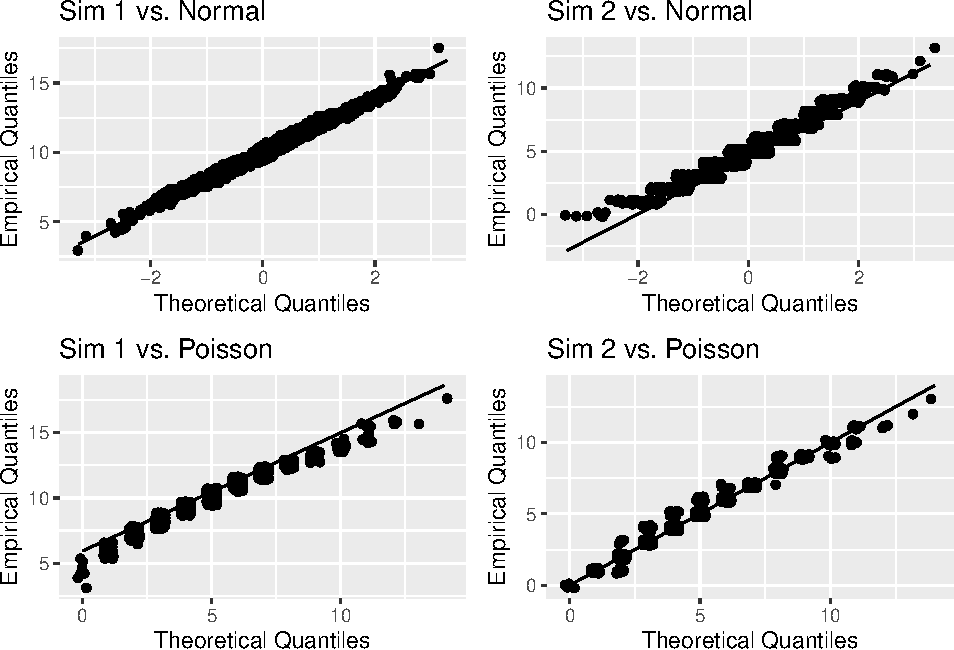
\includegraphics{textbook_files/figure-latex/unnamed-chunk-50-1.pdf} 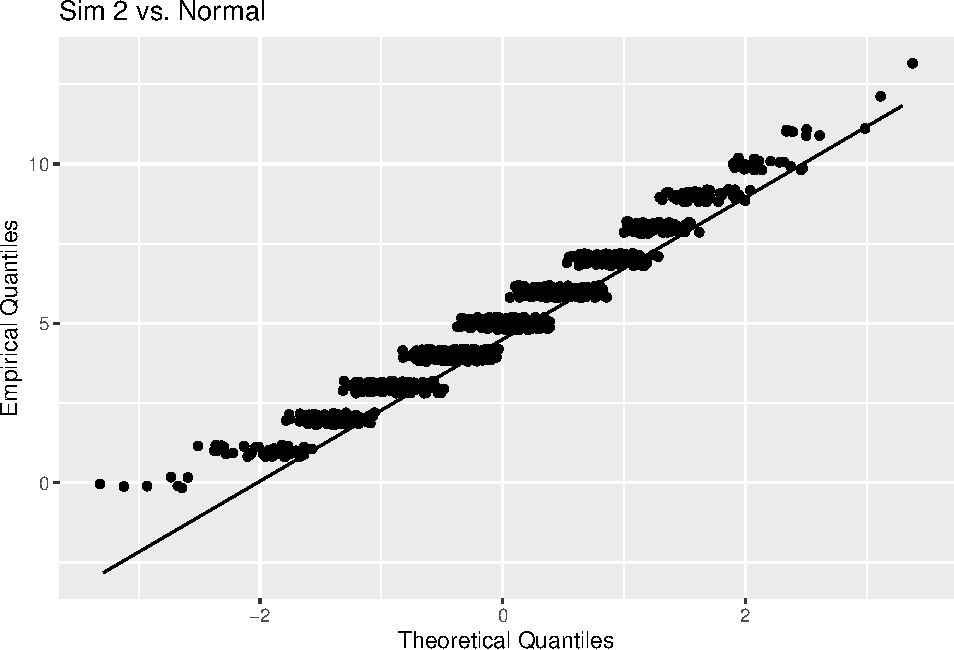
\includegraphics{textbook_files/figure-latex/unnamed-chunk-50-2.pdf} 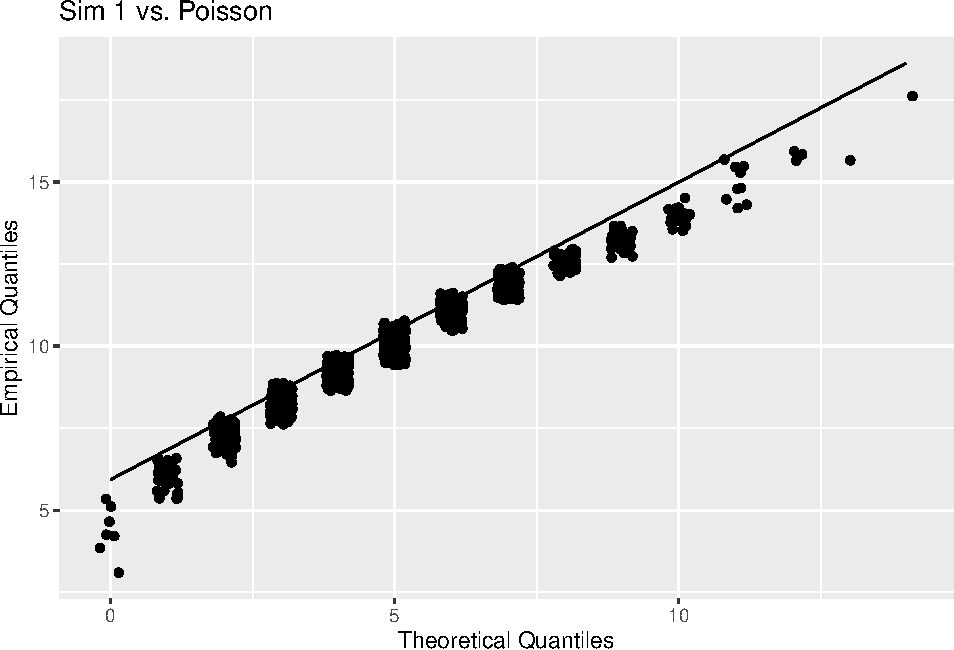
\includegraphics{textbook_files/figure-latex/unnamed-chunk-50-3.pdf} 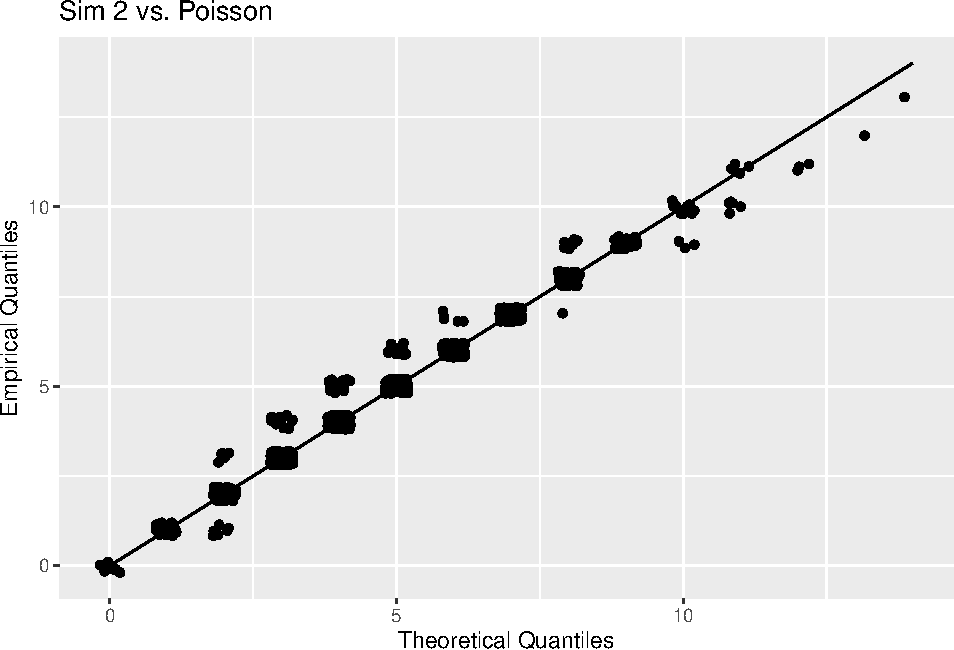
\includegraphics{textbook_files/figure-latex/unnamed-chunk-50-4.pdf}

What do you conclude from the four QQ plots?

\newpage

\hypertarget{common-random-variables}{%
\section{Common Random Variables}\label{common-random-variables}}

There are several families of random variables that show up frequently in applications. Some of these random variables include:
- Binomial
- Geometric
- Poisson
- Normal

\hypertarget{binomial-rvs}{%
\subsection{Binomial RVs}\label{binomial-rvs}}

\begin{definition}
A \textbf{\emph{binomial(n,p) random variable}} is a discrete random variable that counts the numbers of ``successes'' over a fixed number of trials, \(n\), with each trial having an equal probability of success, \(p\).

\(P(X=k) = \binom{n}{k} p^k(1-p)^{n-k} = \frac{n!}{k!\ \cdot\ (n-k)!} p^k(1-p)^{n-k}\), where \(0 \leq k \leq n, 0 \leq p \leq 1\)

If \(X \sim Binomial(n,p)\), then \(E[X]=np\) and \(Var(X)=np(1-p)\)
\end{definition}

\begin{example}
The Cubs and Rockies are playing a 4-game series. The Rockies have a 0.65 probability of winning each game, and the Cubs have a 0.35 probability. Assume each game is independent. Solve for the following quantities.
\end{example}

\begin{enumerate}
\def\labelenumi{(\alph{enumi})}
\item
  The Cubs wins exactly 1 game.\\
  \strut \\
  \strut \\
  \strut \\
\item
  The Rockies win exactly 2 games.\\
  \strut \\
  \strut \\
  \strut \\
\item
  The Cubs win at least 2 games.\\
  \strut \\
  \strut \\
  \strut \\
\item
  The series ends in a sweep.\\
  \strut \\
  \strut \\
  \strut \\
\item
  The expected number of wins for the Rockies.\\
  \strut \\
  \strut \\
  \strut \\
\item
  The variance and standard deviations of wins for the Rockies.\\
  \strut \\
  \strut \\
  \strut \\
\end{enumerate}

\begin{example}
Complete 10,000 simulations of the four game series between the Rockies and Cubs. For the number of Rockies wins, calculate the sample mean and sample variance and compare these to the population values. Also, plot a histogram of the sample data.
\end{example}

\begin{Shaded}
\begin{Highlighting}[]
\FunctionTok{set.seed}\NormalTok{(}\DecValTok{2022}\NormalTok{)}
\NormalTok{rockies\_wins }\OtherTok{\textless{}{-}} \FunctionTok{rbinom}\NormalTok{(}\AttributeTok{n=}\DecValTok{10000}\NormalTok{,}\AttributeTok{size=}\DecValTok{4}\NormalTok{,}\AttributeTok{prob=}\FloatTok{0.65}\NormalTok{)}
\FunctionTok{mean}\NormalTok{(rockies\_wins)}
\end{Highlighting}
\end{Shaded}

\begin{verbatim}
## [1] 2.6036
\end{verbatim}

\begin{Shaded}
\begin{Highlighting}[]
\FunctionTok{var}\NormalTok{(rockies\_wins)}
\end{Highlighting}
\end{Shaded}

\begin{verbatim}
## [1] 0.9121583
\end{verbatim}

\begin{Shaded}
\begin{Highlighting}[]
\NormalTok{rockies\_wins\_df }\OtherTok{\textless{}{-}} \FunctionTok{data.frame}\NormalTok{(}\AttributeTok{Wins=}\NormalTok{rockies\_wins)}
\NormalTok{rockies\_wins\_df }\SpecialCharTok{\%\textgreater{}\%} \FunctionTok{ggplot}\NormalTok{(}\FunctionTok{aes}\NormalTok{(Wins)) }\SpecialCharTok{+} \FunctionTok{geom\_histogram}\NormalTok{(}\AttributeTok{binwidth =} \DecValTok{1}\NormalTok{,}\AttributeTok{color =} \StringTok{"black"}\NormalTok{, }\AttributeTok{fill =} \StringTok{"purple"}\NormalTok{)}
\end{Highlighting}
\end{Shaded}

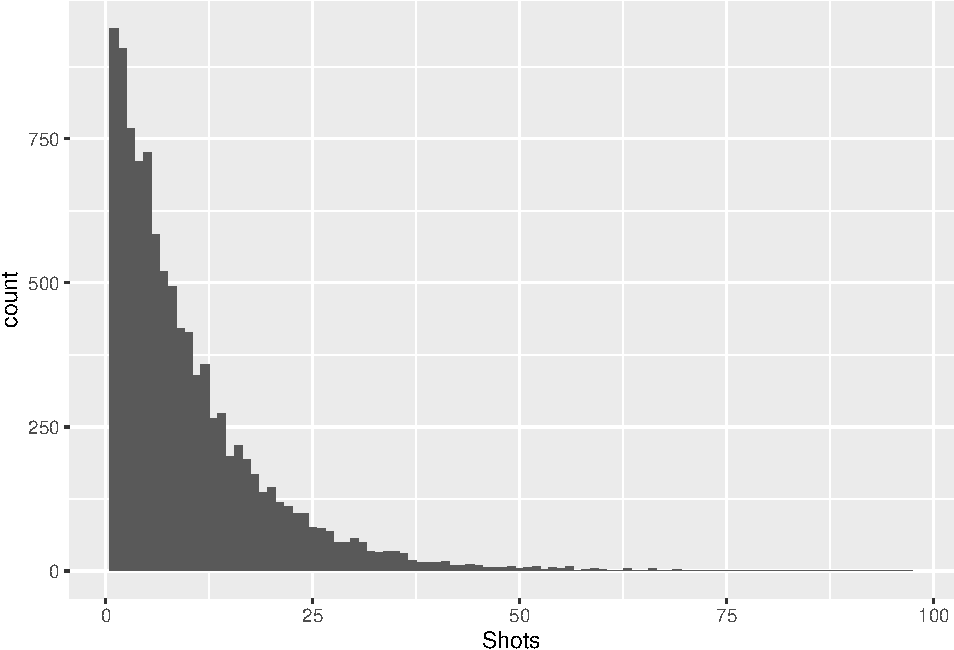
\includegraphics{textbook_files/figure-latex/unnamed-chunk-51-1.pdf}

\hypertarget{binomial-coefficient-symmetry}{%
\subsubsection{Binomial Coefficient Symmetry}\label{binomial-coefficient-symmetry}}

Playoff series for a certain sports league are played as a best-of-seven series, with one team hosting four games and the opposing team hosing three. An executive for the league wishes to know the number of ways the home and away games can be assigned. (One such combination is A-A-B-B-A-B-A, the format used by the NBA and NHL for their best-of-seven series.) What is the total number of combinations?\\
\strut \\
\strut \\
\strut \\

However, instead of thinking about the number of ways to assign the games to the team that gets four home games, what if we thought about the number of ways to assign games to the team that gets three home games?

That would be \(\binom{7}{3}\). We can use the \texttt{choose} command in R to find this quantity.

\begin{Shaded}
\begin{Highlighting}[]
\FunctionTok{choose}\NormalTok{(}\DecValTok{7}\NormalTok{,}\DecValTok{3}\NormalTok{)}
\end{Highlighting}
\end{Shaded}

\begin{verbatim}
## [1] 35
\end{verbatim}

It turns out that this binomial coefficient is also equal to 35.

Theorem: \(\binom{n}{k} = \binom{n}{n-k}\)

\(\binom{n}{k} = \frac{n!}{k!\ \cdot\ (n-k)!}\)

\(\binom{n}{n-k} = \frac{n!}{(n-k)!\ \cdot\ (n-(n-k))!} = \frac{n!}{(n-k)!\ \cdot\ k!} = \binom{n}{k}\)

\newpage

\hypertarget{geometric-rvs}{%
\subsection{Geometric RVs}\label{geometric-rvs}}

\begin{definition}
A \textbf{\emph{Geometric(p) random variable}} is a discrete random variable that counts the numbers of trials until a ``success'' occurs, where the probability of success, \(p\), is constant across all trials.

\(P(X=k) = p(1-p)^{k-1}\), where \(k \geq 1, 0 \leq p \leq 1\)

If \(X \sim Geometric(p)\), then \(E[X]=\frac{1}{p}\) and \(Var(X)=\frac{p}{1-p}\)
\end{definition}

\begin{example}
Suppose the number of shots needed by a hockey team in order to score their first goal, X, is modeled by a Geometric(\(\frac{1}{10}\)) random variable. Use this information to answer the following questions.
\end{example}

\begin{enumerate}
\def\labelenumi{(\alph{enumi})}
\item
  What is the probability that it takes exactly 3 shots to score the first goal?\\
  \strut \\
  \strut \\
  \strut \\
\item
  What is the probability that it takes less than 3 shots to score the first goal?\\
  \strut \\
  \strut \\
  \strut \\
\item
  What is the probability that it takes more than 3 shots to score the first goal?\\
  \strut \\
  \strut \\
  \strut \\
\end{enumerate}

\textbf{Caution:} Some references parameterize the Geometric distribution based on the number of failures before the first success, rather than the trial on which the first success occurs. This changes the PMF, mean, and variance, so be careful.

Let's simulate the number of shot attempts required to score the first goal (Geometric(\(p=1/10\))) from the previous example.

\begin{Shaded}
\begin{Highlighting}[]
\FunctionTok{set.seed}\NormalTok{(}\DecValTok{2022}\NormalTok{)}
\NormalTok{geometric }\OtherTok{\textless{}{-}} \FunctionTok{rgeom}\NormalTok{(}\DecValTok{10000}\NormalTok{, }\DecValTok{1}\SpecialCharTok{/}\DecValTok{10}\NormalTok{)}
\FunctionTok{head}\NormalTok{(geometric, }\DecValTok{20}\NormalTok{)}
\end{Highlighting}
\end{Shaded}

\begin{verbatim}
##  [1]  6 21 26 57 26  1  9  2  8  2  5 13 30 13  9 11  7  8  7 26
\end{verbatim}

Some of the values were 0, which could not happen if R was considering the number of the trial on which the first success occurred. You can add 1 to the values given by \texttt{R} to arrive at the first success distribution.

\begin{Shaded}
\begin{Highlighting}[]
\NormalTok{first\_success }\OtherTok{\textless{}{-}}\NormalTok{ geometric }\SpecialCharTok{+} \DecValTok{1}
\FunctionTok{head}\NormalTok{(first\_success, }\DecValTok{20}\NormalTok{)}
\end{Highlighting}
\end{Shaded}

\begin{verbatim}
##  [1]  7 22 27 58 27  2 10  3  9  3  6 14 31 14 10 12  8  9  8 27
\end{verbatim}

\begin{Shaded}
\begin{Highlighting}[]
\FunctionTok{mean}\NormalTok{(first\_success)}
\end{Highlighting}
\end{Shaded}

\begin{verbatim}
## [1] 10.0588
\end{verbatim}

The mean of this sample of variables is 10.827, which is close to the expected mean of \(\frac{1}{p} = 10\).

Let's plot the sample distribution of shots required to score a goal from the simulation as well.

\begin{Shaded}
\begin{Highlighting}[]
\NormalTok{first\_success\_df }\OtherTok{=} \FunctionTok{data.frame}\NormalTok{(}\AttributeTok{Shots =}\NormalTok{ first\_success)}
\NormalTok{first\_success\_df }\SpecialCharTok{\%\textgreater{}\%} \FunctionTok{ggplot}\NormalTok{(}\FunctionTok{aes}\NormalTok{(}\AttributeTok{x=}\NormalTok{Shots)) }\SpecialCharTok{+} \FunctionTok{geom\_histogram}\NormalTok{(}\AttributeTok{binwidth =} \DecValTok{1}\NormalTok{)}
\end{Highlighting}
\end{Shaded}

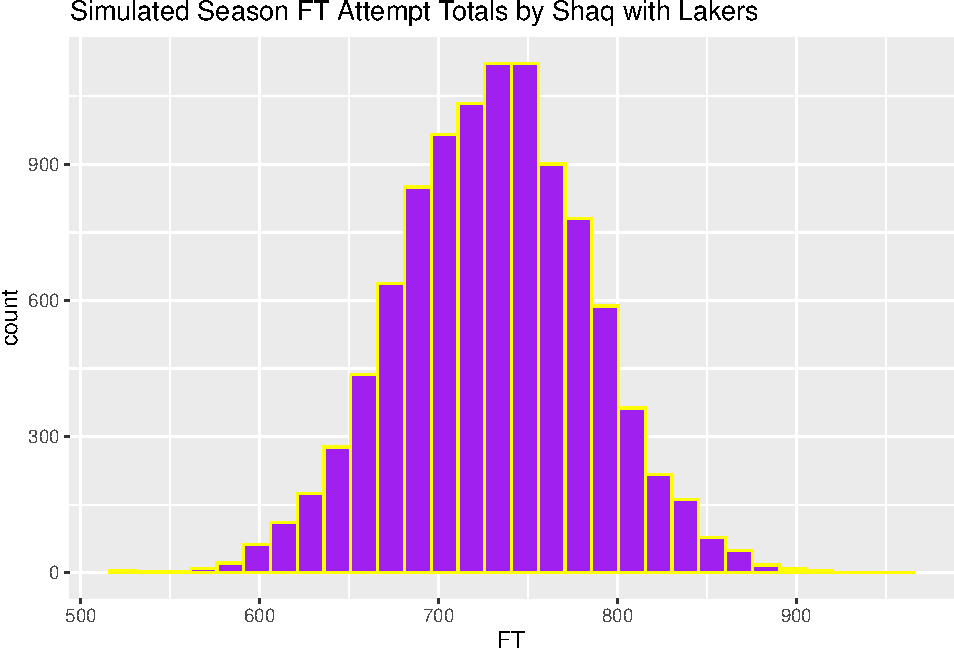
\includegraphics{textbook_files/figure-latex/unnamed-chunk-55-1.pdf}

\newpage

\hypertarget{poisson-rvs}{%
\subsection{Poisson RVs}\label{poisson-rvs}}

\begin{definition}
A \textbf{\emph{Poisson(\(\lambda\)) random variable}} is a discrete random variable that counts the numbers of ``successes'' for a given rate parameter, \(\lambda\), for a given interval.

\(P(X=k) = \frac{e^{-\lambda}\lambda^k}{k!}\), where \(k \geq 0,\)

If \(X \sim Poisson(\lambda)\), then \(E[X]=\lambda\) and \(Var(X)=\lambda\)
\end{definition}

\begin{example}
During the 2021 Major League Soccer season, the Colorado Rapids scored 51 goals in 34 games on their way to a first-place finish in the Western Conference regular season standings.

The team scored \(\frac{51}{34} = 1.5\) goals per game. Let's model the distribution of Rapids goals using a Poisson(1.5) random variable that we'll call Y.
\end{example}

\begin{enumerate}
\def\labelenumi{(\alph{enumi})}
\tightlist
\item
  Which is more likely: Y taking on the value 0 or Y taking on the value 2?\\
  \strut \\
  \strut \\
  \strut \\
\end{enumerate}

We can calculate these probabilities in R using the \texttt{dpois} command.

\begin{Shaded}
\begin{Highlighting}[]
\FunctionTok{dpois}\NormalTok{(}\AttributeTok{x=}\DecValTok{0}\NormalTok{, }\AttributeTok{lambda=}\FloatTok{1.5}\NormalTok{)}
\end{Highlighting}
\end{Shaded}

\begin{verbatim}
## [1] 0.2231302
\end{verbatim}

\begin{Shaded}
\begin{Highlighting}[]
\FunctionTok{dpois}\NormalTok{(}\AttributeTok{x=}\DecValTok{2}\NormalTok{, }\AttributeTok{lambda=}\FloatTok{1.5}\NormalTok{)}
\end{Highlighting}
\end{Shaded}

\begin{verbatim}
## [1] 0.2510214
\end{verbatim}

We can also plot the PMF of Y to check visually.

\begin{Shaded}
\begin{Highlighting}[]
\FunctionTok{ggplot}\NormalTok{(}\FunctionTok{transform}\NormalTok{(}\FunctionTok{data.frame}\NormalTok{(}\AttributeTok{x=}\FunctionTok{c}\NormalTok{(}\DecValTok{0}\SpecialCharTok{:}\DecValTok{8}\NormalTok{)), }\AttributeTok{y=}\FunctionTok{dpois}\NormalTok{(x, }\AttributeTok{lambda =} \FloatTok{1.5}\NormalTok{)), }\FunctionTok{aes}\NormalTok{(x, y)) }\SpecialCharTok{+} 
  \FunctionTok{geom\_bar}\NormalTok{(}\AttributeTok{stat=}\StringTok{"identity"}\NormalTok{) }\SpecialCharTok{+} 
  \FunctionTok{labs}\NormalTok{(}\AttributeTok{x=}\StringTok{"Value"}\NormalTok{, }\AttributeTok{y=}\StringTok{"Frequency"}\NormalTok{, }\AttributeTok{title=}\StringTok{"Probability mass function of Poisson(1.5) random variable"}\NormalTok{)}
\end{Highlighting}
\end{Shaded}

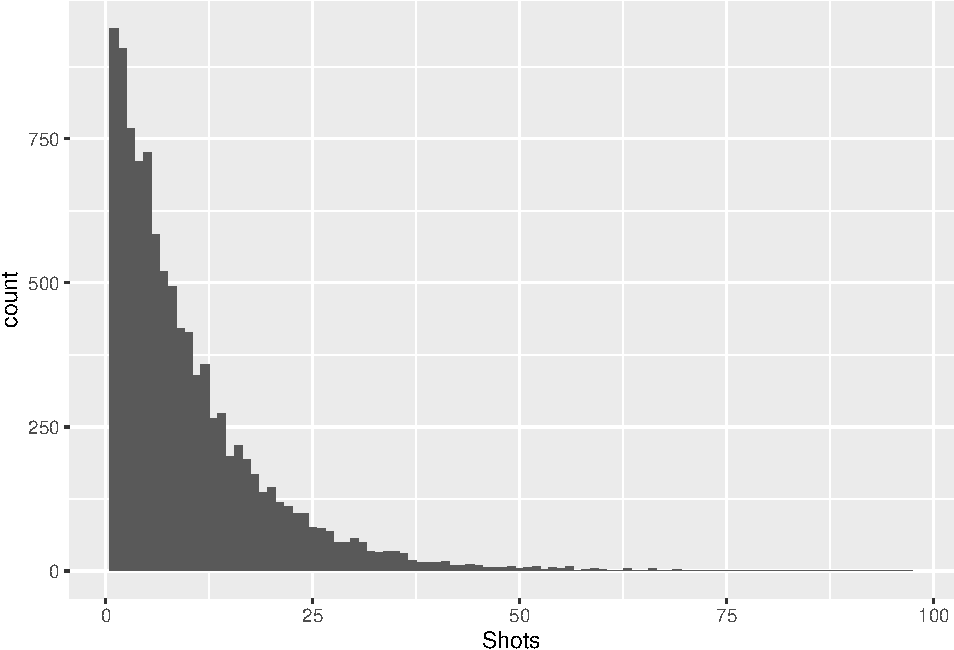
\includegraphics{textbook_files/figure-latex/unnamed-chunk-57-1.pdf}

Let's check whether using a Poisson distribution was appropriate by comparing it to the actual 2021 Colorado Rapids match results.

\begin{Shaded}
\begin{Highlighting}[]
\CommentTok{\# Data: https://www.espn.com/soccer/team/results/\_/id/184/season/2021}

\FunctionTok{library}\NormalTok{(}\StringTok{"kableExtra"}\NormalTok{)}
\NormalTok{rapids21 }\OtherTok{\textless{}{-}} \FunctionTok{c}\NormalTok{(}\DecValTok{0}\NormalTok{,}\DecValTok{1}\NormalTok{,}\DecValTok{1}\NormalTok{,}\DecValTok{3}\NormalTok{,}\DecValTok{3}\NormalTok{,}\DecValTok{1}\NormalTok{,}\DecValTok{3}\NormalTok{,}\DecValTok{2}\NormalTok{,}\DecValTok{1}\NormalTok{,}\DecValTok{1}\NormalTok{,}\DecValTok{2}\NormalTok{,}\DecValTok{1}\NormalTok{,}\DecValTok{2}\NormalTok{,}\DecValTok{0}\NormalTok{,}\DecValTok{1}\NormalTok{,}\DecValTok{0}\NormalTok{,}\DecValTok{3}\NormalTok{,}\DecValTok{2}\NormalTok{,}\DecValTok{2}\NormalTok{,}\DecValTok{1}\NormalTok{,}\DecValTok{1}\NormalTok{,}\DecValTok{1}\NormalTok{,}\DecValTok{2}\NormalTok{,}\DecValTok{1}\NormalTok{,}\DecValTok{0}\NormalTok{,}\DecValTok{3}\NormalTok{,}\DecValTok{0}\NormalTok{,}\DecValTok{3}\NormalTok{,}\DecValTok{1}\NormalTok{,}\DecValTok{1}\NormalTok{,}\DecValTok{2}\NormalTok{,}\DecValTok{0}\NormalTok{,}\DecValTok{1}\NormalTok{,}\DecValTok{5}\NormalTok{)}

\NormalTok{goals }\OtherTok{\textless{}{-}} \FunctionTok{c}\NormalTok{(}\DecValTok{0}\SpecialCharTok{:}\DecValTok{4}\NormalTok{, }\StringTok{"5 or more"}\NormalTok{)}
\NormalTok{actual\_frequency }\OtherTok{\textless{}{-}} \FunctionTok{c}\NormalTok{(}\DecValTok{6}\NormalTok{, }\DecValTok{14}\NormalTok{, }\DecValTok{7}\NormalTok{, }\DecValTok{6}\NormalTok{, }\DecValTok{0}\NormalTok{, }\DecValTok{1}\NormalTok{)}
\NormalTok{actual\_proportion }\OtherTok{\textless{}{-}}\NormalTok{ actual\_frequency }\SpecialCharTok{/} \FunctionTok{sum}\NormalTok{(actual\_frequency)}
\NormalTok{expected\_proportion }\OtherTok{\textless{}{-}} \FunctionTok{c}\NormalTok{(}\FunctionTok{dpois}\NormalTok{(}\DecValTok{0}\SpecialCharTok{:}\DecValTok{4}\NormalTok{, }\AttributeTok{lambda=}\FloatTok{1.5}\NormalTok{), }\FunctionTok{ppois}\NormalTok{(}\DecValTok{4}\NormalTok{, }\AttributeTok{lambda=}\FloatTok{1.5}\NormalTok{, }\AttributeTok{lower.tail=}\ConstantTok{FALSE}\NormalTok{))}
\NormalTok{expected\_frequency }\OtherTok{\textless{}{-}} \FunctionTok{round}\NormalTok{(expected\_proportion }\SpecialCharTok{*} \DecValTok{34}\NormalTok{, }\DecValTok{1}\NormalTok{)}

\NormalTok{rapids.data }\OtherTok{\textless{}{-}} \FunctionTok{data.frame}\NormalTok{(goals, actual\_frequency, actual\_proportion, expected\_frequency, expected\_proportion)}

\NormalTok{rapids.data }\SpecialCharTok{\%\textgreater{}\%}
\FunctionTok{kbl}\NormalTok{() }\SpecialCharTok{\%\textgreater{}\%}
\FunctionTok{kable\_styling}\NormalTok{()}
\end{Highlighting}
\end{Shaded}

\begin{table}
\centering
\begin{tabular}[t]{l|r|r|r|r}
\hline
goals & actual\_frequency & actual\_proportion & expected\_frequency & expected\_proportion\\
\hline
0 & 6 & 0.1764706 & 7.6 & 0.2231302\\
\hline
1 & 14 & 0.4117647 & 11.4 & 0.3346952\\
\hline
2 & 7 & 0.2058824 & 8.5 & 0.2510214\\
\hline
3 & 6 & 0.1764706 & 4.3 & 0.1255107\\
\hline
4 & 0 & 0.0000000 & 1.6 & 0.0470665\\
\hline
5 or more & 1 & 0.0294118 & 0.6 & 0.0185759\\
\hline
\end{tabular}
\end{table}

\begin{enumerate}
\def\labelenumi{(\alph{enumi})}
\setcounter{enumi}{1}
\tightlist
\item
  What differences do you notice between the actual results and the expected values based on the Poisson random variable?\\
  \strut \\
  \strut \\
  \strut \\
\end{enumerate}

\begin{enumerate}
\def\labelenumi{(\alph{enumi})}
\setcounter{enumi}{2}
\tightlist
\item
  Even if the true population distribution of 2021 Rapids goals was truly a Poisson(1.5) random variable, why might the actual distribution of their goals differ from the probability mass function?\\
  \strut \\
  \strut \\
  \strut \\
\end{enumerate}

\begin{enumerate}
\def\labelenumi{(\alph{enumi})}
\setcounter{enumi}{3}
\tightlist
\item
  Use a QQ plot to compare the probability distribution of the 2021 Rapids goals to a Poisson distribution.\\
\end{enumerate}

\begin{Shaded}
\begin{Highlighting}[]
\NormalTok{rapids21 }\SpecialCharTok{\%\textgreater{}\%} 
\NormalTok{  as.data.frame }\SpecialCharTok{\%\textgreater{}\%} 
  \FunctionTok{ggplot}\NormalTok{(}\FunctionTok{aes}\NormalTok{(}\AttributeTok{sample =}\NormalTok{ rapids21)) }\SpecialCharTok{+}
  \FunctionTok{stat\_qq}\NormalTok{(}\AttributeTok{distribution =}\NormalTok{ qpois,}\AttributeTok{dparams =} \FloatTok{1.5}\NormalTok{,}\AttributeTok{position=}\FunctionTok{position\_jitter}\NormalTok{(}\AttributeTok{width =} \FloatTok{0.1}\NormalTok{,}\AttributeTok{height =} \FloatTok{0.1}\NormalTok{)) }\SpecialCharTok{+}
  \FunctionTok{stat\_qq\_line}\NormalTok{(}\AttributeTok{distribution =}\NormalTok{ qpois, }\AttributeTok{dparams =} \FloatTok{1.5}\NormalTok{) }\SpecialCharTok{+}
  \FunctionTok{ggtitle}\NormalTok{(}\StringTok{"QQ{-}plot for Rapids 2021 Goals vs. Poisson Distribution"}\NormalTok{) }\SpecialCharTok{+}
  \FunctionTok{xlab}\NormalTok{(}\StringTok{"Theoretical Quantiles"}\NormalTok{) }\SpecialCharTok{+}
  \FunctionTok{ylab}\NormalTok{(}\StringTok{"Empirical Quantiles"}\NormalTok{)}
\end{Highlighting}
\end{Shaded}

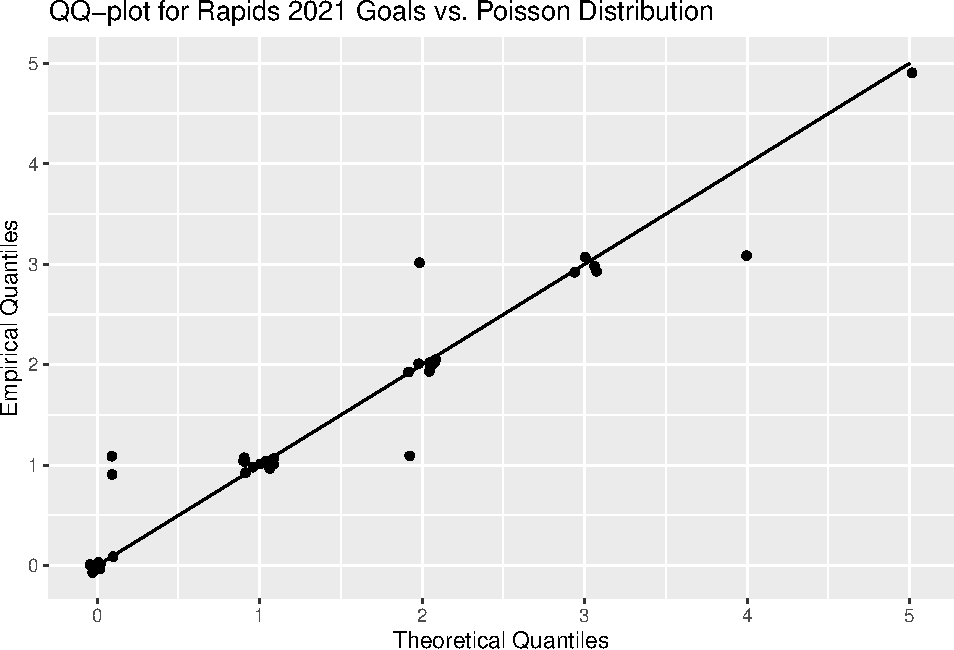
\includegraphics{textbook_files/figure-latex/unnamed-chunk-59-1.pdf}

\begin{enumerate}
\def\labelenumi{(\alph{enumi})}
\setcounter{enumi}{4}
\tightlist
\item
  What are the advantages of using the Poisson distribution to model Major League soccer goals? What are the disadvantages?\\
  \strut \\
  \strut \\
  \strut \\
\end{enumerate}

\begin{example}
In 1997-1998 with the Los Angeles Lakers, Shaquille O'Neal attempted an average of 11.35 free throws per game with a standard deviation of 4.04. Is it appropriate to model Shaq's per game free throw attempts as a Poisson(11.35) random variable?
\end{example}

\begin{enumerate}
\def\labelenumi{(\alph{enumi})}
\tightlist
\item
  Plot the data.
\end{enumerate}

\begin{Shaded}
\begin{Highlighting}[]
\NormalTok{shaq9798 }\OtherTok{\textless{}{-}} \FunctionTok{read\_csv}\NormalTok{(}\StringTok{"data/shaq9798.csv"}\NormalTok{)}
\NormalTok{shaq9798 }\SpecialCharTok{\%\textgreater{}\%} \FunctionTok{ggplot}\NormalTok{(}\FunctionTok{aes}\NormalTok{(}\AttributeTok{x=}\NormalTok{FTA))  }\SpecialCharTok{+} 
  \FunctionTok{geom\_bar}\NormalTok{(}\AttributeTok{color =} \StringTok{"yellow"}\NormalTok{, }\AttributeTok{fill =} \StringTok{"purple"}\NormalTok{) }\SpecialCharTok{+}
  \FunctionTok{ggtitle}\NormalTok{(}\StringTok{"Per Game FT Attempt Totals by Shaq in 1997{-}1998"}\NormalTok{) }\SpecialCharTok{+}
  \FunctionTok{xlim}\NormalTok{(}\DecValTok{0}\NormalTok{,}\DecValTok{25}\NormalTok{)}
\end{Highlighting}
\end{Shaded}

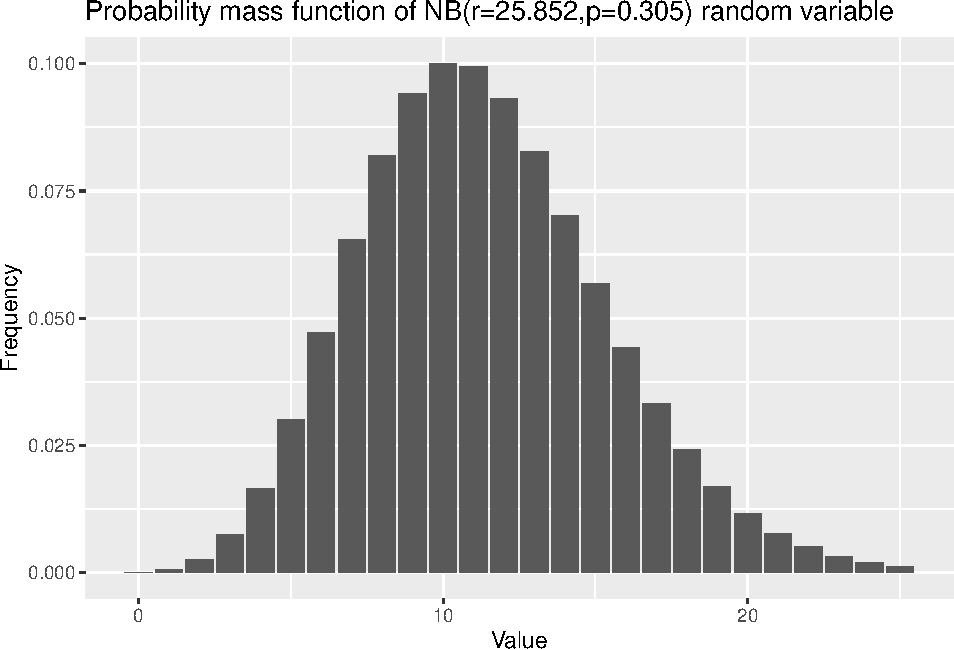
\includegraphics{textbook_files/figure-latex/unnamed-chunk-60-1.pdf}
(b) Plot the PMF of a Poisson(11.35) random variable.

\begin{Shaded}
\begin{Highlighting}[]
\FunctionTok{ggplot}\NormalTok{(}\FunctionTok{transform}\NormalTok{(}\FunctionTok{data.frame}\NormalTok{(}\AttributeTok{x=}\FunctionTok{c}\NormalTok{(}\DecValTok{0}\SpecialCharTok{:}\DecValTok{25}\NormalTok{)), }\AttributeTok{y=}\FunctionTok{dpois}\NormalTok{(x, }\AttributeTok{lambda =} \FloatTok{11.35}\NormalTok{)), }\FunctionTok{aes}\NormalTok{(x, y)) }\SpecialCharTok{+} 
  \FunctionTok{geom\_bar}\NormalTok{(}\AttributeTok{stat=}\StringTok{"identity"}\NormalTok{) }\SpecialCharTok{+} 
  \FunctionTok{labs}\NormalTok{(}\AttributeTok{x=}\StringTok{"Value"}\NormalTok{, }\AttributeTok{y=}\StringTok{"Frequency"}\NormalTok{, }\AttributeTok{title=}\StringTok{"Probability mass function of Poisson(11.35) random variable"}\NormalTok{)}
\end{Highlighting}
\end{Shaded}

\includegraphics{textbook_files/figure-latex/unnamed-chunk-61-1.pdf}

\begin{enumerate}
\def\labelenumi{(\alph{enumi})}
\setcounter{enumi}{2}
\item
  What similarities and what differences do you notice?\\
  \strut \\
  \strut \\
  \strut \\
\item
  Calculate the variance of the two distributions and compare them.
\end{enumerate}

\begin{Shaded}
\begin{Highlighting}[]
\FunctionTok{var}\NormalTok{(shaq9798}\SpecialCharTok{$}\NormalTok{FTA)}
\end{Highlighting}
\end{Shaded}

\begin{verbatim}
## [1] 16.33305
\end{verbatim}

\begin{Shaded}
\begin{Highlighting}[]
\CommentTok{\# Var(Poisson(11.35)) = 11.35}
\end{Highlighting}
\end{Shaded}

\begin{enumerate}
\def\labelenumi{(\alph{enumi})}
\setcounter{enumi}{4}
\tightlist
\item
  Calculate the probability that Shaq had 20 or more free throws and compare it to \(P(Poisson(11.35) \geq 20)\)
\end{enumerate}

\begin{Shaded}
\begin{Highlighting}[]
\NormalTok{shaqFTA }\OtherTok{\textless{}{-}}\NormalTok{ shaq9798}\SpecialCharTok{$}\NormalTok{FTA}
\NormalTok{shaq20 }\OtherTok{\textless{}{-}} \FunctionTok{sum}\NormalTok{(shaqFTA }\SpecialCharTok{\textgreater{}=} \DecValTok{20}\NormalTok{)}\SpecialCharTok{/}\FunctionTok{nrow}\NormalTok{(shaqFTA); shaq20}
\end{Highlighting}
\end{Shaded}

\begin{verbatim}
## numeric(0)
\end{verbatim}

\begin{Shaded}
\begin{Highlighting}[]
\NormalTok{poisson20 }\OtherTok{\textless{}{-}} \FunctionTok{ppois}\NormalTok{(}\DecValTok{20}\NormalTok{, }\AttributeTok{lambda=}\FloatTok{11.35}\NormalTok{, }\AttributeTok{lower.tail=}\ConstantTok{FALSE}\NormalTok{); poisson20}
\end{Highlighting}
\end{Shaded}

\begin{verbatim}
## [1] 0.006536079
\end{verbatim}

\begin{enumerate}
\def\labelenumi{(\alph{enumi})}
\setcounter{enumi}{5}
\tightlist
\item
  Create a QQ-plot of Shaq's per game free throw attempts and a Poisson distribution.
\end{enumerate}

\begin{Shaded}
\begin{Highlighting}[]
\NormalTok{shaq9798 }\SpecialCharTok{\%\textgreater{}\%} 
  \FunctionTok{ggplot}\NormalTok{(}\FunctionTok{aes}\NormalTok{(}\AttributeTok{sample =}\NormalTok{ FTA)) }\SpecialCharTok{+}
  \FunctionTok{stat\_qq}\NormalTok{(}\AttributeTok{distribution =}\NormalTok{ qpois,}\AttributeTok{dparams =} \FloatTok{11.35}\NormalTok{,}\AttributeTok{position=}\FunctionTok{position\_jitter}\NormalTok{(}\AttributeTok{width=}\FloatTok{0.2}\NormalTok{,}\AttributeTok{height=}\FloatTok{0.2}\NormalTok{)) }\SpecialCharTok{+}
  \FunctionTok{stat\_qq\_line}\NormalTok{(}\AttributeTok{distribution =}\NormalTok{ qpois, }\AttributeTok{dparams =} \FloatTok{11.35}\NormalTok{) }\SpecialCharTok{+}
  \FunctionTok{ggtitle}\NormalTok{(}\StringTok{"QQ{-}plot for Shaq\textquotesingle{}s Free Throw Attempts vs. Poisson Distribution"}\NormalTok{) }\SpecialCharTok{+}
  \FunctionTok{xlab}\NormalTok{(}\StringTok{"Theoretical Quantiles"}\NormalTok{) }\SpecialCharTok{+}
  \FunctionTok{ylab}\NormalTok{(}\StringTok{"Empirical Quantiles"}\NormalTok{)}
\end{Highlighting}
\end{Shaded}

\includegraphics{textbook_files/figure-latex/unnamed-chunk-64-1.pdf}

\begin{enumerate}
\def\labelenumi{(\alph{enumi})}
\setcounter{enumi}{6}
\tightlist
\item
  Is the Poisson distribution appropriate to model Shaq's FTA per game? Explain.\\
  \strut \\
  \strut \\
  \strut \\
\end{enumerate}

\newpage

\hypertarget{negative-binomial-rvs}{%
\subsection{Negative Binomial RVs}\label{negative-binomial-rvs}}

\begin{definition}
A \textbf{\emph{Negative Binomial(\(r\),\(p\)) random variable}} is a discrete random variable that counts the numbers of ``successes'' for given parameters, \(r\) and \(p\).

\(P(X=k) = {k+r-1 \choose k}(1-p)^rp^k\), where \(k \geq 0,\)

If \(X \sim NB(r,p)\), then \(E[X]=\frac{rp}{1-p}\) and \(Var(X)=\frac{rp}{(1-p)^2}\)
\end{definition}

The Negative Binomial distribution is often used to model count data that is ``overdispersed''. A property of the Poisson distribution is that the mean and variance are equal. If you are analyzing count data such that the variance is much greater than the mean (i.e., overdispersed), then the Negative Binomial distribution may be an appropriate substitute.

Given sample count data, we can estimate appropriate parameters for a Negative Binomial in many ways. One such way is to use the ``method of moments'' estimator.

These estimators are given by:

\(\hat{p} = \frac{s^2-\bar{x}}{s^2}\) and \(\hat{r} = \frac{\bar{x}^2}{s^2-\bar{x}}\)

\begin{example}
Using Shaq's 1997-1998 data, model his per game free throw attempts as a Negative Binomial random variable.
\end{example}

\begin{enumerate}
\def\labelenumi{(\alph{enumi})}
\tightlist
\item
  Find an appropriate choice of parameters, \(r\) and \(p\).
\end{enumerate}

\begin{Shaded}
\begin{Highlighting}[]
\NormalTok{shaq.mean }\OtherTok{\textless{}{-}} \FunctionTok{mean}\NormalTok{(shaqFTA)}
\NormalTok{shaq.var }\OtherTok{\textless{}{-}} \FunctionTok{var}\NormalTok{(shaqFTA)}
\NormalTok{rhat }\OtherTok{\textless{}{-}}\NormalTok{ shaq.mean}\SpecialCharTok{\^{}}\DecValTok{2}\SpecialCharTok{/}\NormalTok{(shaq.var}\SpecialCharTok{{-}}\NormalTok{shaq.mean)}
\NormalTok{phat }\OtherTok{\textless{}{-}}\NormalTok{ (shaq.var}\SpecialCharTok{{-}}\NormalTok{shaq.mean)}\SpecialCharTok{/}\NormalTok{shaq.var}
\FunctionTok{c}\NormalTok{(rhat,phat)}
\end{Highlighting}
\end{Shaded}

\begin{verbatim}
## [1] 25.85213  0.30509
\end{verbatim}

\begin{enumerate}
\def\labelenumi{(\alph{enumi})}
\setcounter{enumi}{1}
\tightlist
\item
  Plot the Negative Binomial distribution. Note that R uses an alternative parameterization for \(p\). Use \(prob = 1-p\).
\end{enumerate}

\begin{Shaded}
\begin{Highlighting}[]
\FunctionTok{ggplot}\NormalTok{(}\FunctionTok{transform}\NormalTok{(}\FunctionTok{data.frame}\NormalTok{(}\AttributeTok{x=}\FunctionTok{c}\NormalTok{(}\DecValTok{0}\SpecialCharTok{:}\DecValTok{25}\NormalTok{)), }\AttributeTok{y=}\FunctionTok{dnbinom}\NormalTok{(x,}\AttributeTok{size=}\NormalTok{rhat,}\AttributeTok{prob=}\DecValTok{1}\SpecialCharTok{{-}}\NormalTok{phat)), }\FunctionTok{aes}\NormalTok{(x, y)) }\SpecialCharTok{+} 
  \FunctionTok{geom\_bar}\NormalTok{(}\AttributeTok{stat=}\StringTok{"identity"}\NormalTok{) }\SpecialCharTok{+} 
  \FunctionTok{labs}\NormalTok{(}\AttributeTok{x=}\StringTok{"Value"}\NormalTok{, }\AttributeTok{y=}\StringTok{"Frequency"}\NormalTok{, }\AttributeTok{title=}\StringTok{"Probability mass function of NB(r=25.852,p=0.305) random variable"}\NormalTok{)}
\end{Highlighting}
\end{Shaded}

\includegraphics{textbook_files/figure-latex/unnamed-chunk-66-1.pdf}

\begin{enumerate}
\def\labelenumi{(\alph{enumi})}
\setcounter{enumi}{2}
\tightlist
\item
  Calculate the mean and variance of the Negative Binomial and Shaq's dataset.
\end{enumerate}

\begin{Shaded}
\begin{Highlighting}[]
\NormalTok{shaq.mean }\OtherTok{\textless{}{-}} \FunctionTok{mean}\NormalTok{(shaqFTA)}
\NormalTok{shaq.var }\OtherTok{\textless{}{-}} \FunctionTok{var}\NormalTok{(shaqFTA)}
\NormalTok{NB.mean }\OtherTok{\textless{}{-}}\NormalTok{ (rhat}\SpecialCharTok{*}\NormalTok{phat)}\SpecialCharTok{/}\NormalTok{(}\DecValTok{1}\SpecialCharTok{{-}}\NormalTok{phat)}
\NormalTok{NB.var }\OtherTok{\textless{}{-}}\NormalTok{ (rhat}\SpecialCharTok{*}\NormalTok{phat)}\SpecialCharTok{/}\NormalTok{(}\DecValTok{1}\SpecialCharTok{{-}}\NormalTok{phat)}\SpecialCharTok{\^{}}\DecValTok{2}
\FunctionTok{c}\NormalTok{(shaq.mean,shaq.var)}
\end{Highlighting}
\end{Shaded}

\begin{verbatim}
## [1] 11.35000 16.33305
\end{verbatim}

\begin{Shaded}
\begin{Highlighting}[]
\FunctionTok{c}\NormalTok{(NB.mean,NB.var)}
\end{Highlighting}
\end{Shaded}

\begin{verbatim}
## [1] 11.35000 16.33305
\end{verbatim}

\begin{enumerate}
\def\labelenumi{(\alph{enumi})}
\setcounter{enumi}{3}
\tightlist
\item
  Calculate the probability that Shaq had 20 or more free throws and compare it to \(P(NB(r=25.852,p=0.305) \geq 20)\)
\end{enumerate}

\begin{Shaded}
\begin{Highlighting}[]
\NormalTok{shaq20 }\OtherTok{\textless{}{-}} \FunctionTok{sum}\NormalTok{(shaqFTA }\SpecialCharTok{\textgreater{}=} \DecValTok{20}\NormalTok{)}\SpecialCharTok{/}\FunctionTok{nrow}\NormalTok{(shaqFTA); shaq20}
\end{Highlighting}
\end{Shaded}

\begin{verbatim}
## numeric(0)
\end{verbatim}

\begin{Shaded}
\begin{Highlighting}[]
\NormalTok{nb20 }\OtherTok{\textless{}{-}} \FunctionTok{pnbinom}\NormalTok{(}\DecValTok{20}\NormalTok{,}\AttributeTok{size=}\NormalTok{rhat,}\AttributeTok{prob=}\DecValTok{1}\SpecialCharTok{{-}}\NormalTok{phat,}\AttributeTok{lower.tail=}\ConstantTok{FALSE}\NormalTok{); nb20}
\end{Highlighting}
\end{Shaded}

\begin{verbatim}
## [1] 0.0208711
\end{verbatim}

\begin{enumerate}
\def\labelenumi{(\alph{enumi})}
\setcounter{enumi}{4}
\tightlist
\item
  Create a QQ-plot of Shaq's per game free throw attempts and a Negative Binomial distribution.
\end{enumerate}

\begin{Shaded}
\begin{Highlighting}[]
\NormalTok{shaq9798 }\SpecialCharTok{\%\textgreater{}\%} 
  \FunctionTok{ggplot}\NormalTok{(}\FunctionTok{aes}\NormalTok{(}\AttributeTok{sample =}\NormalTok{ FTA)) }\SpecialCharTok{+}
  \FunctionTok{stat\_qq}\NormalTok{(}\AttributeTok{distribution =}\NormalTok{ qnbinom,}\AttributeTok{dparams =} \FunctionTok{list}\NormalTok{(}\AttributeTok{size=}\FloatTok{25.852}\NormalTok{,}\AttributeTok{mu=}\FloatTok{11.35}\NormalTok{),}\AttributeTok{position=}\FunctionTok{position\_jitter}\NormalTok{(}\AttributeTok{width=}\FloatTok{0.2}\NormalTok{,}\AttributeTok{height=}\FloatTok{0.2}\NormalTok{)) }\SpecialCharTok{+}
  \FunctionTok{stat\_qq\_line}\NormalTok{(}\AttributeTok{distribution =}\NormalTok{ qnbinom, }\AttributeTok{dparams =} \FunctionTok{list}\NormalTok{(}\AttributeTok{size=}\FloatTok{25.852}\NormalTok{,}\AttributeTok{mu=}\FloatTok{11.35}\NormalTok{)) }\SpecialCharTok{+}
  \FunctionTok{ggtitle}\NormalTok{(}\StringTok{"QQ{-}plot for Shaq\textquotesingle{}s Free Throw Attempts vs. Neaative Binomial Distribution"}\NormalTok{) }\SpecialCharTok{+}
  \FunctionTok{xlab}\NormalTok{(}\StringTok{"Theoretical Quantiles"}\NormalTok{) }\SpecialCharTok{+}
  \FunctionTok{ylab}\NormalTok{(}\StringTok{"Empirical Quantiles"}\NormalTok{)}
\end{Highlighting}
\end{Shaded}

\includegraphics{textbook_files/figure-latex/unnamed-chunk-69-1.pdf}

\begin{enumerate}
\def\labelenumi{(\alph{enumi})}
\setcounter{enumi}{5}
\tightlist
\item
  Is the Negative Binomial distribution appropriate to model Shaq's FTA per game? How does it compare to using the Poisson distribution? Explain.\\
  \strut \\
  \strut \\
  \strut \\
\end{enumerate}

\newpage

\hypertarget{normal-rvs}{%
\subsection{Normal RVs}\label{normal-rvs}}

\begin{definition}
A \textbf{\emph{Normal(\(\mu\),\(\sigma^2\)) random variable}} is a continuous random variable that is bell-shaped with mean \(\mu\) and variance \(\sigma^2\).

To calculate probabilities under the normal curve, you need either to integrate, use a table, or a computer.

Note that a normal random variable can be standardized by using: \(z = \frac{x-\mu}{\sigma}\)
\end{definition}

\begin{theorem}
For a normal(\(\mu\),\(\sigma^2\)) random variable, we have the following approximations:\\
- About 68\% of the data falls within one standard deviation of the mean (i.e., \(\mu \pm \sigma\))\\
- About 95\% of the data falls within two standard deviations of the mean (i.e., \(\mu \pm 2\sigma\))\\
- About 99.7\% of the data falls within three standard deviations of the mean (i.e., \(\mu \pm 3\sigma\))
\end{theorem}

\begin{example}
The skills (or tools) of a baseball player are often rated on a scale of 20-80, where 50 is an average grade, 20 is the lowest grade, and 80 is the highest grade. The distribution of tool grades is approximately normally distributed (\(\mu=50, \sigma =10\)).

See \url{https://blogs.fangraphs.com/scouting-explained-the-20-80-scouting-scale/} for more details. Calculate the following probabilities.
\end{example}

\begin{enumerate}
\def\labelenumi{(\alph{enumi})}
\item
  Former Rockie Nolan Arenado has been graded to have game power of 70. Game power estimates a player's ability to hit home runs. Approximately what percentage of baseball players have equal or greater game power than Arenado?\\
  \strut \\
  \strut \\
  \strut \\
\item
  Mike Trout has been graded to have raw power of 55. Raw power estimates a player's ability to hit baseballs hard (i.e., hard hit rate). Approximately what percentage of baseball players have equal or less raw power than Arenado?\\
  \strut \\
  \strut \\
  \strut \\
\item
  Suppose a Rockies prospect is said to be in the top 10\% of all baseball players in terms of their speed. What approximate speed grade would correspond to the player?\\
  \strut \\
  \strut \\
  \strut \\
\item
  Suppose a Rockies prospect is said to be in the bottom 20\% of all baseball players in terms of their hit ability. What approximate hit grade would correspond to the player?\\
  \strut \\
  \strut \\
  \strut \\
\item
  Between what two grades do approximately 95\% of all players lie for a given tool?\\
  \strut \\
  \strut \\
  \strut \\
\end{enumerate}

Let's check our answers:

\begin{Shaded}
\begin{Highlighting}[]
\NormalTok{a }\OtherTok{\textless{}{-}} \DecValTok{1}\SpecialCharTok{{-}}\FunctionTok{pnorm}\NormalTok{(}\AttributeTok{q=}\DecValTok{70}\NormalTok{,}\AttributeTok{mean=}\DecValTok{50}\NormalTok{,}\AttributeTok{sd=}\DecValTok{10}\NormalTok{); a}
\end{Highlighting}
\end{Shaded}

\begin{verbatim}
## [1] 0.02275013
\end{verbatim}

\begin{Shaded}
\begin{Highlighting}[]
\NormalTok{b }\OtherTok{\textless{}{-}} \FunctionTok{pnorm}\NormalTok{(}\AttributeTok{q=}\DecValTok{55}\NormalTok{,}\AttributeTok{mean=}\DecValTok{50}\NormalTok{,}\AttributeTok{sd=}\DecValTok{10}\NormalTok{); b}
\end{Highlighting}
\end{Shaded}

\begin{verbatim}
## [1] 0.6914625
\end{verbatim}

\begin{Shaded}
\begin{Highlighting}[]
\NormalTok{c }\OtherTok{\textless{}{-}} \FunctionTok{qnorm}\NormalTok{(}\FloatTok{0.1}\NormalTok{,}\AttributeTok{mean=}\DecValTok{50}\NormalTok{,}\AttributeTok{sd=}\DecValTok{10}\NormalTok{,}\AttributeTok{lower.tail =}\NormalTok{ F); c}
\end{Highlighting}
\end{Shaded}

\begin{verbatim}
## [1] 62.81552
\end{verbatim}

\begin{Shaded}
\begin{Highlighting}[]
\NormalTok{d }\OtherTok{\textless{}{-}} \FunctionTok{qnorm}\NormalTok{(}\FloatTok{0.2}\NormalTok{,}\AttributeTok{mean=}\DecValTok{50}\NormalTok{,}\AttributeTok{sd=}\DecValTok{10}\NormalTok{,}\AttributeTok{lower.tail =}\NormalTok{ T); d}
\end{Highlighting}
\end{Shaded}

\begin{verbatim}
## [1] 41.58379
\end{verbatim}

\begin{Shaded}
\begin{Highlighting}[]
\NormalTok{e }\OtherTok{\textless{}{-}} \FunctionTok{pnorm}\NormalTok{(}\AttributeTok{q=}\DecValTok{70}\NormalTok{,}\AttributeTok{mean=}\DecValTok{50}\NormalTok{,}\AttributeTok{sd=}\DecValTok{10}\NormalTok{) }\SpecialCharTok{{-}} \FunctionTok{pnorm}\NormalTok{(}\AttributeTok{q=}\DecValTok{30}\NormalTok{,}\AttributeTok{mean=}\DecValTok{50}\NormalTok{,}\AttributeTok{sd=}\DecValTok{10}\NormalTok{); e}
\end{Highlighting}
\end{Shaded}

\begin{verbatim}
## [1] 0.9544997
\end{verbatim}

\newpage

\begin{example}
Player X has a projected mean WAR of 3 with standard deviation of 2 and player Y has a projected mean WAR of 1.5 with a standard deviation of 3. Assume projected WAR is normally distributed. What is the probability that Player X outperforms Player Y?

Link to WAR explaination: \url{https://www.mlb.com/glossary/advanced-stats/wins-above-replacement}
\end{example}

We want Pr(X\textgreater Y) or Pr(X-Y\textgreater0).\\
Let Z = X-Y.\\
E{[}Z{]}=1.5
Var(Z)=5
Pr(Z\textgreater0)=1-Pr(Z \(\leq\) 0)

\begin{Shaded}
\begin{Highlighting}[]
\CommentTok{\#Calculate probability Z\textless{}=0}
\NormalTok{pr }\OtherTok{\textless{}{-}} \FunctionTok{pnorm}\NormalTok{(}\DecValTok{0}\NormalTok{,}\FloatTok{1.5}\NormalTok{,}\FunctionTok{sqrt}\NormalTok{(}\DecValTok{5}\NormalTok{))}
\FunctionTok{print}\NormalTok{(}\DecValTok{1}\SpecialCharTok{{-}}\NormalTok{pr)}
\end{Highlighting}
\end{Shaded}

\begin{verbatim}
## [1] 0.7488325
\end{verbatim}

The Probability that Player X outperforms Player Y is 0.7488.

\newpage

\hypertarget{case-study-nfl-state-values-and-decision-making}{%
\section{Case Study: NFL state values and decision making}\label{case-study-nfl-state-values-and-decision-making}}

(Mathletics, chapter 19-20, page 170)

\hypertarget{monte-carlo-simulation}{%
\chapter{Monte Carlo Simulation}\label{monte-carlo-simulation}}

\hypertarget{basics}{%
\section{Basics}\label{basics}}

Monte Carlo Simulation is a collection of computer-driven, computational algorithms that use repeated random sampling to calculate estimates. The basic steps for such a simulation are as follows:

\begin{enumerate}
\def\labelenumi{\arabic{enumi})}
\item
  Set seed for replicability
\item
  Initialize all variables/vectors
\item
  Loop through ``n'' simulations and save simulated values
\item
  Analyze the simulated values from the ``n'' simulations
\end{enumerate}

One function that will be particularly useful for simulation is \texttt{set.seed()}.

\texttt{set.seed()} allows us to replicate any simulation by giving the initial seed for the simulation. The actual number that is ``seeded'' is not particularly important though if you want to replicate the same simulations, you will want to re-use this number.

\newpage

\begin{example}
Simulate 10 overtime coin tosses with and without using \texttt{set.seed()} and compare the results
\end{example}

\begin{Shaded}
\begin{Highlighting}[]
\CommentTok{\# Sample 1}
\FunctionTok{sample}\NormalTok{(}\FunctionTok{c}\NormalTok{(}\StringTok{"H"}\NormalTok{,}\StringTok{"T"}\NormalTok{),}\AttributeTok{size=}\DecValTok{10}\NormalTok{,}\AttributeTok{prob=}\FunctionTok{c}\NormalTok{(}\FloatTok{0.5}\NormalTok{,}\FloatTok{0.5}\NormalTok{),}\AttributeTok{replace=}\NormalTok{T)}
\end{Highlighting}
\end{Shaded}

\begin{verbatim}
##  [1] "T" "H" "T" "T" "T" "H" "H" "H" "T" "T"
\end{verbatim}

\begin{Shaded}
\begin{Highlighting}[]
\CommentTok{\# Sample 2}
\FunctionTok{sample}\NormalTok{(}\FunctionTok{c}\NormalTok{(}\StringTok{"H"}\NormalTok{,}\StringTok{"T"}\NormalTok{),}\AttributeTok{size=}\DecValTok{10}\NormalTok{,}\AttributeTok{prob=}\FunctionTok{c}\NormalTok{(}\FloatTok{0.5}\NormalTok{,}\FloatTok{0.5}\NormalTok{),}\AttributeTok{replace=}\NormalTok{T)}
\end{Highlighting}
\end{Shaded}

\begin{verbatim}
##  [1] "T" "H" "T" "T" "H" "H" "H" "H" "T" "T"
\end{verbatim}

\begin{Shaded}
\begin{Highlighting}[]
\CommentTok{\# Sample 3}
\FunctionTok{set.seed}\NormalTok{(}\DecValTok{2020}\NormalTok{)}
\FunctionTok{sample}\NormalTok{(}\FunctionTok{c}\NormalTok{(}\StringTok{"H"}\NormalTok{,}\StringTok{"T"}\NormalTok{),}\AttributeTok{size=}\DecValTok{10}\NormalTok{,}\AttributeTok{prob=}\FunctionTok{c}\NormalTok{(}\FloatTok{0.5}\NormalTok{,}\FloatTok{0.5}\NormalTok{),}\AttributeTok{replace=}\NormalTok{T)}
\end{Highlighting}
\end{Shaded}

\begin{verbatim}
##  [1] "H" "T" "H" "T" "T" "T" "T" "T" "T" "H"
\end{verbatim}

\begin{Shaded}
\begin{Highlighting}[]
\CommentTok{\# Sample 4}
\FunctionTok{set.seed}\NormalTok{(}\DecValTok{2020}\NormalTok{)}
\FunctionTok{sample}\NormalTok{(}\FunctionTok{c}\NormalTok{(}\StringTok{"H"}\NormalTok{,}\StringTok{"T"}\NormalTok{),}\AttributeTok{size=}\DecValTok{10}\NormalTok{,}\AttributeTok{prob=}\FunctionTok{c}\NormalTok{(}\FloatTok{0.5}\NormalTok{,}\FloatTok{0.5}\NormalTok{),}\AttributeTok{replace=}\NormalTok{T)}
\end{Highlighting}
\end{Shaded}

\begin{verbatim}
##  [1] "H" "T" "H" "T" "T" "T" "T" "T" "T" "H"
\end{verbatim}

Simulation can be very helpful when you want to estimate quantities that are not easily solved using analytical methods like formulas.

\newpage

\begin{example}
Shaquille O'Neal has a career free throw percentage of 52.7\%. Suppose that Shaq takes 10 free throw shots. What is the probability that he makes all 10 shots?
\end{example}

In this case, we can calculate the exact probability of interest using binomial random variable.

\begin{Shaded}
\begin{Highlighting}[]
\FunctionTok{dbinom}\NormalTok{(}\AttributeTok{x=}\DecValTok{10}\NormalTok{,}\AttributeTok{size=}\DecValTok{10}\NormalTok{,}\AttributeTok{prob=}\FloatTok{0.527}\NormalTok{)}
\end{Highlighting}
\end{Shaded}

\begin{verbatim}
## [1] 0.001652366
\end{verbatim}

In more complicated simulations, there may not be an easy formula to use to calculate the value of interest. In these situations, simulation can be very helpful in estimating quantities.

\begin{Shaded}
\begin{Highlighting}[]
\FunctionTok{set.seed}\NormalTok{(}\DecValTok{2020}\NormalTok{)}

\CommentTok{\# Number of Simulations}
\NormalTok{n.sims }\OtherTok{\textless{}{-}} \DecValTok{10000}

\CommentTok{\# Initialize FT variable with 10000 zeros}
\NormalTok{FT }\OtherTok{\textless{}{-}} \FunctionTok{rep}\NormalTok{(}\DecValTok{0}\NormalTok{,n.sims)}

\ControlFlowTok{for}\NormalTok{(i }\ControlFlowTok{in} \DecValTok{1}\SpecialCharTok{:}\NormalTok{n.sims)\{}
  \CommentTok{\# Simulate 10 free throws}
\NormalTok{  temp }\OtherTok{\textless{}{-}} \FunctionTok{sample}\NormalTok{(}\AttributeTok{x=}\FunctionTok{c}\NormalTok{(}\DecValTok{0}\NormalTok{,}\DecValTok{1}\NormalTok{), }\AttributeTok{size =} \DecValTok{10}\NormalTok{, }\AttributeTok{replace =}\NormalTok{ T, }\AttributeTok{prob =} \FunctionTok{c}\NormalTok{(}\FloatTok{0.473}\NormalTok{,}\FloatTok{0.527}\NormalTok{) )}
  
  \CommentTok{\# Count the number of free throws made and store them in FT}
\NormalTok{  FT[i] }\OtherTok{\textless{}{-}} \FunctionTok{sum}\NormalTok{(temp)}
\NormalTok{\}}

\NormalTok{FT }\SpecialCharTok{\%\textgreater{}\%} 
  \FunctionTok{as.data.frame}\NormalTok{() }\SpecialCharTok{\%\textgreater{}\%} 
  \FunctionTok{ggplot}\NormalTok{(}\FunctionTok{aes}\NormalTok{(}\AttributeTok{x=}\NormalTok{FT)) }\SpecialCharTok{+} 
  \FunctionTok{geom\_bar}\NormalTok{() }\SpecialCharTok{+}
  \FunctionTok{ggtitle}\NormalTok{(}\StringTok{"Number of free throws made out of 10"}\NormalTok{) }\SpecialCharTok{+} 
  \FunctionTok{scale\_x\_continuous}\NormalTok{(}\AttributeTok{breaks =} \FunctionTok{seq}\NormalTok{(}\DecValTok{0}\NormalTok{, }\DecValTok{10}\NormalTok{, }\AttributeTok{by =} \DecValTok{2}\NormalTok{))}
\end{Highlighting}
\end{Shaded}

\includegraphics{textbook_files/figure-latex/unnamed-chunk-76-1.pdf}

\begin{Shaded}
\begin{Highlighting}[]
\NormalTok{prob10 }\OtherTok{\textless{}{-}} \FunctionTok{sum}\NormalTok{(FT }\SpecialCharTok{==} \DecValTok{10}\NormalTok{)}\SpecialCharTok{/}\NormalTok{n.sims; prob10}
\end{Highlighting}
\end{Shaded}

\begin{verbatim}
## [1] 0.0023
\end{verbatim}

\begin{Shaded}
\begin{Highlighting}[]
\NormalTok{prob10 }\OtherTok{\textless{}{-}} \FunctionTok{mean}\NormalTok{(FT }\SpecialCharTok{==} \DecValTok{10}\NormalTok{); prob10}
\end{Highlighting}
\end{Shaded}

\begin{verbatim}
## [1] 0.0023
\end{verbatim}

The estimated probability that Shaq goes 10-for-10 in free throw attempts based on his career average is 0.0023.

If we run the simulation again with a different seed, we will get another estimate (0.0019).

\begin{Shaded}
\begin{Highlighting}[]
\FunctionTok{set.seed}\NormalTok{(}\DecValTok{1}\NormalTok{)}

\CommentTok{\# Number of Simulations}
\NormalTok{n.sims }\OtherTok{\textless{}{-}} \DecValTok{10000}

\CommentTok{\# Initialize FT variable with 10000 zeros}
\NormalTok{FT }\OtherTok{\textless{}{-}} \FunctionTok{rep}\NormalTok{(}\DecValTok{0}\NormalTok{,n.sims)}

\ControlFlowTok{for}\NormalTok{(i }\ControlFlowTok{in} \DecValTok{1}\SpecialCharTok{:}\NormalTok{n.sims)\{}
  \CommentTok{\# Simulate 10 free throws}
\NormalTok{  temp }\OtherTok{\textless{}{-}} \FunctionTok{sample}\NormalTok{(}\AttributeTok{x=}\FunctionTok{c}\NormalTok{(}\DecValTok{0}\NormalTok{,}\DecValTok{1}\NormalTok{), }\AttributeTok{size =} \DecValTok{10}\NormalTok{, }\AttributeTok{replace =}\NormalTok{ T, }\AttributeTok{prob =} \FunctionTok{c}\NormalTok{(}\FloatTok{0.473}\NormalTok{,}\FloatTok{0.527}\NormalTok{) )}
  
  \CommentTok{\# Count the number of free throws made and store them in FT}
\NormalTok{  FT[i] }\OtherTok{\textless{}{-}} \FunctionTok{sum}\NormalTok{(temp)}
\NormalTok{\}}

\NormalTok{prob10 }\OtherTok{\textless{}{-}} \FunctionTok{mean}\NormalTok{(FT }\SpecialCharTok{==} \DecValTok{10}\NormalTok{); prob10}
\end{Highlighting}
\end{Shaded}

\begin{verbatim}
## [1] 0.0019
\end{verbatim}

As we increase the number of simulations, the estimate will become more accurate.

\begin{Shaded}
\begin{Highlighting}[]
\FunctionTok{set.seed}\NormalTok{(}\DecValTok{1}\NormalTok{)}

\CommentTok{\# Number of Simulations}
\NormalTok{n.sims }\OtherTok{\textless{}{-}} \DecValTok{100000}

\CommentTok{\# Initialize FT variable with 10000 zeros}
\NormalTok{FT }\OtherTok{\textless{}{-}} \FunctionTok{rep}\NormalTok{(}\DecValTok{0}\NormalTok{,n.sims)}

\ControlFlowTok{for}\NormalTok{(i }\ControlFlowTok{in} \DecValTok{1}\SpecialCharTok{:}\NormalTok{n.sims)\{}
  \CommentTok{\# Simulate 10 free throws}
\NormalTok{  temp }\OtherTok{\textless{}{-}} \FunctionTok{sample}\NormalTok{(}\AttributeTok{x=}\FunctionTok{c}\NormalTok{(}\DecValTok{0}\NormalTok{,}\DecValTok{1}\NormalTok{), }\AttributeTok{size =} \DecValTok{10}\NormalTok{, }\AttributeTok{replace =}\NormalTok{ T, }\AttributeTok{prob =} \FunctionTok{c}\NormalTok{(}\FloatTok{0.473}\NormalTok{,}\FloatTok{0.527}\NormalTok{) )}
  
  \CommentTok{\# Count the number of free throws made and store them in FT}
\NormalTok{  FT[i] }\OtherTok{\textless{}{-}} \FunctionTok{sum}\NormalTok{(temp)}
\NormalTok{\}}

\NormalTok{prob10 }\OtherTok{\textless{}{-}} \FunctionTok{mean}\NormalTok{(FT}\SpecialCharTok{==}\DecValTok{10}\NormalTok{); prob10}
\end{Highlighting}
\end{Shaded}

\begin{verbatim}
## [1] 0.00174
\end{verbatim}

One way to simulate data is to make assumptions about the distributions of the underlying data. The random variables given in the last chapter as possible candidates.

\hypertarget{estimating-probabilities}{%
\section{Estimating Probabilities}\label{estimating-probabilities}}

We can use simulation to estimate probabilities of different events occurring. One way to do this is for each simulation to record a ``1'' if the event of interest occurs and a ``0'' if the event of interest does not occur.

\begin{definition}
The \textbf{\emph{indicator function}}, \(I(A)\), is defined such that \(I(A)\) is equal to 1 if \(A\) occurs and is equal to 0 if \(A\) does not occur.
\end{definition}

For instance, suppose we roll a die and a ``6'' is on top. Then we have the following: \(I(6)=1, I(5)=0, I(even)=1, I(odd)=0\).

One way to calculate probabilities is to use the following rule: \(P(A) = E[I(A)]\). The probability that \(A\) occurs is equal to the expected value of the indicator function of \(A\).

\begin{example}
During the 2021 WNBA season, Kahleah Copper of the Chicago Sky had a free throw percentage of 81.8\%. She played a total of 32 games and the probability mass function for number of free throw attempts per game are given in the table below. Estimate the probability that Copper did not make a free throw in a game. {[}Note: Copper did not make a free throw in 6 out of the 32 games for a probability of 0.1875.{]}
\end{example}

\begin{table}[H]
\centering
\begin{tabular}{c|c|c}
\hline
Free Throw Attempt, FTA & Frequency, nFTA & Probability, p(FTA)\\
\hline
0 & 5 & 0.156\\
\hline
1 & 2 & 0.062\\
\hline
2 & 8 & 0.250\\
\hline
3 & 0 & 0.000\\
\hline
4 & 7 & 0.219\\
\hline
5 & 2 & 0.062\\
\hline
6 & 4 & 0.125\\
\hline
7 & 2 & 0.062\\
\hline
8 & 2 & 0.062\\
\hline
\end{tabular}
\end{table}

\begin{Shaded}
\begin{Highlighting}[]
\FunctionTok{set.seed}\NormalTok{(}\DecValTok{2020}\NormalTok{)}
\NormalTok{n.sims }\OtherTok{\textless{}{-}} \DecValTok{10000}
\NormalTok{games }\OtherTok{\textless{}{-}} \DecValTok{32}
\NormalTok{FTprob }\OtherTok{\textless{}{-}} \FloatTok{0.818}
\NormalTok{FTA }\OtherTok{\textless{}{-}} \DecValTok{0}\SpecialCharTok{:}\DecValTok{8}
\NormalTok{nFTA }\OtherTok{\textless{}{-}} \FunctionTok{c}\NormalTok{(}\DecValTok{5}\NormalTok{,}\DecValTok{2}\NormalTok{,}\DecValTok{8}\NormalTok{,}\DecValTok{0}\NormalTok{,}\DecValTok{7}\NormalTok{,}\DecValTok{2}\NormalTok{,}\DecValTok{4}\NormalTok{,}\DecValTok{2}\NormalTok{,}\DecValTok{2}\NormalTok{)}
\NormalTok{pFTA }\OtherTok{\textless{}{-}}\NormalTok{ nFTA}\SpecialCharTok{/}\DecValTok{32}
\NormalTok{FT }\OtherTok{\textless{}{-}} \FunctionTok{rep}\NormalTok{(}\DecValTok{0}\NormalTok{, n.sims)}
\NormalTok{FT0.ind }\OtherTok{\textless{}{-}} \FunctionTok{rep}\NormalTok{(}\DecValTok{0}\NormalTok{,n.sims)}

\CommentTok{\# Simulate the number of FTA per game}
\NormalTok{FTA.sim }\OtherTok{\textless{}{-}} \FunctionTok{sample}\NormalTok{(}\AttributeTok{x =}\NormalTok{ FTA,}\AttributeTok{size =}\NormalTok{ n.sims,}\AttributeTok{replace =}\NormalTok{ T,}\AttributeTok{prob =}\NormalTok{ pFTA)}

\CommentTok{\# Simulate 10,000 games and record number of FT made}
\ControlFlowTok{for}\NormalTok{(i }\ControlFlowTok{in} \DecValTok{1}\SpecialCharTok{:}\NormalTok{n.sims)\{}
\NormalTok{  FT[i] }\OtherTok{\textless{}{-}} \FunctionTok{rbinom}\NormalTok{(}\AttributeTok{n=}\DecValTok{1}\NormalTok{,}\AttributeTok{size =}\NormalTok{ FTA.sim[i],}\AttributeTok{prob =}\NormalTok{ FTprob)}
\NormalTok{\}}

\CommentTok{\# Look at the header of the simulated data}
\FunctionTok{head}\NormalTok{(FT)}
\end{Highlighting}
\end{Shaded}

\begin{verbatim}
## [1] 6 3 0 0 1 1
\end{verbatim}

\begin{Shaded}
\begin{Highlighting}[]
\CommentTok{\# Create indicator function for 0 FT made}
\NormalTok{FT0.ind }\OtherTok{=}\NormalTok{ FT }\SpecialCharTok{==} \DecValTok{0}
\FunctionTok{head}\NormalTok{(FT0.ind)}
\end{Highlighting}
\end{Shaded}

\begin{verbatim}
## [1] FALSE FALSE  TRUE  TRUE FALSE FALSE
\end{verbatim}

\begin{Shaded}
\begin{Highlighting}[]
\CommentTok{\# This does the same thing}
\FunctionTok{mean}\NormalTok{(FT0.ind)}
\end{Highlighting}
\end{Shaded}

\begin{verbatim}
## [1] 0.1711
\end{verbatim}

\newpage

\begin{example}
The number of regulation goals scored in a game by Hockey Team A, \(X\), is a Poisson(4) random variable, and the same for Hockey Team B, \(Y\), is a Poisson(3.2) random variable.

A statistician is interested in the probability that Team A defeats Team B in regulation. This is \(P(X>Y)\) which is difficult to calculate manually. However, using simulation, we can straightforwardly obtain an accurate estimation of this quantity.
\end{example}

There are many built-in functions in \texttt{R} that allow users to generate realizations from common probability distributions (\texttt{rnorm}, \texttt{rbinom}, \texttt{rexp}, etc.) Let's use the \texttt{rpois} function to simulate the appropriate variables, remembering to set a seed so that our results are easily replicable.

\begin{Shaded}
\begin{Highlighting}[]
\FunctionTok{set.seed}\NormalTok{(}\DecValTok{2022}\NormalTok{)}
\NormalTok{n.sims }\OtherTok{\textless{}{-}} \DecValTok{10000}

\NormalTok{team\_A\_goals }\OtherTok{\textless{}{-}} \FunctionTok{rpois}\NormalTok{(}\AttributeTok{n =}\NormalTok{ n.sims, }\AttributeTok{lambda =} \DecValTok{4}\NormalTok{)}
\NormalTok{team\_B\_goals }\OtherTok{\textless{}{-}} \FunctionTok{rpois}\NormalTok{(}\AttributeTok{n =}\NormalTok{ n.sims, }\AttributeTok{lambda =} \FloatTok{3.2}\NormalTok{)}
\end{Highlighting}
\end{Shaded}

Now, to find \(P(X > Y)\), we can use the following line of code:

\begin{Shaded}
\begin{Highlighting}[]
\FunctionTok{mean}\NormalTok{(team\_A\_goals }\SpecialCharTok{\textgreater{}}\NormalTok{ team\_B\_goals)}
\end{Highlighting}
\end{Shaded}

\begin{verbatim}
## [1] 0.5415
\end{verbatim}

Why does this work? First, operations to vectors are executed elementwise, meaning that \texttt{R} compares \texttt{team\_A\_goals{[}1{]}} to \texttt{team\_B\_goals{[}1{]}}, then \texttt{team\_A\_goals{[}2{]}} to \texttt{team\_B\_goals{[}2{]}}, and so on. Second, logical operators are stored as zeroes (when the condition is false) and ones (when the condition is true). The mean of a vector of zeroes and ones is the proportion of ones, which is the frequency of the logical statement being true. In our simulation, it was 0.5415. The true value is 0.5427, meaning that the simulation was quite accurate.

\newpage

\begin{example}
In baseball, hitting for the cycle requires a hitter to get a single, double, triple, and home run in the same game. This is a rare occurrence in professional baseball having happened only 339 times at present count.

On August 10, 2009, Colorado Rockie Troy Tulowitzki hit for the cycle against the Cubs at Coors Field in Denver going 5-for-5 with two singles, one double, one triple, and one home run. Here's a video recap: \url{https://www.youtube.com/watch?v=sTU6ice3ga0}

Simulate 100,000 games (5 at-bats per game) for Tulowitzki based on his career numbers and use them to estimate the probability that Tulowitzki hits for the cycle.

Tulowitzki's career totals are: 4804 at-bats, 878 singles, 264 doubles, 24 triples, and 225 home runs.
\end{example}

\newpage

\hypertarget{simulating-streaks}{%
\section{Simulating Streaks}\label{simulating-streaks}}

Streaks are often of interest to casual sports fans. Some especially famous streaks include Joe DiMaggio's 56-game hitting streak in 1941, Wayne Gretzky's 51 consecutive games with a point in 1983-1984, and the Chicago Cubs 108 year World Series drought.

Simulation can be helpful in quantifying the likelihood of different kinds of streaks like winning streaks or hitting streaks.

\hypertarget{winning-streak-simulation}{%
\subsection{Winning Streak Simulation}\label{winning-streak-simulation}}

\begin{example}
Suppose an NBA team is in the middle of a rebuild and has a 25\% probability of winning each of its games in the following 82-game season. What is the probability that the team will go on at least one winning streak of four or more games over the course of the 82-game season? Use simulation to answer this question.
\end{example}

We can simulate a season for the team, find the longest winning streak in that season, and store it in a vector. After repeating that process 10,000 times, we can then find the proportion of the values in that vector that are greater than or equal to 4.

\begin{Shaded}
\begin{Highlighting}[]
\FunctionTok{set.seed}\NormalTok{(}\DecValTok{2022}\NormalTok{)}
\NormalTok{n.sims }\OtherTok{\textless{}{-}} \DecValTok{10000}
\NormalTok{n.games }\OtherTok{\textless{}{-}} \DecValTok{82}
\NormalTok{win.prob }\OtherTok{\textless{}{-}} \FloatTok{0.25}
\NormalTok{longest\_streak }\OtherTok{\textless{}{-}} \FunctionTok{rep}\NormalTok{(}\ConstantTok{NA}\NormalTok{, n.sims)}

\ControlFlowTok{for}\NormalTok{ (i }\ControlFlowTok{in} \DecValTok{1}\SpecialCharTok{:}\NormalTok{n.sims) \{}
\NormalTok{  game\_results }\OtherTok{\textless{}{-}} \FunctionTok{rbinom}\NormalTok{(}\AttributeTok{size =} \DecValTok{1}\NormalTok{, }\AttributeTok{n =}\NormalTok{ n.games, }\AttributeTok{prob =}\NormalTok{ win.prob) }\CommentTok{\# 1=win, 0=loss}
\NormalTok{  streaks }\OtherTok{\textless{}{-}} \FunctionTok{rle}\NormalTok{(game\_results)}
\NormalTok{  longest\_streak[i] }\OtherTok{\textless{}{-}} \FunctionTok{max}\NormalTok{(streaks}\SpecialCharTok{$}\NormalTok{lengths[streaks}\SpecialCharTok{$}\NormalTok{values}\SpecialCharTok{==}\DecValTok{1}\NormalTok{])}
\NormalTok{\}}

\FunctionTok{table}\NormalTok{(longest\_streak)}
\end{Highlighting}
\end{Shaded}

\begin{verbatim}
## longest_streak
##    1    2    3    4    5    6    7    8    9 
##  116 3626 4233 1480  410  105   21    7    2
\end{verbatim}

\begin{Shaded}
\begin{Highlighting}[]
\FunctionTok{mean}\NormalTok{(longest\_streak }\SpecialCharTok{\textgreater{}=} \DecValTok{4}\NormalTok{)}
\end{Highlighting}
\end{Shaded}

\begin{verbatim}
## [1] 0.2025
\end{verbatim}

The team had a 4+ game winning streak in about 20\% of the simulations.

\newpage

\hypertarget{hitting-streak-simulation}{%
\subsection{Hitting Streak Simulation}\label{hitting-streak-simulation}}

In 1941, New York Yankee Joe DiMaggio had a 56-game hitting streak which is an all-time record in MLB. How unlikely was such an outcome?

Background videos on DiMaggio's 56 game hitting streak:

\url{https://www.youtube.com/watch?v=Y5K49dtOKmo}

\url{https://www.youtube.com/embed/BErlc16YS8A}

\begin{example}
Let's build a simulation to estimate the probability of a hitting streak of at least 56 games using DiMaggio's statistics. DiMaggio's 1941 game log is contained in \texttt{dimaggio41.csv}.
\end{example}

\begin{Shaded}
\begin{Highlighting}[]
\NormalTok{dimaggio }\OtherTok{\textless{}{-}} \FunctionTok{read\_csv}\NormalTok{(}\StringTok{"data/dimaggio41.csv"}\NormalTok{, }\AttributeTok{col\_names =} \ConstantTok{TRUE}\NormalTok{)}

\FunctionTok{names}\NormalTok{(dimaggio)}
\end{Highlighting}
\end{Shaded}

\begin{verbatim}
##  [1] "Rk"   "Gtm"  "Date" "Opp"  "Rslt" "PA"   "AB"   "R"    "H"    "2B"  
## [11] "3B"   "HR"   "RBI"  "BB"   "IBB"  "SO"   "HBP"  "SH"   "SF"   "ROE" 
## [21] "GDP"  "SB"   "CS"   "BA"   "OBP"  "SLG"  "OPS"  "BOP"  "aLI"  "WPA" 
## [31] "acLI" "cWPA" "RE24" "Pos"
\end{verbatim}

\begin{Shaded}
\begin{Highlighting}[]
\FunctionTok{nrow}\NormalTok{(dimaggio)}
\end{Highlighting}
\end{Shaded}

\begin{verbatim}
## [1] 140
\end{verbatim}

\begin{Shaded}
\begin{Highlighting}[]
\NormalTok{dimaggio }\SpecialCharTok{\%\textgreater{}\%} \FunctionTok{select}\NormalTok{(}\DecValTok{1}\SpecialCharTok{:}\DecValTok{13}\NormalTok{) }\SpecialCharTok{\%\textgreater{}\%} \FunctionTok{slice}\NormalTok{(}\DecValTok{1}\SpecialCharTok{:}\DecValTok{10}\NormalTok{,}\DecValTok{139}\SpecialCharTok{:}\DecValTok{140}\NormalTok{) }\SpecialCharTok{\%\textgreater{}\%} \FunctionTok{kt}\NormalTok{()}
\end{Highlighting}
\end{Shaded}

\begin{table}[H]
\centering
\begin{tabular}{c|c|c|c|c|c|c|c|c|c|c|c|c}
\hline
Rk & Gtm & Date & Opp & Rslt & PA & AB & R & H & 2B & 3B & HR & RBI\\
\hline
1 & 1 & Apr 14 & WSH & W3-0 & 4 & 4 & 0 & 2 & 0 & 1 & 0 & 1\\
\hline
2 & 2 & Apr 15 & PHA & L1-3 & 4 & 4 & 1 & 2 & 1 & 0 & 0 & 0\\
\hline
3 & 3 & Apr 16 & PHA & L7-10 & 5 & 5 & 1 & 4 & 2 & 0 & 1 & 2\\
\hline
4 & 4 & Apr 17 & PHA & W9-4 & 5 & 4 & 2 & 2 & 0 & 0 & 0 & 0\\
\hline
5 & 5 & Apr 18 & WSH & L4-7 & 4 & 4 & 1 & 1 & 0 & 0 & 0 & 1\\
\hline
6 & 6 & Apr 19 & WSH & W5-2 & 5 & 5 & 1 & 1 & 0 & 0 & 1 & 2\\
\hline
7 & 7 & Apr 20 & PHA & W19-5 & 6 & 5 & 4 & 3 & 0 & 0 & 1 & 6\\
\hline
8 & 8 & Apr 21 & PHA & W14-4 & 6 & 5 & 3 & 4 & 1 & 0 & 1 & 2\\
\hline
9 & 9 & Apr 22 & PHA & L5-6 & 4 & 3 & 1 & 0 & 0 & 0 & 0 & 0\\
\hline
10 & 10 & Apr 23 & BOS & W4-2 & 5 & 4 & 0 & 0 & 0 & 0 & 0 & 1\\
\hline
139 & 156 & Sep 28 & WSH & L0-5 & 4 & 4 & 0 & 1 & 1 & 0 & 0 & 0\\
\hline
NA & NA & NA & NA & 90-47 & 622 & 541 & 122 & 193 & 43 & 11 & 30 & 125\\
\hline
\end{tabular}
\end{table}

DiMaggio played in 139 games, had 622 plate appearances, 541 at-bats, and 193 hits.

\begin{Shaded}
\begin{Highlighting}[]
\CommentTok{\# remove last row (totals)}
\NormalTok{dimaggio }\OtherTok{\textless{}{-}}\NormalTok{ dimaggio }\SpecialCharTok{\%\textgreater{}\%} \FunctionTok{slice}\NormalTok{(}\DecValTok{1}\SpecialCharTok{:}\DecValTok{139}\NormalTok{)}

\CommentTok{\# Create indicator variable for a hit}
\NormalTok{hit.game }\OtherTok{\textless{}{-}} \FunctionTok{ifelse}\NormalTok{(dimaggio}\SpecialCharTok{$}\NormalTok{H }\SpecialCharTok{\textgreater{}} \DecValTok{0}\NormalTok{,}\DecValTok{1}\NormalTok{,}\DecValTok{0}\NormalTok{)}

\CommentTok{\# Use rle to calculate the streak lengths}
\NormalTok{streaks }\OtherTok{\textless{}{-}} \FunctionTok{rle}\NormalTok{(hit.game)}
\FunctionTok{table}\NormalTok{(streaks)}
\end{Highlighting}
\end{Shaded}

\begin{verbatim}
##        values
## lengths 0 1
##      1  5 2
##      2  4 3
##      3  4 2
##      4  0 2
##      5  0 1
##      7  0 1
##      8  0 1
##      16 0 1
##      56 0 1
\end{verbatim}

As seen above, DiMaggio had a 56-game hitting streak. An impossible feat to match?

\begin{enumerate}
\def\labelenumi{(\alph{enumi})}
\tightlist
\item
  Create a histograms for DiMaggio's per game plate appearances and at bats. (Hint: for discrete values, \texttt{geom\_bar()} is often a good option.)
\end{enumerate}

\begin{Shaded}
\begin{Highlighting}[]
\FunctionTok{library}\NormalTok{(gridExtra)}

\NormalTok{p1 }\OtherTok{\textless{}{-}}\NormalTok{ dimaggio }\SpecialCharTok{\%\textgreater{}\%} 
  \FunctionTok{ggplot}\NormalTok{(}\FunctionTok{aes}\NormalTok{(}\AttributeTok{x=}\NormalTok{PA)) }\SpecialCharTok{+} 
  \FunctionTok{geom\_bar}\NormalTok{() }\SpecialCharTok{+} 
  \FunctionTok{scale\_x\_continuous}\NormalTok{(}\AttributeTok{breaks=}\DecValTok{0}\SpecialCharTok{:}\DecValTok{10}\NormalTok{) }\SpecialCharTok{+} 
  \FunctionTok{ggtitle}\NormalTok{(}\StringTok{"DiMaggio Plate Appearances Per Game, 1941"}\NormalTok{) }\SpecialCharTok{+}
  \FunctionTok{xlab}\NormalTok{(}\StringTok{"Plate Appearances"}\NormalTok{)}
\NormalTok{p2 }\OtherTok{\textless{}{-}}\NormalTok{ dimaggio }\SpecialCharTok{\%\textgreater{}\%} 
  \FunctionTok{ggplot}\NormalTok{(}\FunctionTok{aes}\NormalTok{(}\AttributeTok{x=}\NormalTok{AB)) }\SpecialCharTok{+} 
  \FunctionTok{geom\_bar}\NormalTok{() }\SpecialCharTok{+} 
  \FunctionTok{scale\_x\_continuous}\NormalTok{(}\AttributeTok{breaks=}\DecValTok{0}\SpecialCharTok{:}\DecValTok{10}\NormalTok{) }\SpecialCharTok{+} 
  \FunctionTok{ggtitle}\NormalTok{(}\StringTok{"DiMaggio At{-}Bats Per Game, 1941"}\NormalTok{) }\SpecialCharTok{+}
  \FunctionTok{xlab}\NormalTok{(}\StringTok{"At{-}Bats"}\NormalTok{)}

\FunctionTok{grid.arrange}\NormalTok{(p1, p2, }\AttributeTok{ncol =} \DecValTok{1}\NormalTok{)}
\end{Highlighting}
\end{Shaded}

\includegraphics{textbook_files/figure-latex/unnamed-chunk-84-1.pdf}

\begin{enumerate}
\def\labelenumi{(\alph{enumi})}
\setcounter{enumi}{1}
\tightlist
\item
  Create a frequency and percentage frequency table for plate appearances and at-bats.
\end{enumerate}

\begin{Shaded}
\begin{Highlighting}[]
\FunctionTok{library}\NormalTok{(janitor)}
\NormalTok{table.pa }\OtherTok{=} \FunctionTok{tabyl}\NormalTok{(dimaggio,PA) }\SpecialCharTok{\%\textgreater{}\%} 
  \FunctionTok{adorn\_totals}\NormalTok{(}\StringTok{"row"}\NormalTok{) }\SpecialCharTok{\%\textgreater{}\%}
  \FunctionTok{adorn\_pct\_formatting}\NormalTok{(}\AttributeTok{digits =} \DecValTok{1}\NormalTok{)}
\FunctionTok{names}\NormalTok{(table.pa) }\OtherTok{=} \FunctionTok{c}\NormalTok{(}\StringTok{"Plate Appearances"}\NormalTok{, }\StringTok{"Frequency"}\NormalTok{, }\StringTok{"Percent"}\NormalTok{)}
\NormalTok{table.pa }\SpecialCharTok{\%\textgreater{}\%} \FunctionTok{kt}\NormalTok{()}
\end{Highlighting}
\end{Shaded}

\begin{table}[H]
\centering
\begin{tabular}{c|c|c}
\hline
Plate Appearances & Frequency & Percent\\
\hline
2 & 2 & 1.4\%\\
\hline
3 & 4 & 2.9\%\\
\hline
4 & 70 & 50.4\%\\
\hline
5 & 56 & 40.3\%\\
\hline
6 & 5 & 3.6\%\\
\hline
7 & 1 & 0.7\%\\
\hline
9 & 1 & 0.7\%\\
\hline
Total & 139 & 100.0\%\\
\hline
\end{tabular}
\end{table}

\begin{Shaded}
\begin{Highlighting}[]
\NormalTok{table.ab }\OtherTok{=} \FunctionTok{tabyl}\NormalTok{(dimaggio,AB) }\SpecialCharTok{\%\textgreater{}\%} 
  \FunctionTok{adorn\_totals}\NormalTok{(}\StringTok{"row"}\NormalTok{) }\SpecialCharTok{\%\textgreater{}\%}
  \FunctionTok{adorn\_pct\_formatting}\NormalTok{(}\AttributeTok{digits =} \DecValTok{1}\NormalTok{)}
\FunctionTok{names}\NormalTok{(table.ab) }\OtherTok{=} \FunctionTok{c}\NormalTok{(}\StringTok{"At{-}Bats"}\NormalTok{, }\StringTok{"Frequency"}\NormalTok{, }\StringTok{"Percent"}\NormalTok{)}
\NormalTok{table.ab }\SpecialCharTok{\%\textgreater{}\%} \FunctionTok{kt}\NormalTok{()}
\end{Highlighting}
\end{Shaded}

\begin{table}[H]
\centering
\begin{tabular}{c|c|c}
\hline
At-Bats & Frequency & Percent\\
\hline
2 & 7 & 5.0\%\\
\hline
3 & 37 & 26.6\%\\
\hline
4 & 63 & 45.3\%\\
\hline
5 & 30 & 21.6\%\\
\hline
6 & 1 & 0.7\%\\
\hline
8 & 1 & 0.7\%\\
\hline
Total & 139 & 100.0\%\\
\hline
\end{tabular}
\end{table}

\begin{enumerate}
\def\labelenumi{(\alph{enumi})}
\setcounter{enumi}{2}
\tightlist
\item
  DiMaggio had 193 hits in 622 plate appearances over 139 games. We will simulate DiMaggio's season of 139 games 100,000 times to estimate the probability of a 56-game hitting streak.
\end{enumerate}

There are many ways to do this. Let's use the \emph{empirical probability mass function} of his per game plate appearances to simulate the number of plate appearances that he gets in his 139 games.

\begin{Shaded}
\begin{Highlighting}[]
\NormalTok{pa }\OtherTok{\textless{}{-}} \FunctionTok{tabyl}\NormalTok{(dimaggio,PA) }\SpecialCharTok{\%\textgreater{}\%} \FunctionTok{select}\NormalTok{(}\DecValTok{1}\NormalTok{,}\DecValTok{2}\NormalTok{)}
\NormalTok{pa }\OtherTok{\textless{}{-}}\NormalTok{ pa }\SpecialCharTok{\%\textgreater{}\%} 
  \FunctionTok{as.data.frame}\NormalTok{() }\SpecialCharTok{\%\textgreater{}\%}
  \FunctionTok{mutate}\NormalTok{(}\AttributeTok{Prob=}\NormalTok{n}\SpecialCharTok{/}\DecValTok{139}\NormalTok{)}

\CommentTok{\# One simulated season of per game plate appearances}
\NormalTok{sim.pa }\OtherTok{\textless{}{-}} \FunctionTok{sample}\NormalTok{(}\AttributeTok{x=}\NormalTok{pa}\SpecialCharTok{$}\NormalTok{PA,}\AttributeTok{prob =}\NormalTok{ pa}\SpecialCharTok{$}\NormalTok{Prob,}\AttributeTok{size=}\DecValTok{139}\NormalTok{,}\AttributeTok{replace=}\NormalTok{T)}
\NormalTok{sim.pa}
\end{Highlighting}
\end{Shaded}

\begin{verbatim}
##   [1] 4 4 4 9 4 4 4 5 2 5 5 5 4 5 4 4 4 4 4 4 5 5 4 5 9 7 4 4 5 5 5 5 5 5 6 4 5
##  [38] 4 5 4 5 5 4 4 5 4 5 7 2 5 4 5 4 4 4 4 4 5 4 4 4 5 6 4 4 5 4 4 5 4 5 6 4 5
##  [75] 4 4 4 4 5 4 5 4 5 4 5 3 5 5 3 5 4 2 4 5 4 4 4 4 5 5 4 5 5 4 5 5 4 5 5 5 4
## [112] 5 4 4 4 5 4 5 4 4 4 4 5 5 4 4 5 5 4 5 4 4 4 4 5 4 4 5 4
\end{verbatim}

\begin{Shaded}
\begin{Highlighting}[]
\CommentTok{\# DiMaggio Simulation}
\FunctionTok{set.seed}\NormalTok{(}\DecValTok{2022}\NormalTok{)}
\NormalTok{n.sims }\OtherTok{\textless{}{-}} \DecValTok{10000}
\NormalTok{n.games }\OtherTok{\textless{}{-}} \DecValTok{139}
\NormalTok{prob.hit }\OtherTok{\textless{}{-}} \FloatTok{0.310}

\NormalTok{longest.streak }\OtherTok{\textless{}{-}} \FunctionTok{rep}\NormalTok{(}\DecValTok{0}\NormalTok{, n.sims)}
\NormalTok{sim.games }\OtherTok{\textless{}{-}} \FunctionTok{rep}\NormalTok{(}\DecValTok{0}\NormalTok{,n.games)}

\ControlFlowTok{for}\NormalTok{( i }\ControlFlowTok{in} \DecValTok{1}\SpecialCharTok{:}\NormalTok{ n.sims)\{}
\NormalTok{  sim.pa }\OtherTok{\textless{}{-}} \FunctionTok{sample}\NormalTok{(}\AttributeTok{x=}\NormalTok{pa}\SpecialCharTok{$}\NormalTok{PA,}\AttributeTok{prob =}\NormalTok{ pa}\SpecialCharTok{$}\NormalTok{Prob,}\AttributeTok{size=}\NormalTok{n.games,}\AttributeTok{replace=}\NormalTok{T)}
  \ControlFlowTok{for}\NormalTok{( j }\ControlFlowTok{in} \DecValTok{1}\SpecialCharTok{:}\NormalTok{n.games)\{}
\NormalTok{    sim.games[j] }\OtherTok{\textless{}{-}} \FunctionTok{rbinom}\NormalTok{(}\AttributeTok{n =} \DecValTok{1}\NormalTok{,}\AttributeTok{size =}\NormalTok{ sim.pa[j],}\AttributeTok{prob =}\NormalTok{ prob.hit)}
\NormalTok{  \}}
\NormalTok{  sim.hits }\OtherTok{\textless{}{-}} \FunctionTok{ifelse}\NormalTok{(sim.games }\SpecialCharTok{\textgreater{}} \DecValTok{0}\NormalTok{,}\DecValTok{1}\NormalTok{,}\DecValTok{0}\NormalTok{)}
\NormalTok{  streaks }\OtherTok{\textless{}{-}} \FunctionTok{rle}\NormalTok{(sim.hits)}
\NormalTok{  longest.streak[i] }\OtherTok{\textless{}{-}} \FunctionTok{max}\NormalTok{(streaks}\SpecialCharTok{$}\NormalTok{lengths[streaks}\SpecialCharTok{$}\NormalTok{values}\SpecialCharTok{==}\DecValTok{1}\NormalTok{])}
\NormalTok{\}}

\CommentTok{\# table of longest streaks during simulated seasons}
\FunctionTok{table}\NormalTok{(longest.streak)}
\end{Highlighting}
\end{Shaded}

\begin{verbatim}
## longest.streak
##   6   7   8   9  10  11  12  13  14  15  16  17  18  19  20  21  22  23  24  25 
##   3  11  38 127 306 510 756 811 908 920 807 790 685 595 474 421 333 272 258 186 
##  26  27  28  29  30  31  32  33  34  35  36  37  38  39  40  41  42  43  44  45 
## 142 139 100  81  68  45  51  28  22  16  13  23  14  11   7   1   5   3   4   5 
##  46  47  48  49  50  56  58  59 
##   2   2   2   1   1   1   1   1
\end{verbatim}

\begin{Shaded}
\begin{Highlighting}[]
\NormalTok{longest.streak }\SpecialCharTok{\%\textgreater{}\%} 
  \FunctionTok{as.data.frame}\NormalTok{() }\SpecialCharTok{\%\textgreater{}\%} 
  \FunctionTok{ggplot}\NormalTok{(}\FunctionTok{aes}\NormalTok{(}\AttributeTok{x=}\NormalTok{longest.streak)) }\SpecialCharTok{+} 
  \FunctionTok{geom\_histogram}\NormalTok{(}\AttributeTok{binwidth=}\DecValTok{2}\NormalTok{) }\SpecialCharTok{+}
  \FunctionTok{ggtitle}\NormalTok{(}\StringTok{"Longest Hitting Streak for 10,000 Simulated DiMaggio 1941 Seasons"}\NormalTok{) }\SpecialCharTok{+}
  \FunctionTok{xlab}\NormalTok{(}\StringTok{"Max Hitting Streak in a Simulation Season"}\NormalTok{)}
\end{Highlighting}
\end{Shaded}

\includegraphics{textbook_files/figure-latex/unnamed-chunk-87-1.pdf}

\begin{Shaded}
\begin{Highlighting}[]
\CommentTok{\# statistics for 10,000 simulations}
\NormalTok{mean.streak }\OtherTok{\textless{}{-}} \FunctionTok{mean}\NormalTok{(longest.streak); mean.streak}
\end{Highlighting}
\end{Shaded}

\begin{verbatim}
## [1] 17.2849
\end{verbatim}

\begin{Shaded}
\begin{Highlighting}[]
\NormalTok{prob56 }\OtherTok{\textless{}{-}} \FunctionTok{mean}\NormalTok{(longest.streak}\SpecialCharTok{\textgreater{}=}\DecValTok{56}\NormalTok{); prob56}
\end{Highlighting}
\end{Shaded}

\begin{verbatim}
## [1] 3e-04
\end{verbatim}

Running the simulation above with \texttt{set.seed(2022)} and \texttt{n.sims=10000}, we get \(P(Streak \geq 66) = 3 \cdot 10^{-4}\). There were three simulated hitting streaks of at least 56 games.

If we run the simulation again with \texttt{set.seed(2022)} but increase \texttt{n.sims=100000}, we get \(P(Streak \geq 66) = \frac{10}{100000} = 10^{-4}\). In other words, we estimate the probability that DiMaggio gets a hitting streak of at least 56 games in 100000 simulated seasons is about 1-in-10000.

\begin{Shaded}
\begin{Highlighting}[]
\CommentTok{\# statistics for 100,000 simulations}
\NormalTok{mean.streak }\OtherTok{\textless{}{-}} \FunctionTok{mean}\NormalTok{(longest.streak); mean.streak}
\end{Highlighting}
\end{Shaded}

\begin{verbatim}
## [1] 17.1655
\end{verbatim}

\begin{Shaded}
\begin{Highlighting}[]
\NormalTok{prob56 }\OtherTok{\textless{}{-}} \FunctionTok{mean}\NormalTok{(longest.streak}\SpecialCharTok{\textgreater{}=}\DecValTok{56}\NormalTok{); prob56}
\end{Highlighting}
\end{Shaded}

\begin{verbatim}
## [1] 1e-04
\end{verbatim}

We would prefer to not use nested for loops, as they are slow. Can you find a faster simulation method?

Let's try simulating by permuting DiMaggio's games. In other words, let's randomly order DiMaggio's 1941 games and analyze the hitting streaks.

\begin{Shaded}
\begin{Highlighting}[]
\CommentTok{\# Create indicator variable for a hit}
\NormalTok{hit.game }\OtherTok{\textless{}{-}} \FunctionTok{ifelse}\NormalTok{(dimaggio}\SpecialCharTok{$}\NormalTok{H }\SpecialCharTok{\textgreater{}} \DecValTok{0}\NormalTok{,}\DecValTok{1}\NormalTok{,}\DecValTok{0}\NormalTok{)}

\FunctionTok{set.seed}\NormalTok{(}\DecValTok{2022}\NormalTok{)}
\NormalTok{n.sims }\OtherTok{\textless{}{-}} \DecValTok{100000}
\NormalTok{longest.streak }\OtherTok{\textless{}{-}} \FunctionTok{rep}\NormalTok{(}\DecValTok{0}\NormalTok{, n.sims)}

\ControlFlowTok{for}\NormalTok{( i }\ControlFlowTok{in} \DecValTok{1}\SpecialCharTok{:}\NormalTok{ n.sims)\{}
\NormalTok{  sim.hits }\OtherTok{\textless{}{-}} \FunctionTok{sample}\NormalTok{(}\AttributeTok{x=}\NormalTok{hit.game,}\AttributeTok{replace=}\NormalTok{F)}
\NormalTok{  streaks }\OtherTok{\textless{}{-}} \FunctionTok{rle}\NormalTok{(sim.hits)}
\NormalTok{  longest.streak[i] }\OtherTok{\textless{}{-}} \FunctionTok{max}\NormalTok{(streaks}\SpecialCharTok{$}\NormalTok{lengths[streaks}\SpecialCharTok{$}\NormalTok{values}\SpecialCharTok{==}\DecValTok{1}\NormalTok{])}
\NormalTok{\}}

\NormalTok{longest.streak }\SpecialCharTok{\%\textgreater{}\%} 
  \FunctionTok{as.data.frame}\NormalTok{() }\SpecialCharTok{\%\textgreater{}\%} 
  \FunctionTok{ggplot}\NormalTok{(}\FunctionTok{aes}\NormalTok{(}\AttributeTok{x=}\NormalTok{longest.streak)) }\SpecialCharTok{+} 
  \FunctionTok{geom\_histogram}\NormalTok{(}\AttributeTok{binwidth=}\DecValTok{2}\NormalTok{) }\SpecialCharTok{+}
  \FunctionTok{ggtitle}\NormalTok{(}\StringTok{"Longest Hitting Streak for 100,000 Simulated DiMaggio 1941 Seasons"}\NormalTok{) }\SpecialCharTok{+}
  \FunctionTok{xlab}\NormalTok{(}\StringTok{"Max Hitting Streak in a Simulation Season"}\NormalTok{)}
\end{Highlighting}
\end{Shaded}

\includegraphics{textbook_files/figure-latex/unnamed-chunk-90-1.pdf}

\begin{Shaded}
\begin{Highlighting}[]
\CommentTok{\# statistics for 100,000 simulations}
\NormalTok{mean.streak }\OtherTok{\textless{}{-}} \FunctionTok{mean}\NormalTok{(longest.streak); mean.streak}
\end{Highlighting}
\end{Shaded}

\begin{verbatim}
## [1] 18.25769
\end{verbatim}

\begin{Shaded}
\begin{Highlighting}[]
\NormalTok{prob56 }\OtherTok{\textless{}{-}} \FunctionTok{mean}\NormalTok{(longest.streak}\SpecialCharTok{\textgreater{}=}\DecValTok{56}\NormalTok{); prob56}
\end{Highlighting}
\end{Shaded}

\begin{verbatim}
## [1] 7e-05
\end{verbatim}

Using this simulation method with reordering, there is an estimated probability of \(7 \cdot 10^{-5}\) or about 1-in-14000 chance of DiMaggio hitting a 56-game hit streak.

Other authors have used different simulation and mathematical methods for estimating the rarity of Dimaggio's 56 game hitting streak.

Billie et al (2010) used an at-bat rather than plate appearance simulation and estimated the likelihood as 1-in-5000.

Rothman et al (2010) estimated the likelihood as 1-in-10000.

\newpage

\begin{example}
Let's consider a more general simulation for hitting streaks. Suppose a hitter with a 0.300 batting average plays 140 games and has an equal likelihood of 3, 4, or 5 at-bats in a game. Simulate 10,000 seasons for this hitter, calculate the average max hitting streak, and the overall max hitting streak. After this, repeat the process for a hitter with a 0.400 batting average.
\end{example}

\begin{Shaded}
\begin{Highlighting}[]
\CommentTok{\# 0.300 Hitter Hitting Streak Simulation}
\FunctionTok{set.seed}\NormalTok{(}\DecValTok{2022}\NormalTok{)}
\NormalTok{n.sims }\OtherTok{\textless{}{-}} \DecValTok{10000}
\NormalTok{n.games }\OtherTok{\textless{}{-}} \DecValTok{140}
\NormalTok{prob.hit }\OtherTok{\textless{}{-}} \FloatTok{0.300}

\NormalTok{longest.streak }\OtherTok{\textless{}{-}} \FunctionTok{rep}\NormalTok{(}\DecValTok{0}\NormalTok{, n.sims)}
\NormalTok{sim.games }\OtherTok{\textless{}{-}} \FunctionTok{rep}\NormalTok{(}\DecValTok{0}\NormalTok{,n.games)}

\ControlFlowTok{for}\NormalTok{( i }\ControlFlowTok{in} \DecValTok{1}\SpecialCharTok{:}\NormalTok{ n.sims)\{}
\NormalTok{  sim.pa }\OtherTok{\textless{}{-}} \FunctionTok{sample}\NormalTok{(}\AttributeTok{x=}\DecValTok{3}\SpecialCharTok{:}\DecValTok{5}\NormalTok{,}\AttributeTok{size=}\NormalTok{n.games,}\AttributeTok{replace=}\NormalTok{T)}
  \ControlFlowTok{for}\NormalTok{( j }\ControlFlowTok{in} \DecValTok{1}\SpecialCharTok{:}\NormalTok{n.games)\{}
\NormalTok{    sim.games[j] }\OtherTok{\textless{}{-}} \FunctionTok{rbinom}\NormalTok{(}\AttributeTok{n =} \DecValTok{1}\NormalTok{,}\AttributeTok{size =}\NormalTok{ sim.pa[j],}\AttributeTok{prob =}\NormalTok{ prob.hit)}
\NormalTok{  \}}
\NormalTok{  sim.hits }\OtherTok{\textless{}{-}} \FunctionTok{ifelse}\NormalTok{(sim.games }\SpecialCharTok{\textgreater{}} \DecValTok{0}\NormalTok{,}\DecValTok{1}\NormalTok{,}\DecValTok{0}\NormalTok{)}
\NormalTok{  streaks }\OtherTok{\textless{}{-}} \FunctionTok{rle}\NormalTok{(sim.hits)}
\NormalTok{  longest.streak[i] }\OtherTok{\textless{}{-}} \FunctionTok{max}\NormalTok{(streaks}\SpecialCharTok{$}\NormalTok{lengths[streaks}\SpecialCharTok{$}\NormalTok{values}\SpecialCharTok{==}\DecValTok{1}\NormalTok{])}
\NormalTok{\}}

\NormalTok{longest.streak }\SpecialCharTok{\%\textgreater{}\%} 
  \FunctionTok{as.data.frame}\NormalTok{() }\SpecialCharTok{\%\textgreater{}\%} 
  \FunctionTok{ggplot}\NormalTok{(}\FunctionTok{aes}\NormalTok{(}\AttributeTok{x=}\NormalTok{longest.streak)) }\SpecialCharTok{+} 
  \FunctionTok{geom\_histogram}\NormalTok{(}\AttributeTok{binwidth=}\DecValTok{2}\NormalTok{) }\SpecialCharTok{+}
  \FunctionTok{ggtitle}\NormalTok{(}\StringTok{"Longest Hitting Streak for 10,000 Simulated Seasons (0.300 AVG hitter)"}\NormalTok{) }\SpecialCharTok{+}
  \FunctionTok{xlab}\NormalTok{(}\StringTok{"Max Hitting Streak in a Simulation Season"}\NormalTok{)}
\end{Highlighting}
\end{Shaded}

\includegraphics{textbook_files/figure-latex/unnamed-chunk-91-1.pdf}

\begin{Shaded}
\begin{Highlighting}[]
\CommentTok{\# statistics for 10,000 simulations (0.300 batting average)}
\NormalTok{mean.streak }\OtherTok{\textless{}{-}} \FunctionTok{mean}\NormalTok{(longest.streak); mean.streak}
\end{Highlighting}
\end{Shaded}

\begin{verbatim}
## [1] 13.9355
\end{verbatim}

\begin{Shaded}
\begin{Highlighting}[]
\NormalTok{max.streak }\OtherTok{\textless{}{-}} \FunctionTok{max}\NormalTok{(longest.streak); max.streak}
\end{Highlighting}
\end{Shaded}

\begin{verbatim}
## [1] 42
\end{verbatim}

\includegraphics{textbook_files/figure-latex/unnamed-chunk-92-1.pdf}

\begin{Shaded}
\begin{Highlighting}[]
\CommentTok{\# statistics for 10,000 simulations (0.400 batting average)}
\NormalTok{mean.streak }\OtherTok{\textless{}{-}} \FunctionTok{mean}\NormalTok{(longest.streak); mean.streak}
\end{Highlighting}
\end{Shaded}

\begin{verbatim}
## [1] 23.1349
\end{verbatim}

\begin{Shaded}
\begin{Highlighting}[]
\NormalTok{max.streak }\OtherTok{\textless{}{-}} \FunctionTok{max}\NormalTok{(longest.streak); max.streak}
\end{Highlighting}
\end{Shaded}

\begin{verbatim}
## [1] 85
\end{verbatim}

\newpage

\hypertarget{gambling-simulations}{%
\section{Gambling Simulations}\label{gambling-simulations}}

Simulation can be very helpful and useful in evaluating betting systems in (sports) gambling.

\hypertarget{martingale-system}{%
\subsection{Martingale System}\label{martingale-system}}

One such famous betting system is called a martingale system. Under this system, the bettor makes an initial wager. If they lose, they make the same wager. If they lose again, they follow a \emph{double or nothing} procedure. This means that the bettor will continue betting the amount they have lost until they eventually win and get back even. What is wrong with this system?

\begin{example}
Suppose you are betting on sports matches on the spread where there is no house advantage, so all bets are 1:1 and each team is equally likely to win. You begin by wagering \$1 and you lose the initial bet (call it \emph{Bet Zero}). You decide to employee the martingale system. Calculate the expected number of bets that you would have to make to break even. Also, create a histogram for the the biggest deficits in the simulations.
\end{example}

\begin{Shaded}
\begin{Highlighting}[]
\FunctionTok{set.seed}\NormalTok{(}\DecValTok{2022}\NormalTok{)}
\NormalTok{n.sims }\OtherTok{\textless{}{-}} \DecValTok{10000}
\NormalTok{sim.bets }\OtherTok{\textless{}{-}} \FunctionTok{rep}\NormalTok{(}\ConstantTok{NA}\NormalTok{,n.sims)}
\NormalTok{max.deficit }\OtherTok{\textless{}{-}} \FunctionTok{rep}\NormalTok{(}\ConstantTok{NA}\NormalTok{,n.sims)}

\ControlFlowTok{for}\NormalTok{( i }\ControlFlowTok{in} \DecValTok{1}\SpecialCharTok{:}\NormalTok{n.sims )\{}
\NormalTok{  bets }\OtherTok{\textless{}{-}} \DecValTok{1}
  
  \ControlFlowTok{while}\NormalTok{( }\DecValTok{1}\NormalTok{ )\{}
    \ControlFlowTok{if}\NormalTok{( }\FunctionTok{rbernoulli}\NormalTok{(}\AttributeTok{n=}\DecValTok{1}\NormalTok{,}\FloatTok{0.5}\NormalTok{) )\{}
\NormalTok{      bets }\OtherTok{\textless{}{-}}\NormalTok{ bets }\SpecialCharTok{+} \DecValTok{1}
\NormalTok{    \} }\ControlFlowTok{else}\NormalTok{ \{}
      \ControlFlowTok{break}\NormalTok{;}
\NormalTok{    \}}
\NormalTok{  \}}
\NormalTok{  sim.bets[i] }\OtherTok{\textless{}{-}}\NormalTok{ bets}
\NormalTok{\}}

\FunctionTok{mean}\NormalTok{(sim.bets)}
\end{Highlighting}
\end{Shaded}

\begin{verbatim}
## [1] 1.9996
\end{verbatim}

\begin{Shaded}
\begin{Highlighting}[]
\FunctionTok{max}\NormalTok{(sim.bets)}
\end{Highlighting}
\end{Shaded}

\begin{verbatim}
## [1] 12
\end{verbatim}

\begin{Shaded}
\begin{Highlighting}[]
\NormalTok{sim.bets }\SpecialCharTok{\%\textgreater{}\%} \FunctionTok{as.data.frame}\NormalTok{() }\SpecialCharTok{\%\textgreater{}\%} 
  \FunctionTok{ggplot}\NormalTok{(}\FunctionTok{aes}\NormalTok{(}\AttributeTok{x=}\NormalTok{sim.bets)) }\SpecialCharTok{+} 
  \FunctionTok{geom\_histogram}\NormalTok{(}\AttributeTok{breaks=}\DecValTok{0}\SpecialCharTok{:}\DecValTok{15}\NormalTok{) }\SpecialCharTok{+}
  \FunctionTok{ggtitle}\NormalTok{(}\StringTok{"Simulated Number of Money Bets to Break Even"}\NormalTok{) }\SpecialCharTok{+} 
  \FunctionTok{xlab}\NormalTok{(}\StringTok{"Number of Bets"}\NormalTok{)}
\end{Highlighting}
\end{Shaded}

\includegraphics{textbook_files/figure-latex/unnamed-chunk-94-1.pdf}

On average, two bets were needed to be placed after \emph{Bet Zero} to break even.

\newpage

In two simulations (out of 10,000 total simulations), 12 bets were needed to be made to break even after the initial failed bet, \emph{Bet Zero}. The first bet after \emph{Bet Zero} was for \$1. The second failed bet was from \$2. The twelfth bet was for \(\$2^{11} = \$2048\). If your total bankroll was \$1000, you wouldn't have been even able to make the twelfth bet to break even. The weakness of the martingale system is that you are only guaranteed (with probability 1) to break even if you have an infinite bankroll.

The distribution in this example should look familiar. It is the geometric distribution. Let's plot the probability mass function for a Geometric(0.5) random variable and calculate the probability that 12 or more bets are required to break even.

\begin{Shaded}
\begin{Highlighting}[]
\FunctionTok{ggplot}\NormalTok{(}\FunctionTok{transform}\NormalTok{(}\FunctionTok{data.frame}\NormalTok{(}\AttributeTok{x=}\FunctionTok{c}\NormalTok{(}\DecValTok{0}\SpecialCharTok{:}\DecValTok{15}\NormalTok{)), }\AttributeTok{y=}\FunctionTok{dgeom}\NormalTok{(x, }\AttributeTok{prob =} \FloatTok{0.5}\NormalTok{)), }\FunctionTok{aes}\NormalTok{(x, y)) }\SpecialCharTok{+} 
  \FunctionTok{geom\_bar}\NormalTok{(}\AttributeTok{stat=}\StringTok{"identity"}\NormalTok{) }\SpecialCharTok{+}
  \FunctionTok{ggtitle}\NormalTok{(}\StringTok{"Probability mass function of Geometric(0.5) random variable"}\NormalTok{) }\SpecialCharTok{+}
  \FunctionTok{labs}\NormalTok{(}\AttributeTok{x=}\StringTok{"Value"}\NormalTok{, }\AttributeTok{y=}\StringTok{"Frequency"}\NormalTok{, )}
\end{Highlighting}
\end{Shaded}

\includegraphics{textbook_files/figure-latex/unnamed-chunk-95-1.pdf}

\begin{Shaded}
\begin{Highlighting}[]
\CommentTok{\# recall that R counts the number of failures before a success, }
\CommentTok{\# so we will be looking for at least 11 failures}
\FunctionTok{pgeom}\NormalTok{(}\AttributeTok{q=}\DecValTok{11}\NormalTok{,}\AttributeTok{prob=}\FloatTok{0.5}\NormalTok{,}\AttributeTok{lower.tail=}\NormalTok{F)}
\end{Highlighting}
\end{Shaded}

\begin{verbatim}
## [1] 0.0002441406
\end{verbatim}

There is a 0.02\% chance that we will need to make 12 or more wagers. In other words, if your bankroll is \$1000, there is a 0.02\% you lose the full bankroll before you can break even.

\newpage

\hypertarget{gamblers-ruin}{%
\subsection{Gambler's Ruin}\label{gamblers-ruin}}

The previous example is an ideal case where there is no house advantage. Sportsbooks will always have a house advantage, so it is more practical to consider an example where there is house advantage. For example, a point spread bet at -110 for two evenly matched teams will offer the sportsbook a house advantage.

\begin{example}
Suppose you have a bankroll of \$1000 and place \$20 bets on point spread bets at -110. You will stop if you ever have less than \$20. Assume that both teams are equally likely to beat the spread. How long will your bankroll last? Calculate your expected bankroll after 10 bets, 100 bets, and 1000 bets.
\end{example}

We'll use the following code and run simulations with total.bets = 10, 100, 1000, 10000.

\begin{Shaded}
\begin{Highlighting}[]
\FunctionTok{set.seed}\NormalTok{(}\DecValTok{2022}\NormalTok{)}
\NormalTok{n.sims }\OtherTok{\textless{}{-}} \DecValTok{10000}
\NormalTok{bankroll.end }\OtherTok{\textless{}{-}} \FunctionTok{rep}\NormalTok{(}\DecValTok{0}\NormalTok{,n.sims)}

\CommentTok{\# betting info}
\NormalTok{bankroll.start }\OtherTok{\textless{}{-}} \DecValTok{1000}
\NormalTok{wager }\OtherTok{\textless{}{-}} \DecValTok{20}
\NormalTok{ml }\OtherTok{\textless{}{-}} \SpecialCharTok{{-}}\DecValTok{110}
\NormalTok{total.bets }\OtherTok{\textless{}{-}} \DecValTok{10}
\NormalTok{implied.prob }\OtherTok{\textless{}{-}}\NormalTok{ (}\SpecialCharTok{{-}}\NormalTok{ml)}\SpecialCharTok{/}\NormalTok{(}\SpecialCharTok{{-}}\NormalTok{ml}\SpecialCharTok{+}\DecValTok{100}\NormalTok{)}
\NormalTok{dec.odds }\OtherTok{\textless{}{-}} \DecValTok{1}\SpecialCharTok{/}\NormalTok{implied.prob}
\NormalTok{profit }\OtherTok{\textless{}{-}}\NormalTok{ wager }\SpecialCharTok{*}\NormalTok{ (dec.odds }\SpecialCharTok{{-}} \DecValTok{1}\NormalTok{)}

\ControlFlowTok{for}\NormalTok{(i }\ControlFlowTok{in} \DecValTok{1}\SpecialCharTok{:}\NormalTok{n.sims)\{}
\NormalTok{  bets }\OtherTok{\textless{}{-}} \DecValTok{0}
\NormalTok{  bankroll }\OtherTok{\textless{}{-}}\NormalTok{ bankroll.start}
  \ControlFlowTok{while}\NormalTok{(bankroll }\SpecialCharTok{\textgreater{}=} \DecValTok{20} \SpecialCharTok{\&\&}\NormalTok{ bets }\SpecialCharTok{\textless{}}\NormalTok{ total.bets)\{}
\NormalTok{    bets }\OtherTok{\textless{}{-}}\NormalTok{ bets }\SpecialCharTok{+} \DecValTok{1}
    \ControlFlowTok{if}\NormalTok{( }\FunctionTok{rbernoulli}\NormalTok{(}\AttributeTok{n=}\DecValTok{1}\NormalTok{,}\FloatTok{0.5}\NormalTok{) )\{}
\NormalTok{      bankroll }\OtherTok{\textless{}{-}}\NormalTok{ bankroll }\SpecialCharTok{+}\NormalTok{ profit}
\NormalTok{    \} }\ControlFlowTok{else}
\NormalTok{      bankroll }\OtherTok{\textless{}{-}}\NormalTok{ bankroll }\SpecialCharTok{{-}} \DecValTok{20}
\NormalTok{  \}}
\NormalTok{  bankroll.end[i] }\OtherTok{\textless{}{-}}\NormalTok{ bankroll}
\NormalTok{\}}

\NormalTok{mean.ending.bankroll }\OtherTok{\textless{}{-}} \FunctionTok{mean}\NormalTok{(bankroll.end)}
\NormalTok{max.ending.bankroll }\OtherTok{\textless{}{-}} \FunctionTok{max}\NormalTok{(bankroll.end)}
\FunctionTok{data.frame}\NormalTok{(mean.ending.bankroll,max.ending.bankroll) }\SpecialCharTok{\%\textgreater{}\%} \FunctionTok{kt}\NormalTok{()}

\NormalTok{bankroll.end }\SpecialCharTok{\%\textgreater{}\%} \FunctionTok{as.data.frame}\NormalTok{() }\SpecialCharTok{\%\textgreater{}\%} 
  \FunctionTok{ggplot}\NormalTok{(}\FunctionTok{aes}\NormalTok{(}\AttributeTok{x=}\NormalTok{bankroll.end)) }\SpecialCharTok{+} 
  \FunctionTok{geom\_histogram}\NormalTok{(}\AttributeTok{binwidth=}\DecValTok{100}\NormalTok{) }\SpecialCharTok{+}
  \FunctionTok{ggtitle}\NormalTok{(}\StringTok{"Simulated Bankroll (starting at $1000) after 10 bets"}\NormalTok{) }\SpecialCharTok{+} 
  \FunctionTok{xlab}\NormalTok{(}\StringTok{"Bankroll after 10 bets"}\NormalTok{)}
\end{Highlighting}
\end{Shaded}

\newpage

\begin{table}[H]
\centering
\begin{tabular}{c|c|c}
\hline
Number of Bets & Mean Ending Bankroll & Max Ending Payroll\\
\hline
10 & 991.707 & 1181.818\\
\hline
100 & 909.599 & 1672.727\\
\hline
1000 & 274.529 & 2572.727\\
\hline
\end{tabular}
\end{table}

\includegraphics{textbook_files/figure-latex/unnamed-chunk-100-1.pdf}

All bettors eventually go broke under this scenario due to the house advantage. This is called the concept of \textbf{Gambler's Ruin}. A gambler playing a game with negative expected value will eventually go broke, regardless of their betting system.

See Wikipedia for further details: \url{https://en.wikipedia.org/wiki/Gambler's_ruin}

\hypertarget{simulating-a-winning-system}{%
\subsection{Simulating a Winning System}\label{simulating-a-winning-system}}

\begin{example}
Suppose your betting system allows you pick winners on the spread 55\% of the time. If you are betting at -110, then your probability exceeds the implied probability of 52.4\% and this system is not guaranteed to be an eventual loser. Repeat the simulation above with the new probability of winning a wager and 1,000 total bets.
\end{example}

\begin{Shaded}
\begin{Highlighting}[]
\FunctionTok{set.seed}\NormalTok{(}\DecValTok{2022}\NormalTok{)}
\NormalTok{n.sims }\OtherTok{\textless{}{-}} \DecValTok{10000}
\NormalTok{bankroll.end }\OtherTok{\textless{}{-}} \FunctionTok{rep}\NormalTok{(}\DecValTok{0}\NormalTok{,n.sims)}

\CommentTok{\# betting info}
\NormalTok{bankroll.start }\OtherTok{\textless{}{-}} \DecValTok{1000}
\NormalTok{wager }\OtherTok{\textless{}{-}} \DecValTok{20}
\NormalTok{ml }\OtherTok{\textless{}{-}} \SpecialCharTok{{-}}\DecValTok{110}
\NormalTok{total.bets }\OtherTok{\textless{}{-}} \DecValTok{1000}
\NormalTok{implied.prob }\OtherTok{\textless{}{-}}\NormalTok{ (}\SpecialCharTok{{-}}\NormalTok{ml)}\SpecialCharTok{/}\NormalTok{(}\SpecialCharTok{{-}}\NormalTok{ml}\SpecialCharTok{+}\DecValTok{100}\NormalTok{)}
\NormalTok{dec.odds }\OtherTok{\textless{}{-}} \DecValTok{1}\SpecialCharTok{/}\NormalTok{implied.prob}
\NormalTok{profit }\OtherTok{\textless{}{-}}\NormalTok{ wager }\SpecialCharTok{*}\NormalTok{ (dec.odds }\SpecialCharTok{{-}} \DecValTok{1}\NormalTok{)}

\ControlFlowTok{for}\NormalTok{(i }\ControlFlowTok{in} \DecValTok{1}\SpecialCharTok{:}\NormalTok{n.sims)\{}
\NormalTok{  bets }\OtherTok{\textless{}{-}} \DecValTok{0}
\NormalTok{  bankroll }\OtherTok{\textless{}{-}}\NormalTok{ bankroll.start}
  \ControlFlowTok{while}\NormalTok{(bankroll }\SpecialCharTok{\textgreater{}=} \DecValTok{20} \SpecialCharTok{\&\&}\NormalTok{ bets }\SpecialCharTok{\textless{}}\NormalTok{ total.bets)\{}
\NormalTok{    bets }\OtherTok{\textless{}{-}}\NormalTok{ bets }\SpecialCharTok{+} \DecValTok{1}
    \ControlFlowTok{if}\NormalTok{( }\FunctionTok{rbernoulli}\NormalTok{(}\AttributeTok{n=}\DecValTok{1}\NormalTok{,}\FloatTok{0.55}\NormalTok{) )\{}
\NormalTok{      bankroll }\OtherTok{\textless{}{-}}\NormalTok{ bankroll }\SpecialCharTok{+}\NormalTok{ profit}
\NormalTok{    \} }\ControlFlowTok{else}
\NormalTok{      bankroll }\OtherTok{\textless{}{-}}\NormalTok{ bankroll }\SpecialCharTok{{-}} \DecValTok{20}
\NormalTok{  \}}
\NormalTok{  bankroll.end[i] }\OtherTok{\textless{}{-}}\NormalTok{ bankroll}
\NormalTok{\}}

\NormalTok{mean.ending.bankroll }\OtherTok{\textless{}{-}} \FunctionTok{mean}\NormalTok{(bankroll.end)}
\NormalTok{max.ending.bankroll }\OtherTok{\textless{}{-}} \FunctionTok{max}\NormalTok{(bankroll.end)}
\FunctionTok{data.frame}\NormalTok{(mean.ending.bankroll,max.ending.bankroll) }\SpecialCharTok{\%\textgreater{}\%} \FunctionTok{kt}\NormalTok{()}
\end{Highlighting}
\end{Shaded}

\begin{table}[H]
\centering
\begin{tabular}{c|c}
\hline
mean.ending.bankroll & max.ending.bankroll\\
\hline
1996.283 & 4634.545\\
\hline
\end{tabular}
\end{table}

\begin{Shaded}
\begin{Highlighting}[]
\NormalTok{bankroll.end }\SpecialCharTok{\%\textgreater{}\%} \FunctionTok{as.data.frame}\NormalTok{() }\SpecialCharTok{\%\textgreater{}\%} 
  \FunctionTok{ggplot}\NormalTok{(}\FunctionTok{aes}\NormalTok{(}\AttributeTok{x=}\NormalTok{bankroll.end)) }\SpecialCharTok{+} 
  \FunctionTok{geom\_histogram}\NormalTok{(}\AttributeTok{binwidth=}\DecValTok{100}\NormalTok{) }\SpecialCharTok{+}
  \FunctionTok{ggtitle}\NormalTok{(}\StringTok{"Simulated Bankroll (starting at $1000) after 1000 bets"}\NormalTok{) }\SpecialCharTok{+} 
  \FunctionTok{xlab}\NormalTok{(}\StringTok{"Bankroll after 1000 bets"}\NormalTok{)}
\end{Highlighting}
\end{Shaded}

\includegraphics{textbook_files/figure-latex/unnamed-chunk-101-1.pdf}

\newpage

\hypertarget{case-study-evaluating-hitters}{%
\section{Case Study: Evaluating Hitters}\label{case-study-evaluating-hitters}}

(Mathletics chapter 4, page 31)

\hypertarget{statistical-inference}{%
\chapter{Statistical Inference}\label{statistical-inference}}

\hypertarget{defining-a-population-in-sports-data}{%
\section{Defining a Population in Sports Data}\label{defining-a-population-in-sports-data}}

\hypertarget{margin-of-error-calcuations}{%
\section{Margin of Error Calcuations}\label{margin-of-error-calcuations}}

\hypertarget{moe-for-probabilities}{%
\subsection{MOE for Probabilities}\label{moe-for-probabilities}}

(Shooting percentages, batting averages, save percentage)

\hypertarget{moe-for-averages}{%
\subsection{MOE for Averages}\label{moe-for-averages}}

(PPG, Digs per game, Passer Rating--using bootstrap)

\hypertarget{moe-estimation-using-simulation}{%
\subsection{MOE estimation using simulation}\label{moe-estimation-using-simulation}}

(Durant scoring, AM, page 98)

\hypertarget{one-sample-and-two-sample-t-tests-and-confidence-intervals}{%
\section{One Sample and Two Sample t-tests and confidence intervals}\label{one-sample-and-two-sample-t-tests-and-confidence-intervals}}

\hypertarget{hockey-faceoffs}{%
\subsection{Hockey Faceoffs}\label{hockey-faceoffs}}

(Mathletics, chapter 40 page 383)

\hypertarget{hockey-penalty-scoring}{%
\subsection{Hockey Penalty Scoring}\label{hockey-penalty-scoring}}

(Mathletics, chapter 40, page 13)

\hypertarget{nfl-overtime-winners}{%
\subsection{NFL Overtime Winners}\label{nfl-overtime-winners}}

(Scorecasting, page 192)
(Mathletics, chapter 25, page 211)

\hypertarget{icing-the-kicker}{%
\subsection{Icing the Kicker}\label{icing-the-kicker}}

(Scorecasting, page 211)

\hypertarget{example-football-one-vs.-two-point-conversion}{%
\subsection{Example: Football One vs.~Two Point Conversion}\label{example-football-one-vs.-two-point-conversion}}

(Mathletics, chapter 23, page 194) -- discussion of ``the chart''

\hypertarget{two-sample-tests}{%
\subsection{Two Sample Tests}\label{two-sample-tests}}

(NBA Players, AM, page 103)

(Comparing NL and AL, page 106)

\hypertarget{permutation-tests}{%
\section{Permutation Tests}\label{permutation-tests}}

\hypertarget{bootstrap}{%
\section{Bootstrap}\label{bootstrap}}

\hypertarget{correlation}{%
\chapter{Correlation}\label{correlation}}

\hypertarget{pearsons-correlation-coefficient}{%
\section{Pearson's Correlation Coefficient}\label{pearsons-correlation-coefficient}}

\hypertarget{partial-correlation-and-confounding-variables}{%
\subsection{Partial Correlation and Confounding Variables}\label{partial-correlation-and-confounding-variables}}

(AM, page 131, pitchers with more innings)

\hypertarget{properties-of-the-linear-correlation-coefficient}{%
\subsection{Properties of the Linear Correlation Coefficient}\label{properties-of-the-linear-correlation-coefficient}}

Pearson's correlation coefficient is unaffected by changes in location (adding a constant) or scale (multiplying by a constant) of data. To illustrate this concept, let's consider the correlation between the number of points scored by the winning team of the Super Bowl and 1) the number of the Super Bowl \{1, 2, 3, \ldots{} , 56\} and 2) the year of the Super Bowl \{1967, 1968, 1969, \ldots{} , 2022\}.

\includegraphics{textbook_files/figure-latex/correlation properties 2-1.pdf} \includegraphics{textbook_files/figure-latex/correlation properties 2-2.pdf}

\begin{Shaded}
\begin{Highlighting}[]
\FunctionTok{cor}\NormalTok{(Super\_Bowl\_Number, Winning\_Team\_Points)}
\end{Highlighting}
\end{Shaded}

\begin{verbatim}
## [1] 0.1063479
\end{verbatim}

\begin{Shaded}
\begin{Highlighting}[]
\FunctionTok{cor}\NormalTok{(Super\_Bowl\_Year, Winning\_Team\_Points)}
\end{Highlighting}
\end{Shaded}

\begin{verbatim}
## [1] 0.1063479
\end{verbatim}

The only difference between the two plots is that the x-axis is shifted. Since the change is essentially a linear (location) transformation, the correlations are identical.

Note: The correlations were equal only because there has been a one-to-one relationship between Super Bowl number and year since 1967. Major League Baseball has had years in which no World Series was held (1904 - boycott, 1994 - players' strike); thus, the same example applied to the MLB would produce slightly different correlation coefficients.

Q: The correlation coefficient is positive. What does this mean in terms of the trend of number of points scored by Super Bowl winners over time?

A: Winners of more recent Super Bowls are more likely to have scored more points than winners of older Super Bowls.

In a similar way to the example above, the correlation between a basketball player's career field goal attempts and three-pointers made and the correlation between the same player's career FGA and points scored from three-point field goals are exactly the same, due to the scale invariance property of correlation.

\hypertarget{rank-correlation}{%
\section{Rank Correlation}\label{rank-correlation}}

(Example using team data)

\hypertarget{autocorrelation}{%
\section{Autocorrelation}\label{autocorrelation}}

(AM, page 134, NFL team records, pre- and post- salary cap)

\hypertarget{hot-hand}{%
\subsection{Hot Hand}\label{hot-hand}}

(Scorecasting, page 215)

\hypertarget{streakiness-in-sports}{%
\subsection{Streakiness in Sports}\label{streakiness-in-sports}}

(Mathletics, chapter 11, page 105)

\hypertarget{association-of-categorical-variables}{%
\section{Association of Categorical Variables}\label{association-of-categorical-variables}}

(AM, page 143, Yule's Q)

(AM, page 139, winning at halftime vs winning game)

(AM, page 144, Brady TD passes vs sacks)

(AM, page 145, Nadal clay courts)

\hypertarget{linear-regression}{%
\chapter{Linear Regression}\label{linear-regression}}

\hypertarget{simple-linear-regression}{%
\section{Simple Linear Regression}\label{simple-linear-regression}}

(AM, page 162, OPS vs runs scored)

\hypertarget{pythagorean-records}{%
\subsection{Pythagorean Records}\label{pythagorean-records}}

(Mathletics, chapter 1, page 13)
(Mathletics, chapter 41, page 385)

\hypertarget{regression-to-the-mean}{%
\subsection{Regression to the Mean}\label{regression-to-the-mean}}

(Rushing Yards, Batting Average, Rank in Goals)

\hypertarget{variable-transformations}{%
\section{Variable Transformations}\label{variable-transformations}}

\hypertarget{draft-pick-values}{%
\subsection{Draft Pick Values}\label{draft-pick-values}}

(Mathletics, chapter 26, page 222)

\hypertarget{multiple-linear-regression}{%
\section{Multiple Linear Regression}\label{multiple-linear-regression}}

\hypertarget{four-factors-and-winning}{%
\subsection{Four Factors and Winning}\label{four-factors-and-winning}}

(Mathletics, chapter 28, page 250)

\hypertarget{linear-weights-in-baseball}{%
\subsection{Linear Weights in Baseball}\label{linear-weights-in-baseball}}

(Mathletics, chapter 3, page 18)

\hypertarget{pass-air-yards-regression}{%
\subsection{Pass Air Yards Regression}\label{pass-air-yards-regression}}

(Mathletics, chapter 27, page 230)

\hypertarget{epl-passing-and-scoring}{%
\subsection{EPL Passing and Scoring}\label{epl-passing-and-scoring}}

(AM, page 183, 213)

\hypertarget{hockey-ppg-vs-toi}{%
\subsection{Hockey PPG vs TOI}\label{hockey-ppg-vs-toi}}

(AM, page 181, 187, quadratic, exponential models)

\hypertarget{issues-with-multiyear-data}{%
\section{Issues with Multiyear Data}\label{issues-with-multiyear-data}}

(AM, page 191, correlated errors)

\hypertarget{interaction}{%
\section{Interaction}\label{interaction}}

(AM, page 222, strikeout rate vs.~movement and velocity)

\hypertarget{confounding-variables}{%
\section{Confounding Variables}\label{confounding-variables}}

\begin{example}
A statistician hypothesizes that an NBA team's draft position can be used to predict the number of regular-season wins for the team for the upcoming season. To investigate the relationship, they decide to estimate the following simple linear regression model:

\(Wins\ = \beta_0 + \beta_1(Draft\ Position) + \epsilon_i\)

Using 2021-22 NBA data, the estimated intercept and slope for the model are:

\begin{verbatim}
## 
## Call:
## lm(formula = Wins_2021_2022 ~ Draft_Position_2021, data = NBA_Data)
## 
## Coefficients:
##         (Intercept)  Draft_Position_2021  
##             30.2621               0.6928
\end{verbatim}

Interpret the estimated slope in this model.
\end{example}

A: For every one-unit increase in draft position, the expected number of wins for the team increases by 0.6928.

After looking at the results of the model and the interpretation for the slope, one might identify that having a higher draft position is associated with more wins in the following season and conclude that teams with high draft picks should trade for lower draft picks in order to have a higher expected number of games won in the following season. What is the flaw in this reasoning?

\(~\)

\(~\)

\(~\)

Recognizing that the SLR model may lead to erroneous lines of logic, the statistician decides to tackle the confounding by adding the wins for the team in the previous season to the model as a covariate. The theoretical model being estimated is now as follows:

\(Wins\ = \beta_0 + \beta_1(Draft\ Position) + \beta_2(Previous\ Season\ Wins) + \epsilon_i\)

\begin{verbatim}
## 
## Call:
## lm(formula = Wins_2021_2022 ~ Draft_Position_2021 + Wins_2020_2021_Scaled, 
##     data = NBA_Data)
## 
## Coefficients:
##           (Intercept)    Draft_Position_2021  Wins_2020_2021_Scaled  
##               -12.731                 -1.859                  2.013
\end{verbatim}

When controlling for an NBA team's wins in the previous season, the sign for the slope coefficient for draft position flips to a negative. This suggests that for teams with the same winning percentage in the previous season, a lower draft position is associated with more wins in the following season. The results of this model, which included an important confounding variable, aligned with the conventional wisdom that lower draft positions are helpful for a team's future success.

\emph{Data: \url{https://en.wikipedia.org/wiki/2021_NBA_draft}, \url{https://www.nba.com/standings?GroupBy=conf\&Season=2020-21\&Section=overall}}

\hypertarget{logistic-regression}{%
\section{Logistic Regression}\label{logistic-regression}}

\hypertarget{sack-and-interception-probability-models}{%
\subsection{Sack and Interception Probability Models}\label{sack-and-interception-probability-models}}

(Mathletics, chapter 27, page 230)
(Mathletics, chapter 1, page 13)

\hypertarget{soccer-goal-logistic-model}{%
\subsection{Soccer Goal Logistic Model}\label{soccer-goal-logistic-model}}

(Mathletics, chapter 39, page 354)

\hypertarget{field-goal-success}{%
\subsection{Field Goal Success}\label{field-goal-success}}

(AM, page 266)

  \bibliography{book.bib,packages.bib}

\end{document}
